%##################################### Slide : 19 ###########################################
\begin{comment}
\begin{frame}
\frametitle{\centerline{Jet Energy Corrections}}
\setlength\labelsep   {\dimexpr\labelsep + 0.05em\relax}
\setlength\leftmargini{\dimexpr\leftmargini + 0.05em\relax}
\begin{itemize}
\item {\scriptsize The measured energy of jets cannot be directly translated to the energy at true particle or parton level. This is because of the nonlinear and nonuniform response of the calorimeters, effects of pileup and small residual effects in the data remaining after the corrections based on MC simulations. Hence the jet energy corrections (JEC) \cite{Chatrchyan:2011ds, Khachatryan:2016kdb} are used to correct the measured jet energy and relate it to the corresponding true particle jet energy. To correct the energy of jets, the CMS follows a factorized approach, as presented in Fig.~\ref{fig:jec}, where JEC are applied in a sequential manner with fixed order, i.e. the output of one step serves as the input for the next one. Each level of correction takes care of a different effect and is independent of each other. At each step, the jet four-momenta is scaled with a correction factor which depends on jet \pt, $\eta$, flavor etc.

\begin{figure}[!h]
 \begin{center}
 \vspace*{4mm} 
 \hspace*{-11mm}
 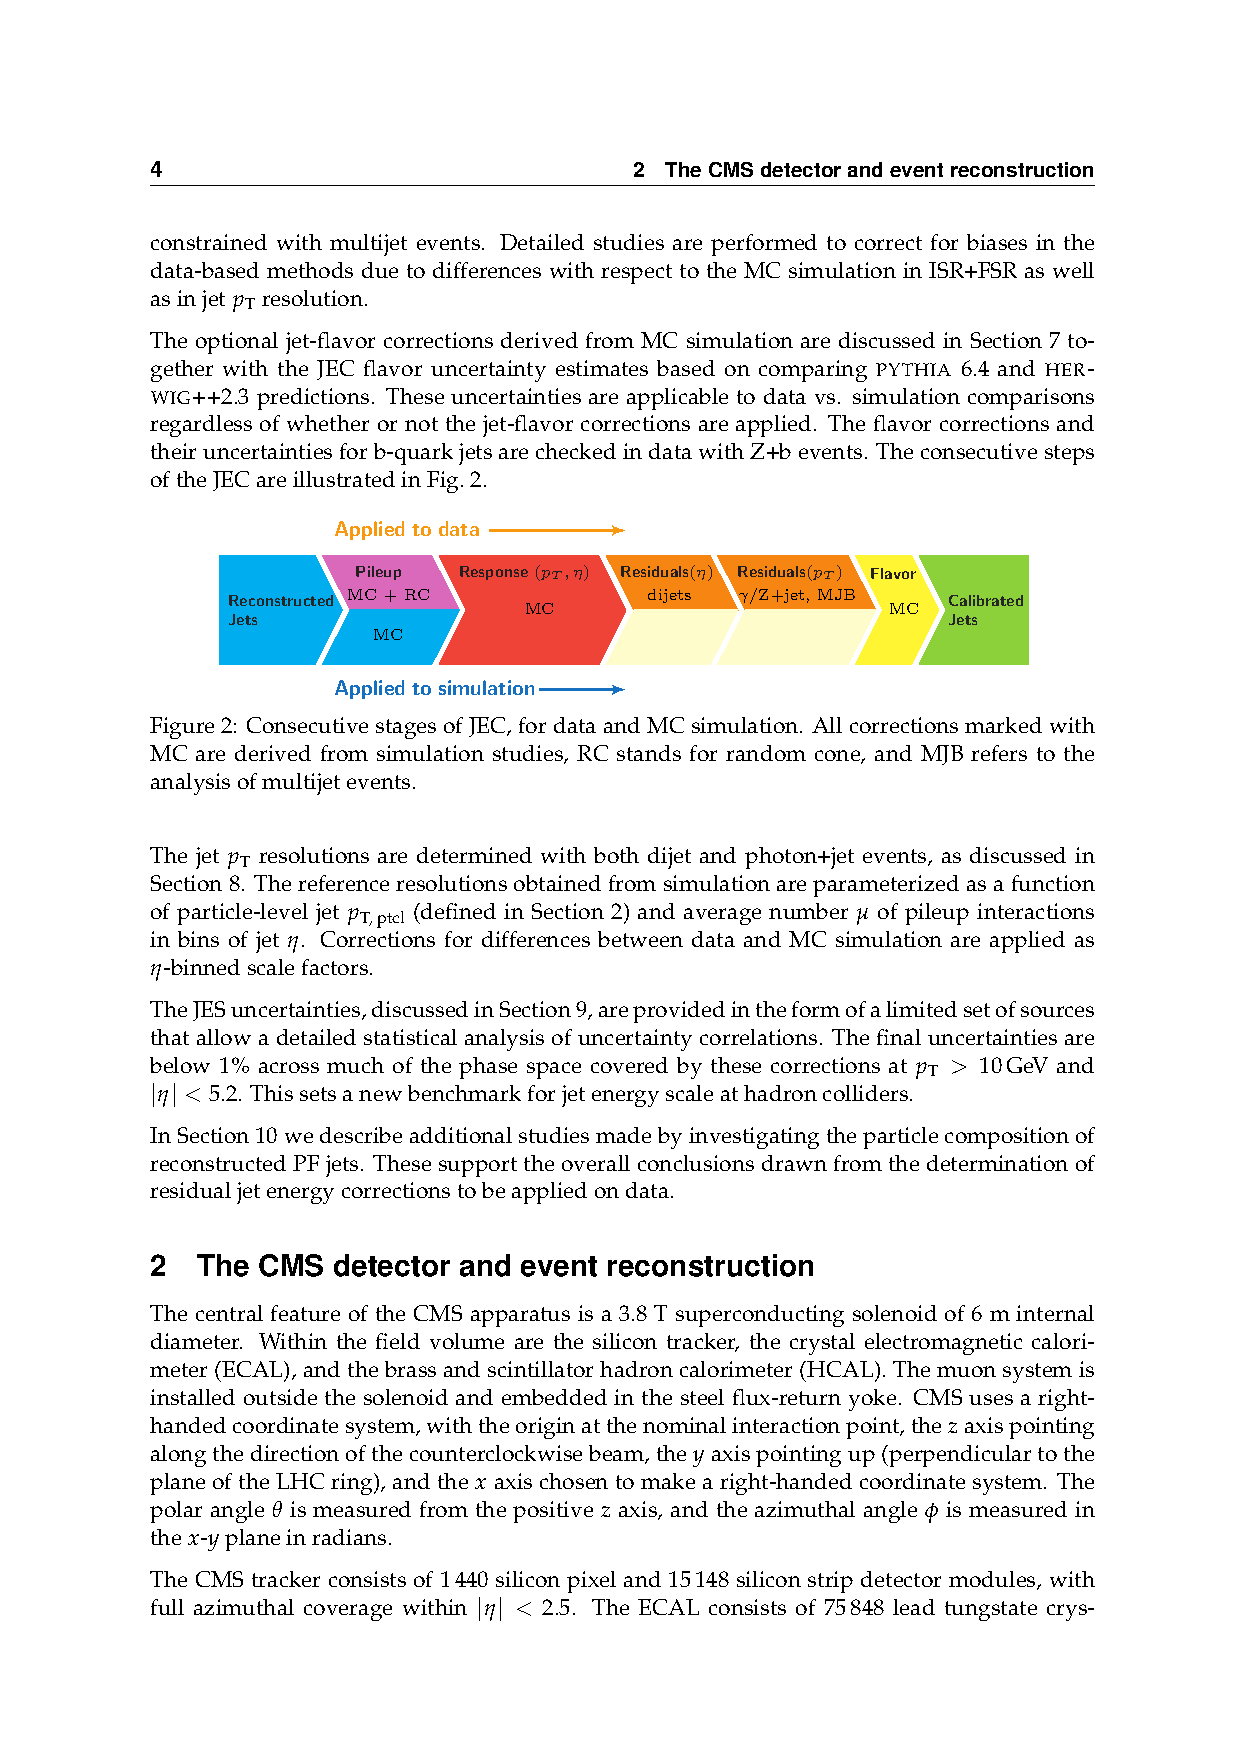
\includegraphics[width=1.3\textwidth]{/home/anter/Desktop/Thesis/Figures/New/JEC.pdf}\\
 \vspace*{5mm}
 \caption[A schematic diagram of the factorized jet energy corrections (JEC).]{A schematic diagram of the factorized jet energy corrections (JEC) applied to the data (upper half) and simulation (lower half). The reconstructed jets are corrected for pileup effects, non-uniform \pt and $\eta$ response and residual differences between the data and Monte Carlo simulations along with optional flavor corrections. All corrections marked with MC are derived from simulation studies, RC stands for random cone, and MJB refers to the analysis of multijet events. Taken from \cite{Khachatryan:2016kdb}.}
 \label{fig:jec}
 \end{center}
\end{figure}

The corrected jet transverse momentum $p^{\rm corr}_{\rm T}$ is obtained by applying all correction factors subsequently on raw or uncorrected jet transverse momentum $p^{\rm raw}_{\rm T}$ as below :

\begin{equation}
p^{\rm corr}_{\rm T} = c_{\rm res}(\eta,p''_{\rm T})\cdot c_{\rm mc}(\eta,p'_{\rm T})\cdot c_{\rm pileup}(\eta,\rho,{\rm A}_{j},p^{\rm raw}_{\rm T})\cdot p^{\rm raw}_{\rm T}
\end{equation}
where $p'_{\rm T}$ is the transverse momentum obtained after applying the pileup correction factor $c_{\rm pileup}$ on $p^{\rm raw}_{\rm T}$, $p''_{\rm T}$ is the transverse momentum obtained after applying the additional correction factor $c_{\rm mc}$ because of relative and absolute effects derived from MC. Finally, a correction factor $c_{\rm res}$ is applied for residual effects derived from the data. The corrections applied at each step are discussed below : \\
{\bf Pileup Corrections -} The additional proton-proton collisions occur within the same bunch-crossing along with the main hard interaction and give rise to pileup events. The particles produced from the pileup events get clustered into the jets coming from the hard interaction and increase the jet energy. This extra energy needs to be subtracted from the reconstructed jet energy. This is done by applying the pileup corrections to raw jet $p^{\rm raw}_{\rm T}$. The pileup corrections are determined by simulating a sample of QCD dijet events with and without pileup effects. The pileup correction factor, $c_{\rm pileup}$ is calculated from jet area method using the pileup density $\rho$ in the event and the jet area ${\rm A}_{j}$. $c_{\rm pileup}$ is parametrized as a function of $\rho$, ${\rm A}_{j}$, jet \pt and $\eta$. There are corrections for residual differences between the data and detector simulation which are determined using the random cone (RC) method in zero-bias events. Hence the different pileup corrections are applied to the data and the MC simulations. \\ \newline
{\bf MC Corrections -} The next correction applied to the pileup corrected jets is based on MC simulated QCD events. Due to the inefficiencies introduced by the detector simulation, the reconstructed jet \pt is not the same as that of the generated one. This difference is corrected with the factor, $c_{\rm mc}$ which is derived by comparing the measured jet \pt to the particle level jet \pt. The corrections are determined as a function of jet \pt and $\eta$ which make the detector response uniform over these two variables. \\ \newline
{\bf Residual Data Corrections -} The jets corrected with above mentioned corrections are further corrected for remaining small differences between the data and MC simulations. This correction is applied only to the data. The correction factor $c_{\rm res}$ is derived using data-driven methods. The relative residual corrections are evaluated using dijet events in which a probe jet is calibrated using a tag jet. The last correction applied is the absolute residual correction in which the precisely reconstructed $Z$ bosons balanced to a jet are used to calibrate the jet energy. \\ \newline
{\bf Flavor Corrections -} These corrections correct the jets for flavor dependence (b, $\tau$ etc.) and are optional. These are extracted using Z\plusn jet and photon\plusn jets simulated events. %The flavor corrections have not been applied for 8 TeV CMS data.
\\}
\end{itemize}
\end{frame}
%\end{comment}
%##################################### Slide : 3 ###########################################
\begin{frame}
\frametitle{\centerline{Multijet Cross-Sections and their Ratio \ratio}}
\setlength\labelsep   {\dimexpr\labelsep + 0.05em\relax}
\setlength\leftmargini{\dimexpr\leftmargini + 0.05em\relax}
\begin{itemize}
\item {\scriptsize The scale based on the transverse momentum of the jets is used :
\begin{align*}
\blue{\resizebox{.32\hsize}{!}{$\ptave = \mathrm{\frac{p_{T,1}~\plus p_{T,2}}{2} = \httwo}}}
\end{align*}
\item Inclusive differential multijet event cross section is defined as : \\}
\vspace{-6mm}
\begin{align*}
\resizebox{.45\hsize}{!}{$\mycolor{\mathrm{\frac{d\sigma}{d(\httwons)}} =  \frac{1}{\epsilon~\mathcal{L}_{\mathrm{int,eff}}}\frac{N_\mathrm{event}}{\Delta\big(\httwons\big)}}$} %~~~~\mathrm{where}$}
\end{align*}
\begin{comment}
\cir
\begin{itemize}
\begin{itemize}
\vspace{-4mm}
{\scriptsize \item $\epsilon$ : the product of the trigger and jet selection efficiencies and $>$ 99\%,
\item $\mathcal{L}_{\mathrm{int,eff}}$ : the effective integrated luminosity,
\item $\it{N}_\mathrm{event}$ : the number of 2- or 3-jet events counted in an \httwo bin, and
\item $\Delta\big(\httwons\big)$ : the bin widths. The measurements are reported in units of (pb/GeV). \\}
\end{itemize}
\end{itemize}
\vspace{0.5mm}
\ball
%\end{comment}
\item {\scriptsize Inclusive $n$\hy jet event samples include the events with number of jets $\geq$ $n$.\\}
\begin{itemize}
\tri
\item {\scriptsize $n$ = 2 $\rightarrow$ Inclusive 2-jet events \blue{(\njt)}
\item $n$ = 3 $\rightarrow$ Inclusive 3-jet events \blue{(\njth)}\\}
\end{itemize}
\item {\scriptsize %The cross-section ratio \rations, defined in Eq.~\ref{eq:ratio_32} is obtained by dividing the differential cross-sections of inclusive 3\hy jet events to that of inclusive 2\hy jet one, for each bin in \httwo. \ratio = \frac{{\dd{\sigma_{3\hy {\rm jet}}}{\big(\httwo\big)}}}{\dd{\sigma_{2\hy {\rm jet}}}{\big(\httwo\big)}}
\begin{equation}
 \label{eq:ratio_32}
 \ratio = \frac[10pt]{{\dd{\sigma_{3\hy {\rm jet}}}{\big(\httwo\big)}}}{\dd{\sigma_{2\hy {\rm jet}}}{\big(\httwo\big)}}
\end{equation}
For inclusive 2-jet events sufficient data are available up to \httwo \ls 2000 GeV, while for inclusive 3-jet events and the ratio \rations, the accessible range is limited to \httwo \ls 1680 GeV. In the talk : \\}
\tri
\begin{itemize}
\item {\scriptsize Highlighted text in \green{green} $\rightarrow$ {\bf changed during ARC review}
\vspace{1.0mm}
\item Inclusive 2\mbox{-}jet : {\bf $\rm{n_{ j} \geq}$~2} \green{(300--2000 GeV)}, Inclusive 3\mbox{-}jet : {\bf $\rm{n_{ j} \geq}$~3} \green{(300--1680 GeV)}, Inclusive 4\mbox{-}jet : {\bf $\rm{n_{ j} \geq}$~4} \mycolor{(only in AN for now)} and ratio : \ratio \green{(300--1680 GeV)} \\}
\end{itemize}
\end{itemize}
\end{frame}
\ball

%##################################### Slide : 16 ###########################################
\begin{frame}
\frametitle{\centerline{Next-to-leading order (NLO) Calculations}}
\setlength\labelsep   {\dimexpr\labelsep + 0.05em\relax}
\setlength\leftmarginiii{\dimexpr\leftmarginiii + 0.05em\relax}
\vspace{-3.5mm}
\begin{center}
\begin{itemize}
\item {\scriptsize The NLO theoretical calculations are done using the parton-level generator NLOJet\plus\plus within the fastNLO framework.
\vspace{1mm}
\item The renormalization and factorization scales (\mur~and \muf) are equal to \httwo.
\vspace{1mm}
\item Used different PDF sets (details on next slide) 
\vspace{1mm}
\item Uncertainties due to renormalization and factorization are evaluated by varying the default scale \httwo chosen for \mur~ and \muf~ independently in the following six combinations (\mur/\httwo,\muf/\httwo)=(1/2,1/2), (1,1/2), (1/2,1), (1,2), (2,1) and (2,2)
\vspace{1mm} 
\item k-factor is calculated as : \\}
\end{itemize}
\vspace{-10.5mm}
\begin{align*}
\hspace{8mm}\resizebox{.35\hsize}{!}{$\rm k_{fac} = \frac{\sigma_{NLO}}{\sigma_{LO}},~ k_{fac}{^\ratio} = \frac{k_{fac}^{3-jet}}{k_{fac}^{2-jet}}$}
\end{align*}
\vspace{-2.mm}
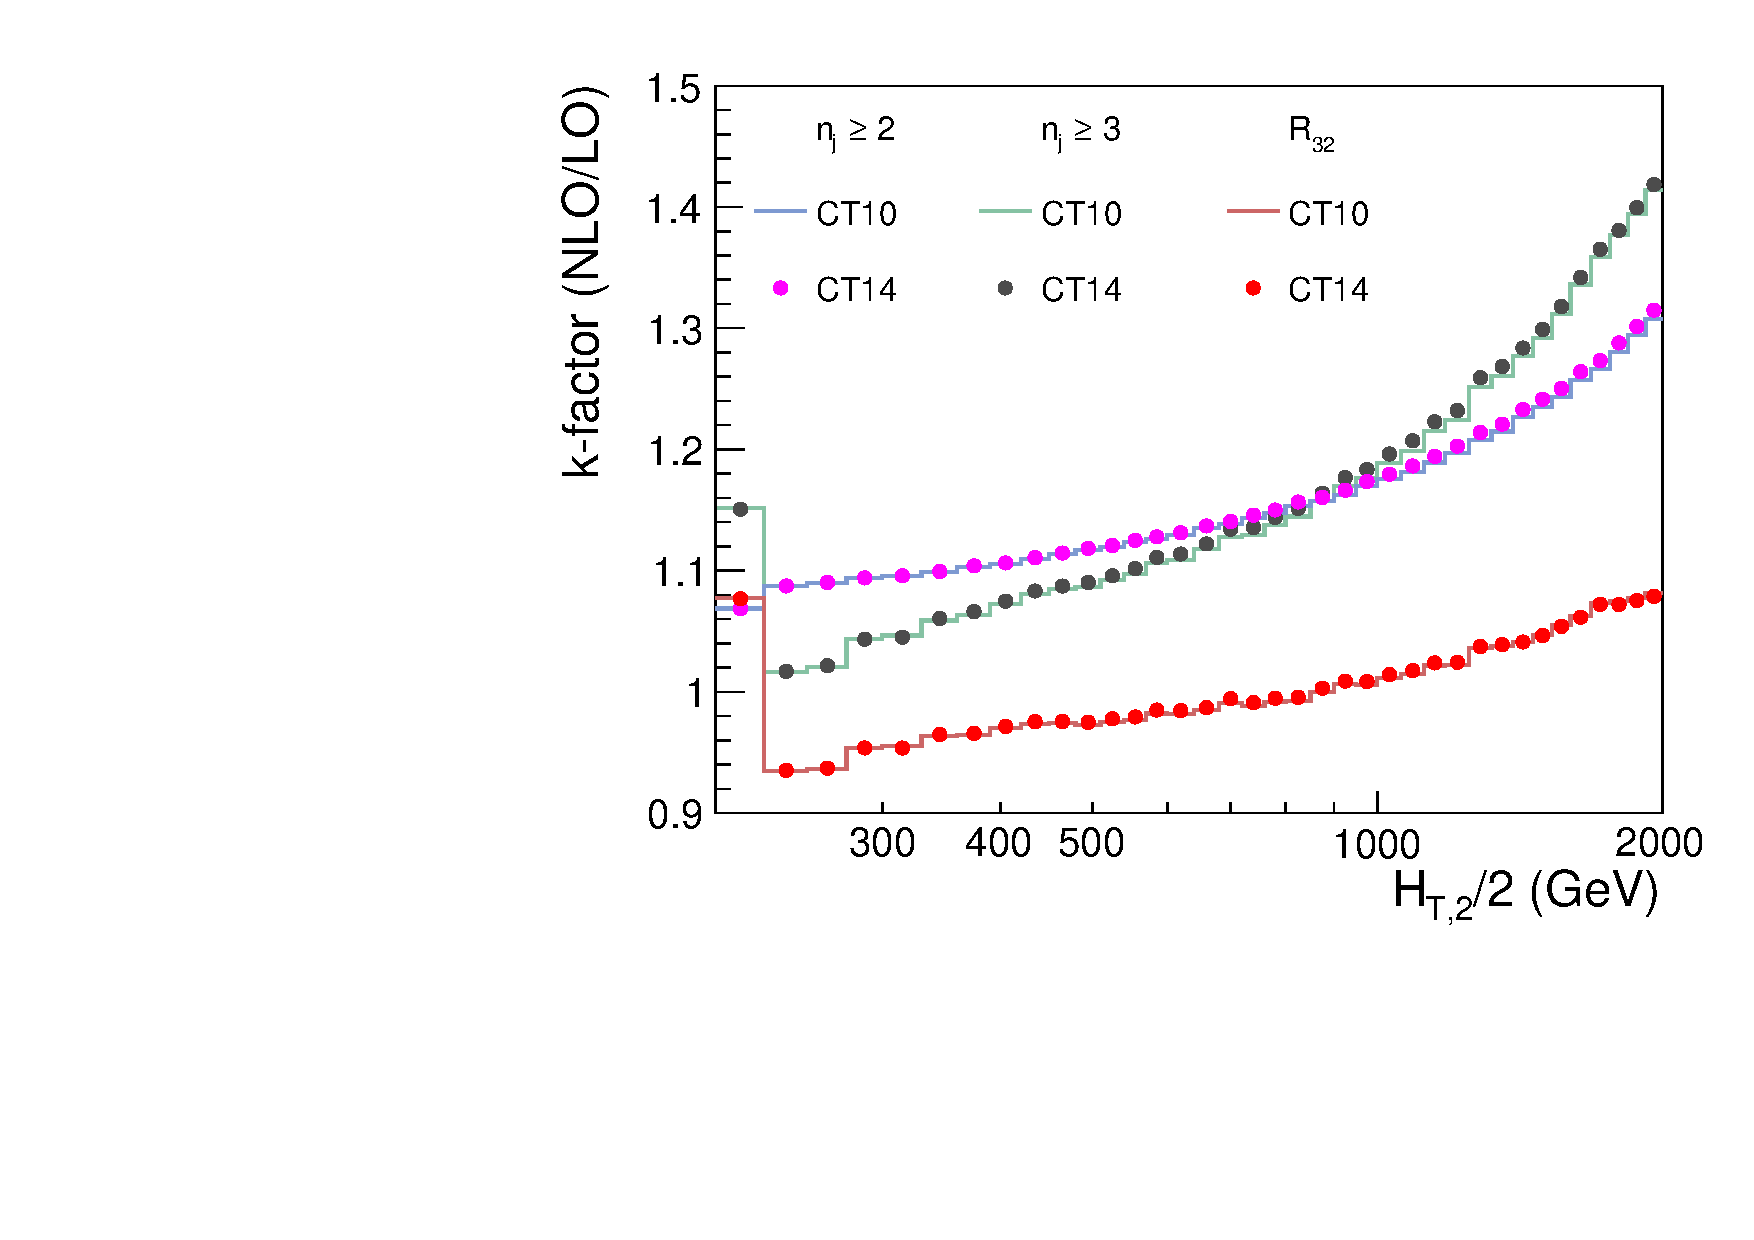
\includegraphics[scale = 0.23]{/home/anter/Desktop/Analysis_8/Present_Latex/Approval/Approval/Kfactor_all_1.pdf}\\
%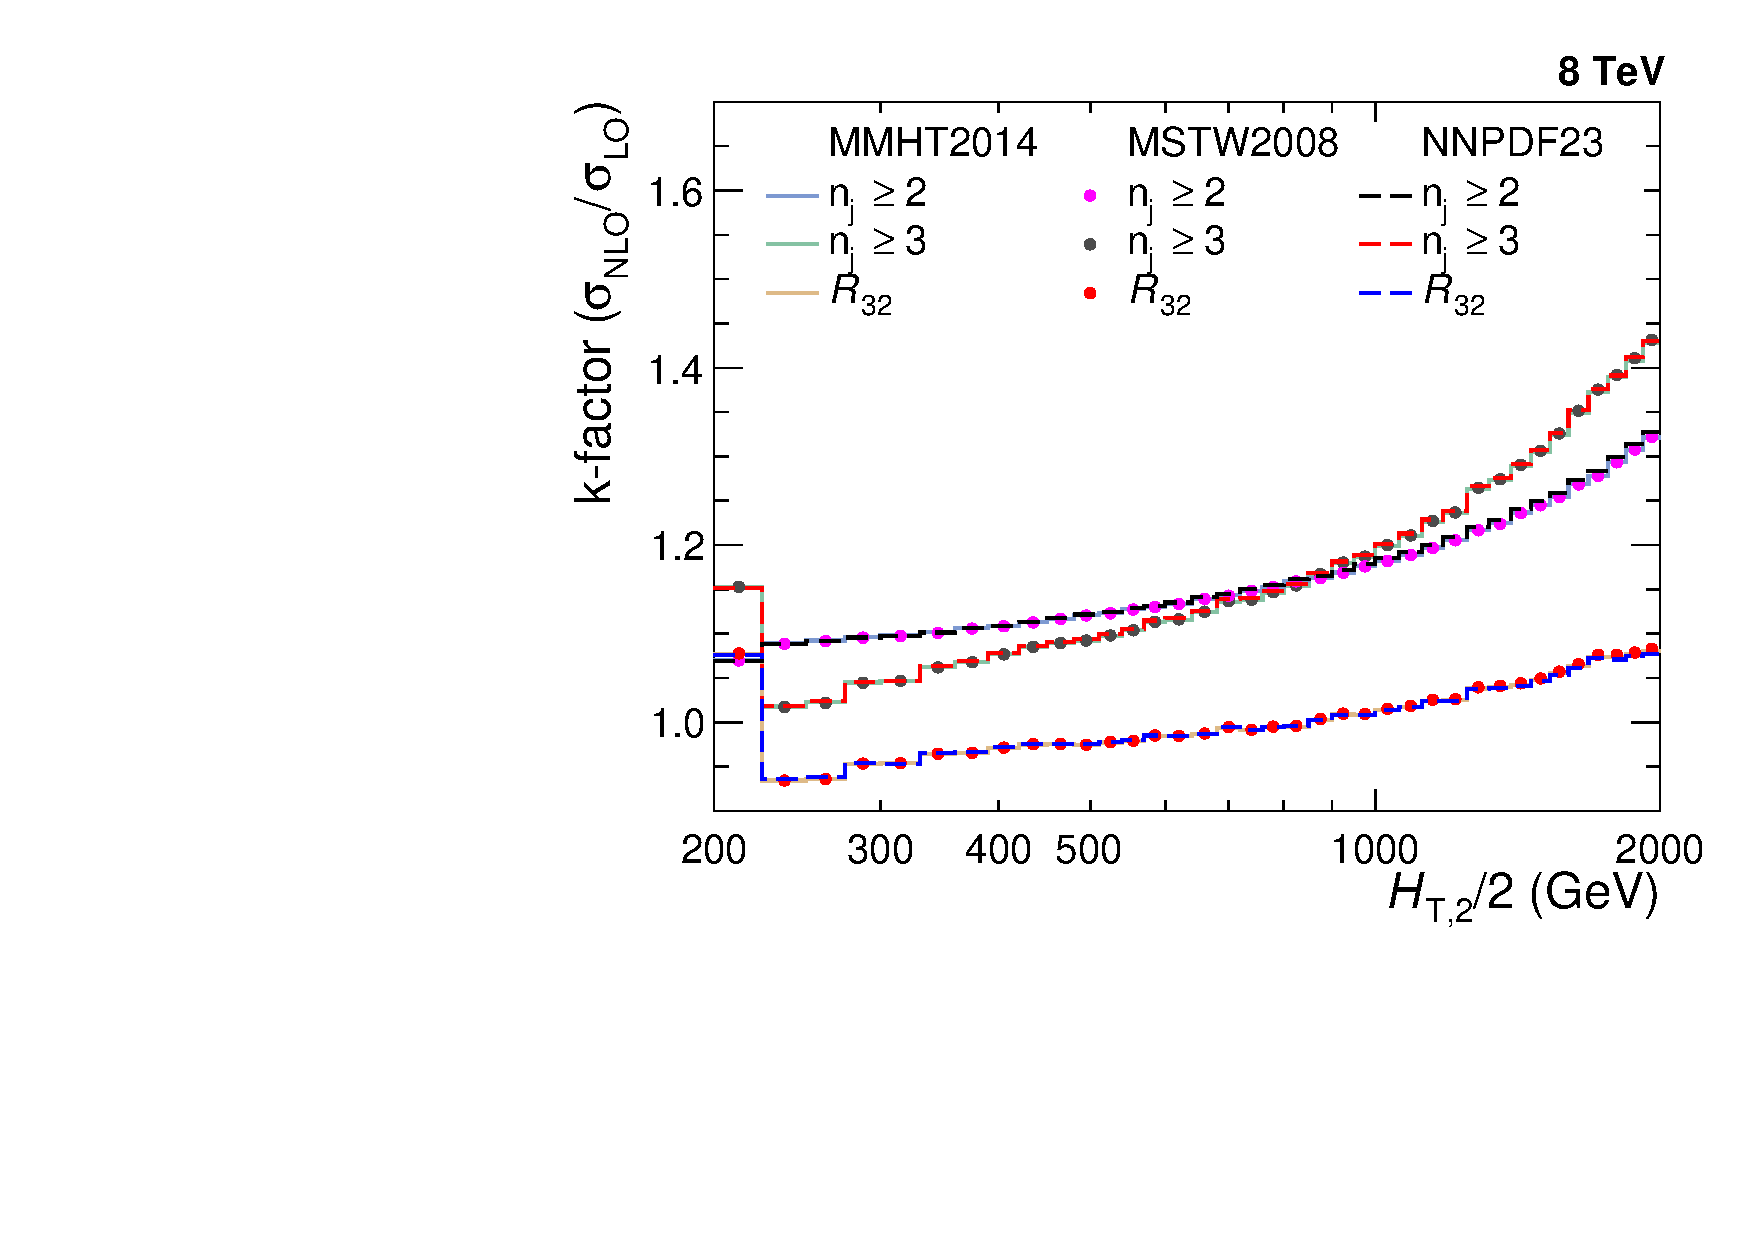
\includegraphics[scale = 0.19]{/home/anter/Desktop/Analysis_8/Present_Latex/After_Pre-approval/New_Plots_PAS/Kfactor_all_2.pdf}\\

\begin{itemize}
\item {\scriptsize kfactor jumps at lowest \httwo for inclusive 3-jet events : Below 225 GeV some jet configurations are kinematically forbidden and the first few bins shown still suffer from these kinematical effects
\vspace{0.2mm}
\item Final analysis cut requires \httwo $>$ 300 GeV\\}
\end{itemize}
\end{center}
\end{frame}

%##################################### Slide : 17 ###########################################
\begin{frame}
\frametitle{\centerline{Details on PDF sets}}
\setlength\labelsep   {\dimexpr\labelsep + 0.05em\relax}
\setlength\leftmarginiii{\dimexpr\leftmarginiii + 0.05em\relax}
\vspace{-4mm}
\begin{center}
\begin{itemize}
\item {\scriptsize Investigated PDF sets available via LHAPDF6 \\}
\end{itemize}
\vspace{-1.5mm}
\hspace{74mm} \pas
\vspace{-4.mm}
\begin{table}[htbp]
  \centering\tiny
  \begin{tabular}{llccllc}
    \hline\hline
    Base set  & N$_{F}$ & $M_t$ (GeV) &
    $M_Z$ (GeV) &\alpsmz & \alpsmz range\\  \hline
    % LHC Run 1
    ABM11     &    ~ 5   & 180       & 91.174  & $0.1180$   & 0.110--0.130\\
    CT10      & ${\leq}5$ & 172       & 91.188  & $0.1180^*$ & 0.112--0.127\\
    MSTW2008  & ${\leq}5$ & ~$10^{10}$ & 91.1876 & $0.1202$   & 0.110--0.130\\
    NNPDF2.3  & ${\leq}6$ & 175       & 91.1876 & $0.1180^*$ & 0.114--0.124\\\hline
    % LHC Run 2
    CT14      & ${\leq}5$ & 172       & 91.1876 & $0.1180^*$ & 0.113--0.123\\
    HERAPDF2.0& ${\leq}5$ & 173       & 91.1876 & $0.1180^*$ & 0.110--0.130\\
    MMHT2014  & ${\leq}5$ & ~$10^{10}$ & 91.1876 & $0.1180^*$ & 0.108--0.128\\
    NNPDF3.0  & ${\leq}5$ & 173       & 91.2    & $0.1180^*$ & 0.115--0.121\\
    \hline\hline
  \end{tabular}
\end{table}
\vspace{-2mm}
{\tiny A * behind the \alpsmz values signifies that the parameter was fixed, not fitted \\}
%\begin{table}[p]
%  \centering \tiny
%  \begin{tabular}{lcccccc}
%    \hline\hline
%    \multirow{2}{*}{PDF set} & describes & pre-LHC/ & $\sigma$: \chisq &
%    \ratio: \chisq & PDF unc. & \multirow{2}{*}{\alpsmz}\\
%    & jet data & no jets & fit method &
%    fit method & @ each \alpsmz \\\hline
%    CT10       & \checkmark & \checkmark  & OK & OK &    ---     & 0.1180* \\
%    CT14       & \checkmark & ATLAS/CMS   & OK & OK &    ---     & 0.1180* \\
%    MSTW2008   & \checkmark & \checkmark  & OK & OK &    ---     & 0.1202  \\
%    MMHT2014   & \checkmark & ATLAS/CMS   & OK & OK &    ---     & 0.1180* \\
%    NNPDF2.3   & \checkmark & ATLAS       &  ? & OK & \checkmark & 0.1180* \\
%    ABM11      &     ---    & \checkmark  & OK & OK &    ---     & 0.1180  \\
%    \hline\hline
%  \end{tabular}
%\end{table}
\vspace{0.5mm}
\begin{itemize}
\item {\scriptsize Out of these eight PDF sets the following three will not be considered further :
\tri
\begin{itemize}
\item {\scriptsize ABM11 : do not describe LHC jet data at small jet rapidity
\vspace{1mm}
\item HERAPDF2.0 : exclusively fits HERA DIS data with only weak constraints on the gluon PDF
\vspace{1mm}
\item NNPDF3.0 : the range in values available for \alpsmz is too limited \\}
\end{itemize}
\vspace{1mm}
\ball
\item \green{MSTW2008, MMHT2014 : 10$^{10}$ $\rightarrow$ Five flavours, with top quark mass $\approx$ infinity} \\} 
\end{itemize}
\end{center}
\end{frame}

%##################################### Slide : 18 ###########################################
\begin{frame}
\frametitle{\centerline{Non-Perturbative (NP) Corrections}}
\setlength\labelsep   {\dimexpr\labelsep + 0.05em\relax}
\setlength\leftmarginiii{\dimexpr\leftmarginiii + 0.05em\relax}
\vspace{-2mm}
\begin{itemize}
{\scriptsize \item NP corrections are required to the NLO spectrum, to compare with the experimental measurement. \\
\tri
\begin{itemize}
{ \scriptsize \item LO generators : Pythia6 Z2* and Herwig\plus\plus (tune 2.3) 
\item NLO generator : \green{Powheg\plus Pythia8 CUETS1}\\}
\end{itemize}
\ball
\vspace{-1.mm}
\item NP factor is obtained by switching MPI and hadronization on/off, {$\rm c^{NP} = \frac{\sigma^{PS\plus~HAD\plus~MPI}}{\sigma^{PS}}$}
\vspace{0.3mm}
\item Mean value of the envelope taken gives the NP factor and the envelope covering all differences taken as uncertainty. 
  \vspace{0.2mm}
  \item For \ratio : first the ratio of cross sections of inclusive 3-jet to that of 2-jet events are taken seperately for hadronization and MPI effects switched off and on. Then the ratio defined above is used to calculate the NP correction factor. \\}
  \end{itemize}
  \vspace{-1.5mm}
  \begin{align*}
    \resizebox{.25\hsize}{!}{$\rm c^{NP}_{\ratio} = \frac{\Big(\frac{\sigma_{3\mbox{-}jet}}{\sigma_{2\mbox{-}jet}}\Big)^{PS\texttt{+}HAD\texttt{+}MPI}}{\Big(\frac{\sigma_{3\mbox{-}jet}}{\sigma_{2\mbox{-}jet}}\Big)^{PS}}$}
  \end{align*}
\vspace{-7.mm}
\begin{center}
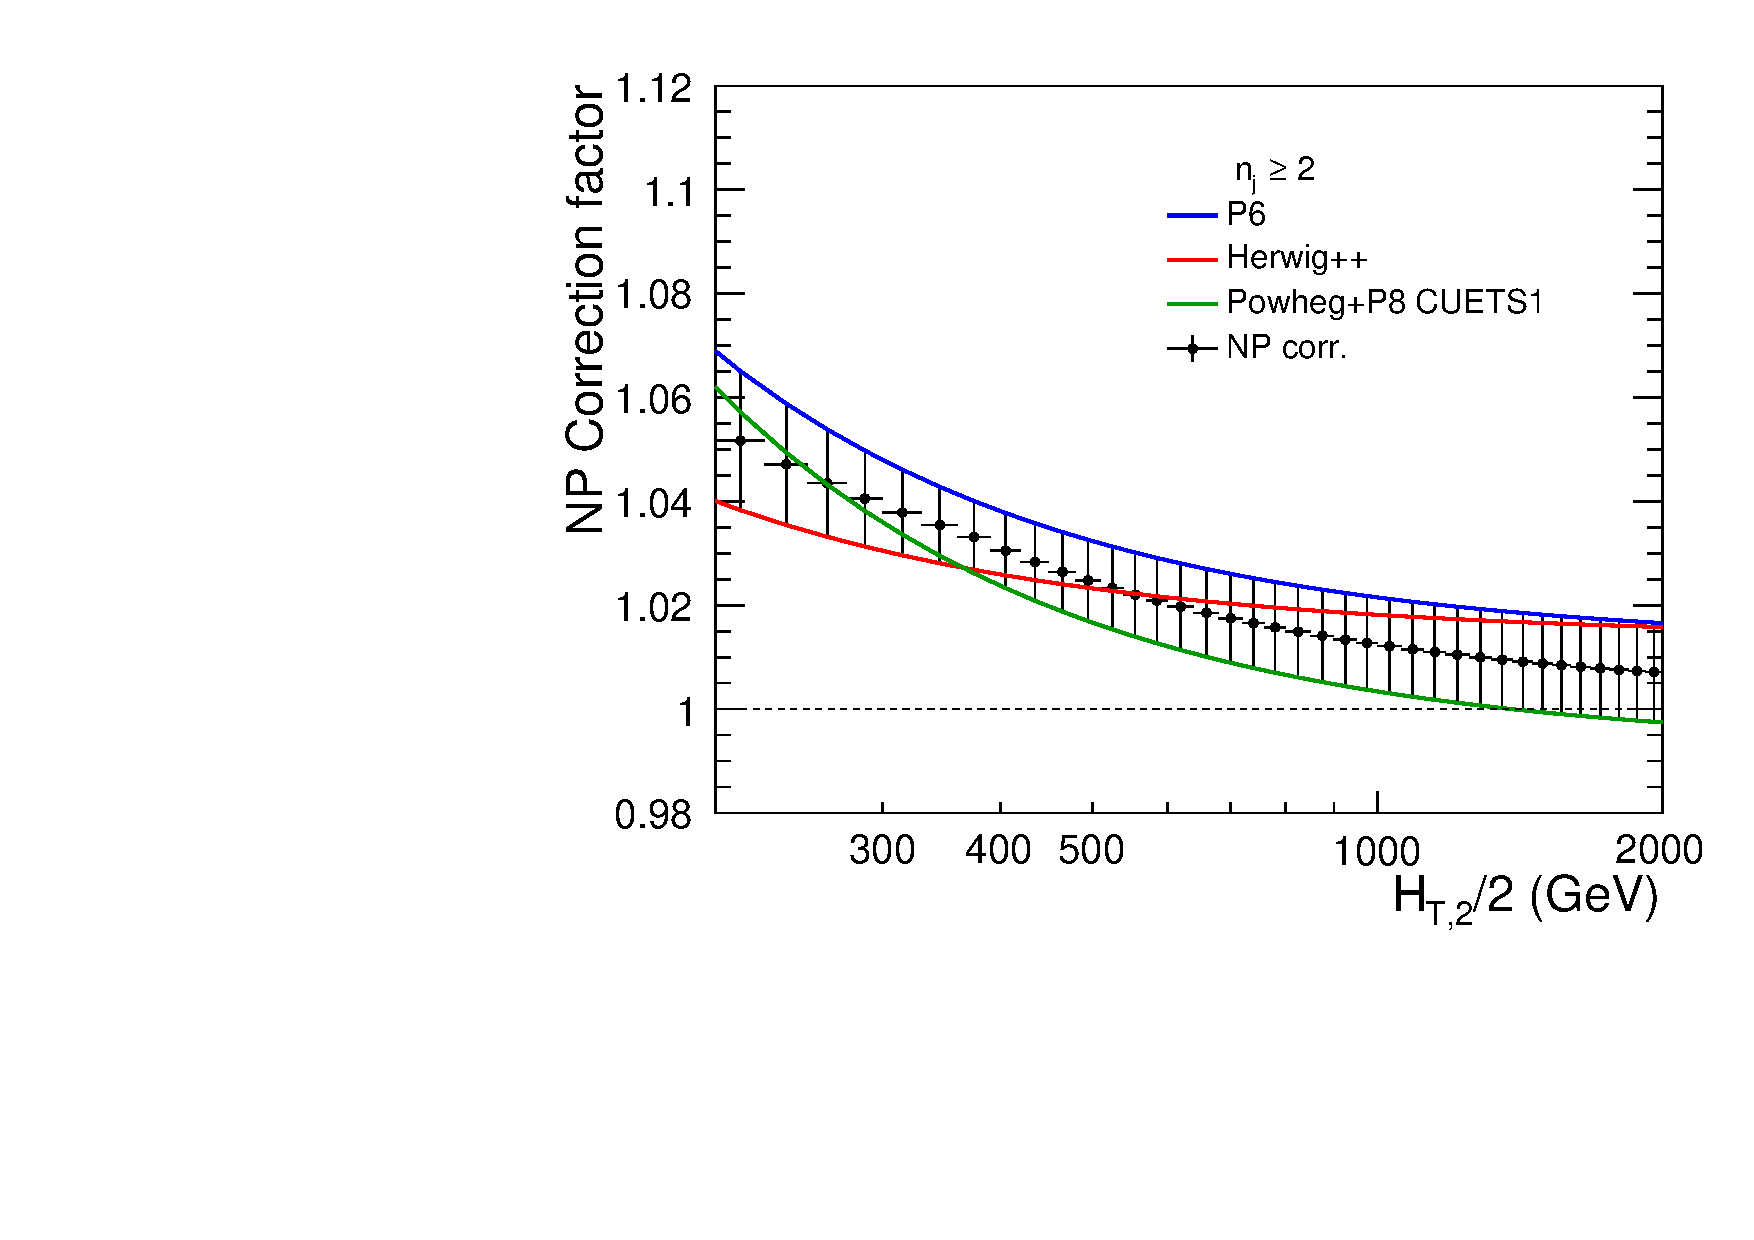
\includegraphics[scale=0.21]{/home/anter/Desktop/Analysis_8/Present_Latex/Approval/Approval_New/Final_NP_Corr_2.pdf}%
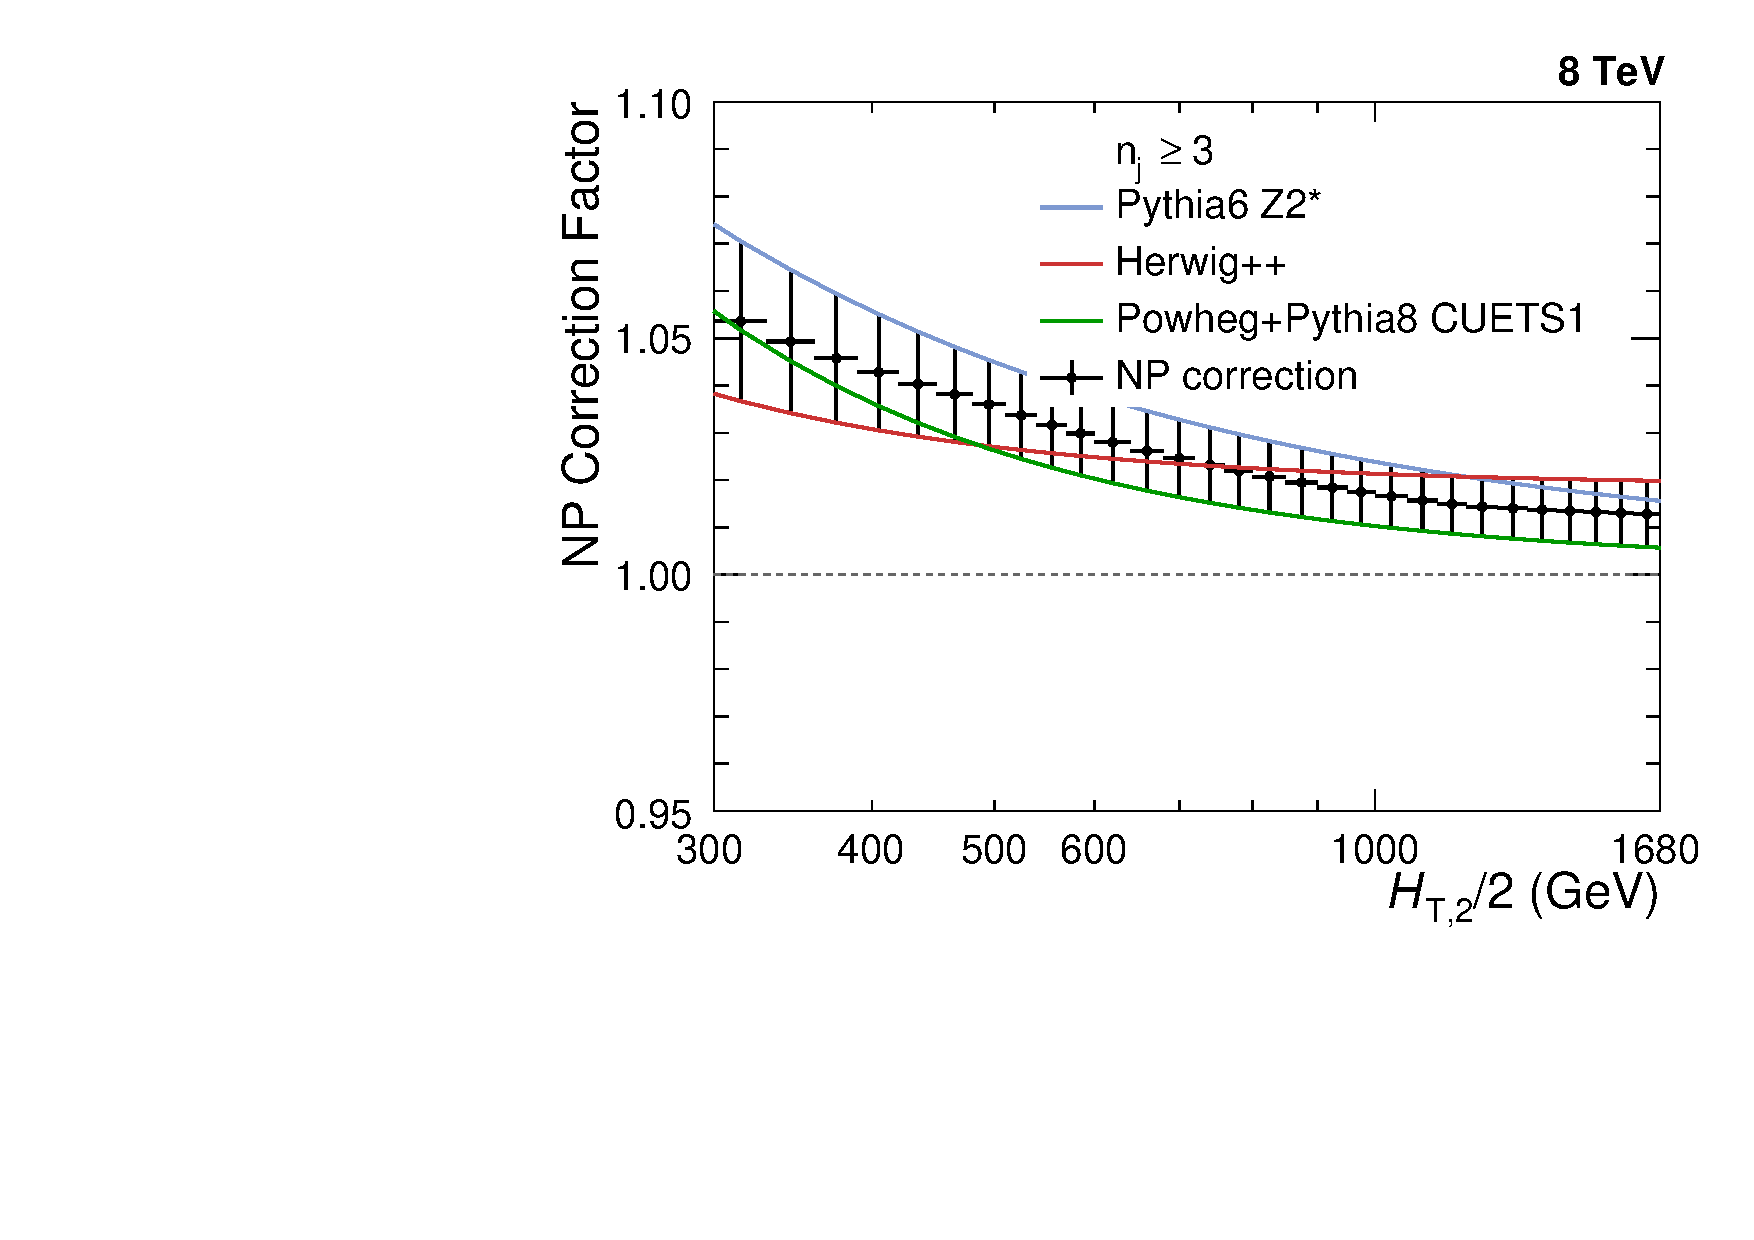
\includegraphics[scale=0.21]{/home/anter/Desktop/Analysis_8/Present_Latex/Approval/Approval_New/Final_NP_Corr_3.pdf}% 
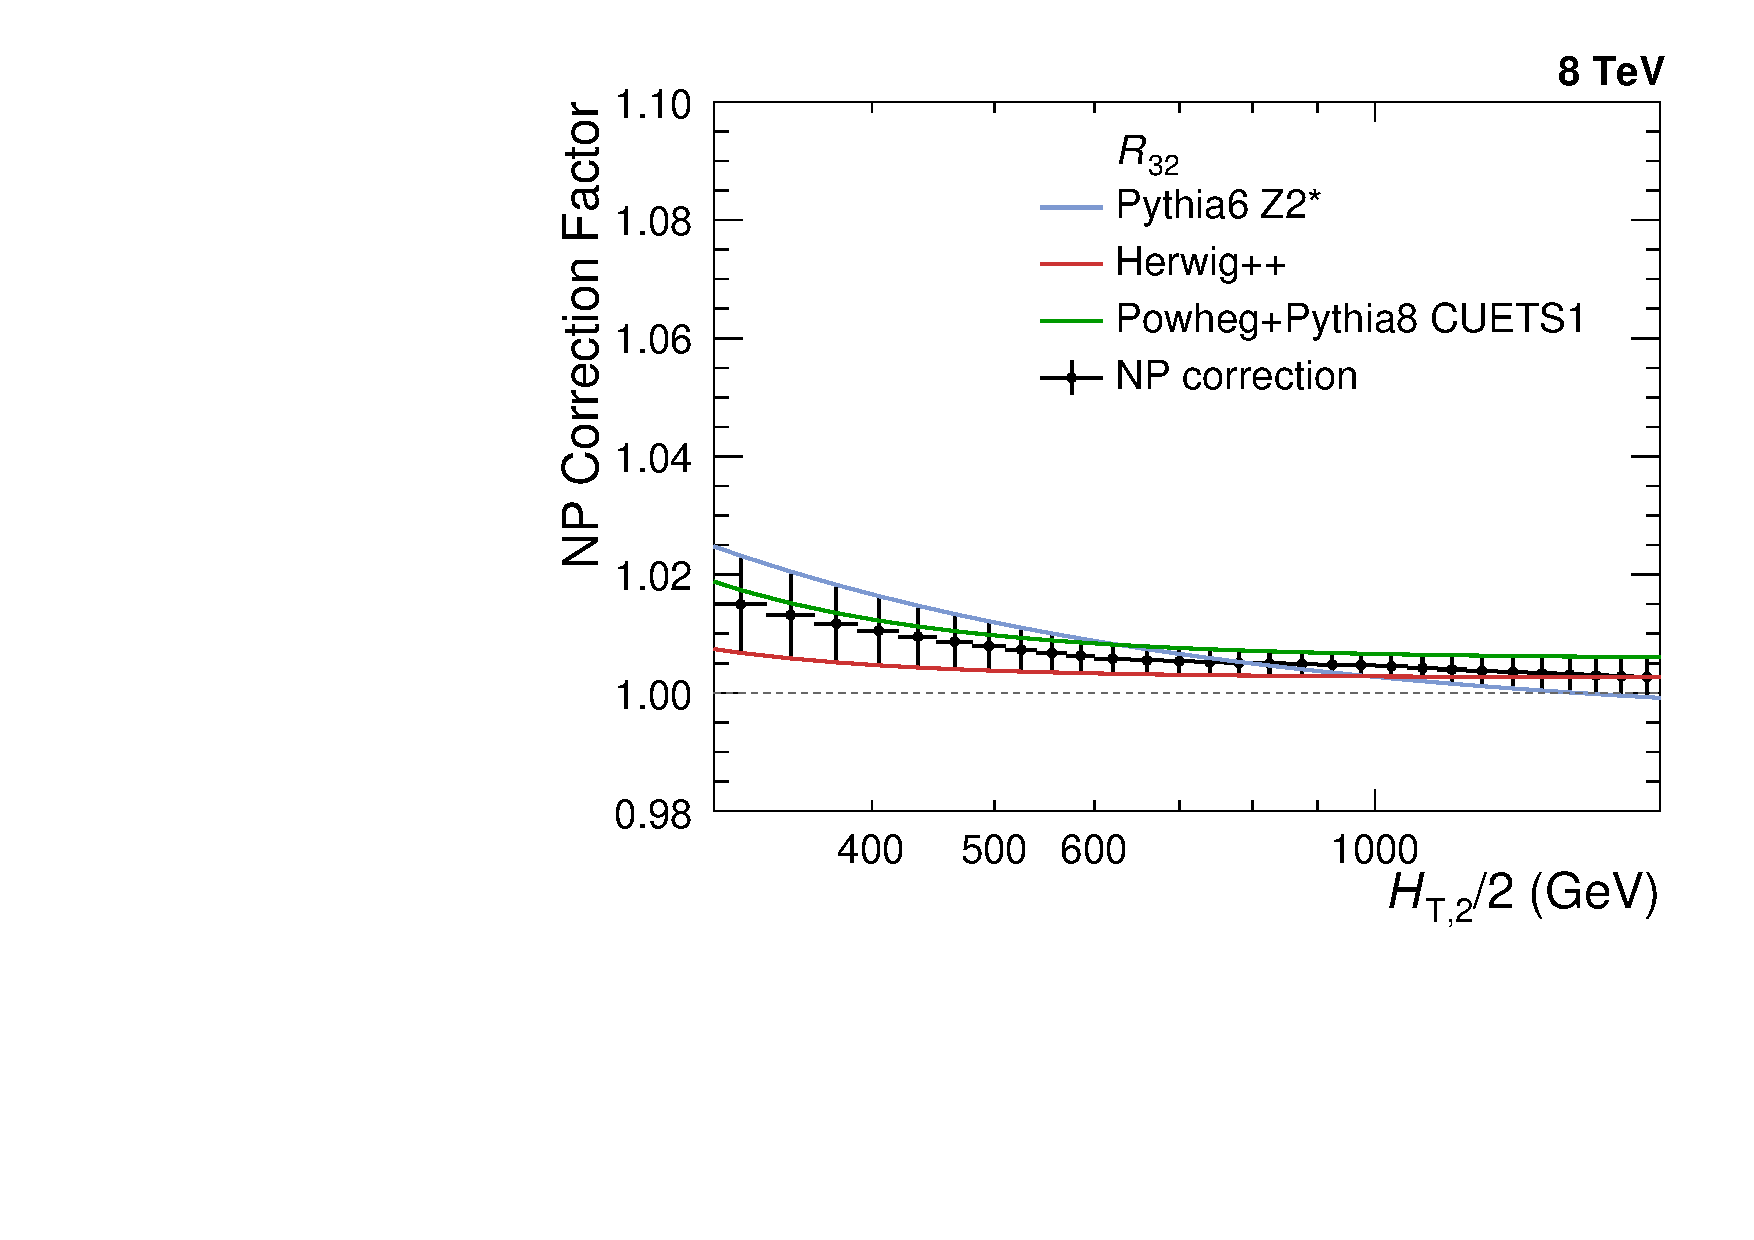
\includegraphics[scale=0.20]{/home/anter/Desktop/Analysis_8/Present_Latex/Approval/Approval_New/Final_NP_Corr_Ratio_32.pdf} \\
\end{center}
\end{frame}

%##################################### Slide : 19 ###########################################
\begin{frame}
\frametitle{\centerline{Electroweak Corrections (EWK)}}
\setlength\labelsep   {\dimexpr\labelsep + 0.05em\relax}
\setlength\leftmarginiii{\dimexpr\leftmarginiii + 0.05em\relax}
\vspace{-2mm}
\begin{itemize}
 \item { \scriptsize EWK account for contributions from electroweak bosons
\vspace{1mm}
\item \green{Only available for inclusive 2-jet} 
\vspace{1mm}
\item Best guess from theory : \\}
\begin{itemize}
\tri
\item {\scriptsize EWK similar for inclusive 2-jet and 3-jet and hence factor of 1 for \ratio \\}
\end{itemize} 
\end{itemize}
\ball
\vspace{-2mm}
\begin{center}
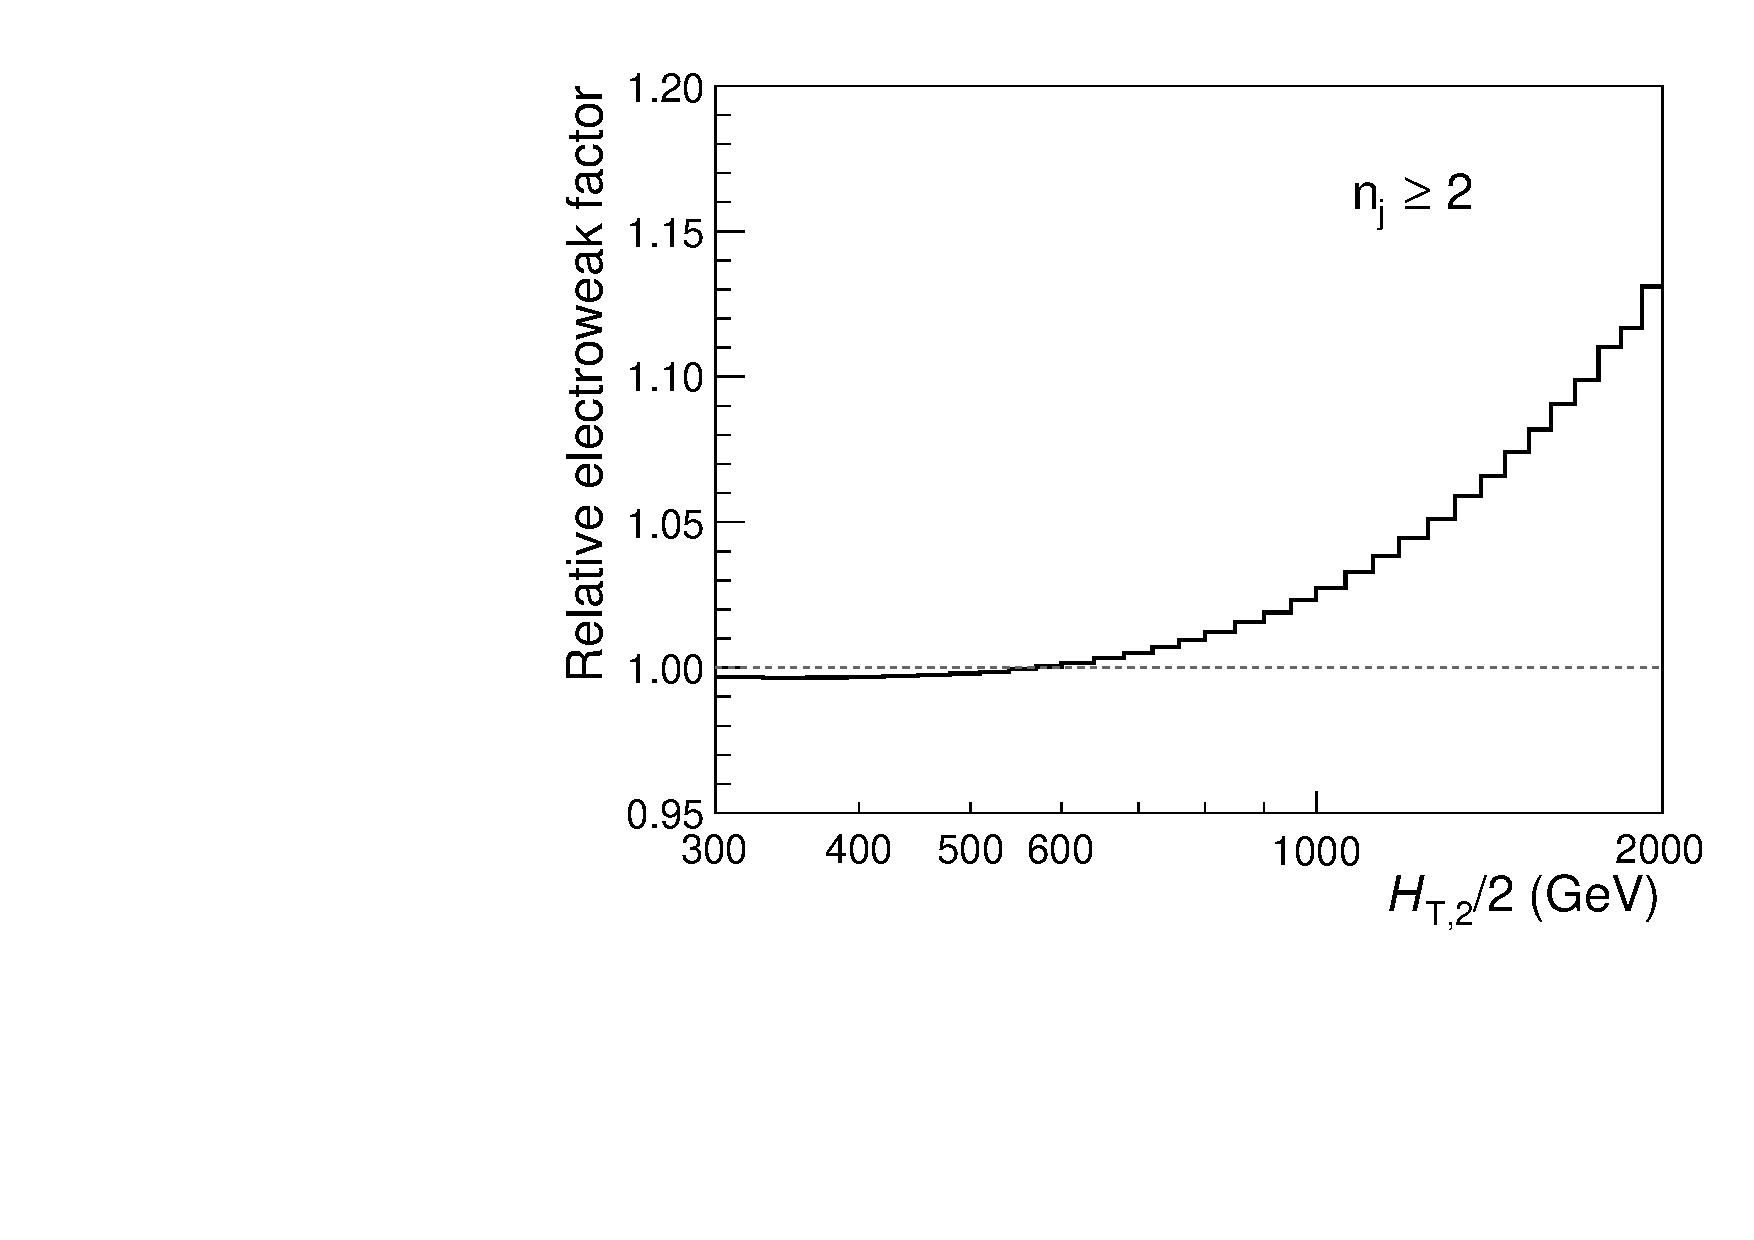
\includegraphics[scale=0.32]{/home/anter/Desktop/Analysis_8/Present_Latex/After_Pre-approval/New_Plots_PAS/EW_2.pdf}
\end{center}
\end{frame}

%##################################### Slide : 20 ###########################################
\begin{frame}
\frametitle{\centerline{Theoretical Uncertainties}}
\setlength\labelsep   {\dimexpr\labelsep + 0.05em\relax}
\setlength\leftmarginiii{\dimexpr\leftmarginiii + 0.05em\relax}
\vspace{-1mm}
\begin{center}
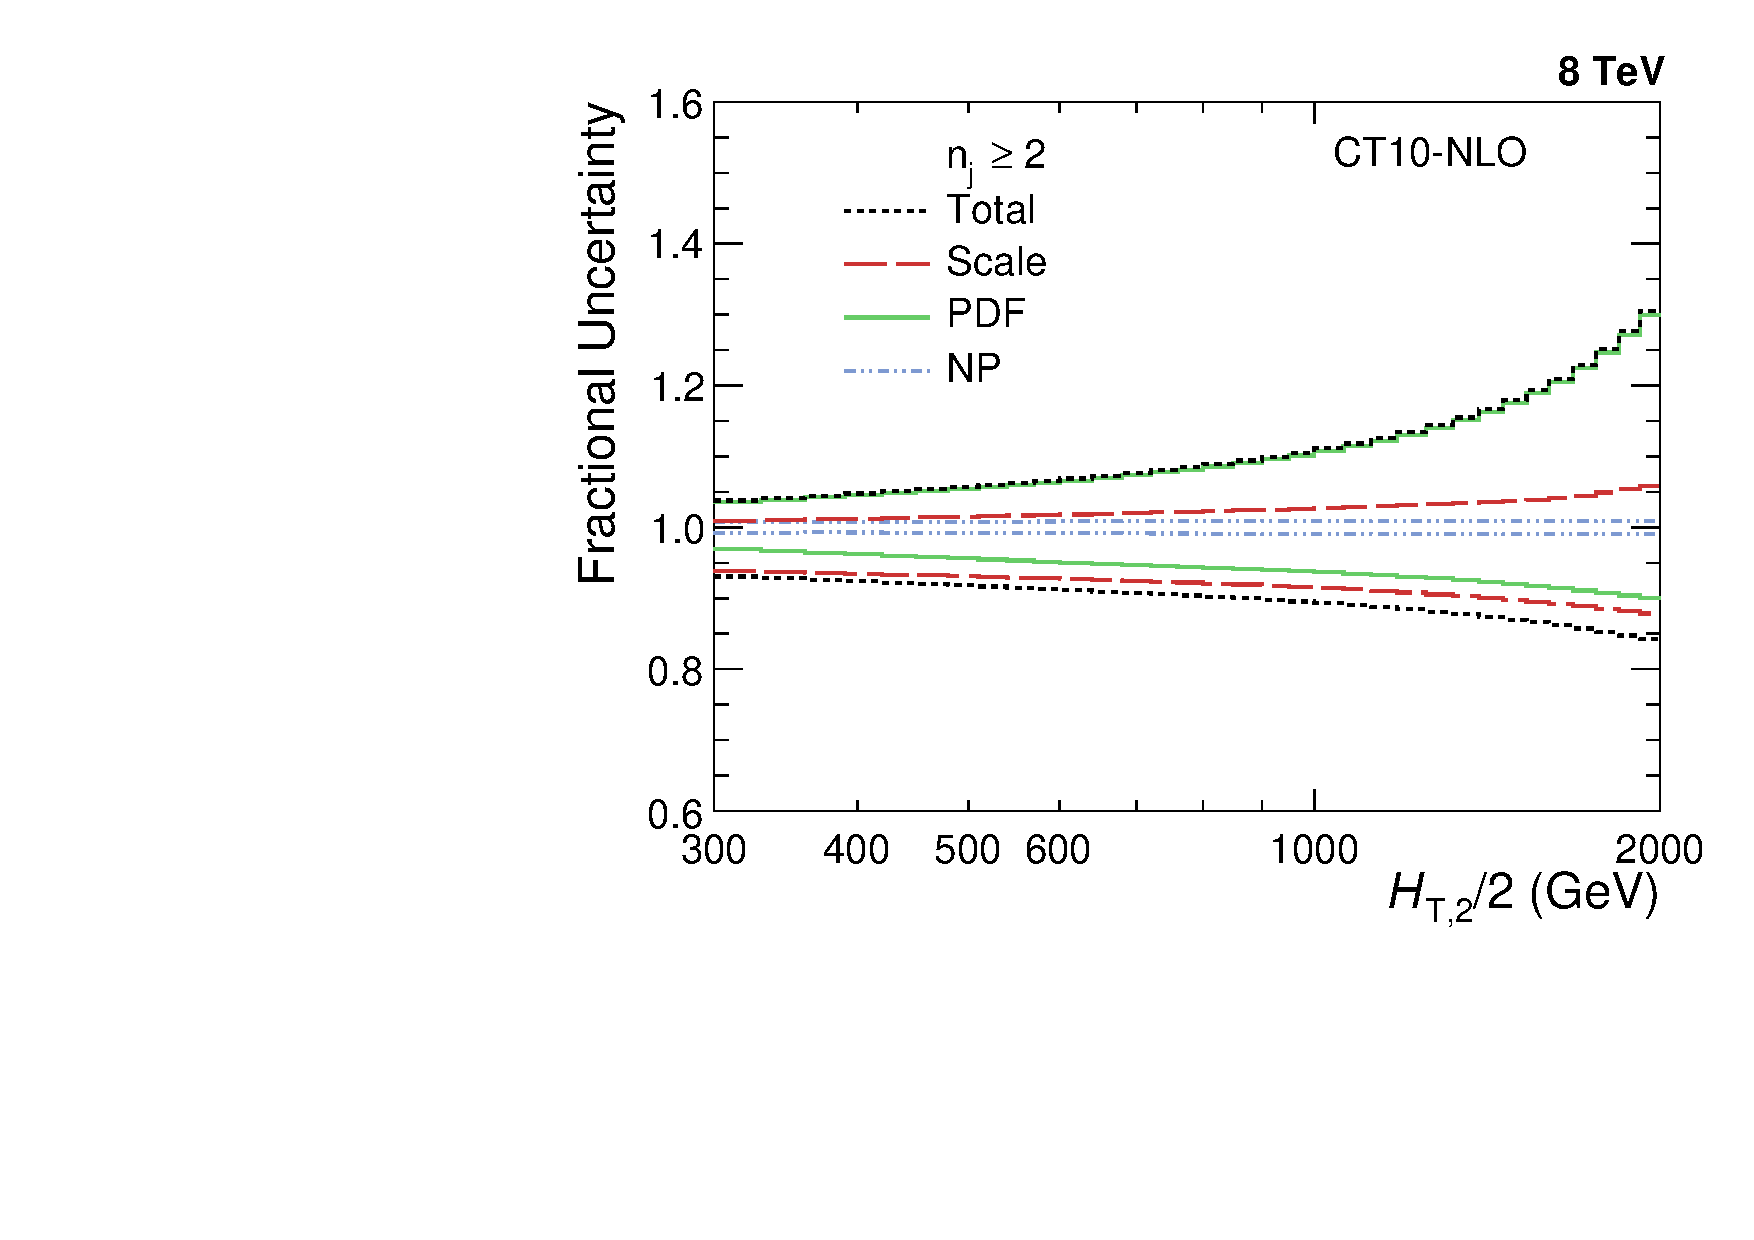
\includegraphics[scale = 0.25]{/home/anter/Desktop/Analysis_8/Present_Latex/Approval/Approval_New/Theory_Unc_2.pdf}%
\hspace{4mm}
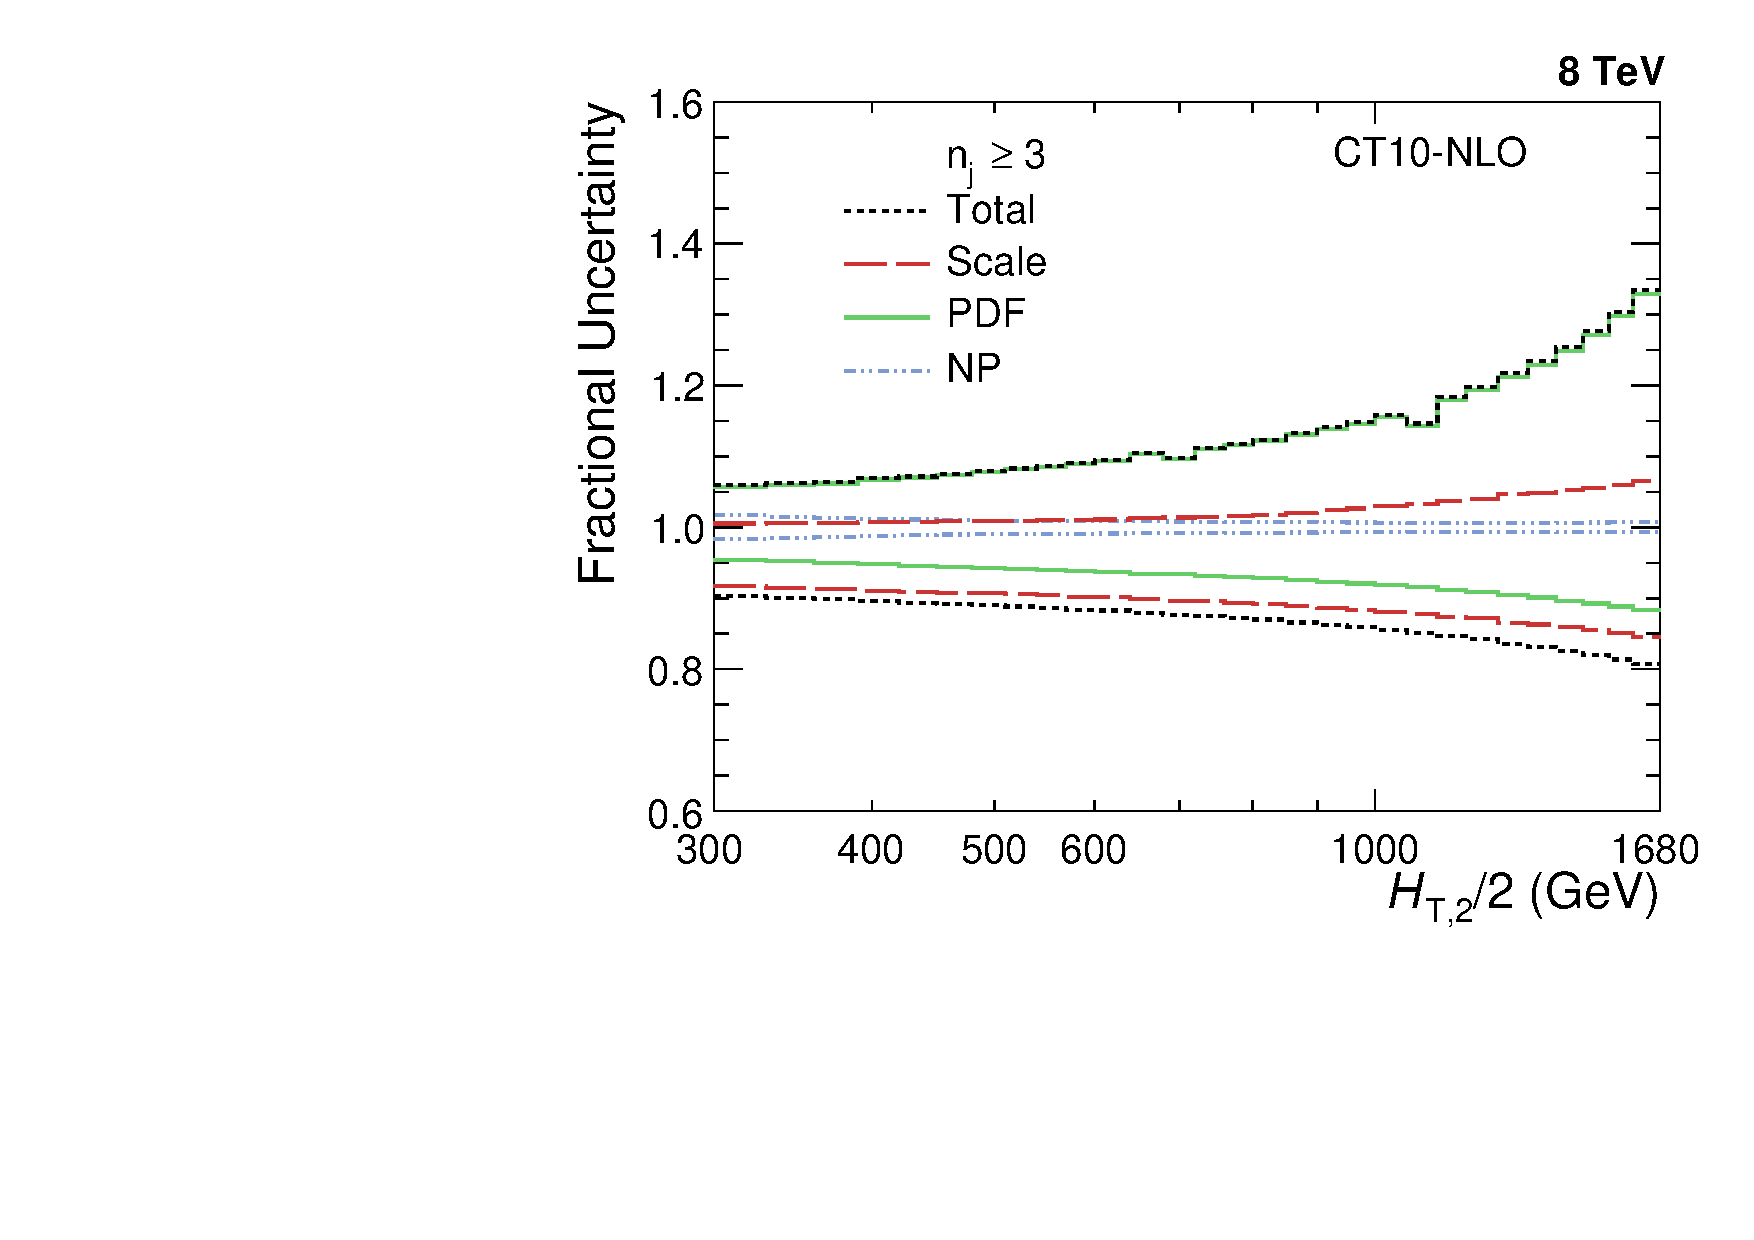
\includegraphics[scale = 0.25]{/home/anter/Desktop/Analysis_8/Present_Latex/Approval/Approval_New/Theory_Unc_3.pdf} \\
\end{center}
\vspace{-3mm}
\begin{minipage}[tbp]{0.4\textwidth}
\vspace{-6mm}
\begin{table}[t]
  \centering\tiny
   %\begin{tabular}{cccc}
   \begin{tabular}{ >{\centering\arraybackslash}m{0.6in} >{\centering\arraybackslash}m{0.53in} >{\centering\arraybackslash}m{0.53in} >{\centering\arraybackslash}m{0.55in} }
    \hline\hline
     Uncertainty Source & {\bf Inclusive 2-jet} & {\bf Inclusive 3-jet} & {\bf \ratio}\\\hline
      {\bf \textcolor{red} {Scale}} & 5 to 13\% & 11 to 17\% & 6 to 8\% \\
     {\bf \textcolor{green!50!white} {PDF}} & 2 to 30\% & 2 to 30\% & 2 to 7\% \\
     {\bf \textcolor{blue} {NP}} & 4 to 5\% & 4 to 5\%  & 1\% \\
     \hline\hline
  \end{tabular}
\end{table}
\vspace{-3mm}
%\begin{itemize}
%\item \tiny {\green {Small dips at 1.X TeV in the PDF uncertainty (top right) : It is a feature of the CT10 PDF. Likewise the smaller dip at 700 GeV. If another PDF, e.g. CT14, is used, these dips are gone (Slide No.~\ref{theory_unc} in Back-Up). } \\}
%\end{itemize}
\end{minipage}
\hspace{24mm}
\begin{minipage}[tbp]{0.25\textwidth}
\vspace{1mm}
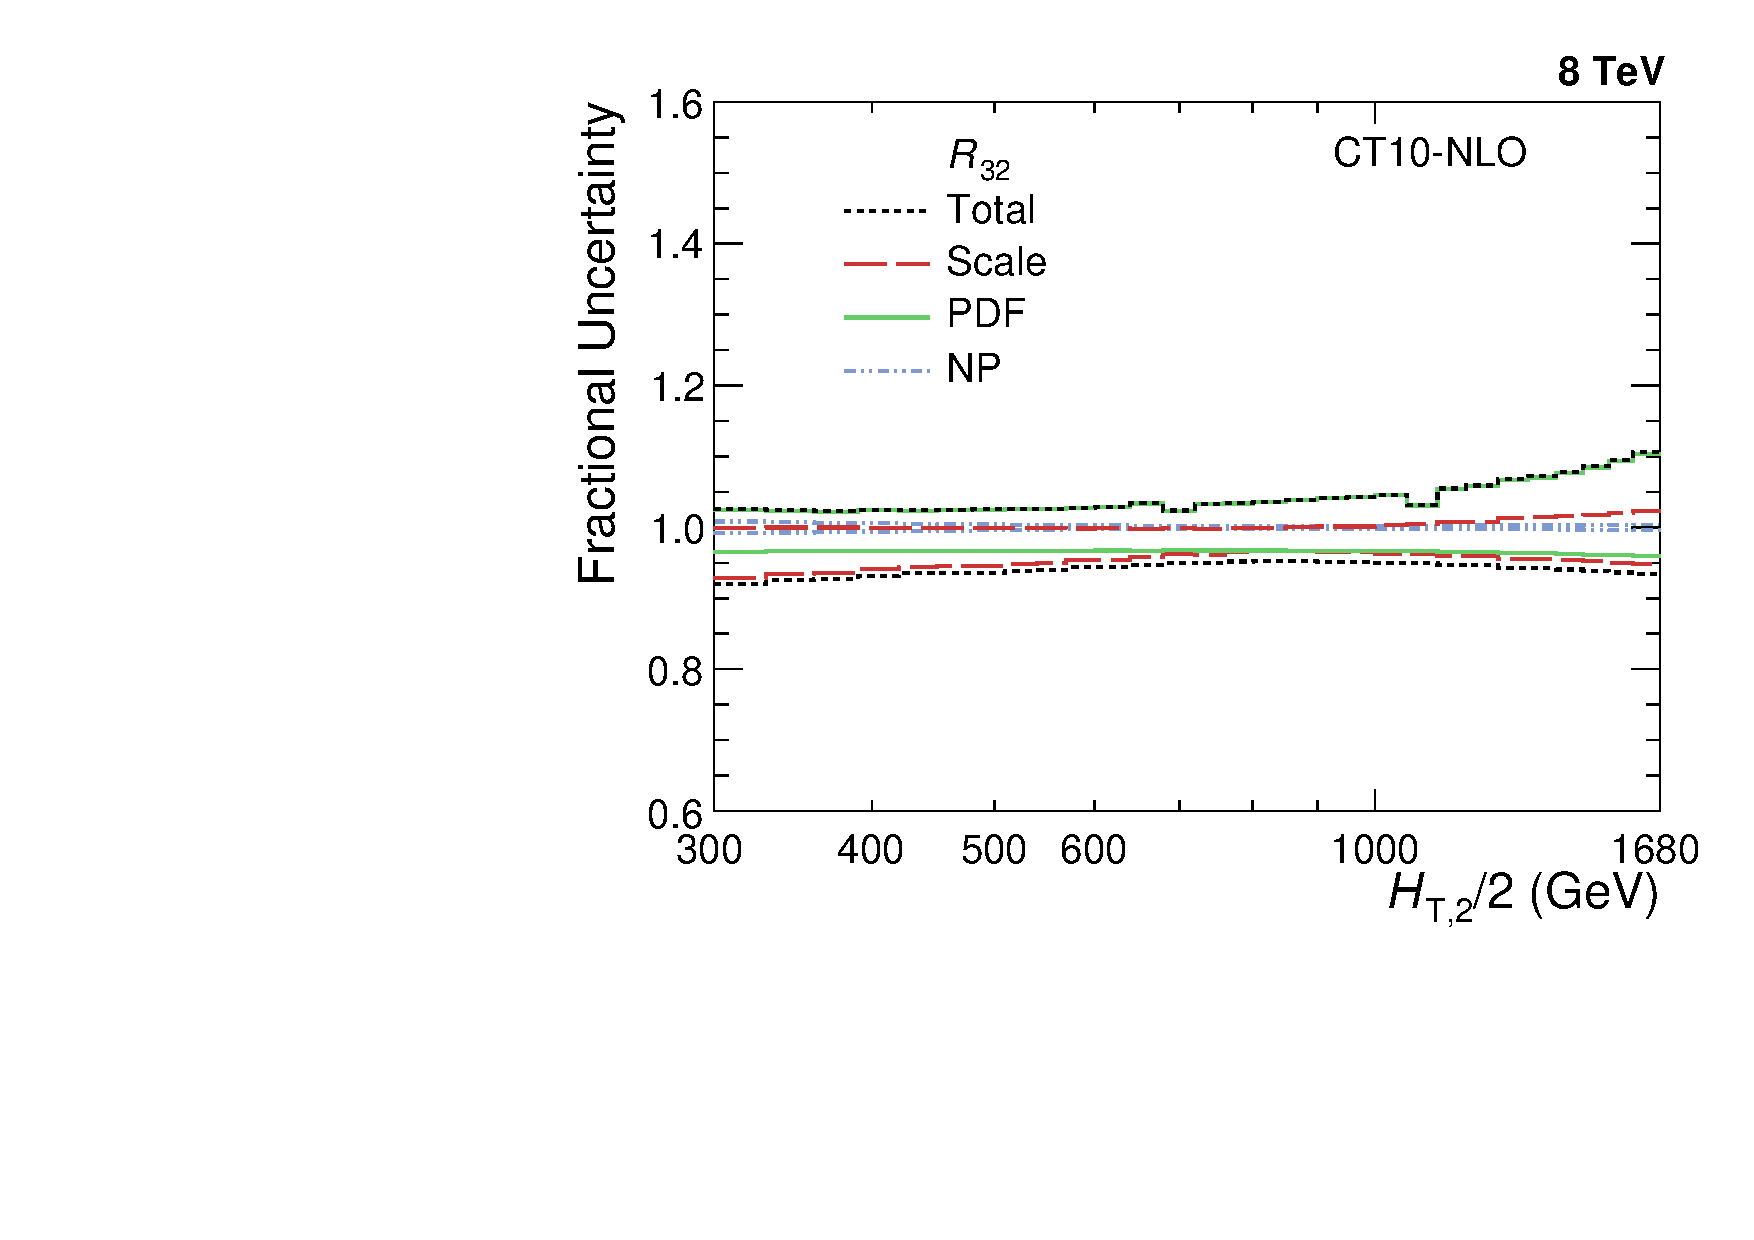
\includegraphics[scale = 0.25]{/home/anter/Desktop/Analysis_8/Present_Latex/Approval/Approval_New/Theory_Unc_Ratio_32.pdf}\\
\end{minipage}
\vspace{-10mm}
\begin{itemize}
\item \tiny {\green {Small dips at 1.X TeV in the PDF uncertainty (top right) : \\ It is a feature of the CT10 PDF. Likewise the smaller dip at 700 GeV. \\ If another PDF, e.g. CT14, is used, these dips are gone (Slide no.~\ref{theory_unc} in Back-Up). } \\}
\end{itemize}
\end{frame}
\ball

%##################################### Slide : 21 ###########################################
\begin{frame}
\frametitle{\centerline{Inclusive Differential Multijet Measurement}}
\setlength\labelsep   {\dimexpr\labelsep + 0.05em\relax}  
\setlength\leftmargini{\dimexpr\leftmargini + 0.05em\relax}
\begin{center}
\vspace{-3.2mm}
\begin{itemize}
\item {\scriptsize Inclusive  differential  multijet  cross  sections  are  measured  as  a  function  of  the  average transverse  momentum, \httwo \\ }
\tri
\begin{itemize}
\item {\scriptsize {\bf On Left :} NLOJet{\plus\plus} predictions based on the CT10 PDF set and corrected for NP effects, in addition for EWK effects in the 2-jet case \\}
\setbeamertemplate{itemize items}[circle]
\begin{itemize}
\item {\scriptsize predictions are compatible with data within uncertainties over a wide range of \httwo from 300 GeV up to 2 TeV \\ }
\end{itemize}
\tri
\item {\scriptsize {\bf On Right :} predictions from MG\plus P6 Z2*, corrected for EWK effects in the 2-jet case \\}
\setbeamertemplate{itemize items}[circle]
\begin{itemize}
\item {\scriptsize significant discrepancies are visible in the ratio for comparison with the leading-order (LO) tree-level prediction \\}
\end{itemize}
\end{itemize} 
\end{itemize}
\vspace{0.4mm}
%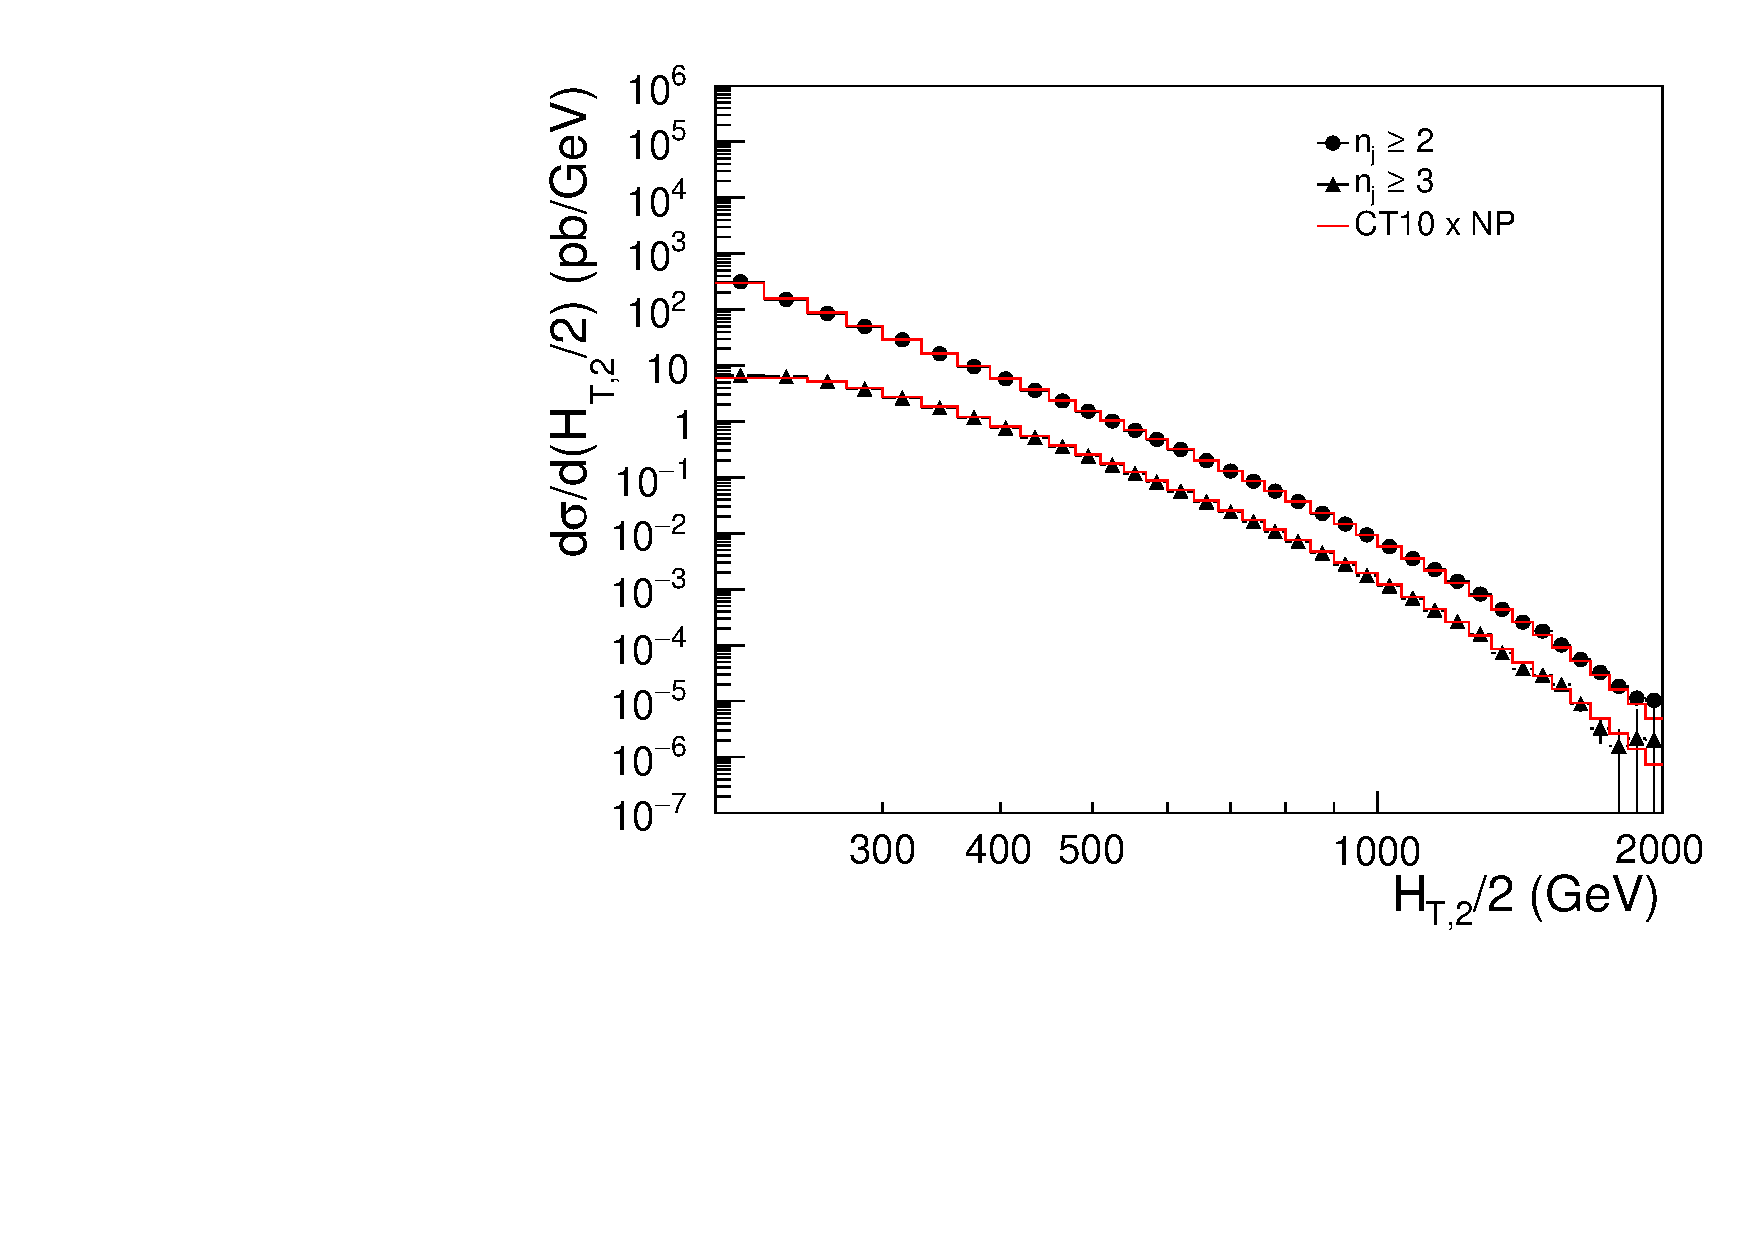
\includegraphics[scale = 0.20]{/home/anter/Desktop/Analysis_8/Present_Latex/After_Pre-approval/New_Plots_PAS/Comparison_data_theory.pdf}%
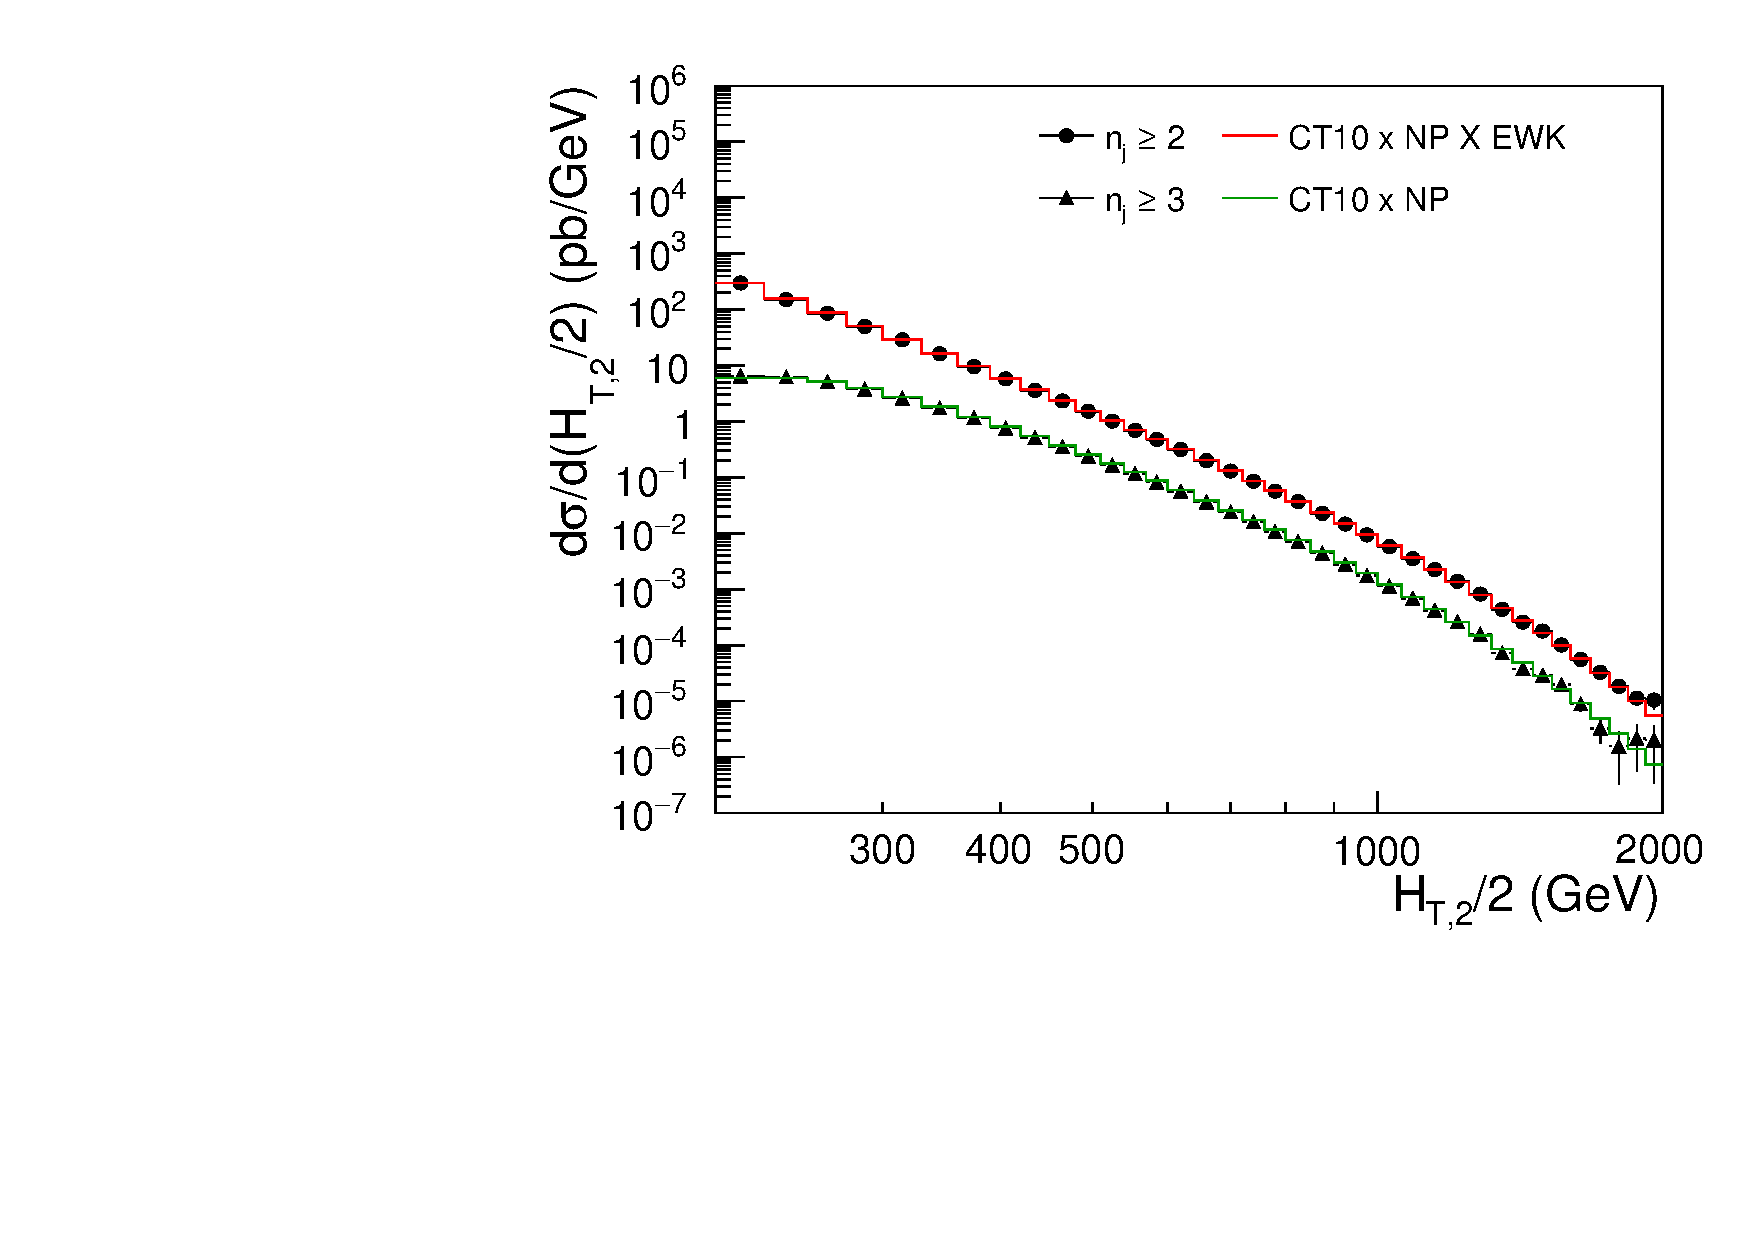
\includegraphics[scale = 0.28]{/home/anter/Desktop/Analysis_8/Present_Latex/Approval/Approval_New/Comparison_data_theory_EWK.pdf}%
\hspace{5mm}
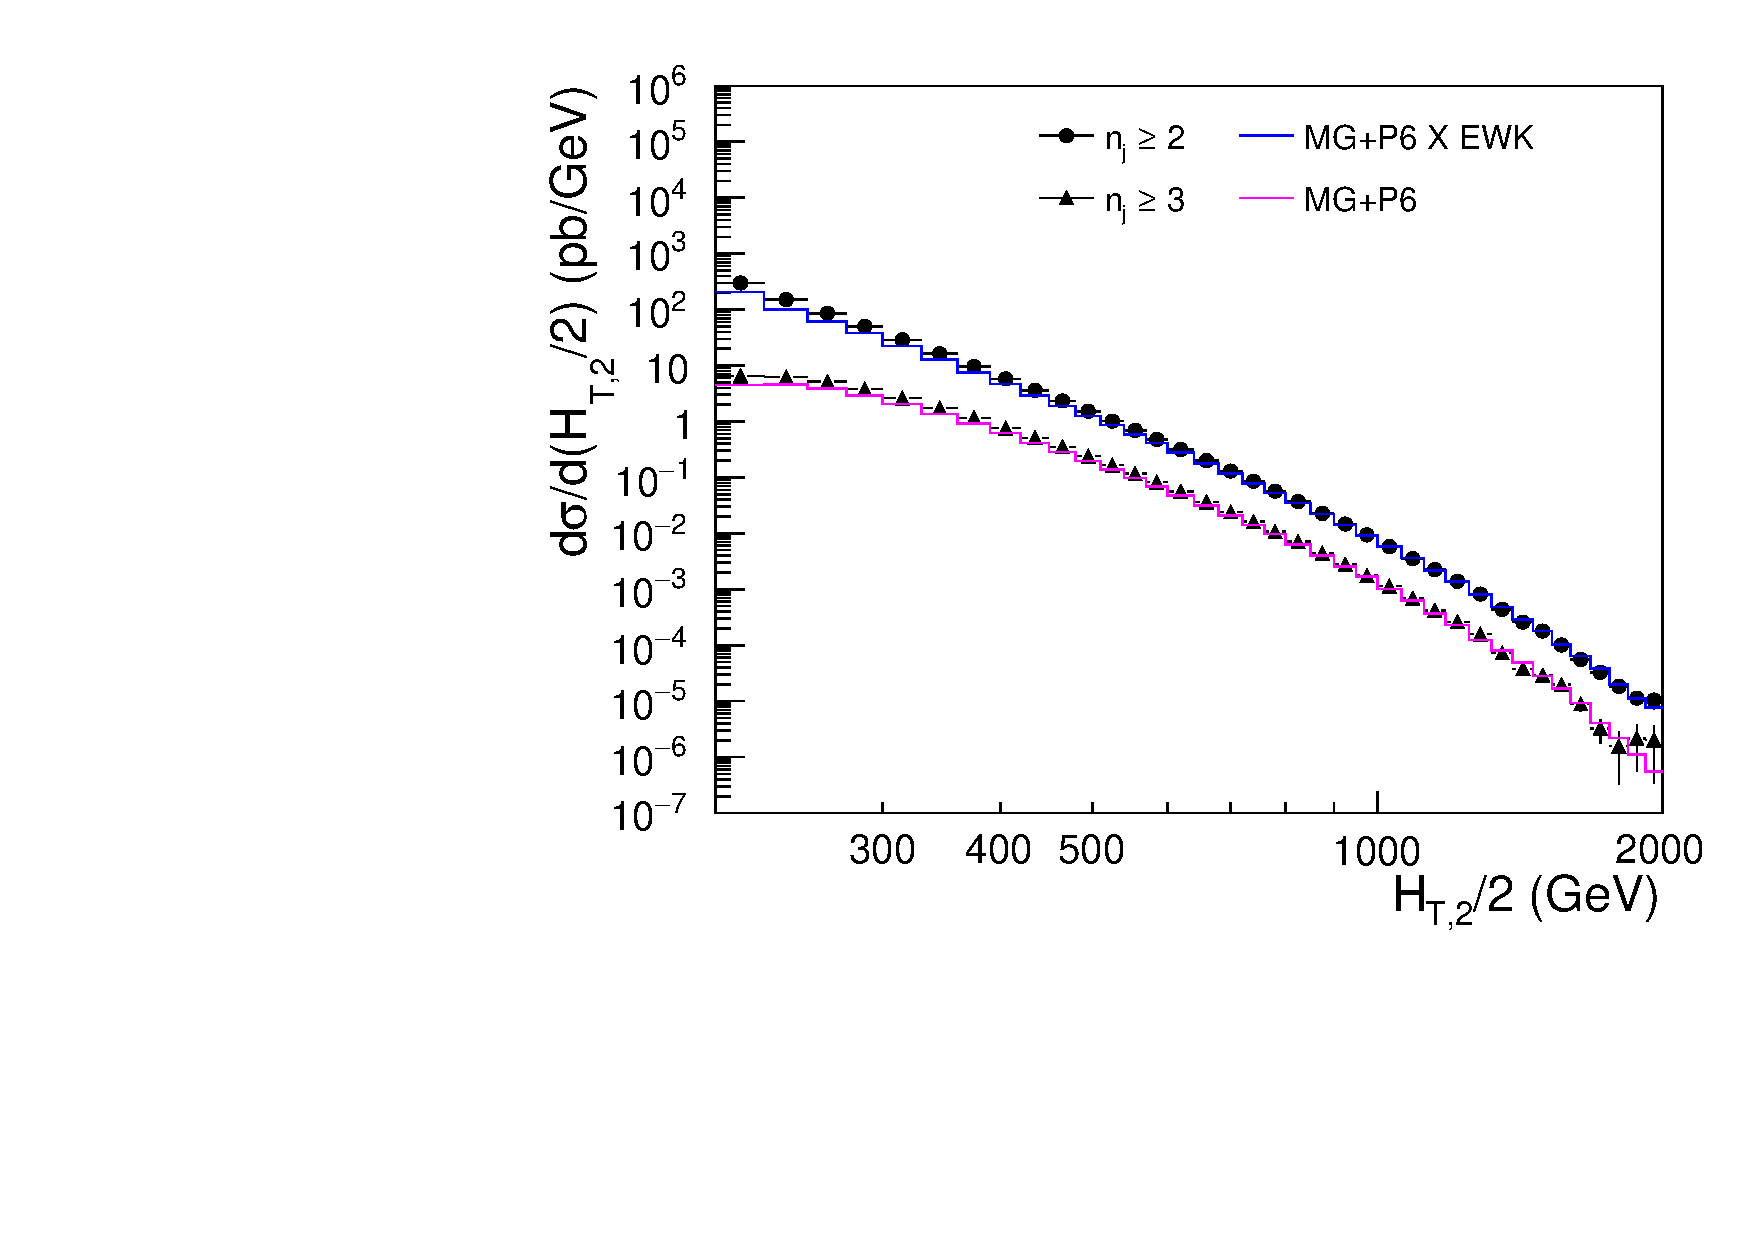
\includegraphics[scale = 0.28]{/home/anter/Desktop/Analysis_8/Present_Latex/Approval/Approval_New/Comparison_data_MC_EWK.pdf} \\

\end{center}
\end{frame}
\ball
%##################################### Slide : 22 ###########################################
\begin{frame}
\frametitle{\centerline{Comparison with NLO Predictions - CT10}}
\setlength\labelsep   {\dimexpr\labelsep + 0.05em\relax}  
\setlength\leftmargini{\dimexpr\leftmargini + 0.05em\relax}
\begin{center}
\vspace{-3.5mm}
\begin{itemize}
\item { \scriptsize Ratio to NLO$\otimes$NP$\otimes$EWK - CT10
\vspace{1mm}
\item {\bf Data points} with statistical uncertainty
\vspace{1mm}
\item \textcolor{airforceblue}{Theoretical uncertainty} : quad. sum of scale, NP and PDF uncertainties
\vspace{1mm}
\item \mycolor {Experimental uncertainty} shows total systematic uncertainty \\}
\end{itemize}
\vspace{-3mm}
\end{center}
\vspace{-2.5mm}
\hspace{-5.3mm}
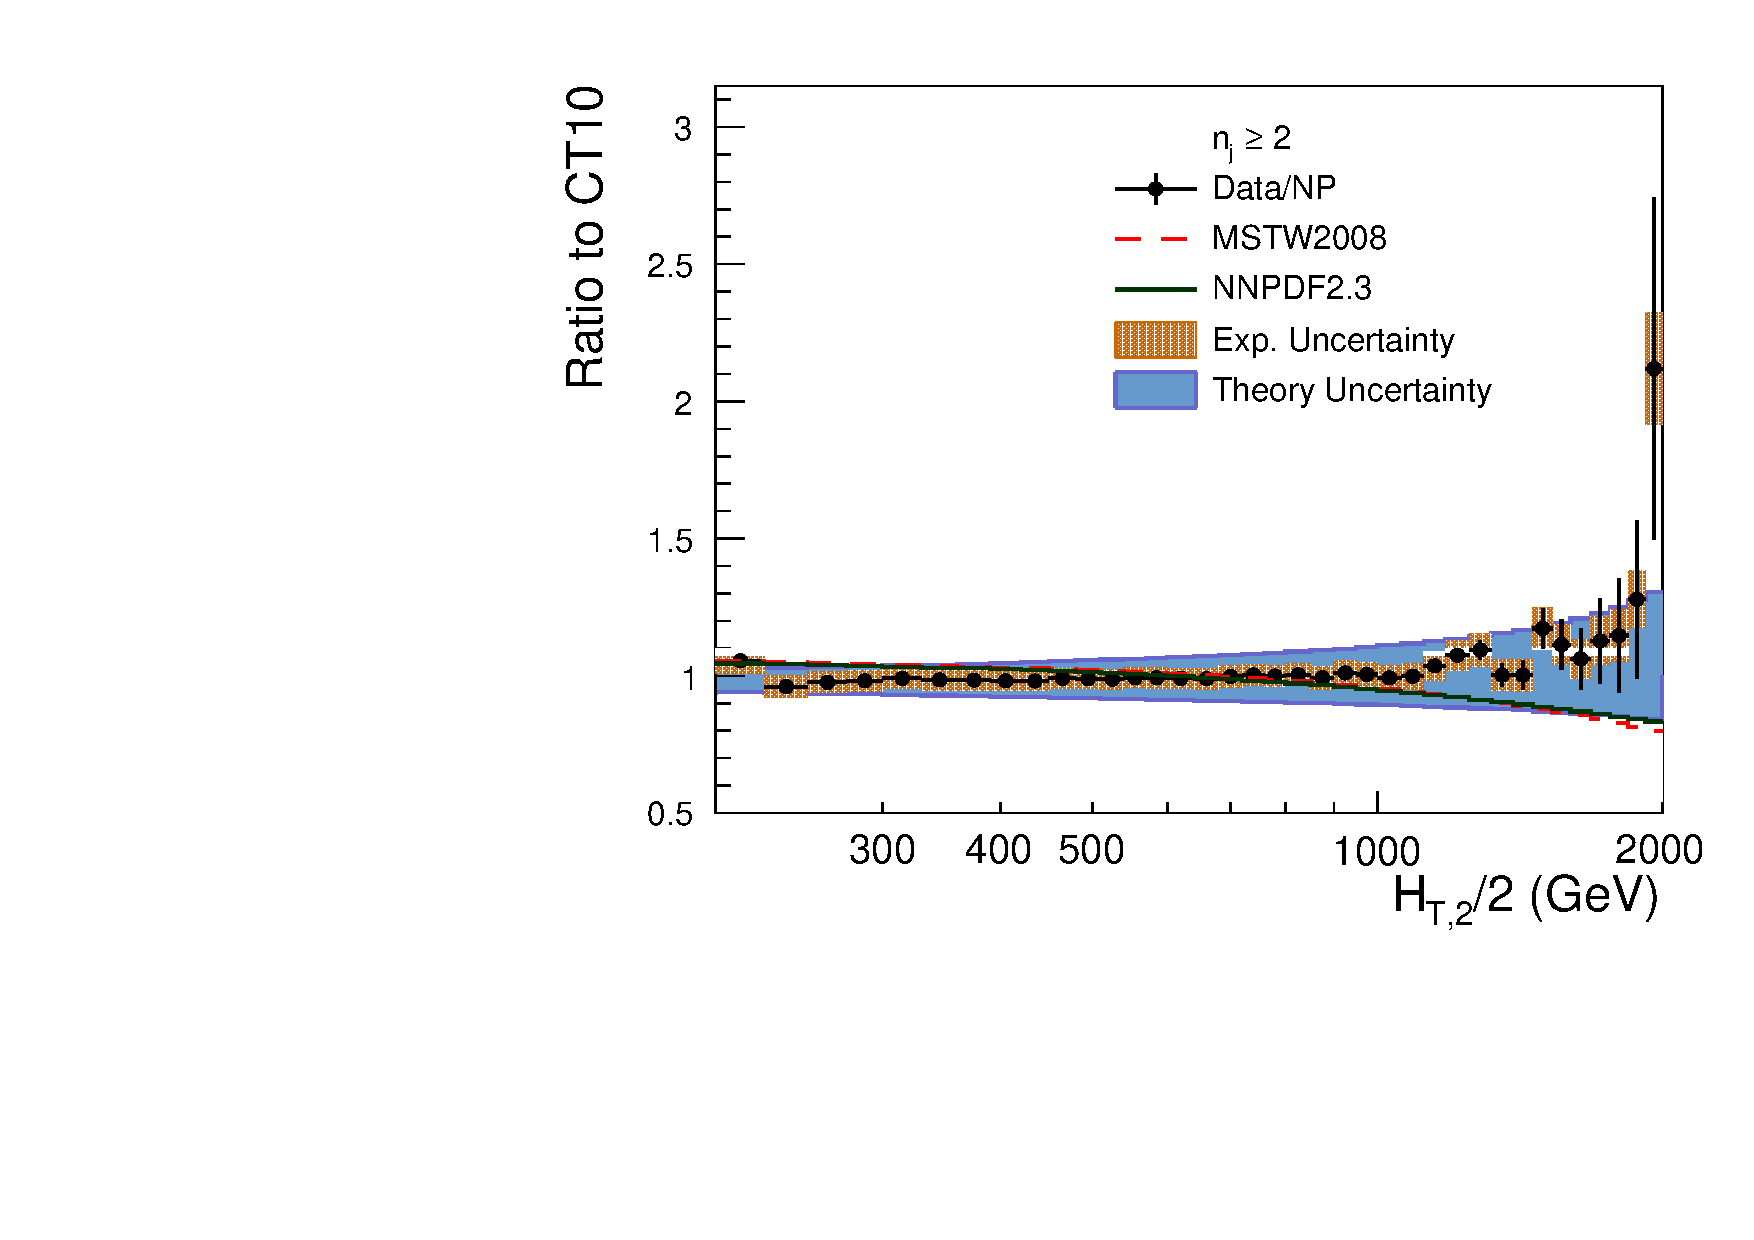
\includegraphics[scale = 0.215]{/home/anter/Desktop/Analysis_8/Present_Latex/Approval/Approval/Comparison_data_NLO_Pdfs_2.pdf}%
\includegraphics[scale = 0.215]{/home/anter/Desktop/Analysis_8/Present_Latex/Approval/Approval_New/Comparison_data_NLO_Pdfs_2_EW_box.pdf}%
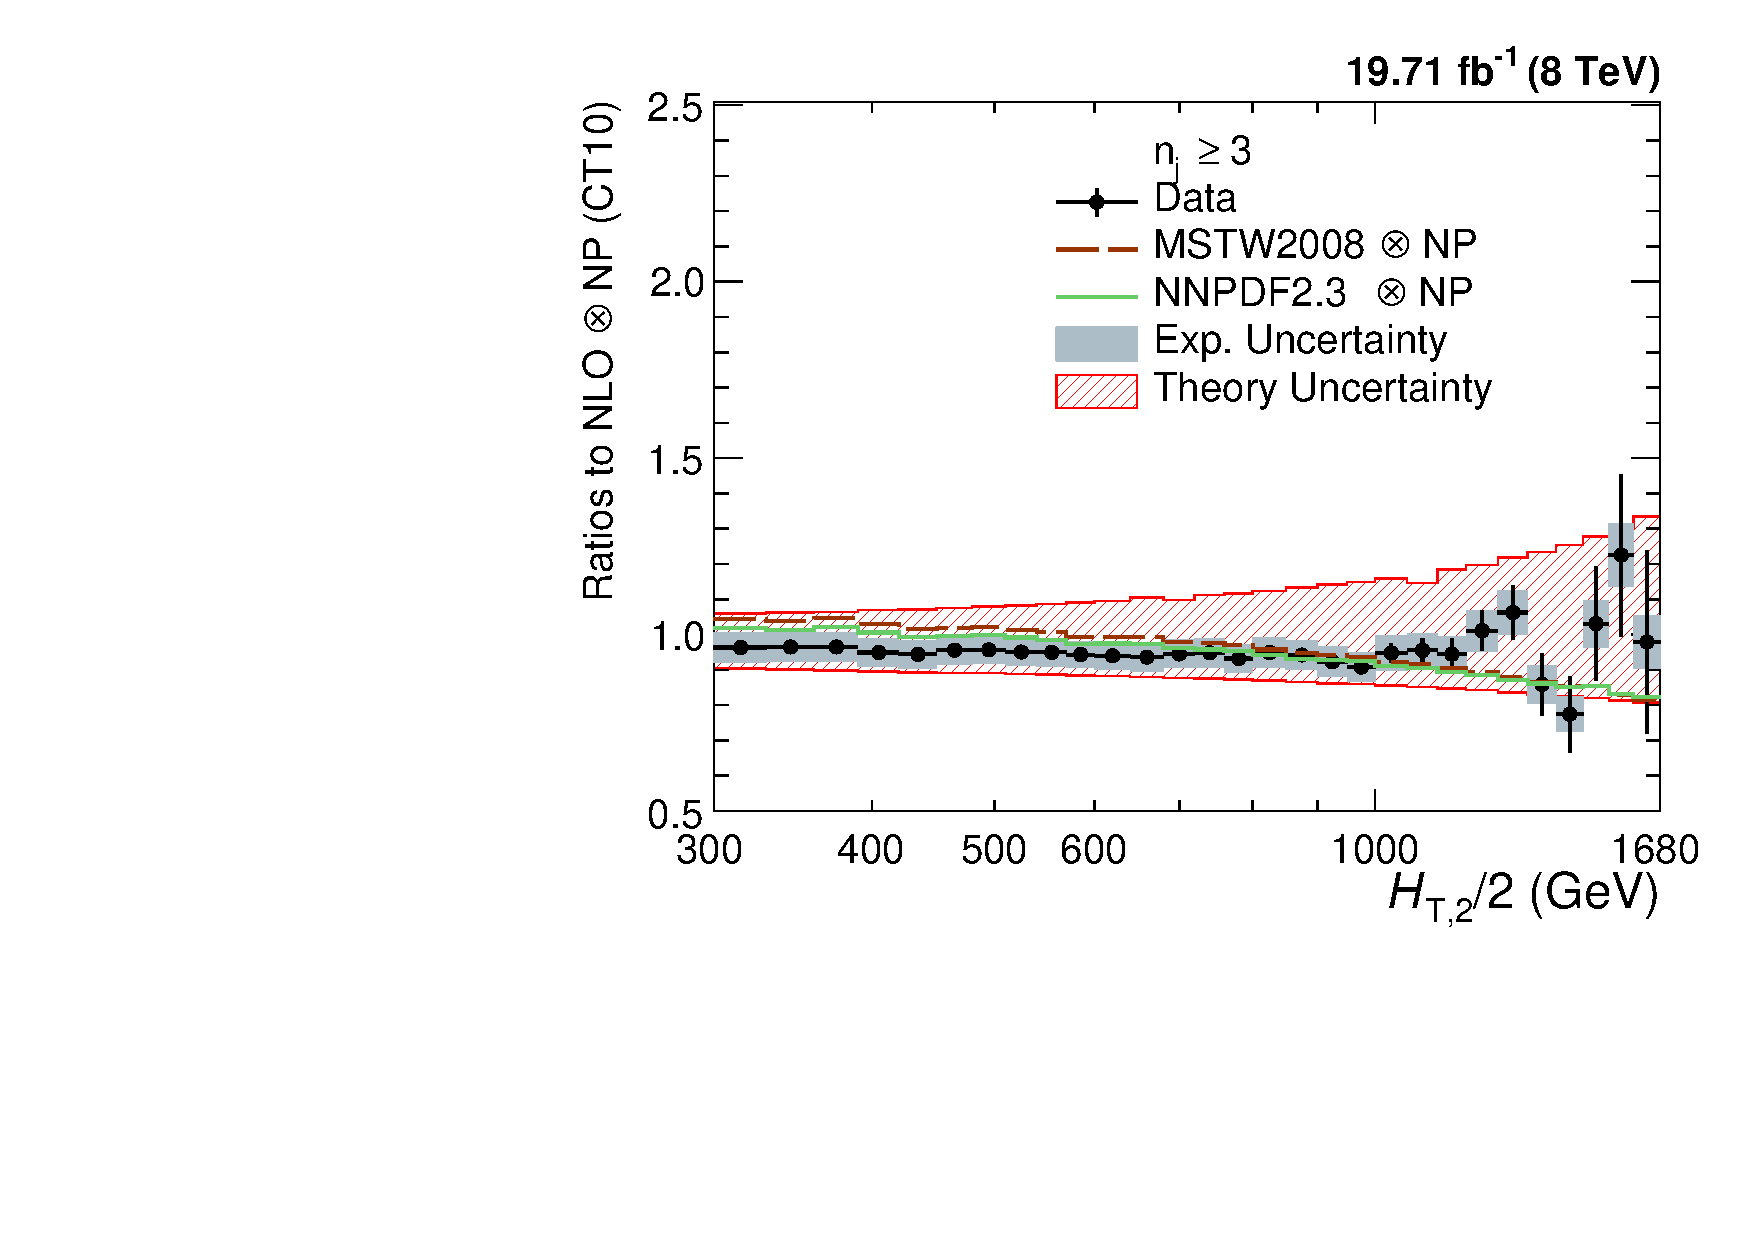
\includegraphics[scale = 0.215]{/home/anter/Desktop/Analysis_8/Present_Latex/Approval/Approval_New/Comparison_data_NLO_Pdfs_3.pdf}
\hspace{-4mm}
\begin{minipage}[tbp]{0.3\textwidth}
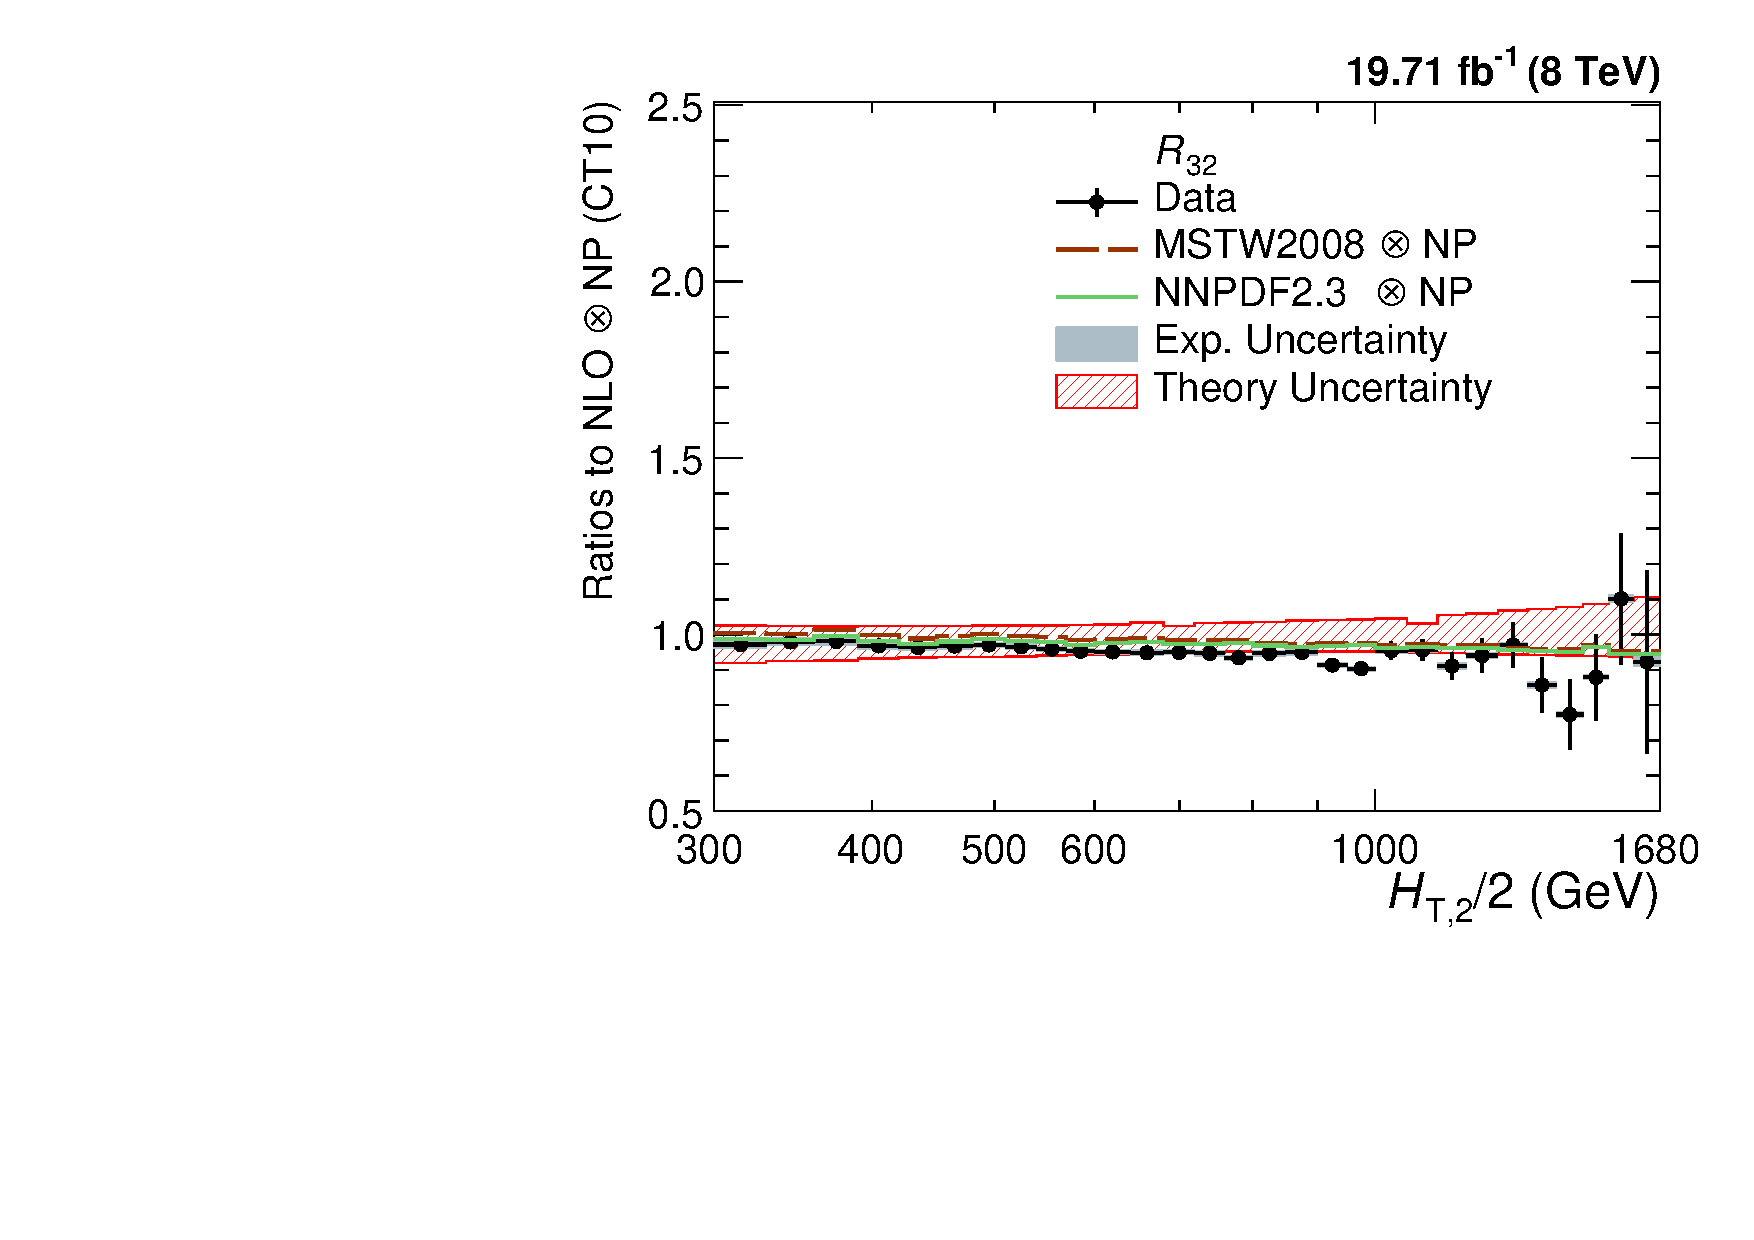
\includegraphics[scale = 0.22]{/home/anter/Desktop/Analysis_8/Present_Latex/Approval/Approval_New/Comparison_data_NLO_Pdfs_ratio_32.pdf}
\end{minipage}
\hspace{7mm}
\begin{minipage}[tbp]{0.6\textwidth}
\begin{itemize}
\item {\scriptsize \green{Electroweak corrections explain the increasing systematic excess of data with respect to theory beyond 1 TeV of \httwo for inclusive 2-jet (Left and Middle figures)} 
\vspace{1mm}
\item For brevity, the relative factor of NP between data and theory has been indicated
as “Data/NP” in the legend \\ }
%\vspace{1mm}
%\item Some dips (2 bins) in between 1 TeV and 2 TeV (left plot) : Statistical feature already present in the detector level data for both, 2-jet and 3-jet events. The points are compatible within statistical uncertainty.}
\end{itemize}
\end{minipage}
%\hspace{-7mm}
%\end{center}
\end{frame}

%##################################### Slide : 23 ###########################################
\begin{frame}
\frametitle{\centerline{Comparison with MC Generators}}
\setlength\labelsep   {\dimexpr\labelsep + 0.05em\relax}
\setlength\leftmargini{\dimexpr\leftmargini + 0.05em\relax}
\begin{center}
\vspace{-1mm}
\begin{itemize}
\item { \scriptsize Ratios to \green{Powheg\plus Pythia8 tune CUETS1}
\vspace{0.5mm}
\item {\bf Data points} with statistical uncertainty
\vspace{0.5mm}
\item \textcolor{brown}{Experimental uncertainty} shows total systematic uncertainty
\vspace{0.5mm}
\item Comparison with \\}
\tri 
\begin{itemize}
\item {\scriptsize LO prediction from \blue{MG\plus P6 Z2*} and tree-level multi-leg improved prediction by \green{Pythia6 Z2*} : Significant discrepancies, which are cancelled to a large extent in the ratio \rations, are visible in particular for small \httwo 
\item with the matched dijet NLO prediction from \textcolor{grey}{Powheg\plus Pythia8 with tune CUETM1} : better describes the 2-jet event cross section, but fails for the 3-jet case. \\}
\end{itemize}
\ball
\end{itemize}
\end{center}
\hspace{-5mm}
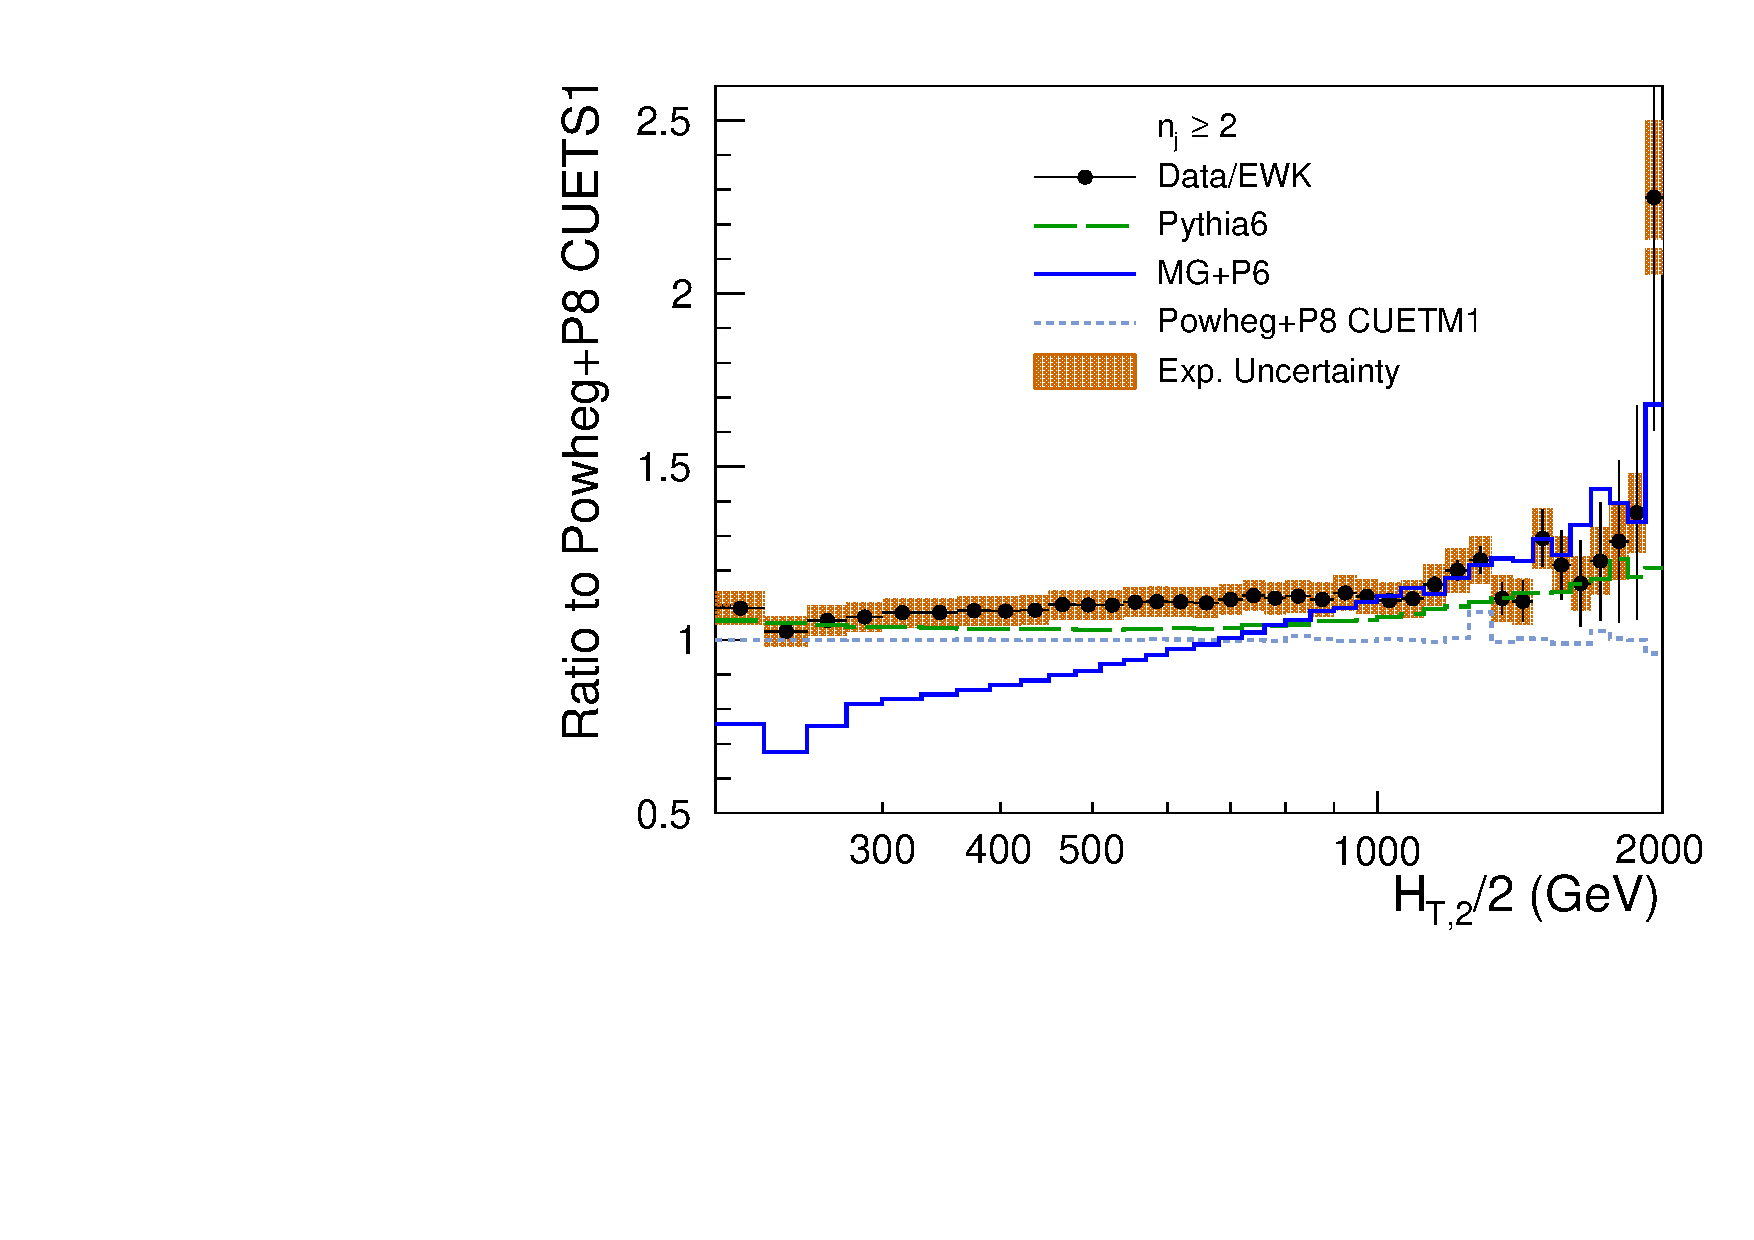
\includegraphics[scale = 0.215]{/home/anter/Desktop/Analysis_8/Present_Latex/Approval/Approval_New/Comparison_data_MC_samples_2_Pow_EWK.pdf}%
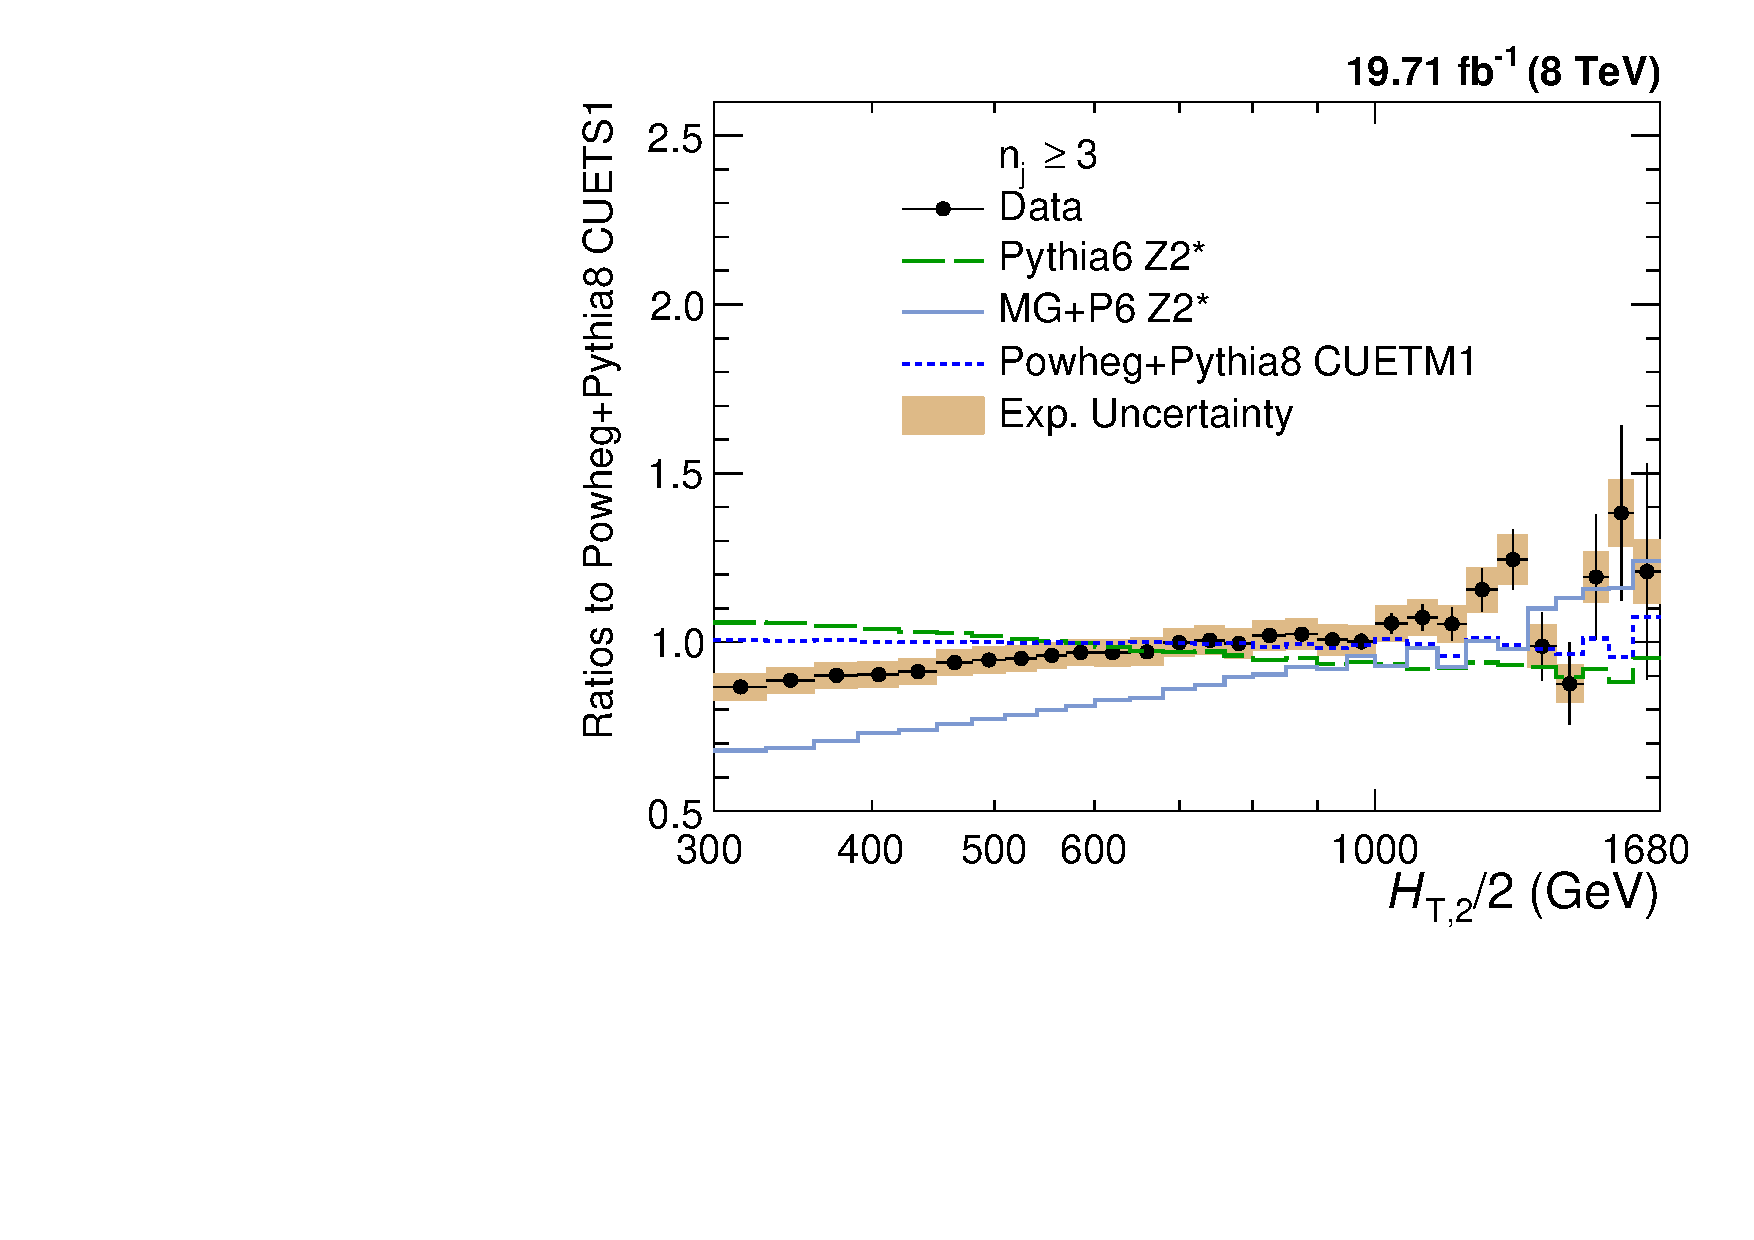
\includegraphics[scale = 0.215]{/home/anter/Desktop/Analysis_8/Present_Latex/Approval/Approval_New/Comparison_data_MC_samples_3_Pow.pdf}%
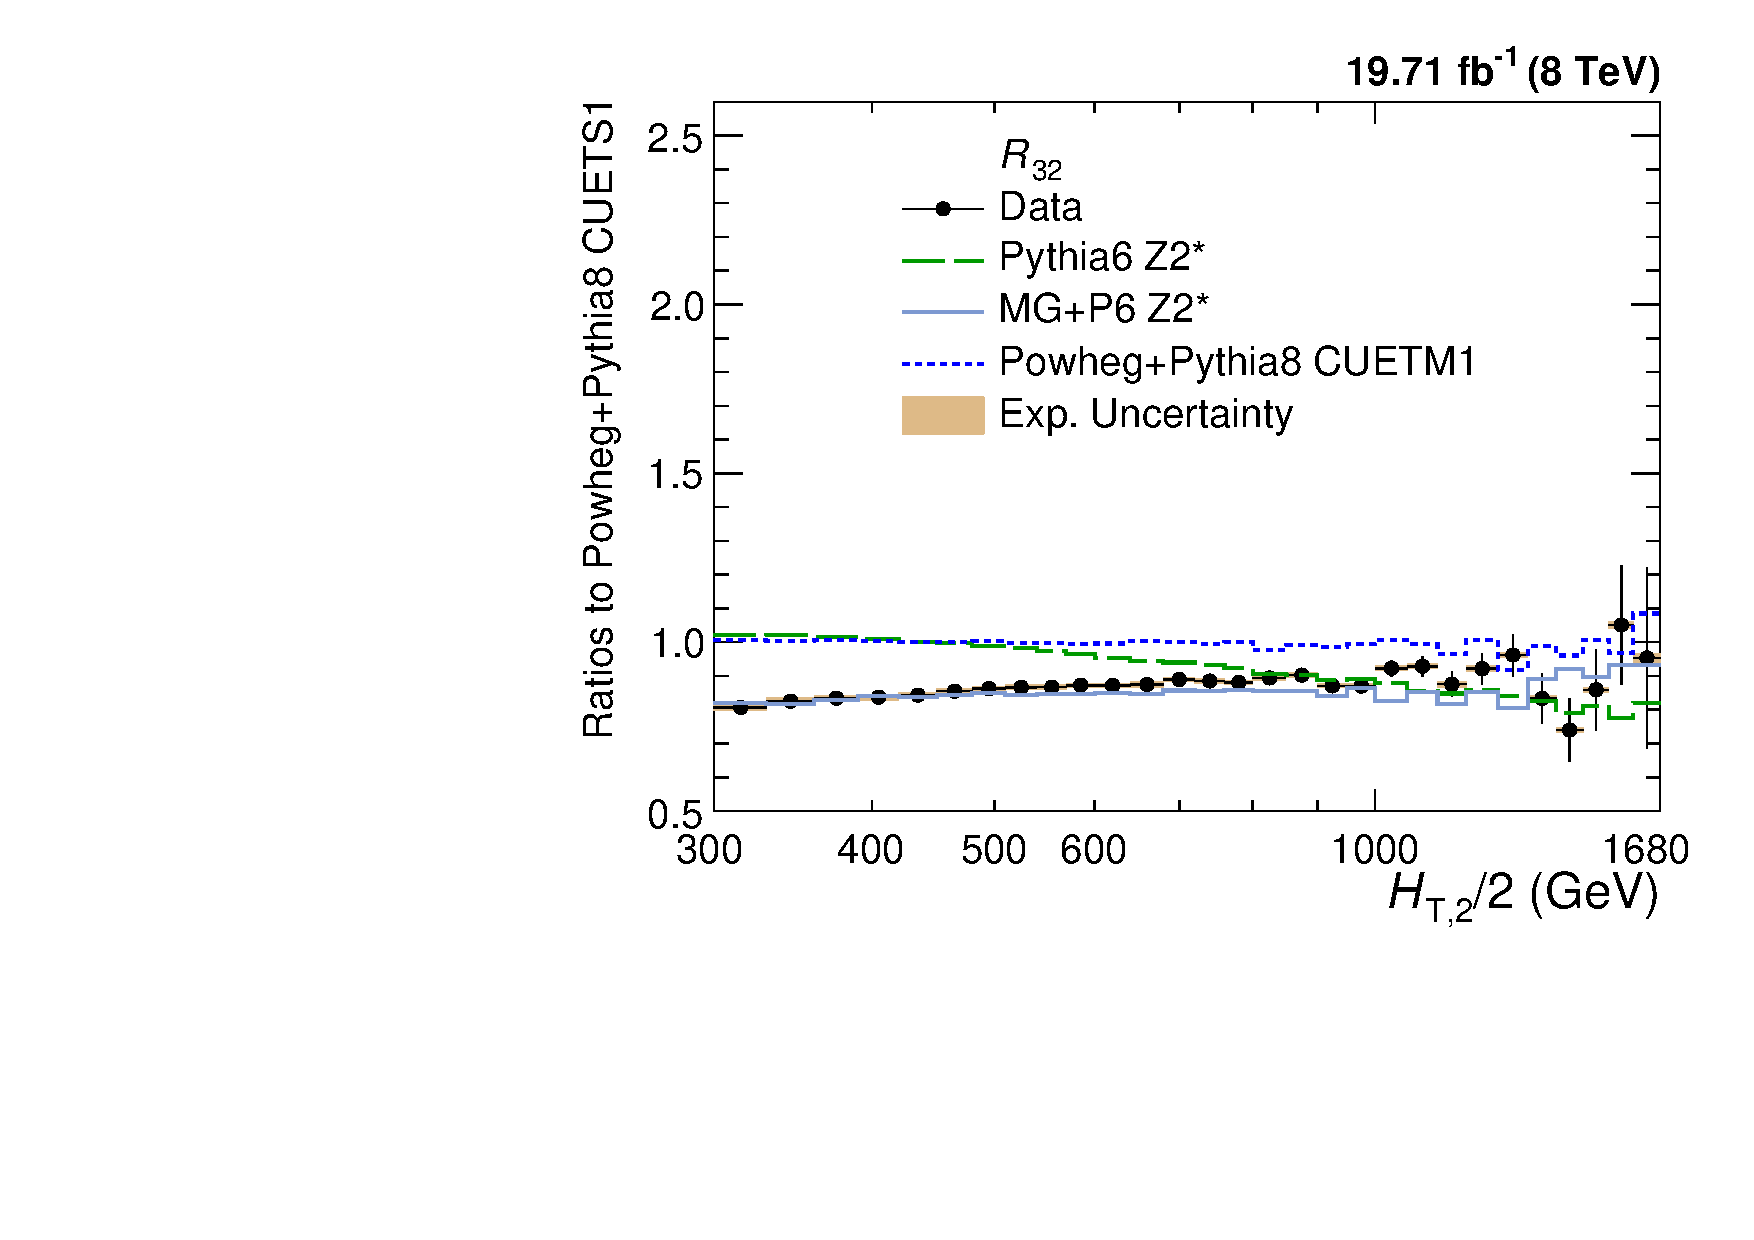
\includegraphics[scale = 0.215]{/home/anter/Desktop/Analysis_8/Present_Latex/Approval/Approval_New/Comparison_data_MC_samples_ratio_32_Pow.pdf}
\end{frame}

%##################################### Slide : 24 ###########################################
\begin{frame}
\frametitle{\centerline{Cross section ratio (\rations)}}
\setlength\labelsep   {\dimexpr\labelsep + 0.05em\relax}
\setlength\leftmargini{\dimexpr\leftmargini + 0.05em\relax}
\begin{center}
\vspace{-4mm}
\begin{itemize}
\item { \scriptsize The cross-section ratio \ratio as a function of \httwo is extracted by dividing the differential cross section for inclusive 3-jet over 2-jet events for each bin in \httwo \\ }
\vspace{-6mm}
\begin{align*} 
\resizebox{.20\hsize}{!}{$\rm R_{32} = \frac{\sigma_{3\mbox{-}jet}}{\sigma_{2\mbox{-}jet}}$ $\propto$ $\alps$}
\end{align*}
\vspace{-5mm}
\item { \scriptsize \ratio obtained from unfolded data in comparison to that from CT10 NLO \green{with NP corrections}. The error bars correspond to the total
experimental uncertainty. \\}
\end{itemize}
\vspace{2mm}
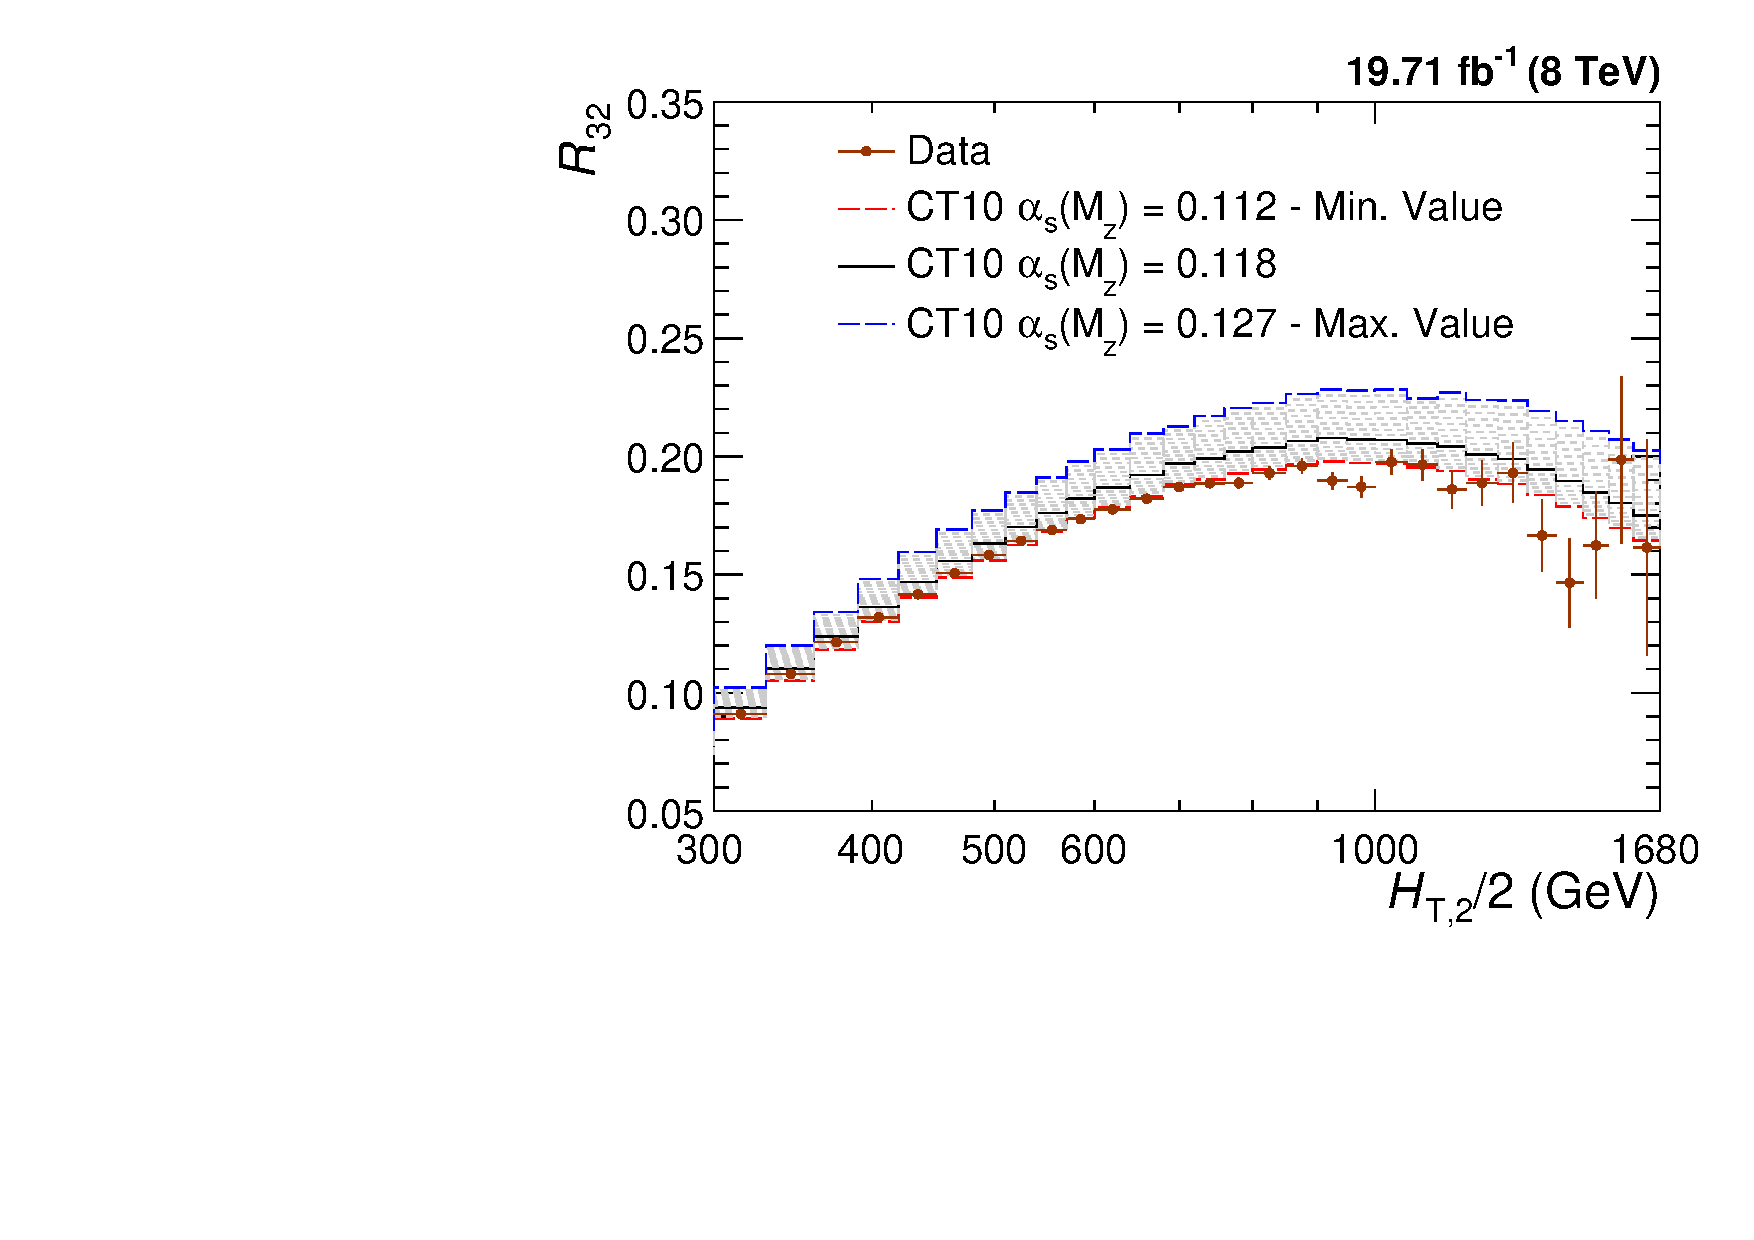
\includegraphics[scale = 0.30]{/home/anter/Desktop/Analysis_8/Present_Latex/Approval/Approval_New/Sensitivity/Sensitivity_ratio_32_CT10.pdf}
\begin{itemize}
\item { \scriptsize The other ratios will also be included once the theory predictions for inclusive 4-jet events are available (for Paper). \\}
\end{itemize}
\end{center}
\end{frame}

%##################################### Slide : 25 ###########################################
\begin{frame}
\frametitle{\centerline{Sensitivity of differential inclusive 2-jet cross section to \alpsmz}}
\setlength\labelsep   {\dimexpr\labelsep + 0.05em\relax}
\setlength\leftmargini{\dimexpr\leftmargini + 0.05em\relax}
\begin{center}
\begin{itemize}
\item { \scriptsize $\rm {\sigma_{2\mbox{-}jet} \propto \alpsns^2}$ \\}
\end{itemize}
\vspace{5mm}
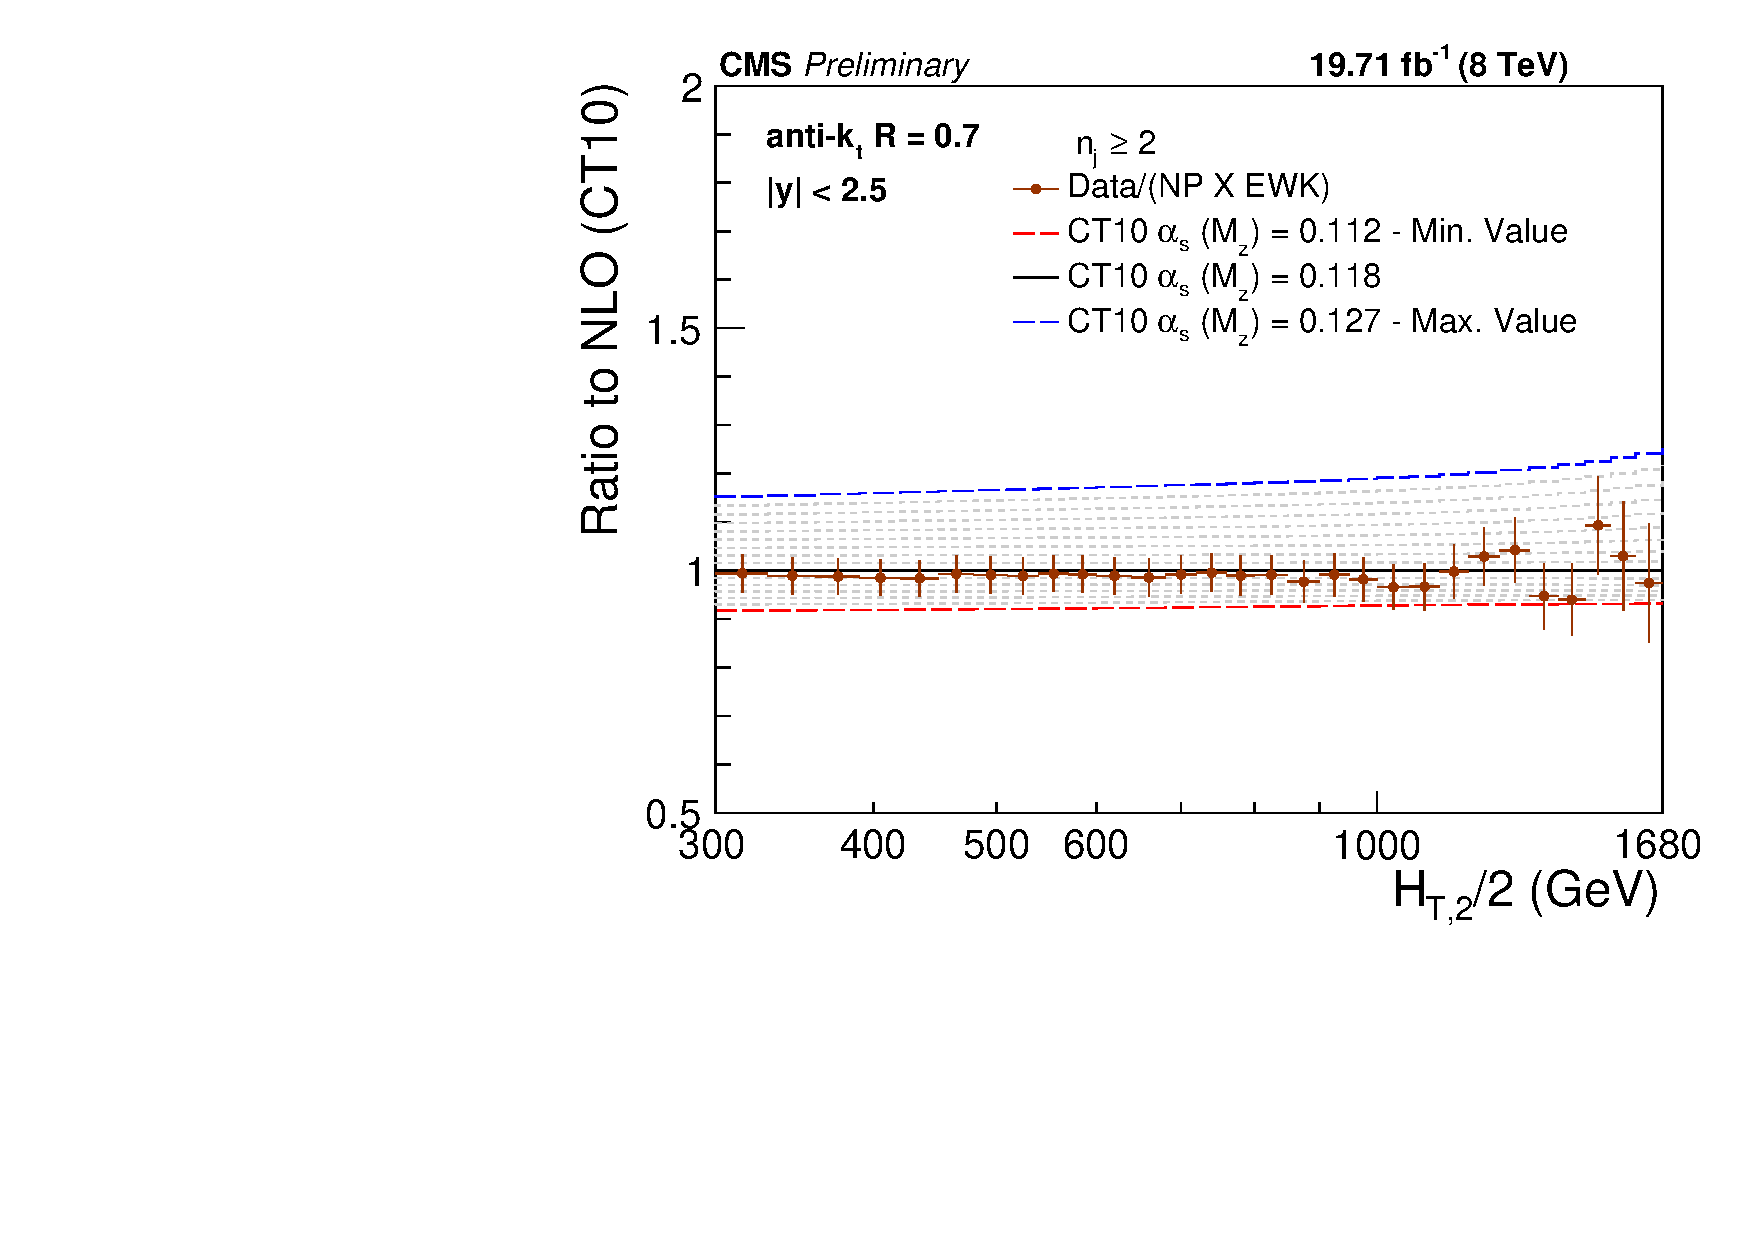
\includegraphics[scale = 0.207]{/home/anter/Desktop/Analysis_8/Present_Latex/Approval/Approval_New/Sensitivity/Sensitivity_2_ratio_NLO_CT10_EW.pdf}%
    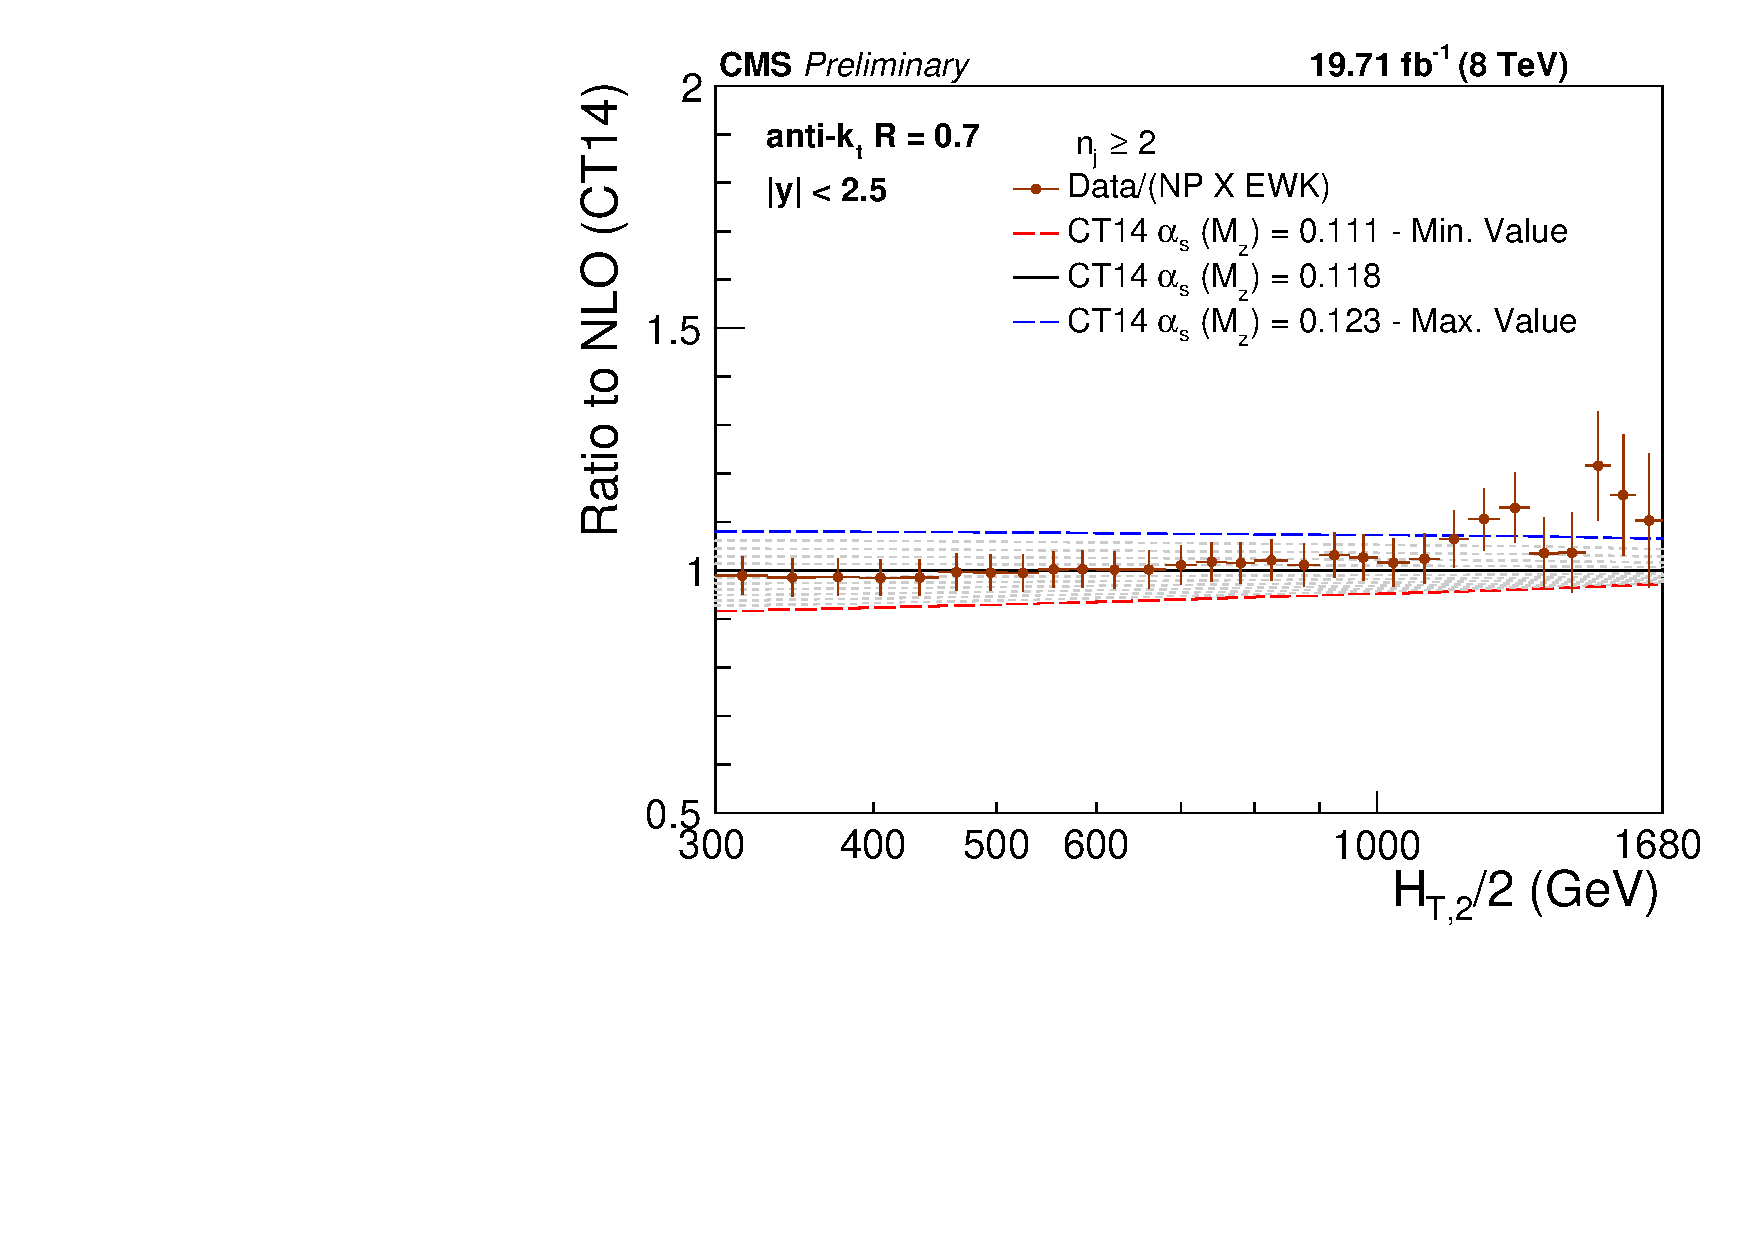
\includegraphics[scale = 0.207]{/home/anter/Desktop/Analysis_8/Present_Latex/Approval/Approval_New/Sensitivity/Sensitivity_2_ratio_NLO_CT14_EW.pdf}%
    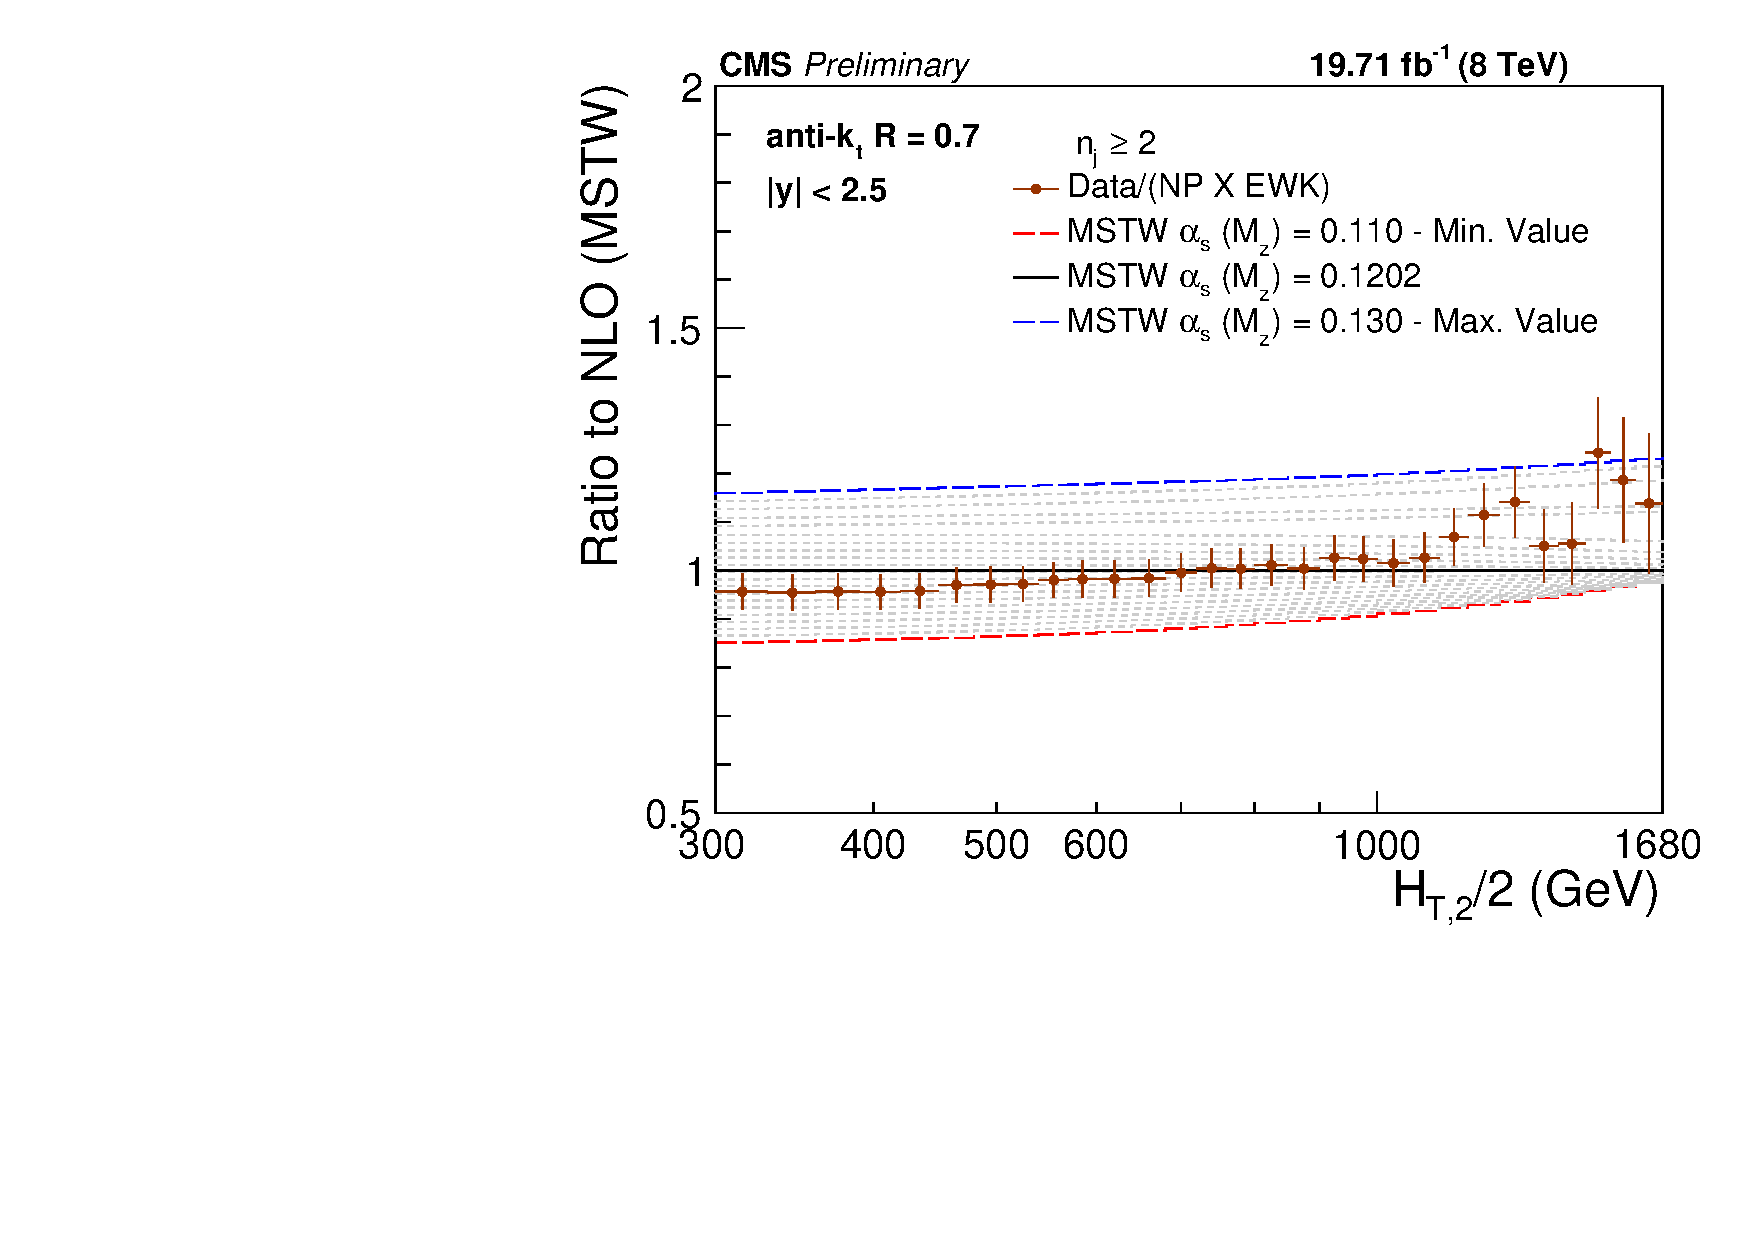
\includegraphics[scale = 0.207]{/home/anter/Desktop/Analysis_8/Present_Latex/Approval/Approval_New/Sensitivity/Sensitivity_2_ratio_NLO_MSTW2008_EW.pdf}\\
    \vspace{5mm}
    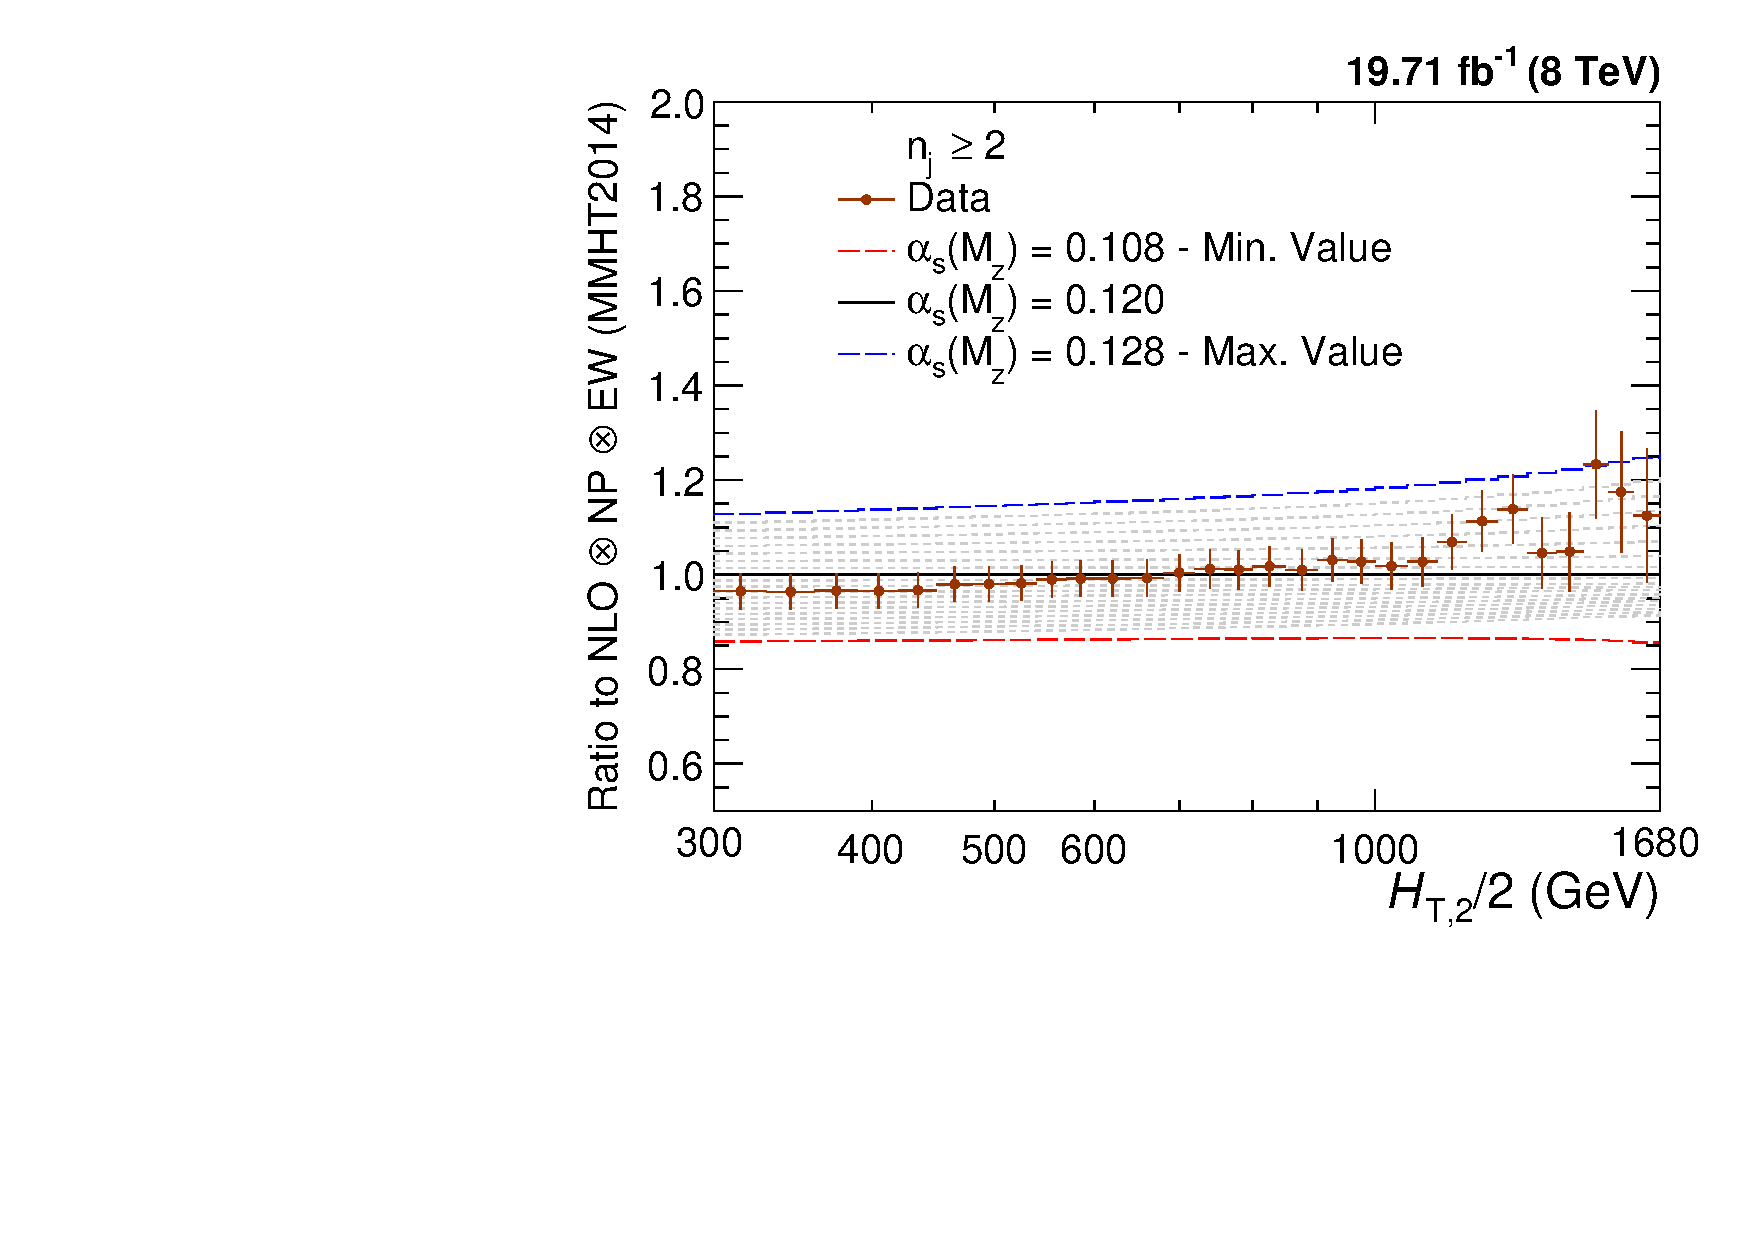
\includegraphics[scale = 0.207]{/home/anter/Desktop/Analysis_8/Present_Latex/Approval/Approval_New/Sensitivity/Sensitivity_2_ratio_NLO_MMHT2014_EW.pdf}%
    \hspace{0.3mm}
    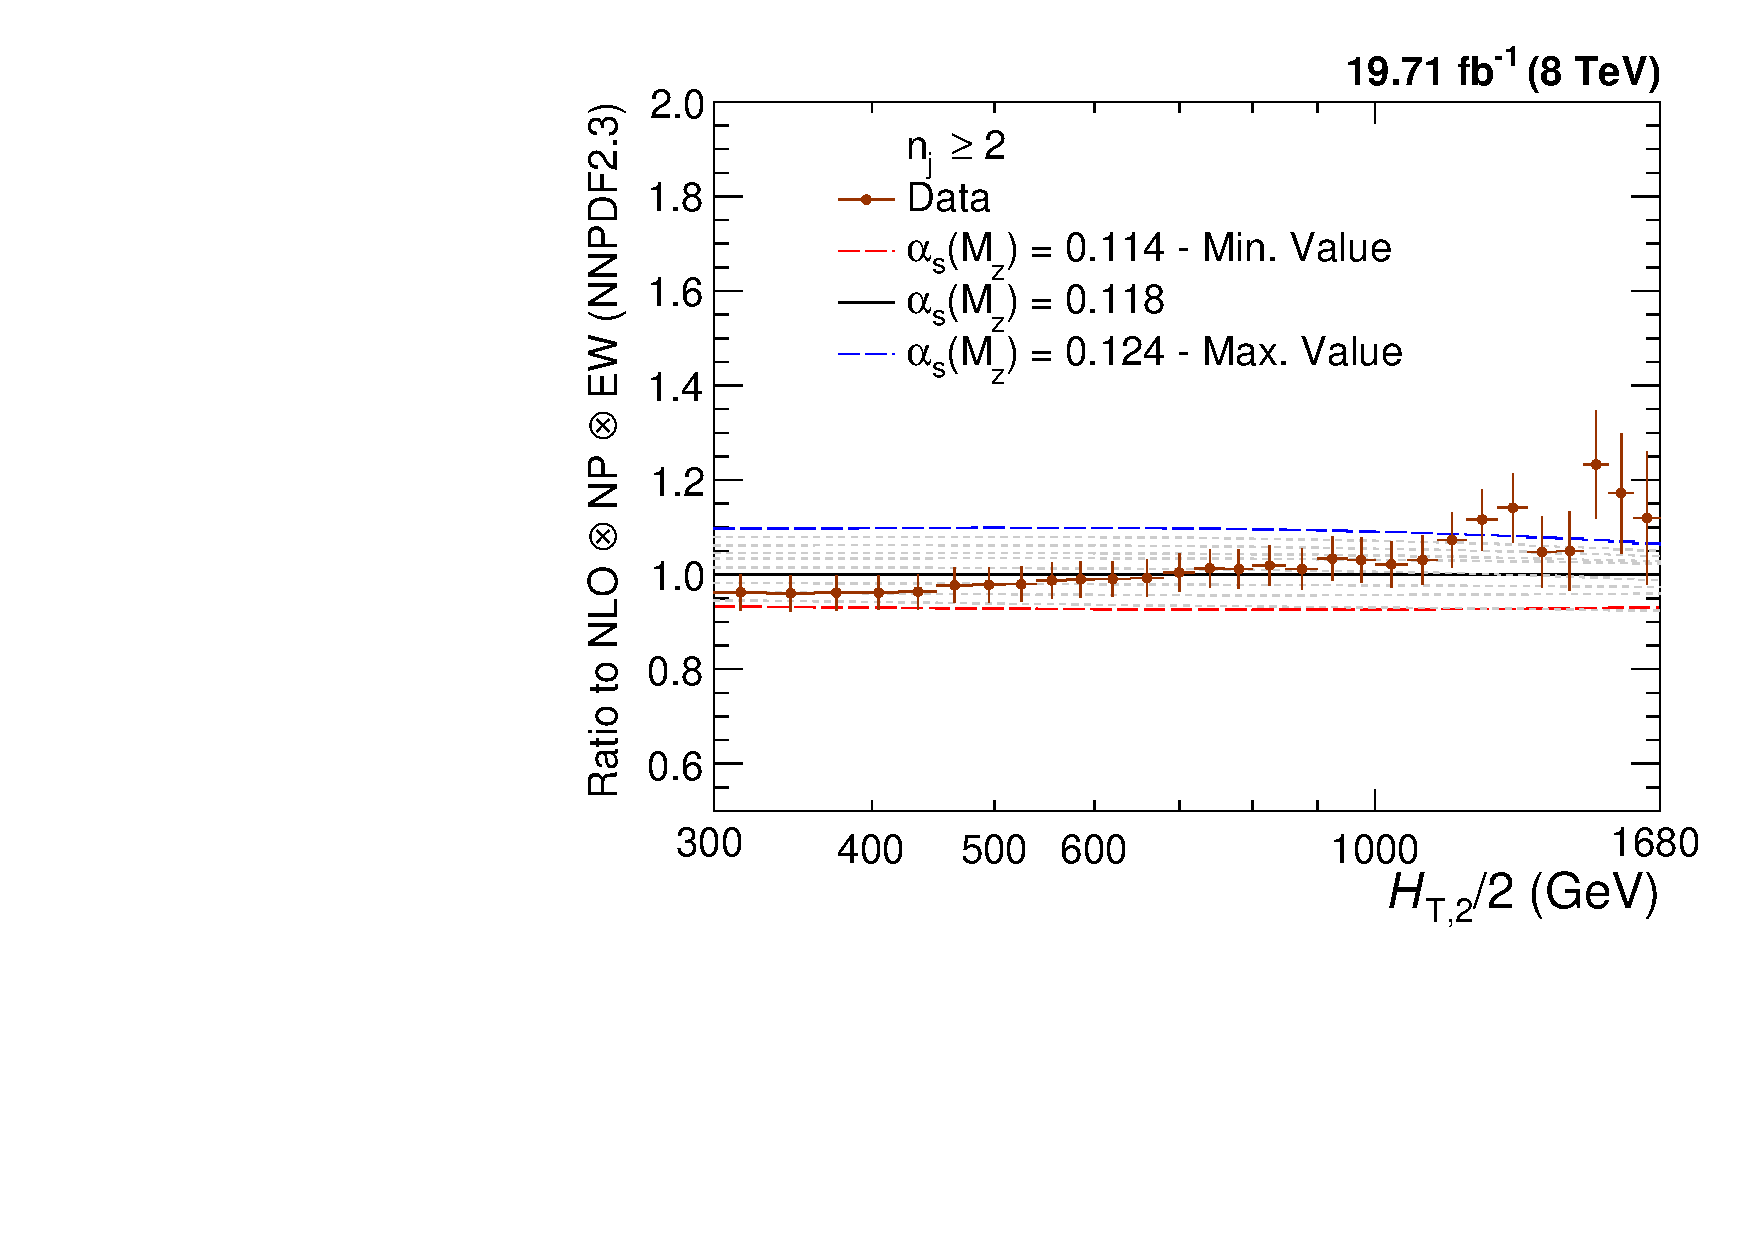
\includegraphics[scale = 0.207]{/home/anter/Desktop/Analysis_8/Present_Latex/Approval/Approval_New/Sensitivity/Sensitivity_2_ratio_NLO_NNPDF23_EW.pdf}
\end{center}
\end{frame}

%##################################### Slide : 26 ###########################################
\begin{frame}
\frametitle{\centerline{Sensitivity of differential inclusive 3-jet cross section to \alpsmz}}
\setlength\labelsep   {\dimexpr\labelsep + 0.05em\relax}
\setlength\leftmargini{\dimexpr\leftmargini + 0.05em\relax}
\begin{center}
\begin{itemize}
\item { \scriptsize $\rm {\sigma_{3\mbox{-}jet} \propto \alpsns^3}$ \\}
\end{itemize}
\vspace{5mm}
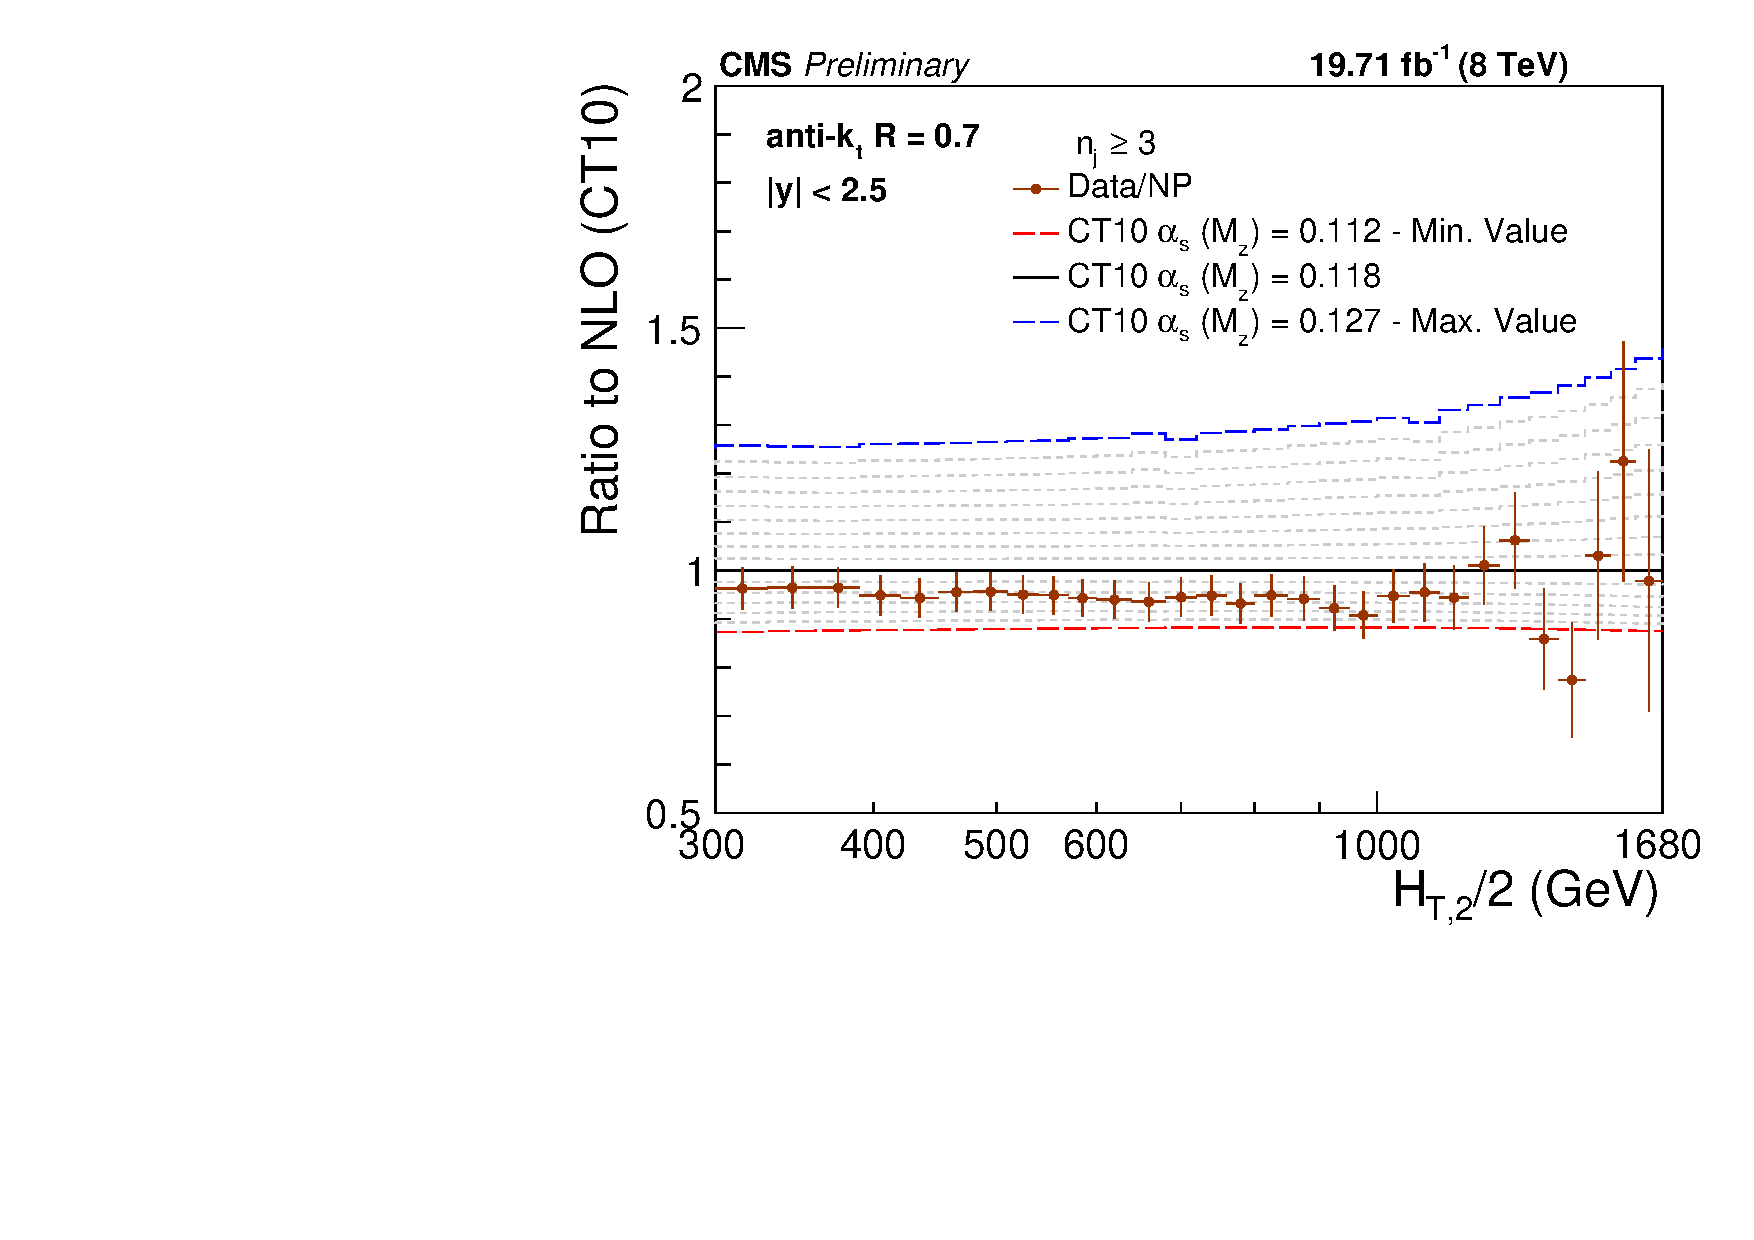
\includegraphics[scale = 0.207]{/home/anter/Desktop/Analysis_8/Present_Latex/Approval/Approval_New/Sensitivity/Sensitivity_3_ratio_NLO_CT10.pdf}%
    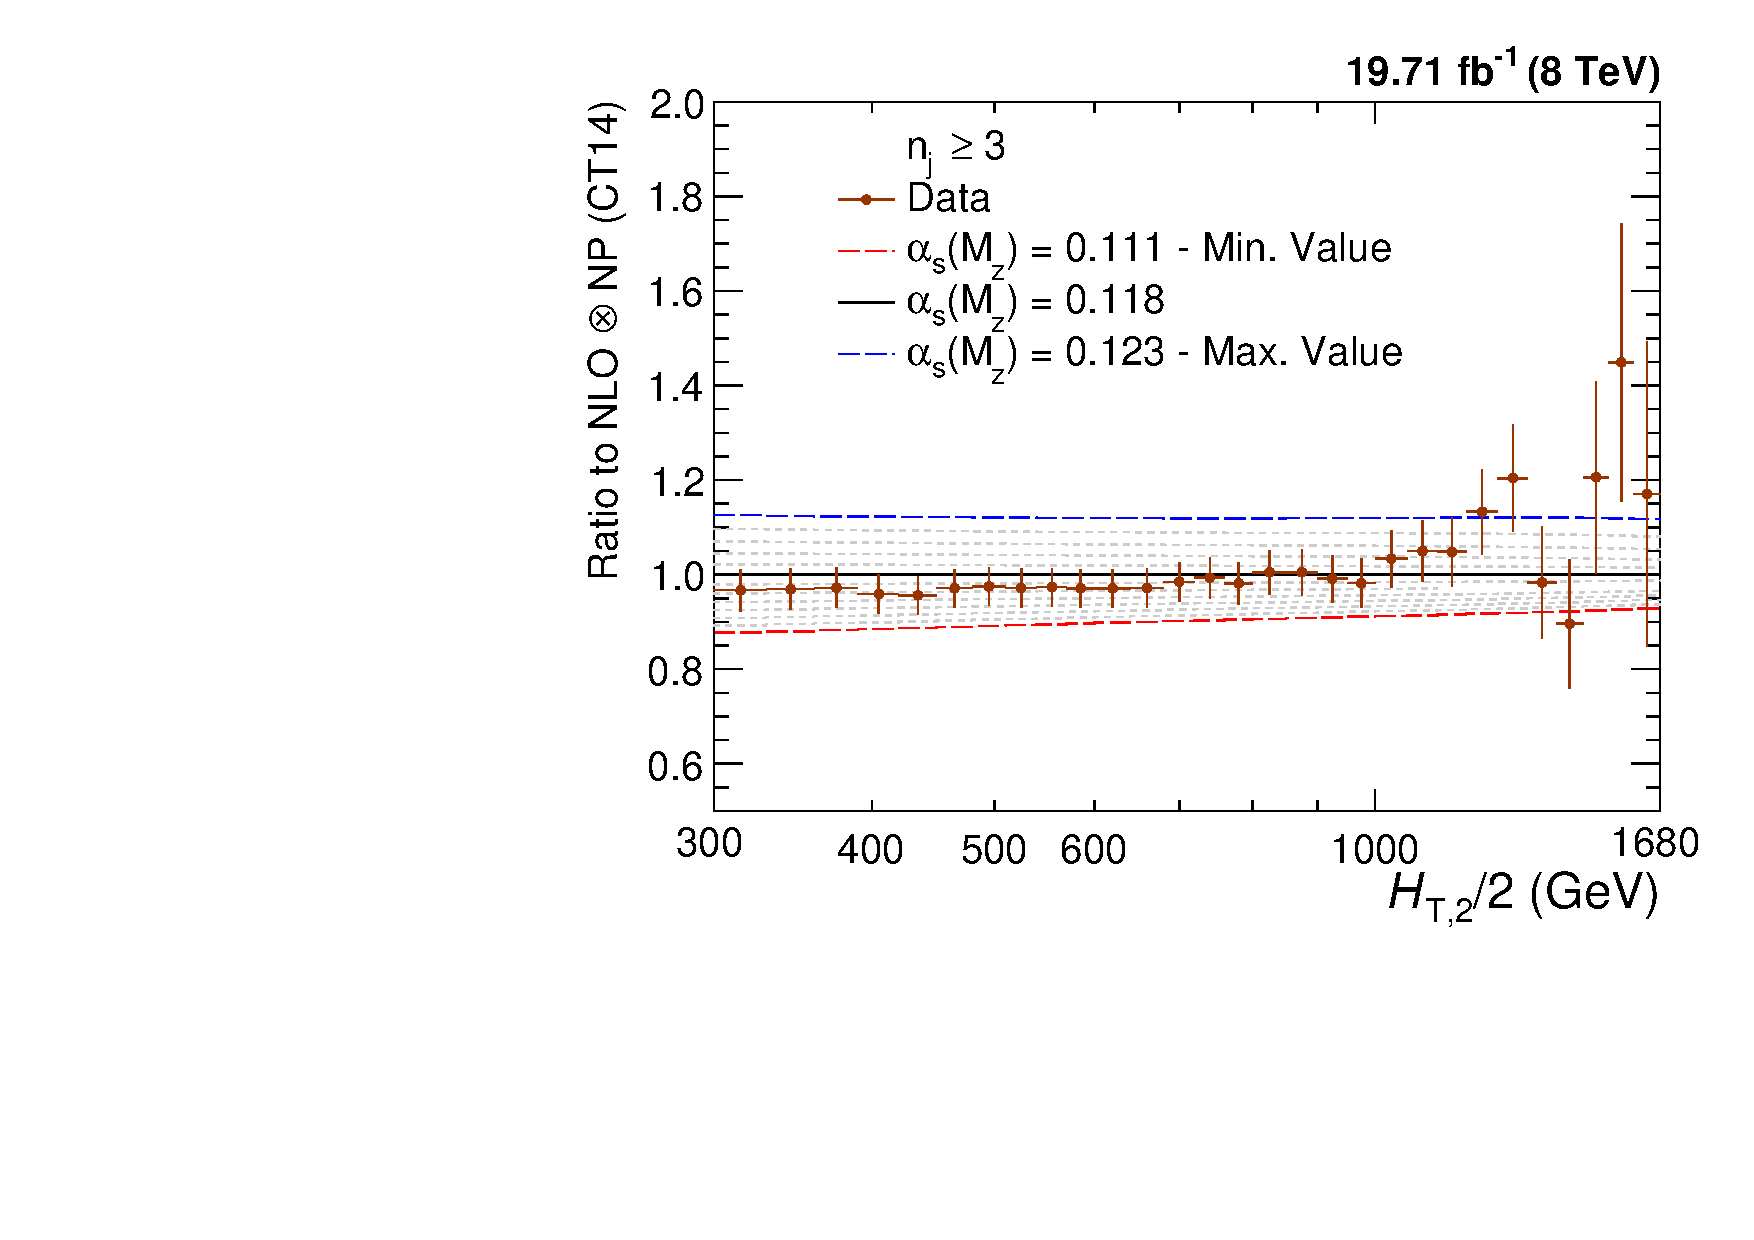
\includegraphics[scale = 0.207]{/home/anter/Desktop/Analysis_8/Present_Latex/Approval/Approval_New/Sensitivity/Sensitivity_3_ratio_NLO_CT14.pdf}%
    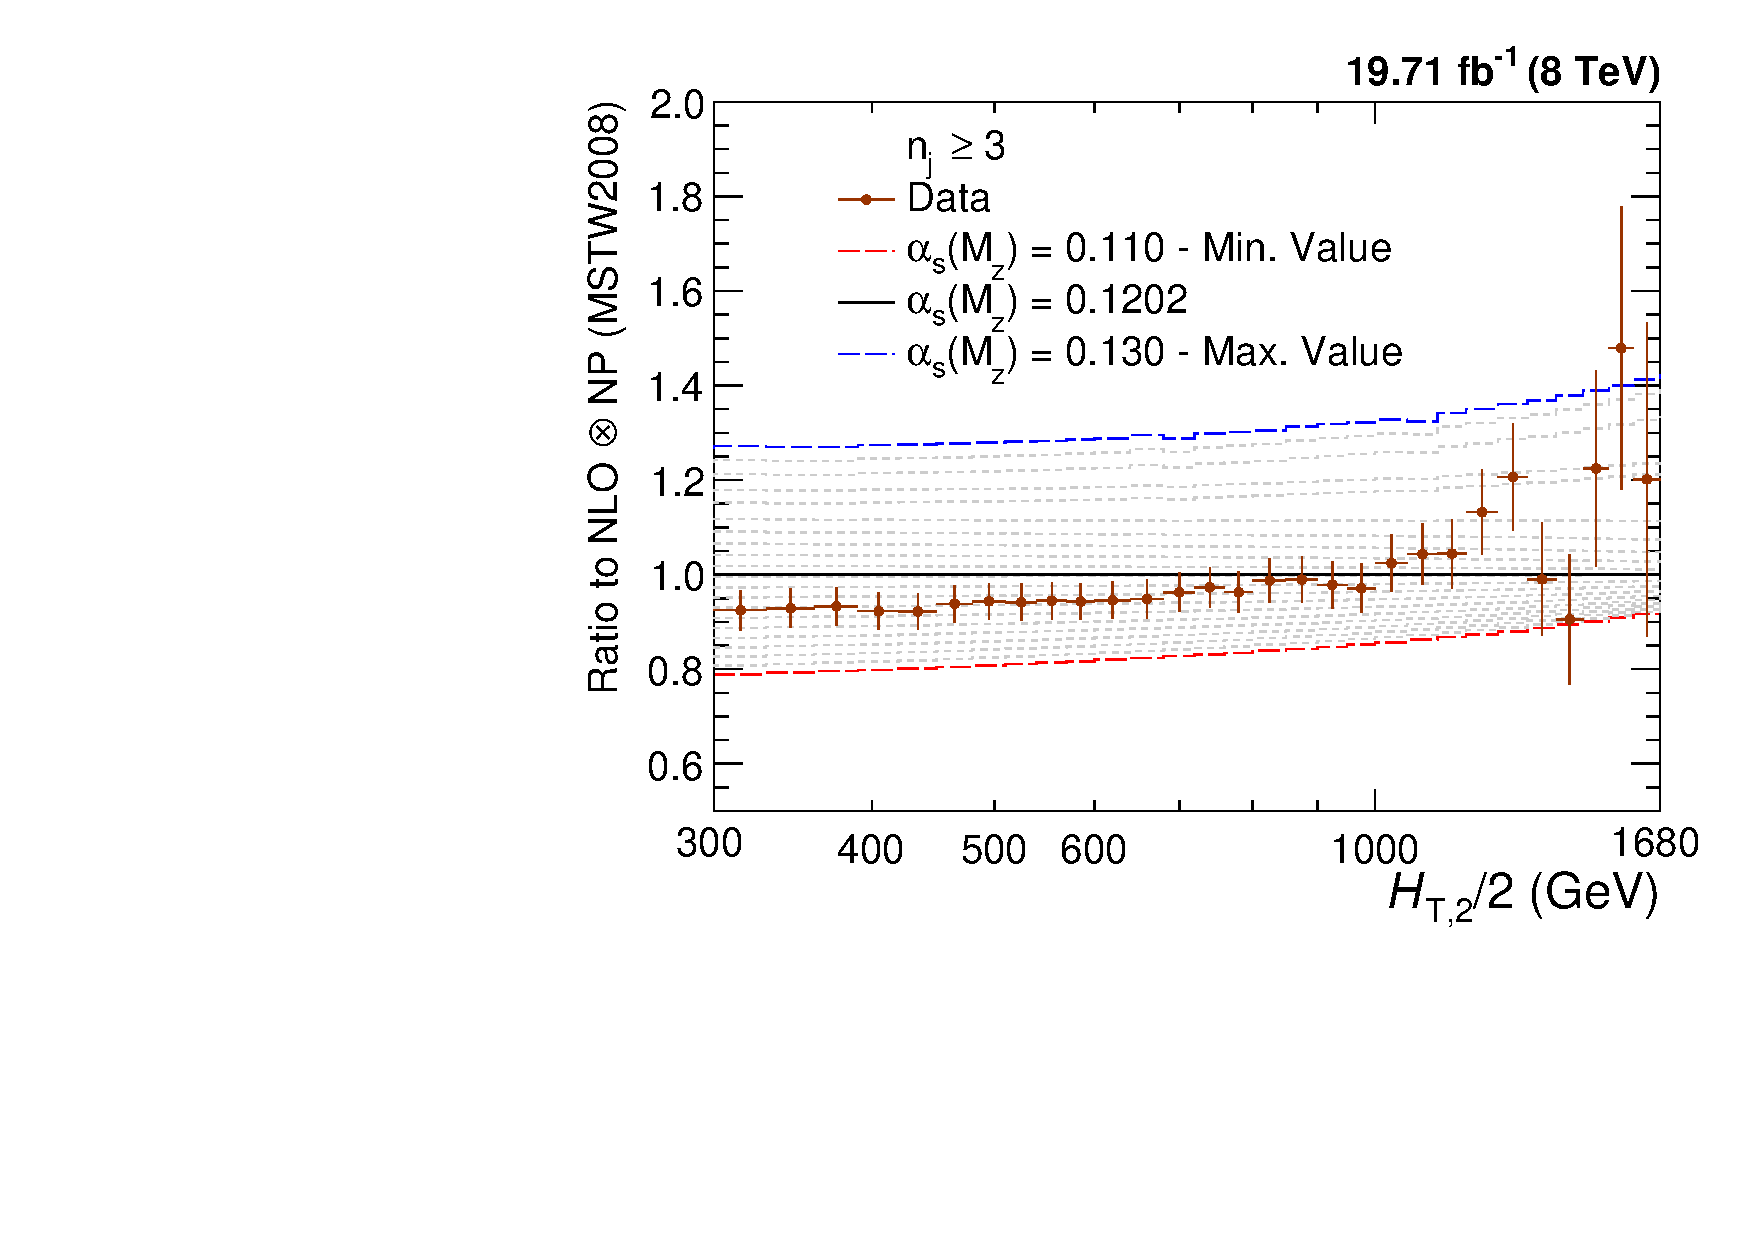
\includegraphics[scale = 0.207]{/home/anter/Desktop/Analysis_8/Present_Latex/Approval/Approval_New/Sensitivity/Sensitivity_3_ratio_NLO_MSTW2008.pdf}\\
    \vspace{5mm}
    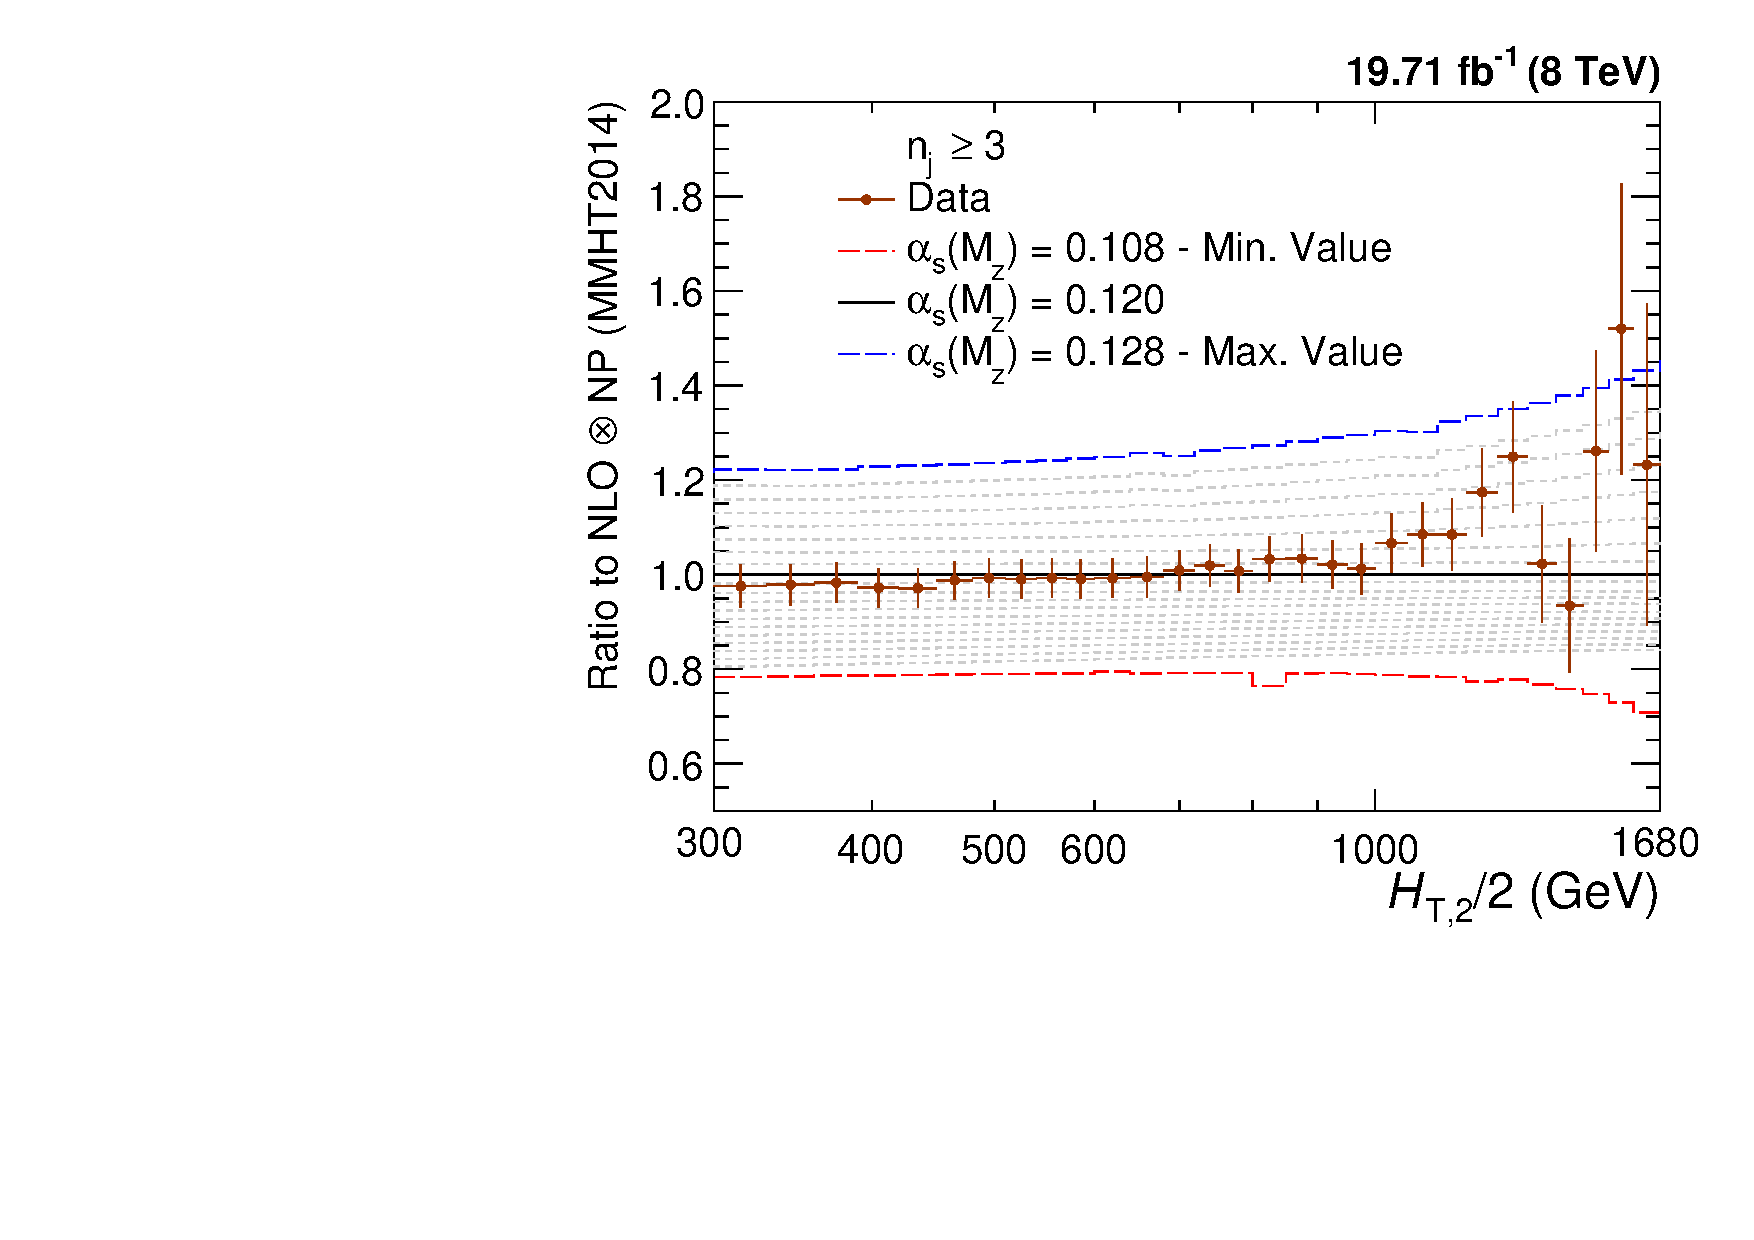
\includegraphics[scale = 0.207]{/home/anter/Desktop/Analysis_8/Present_Latex/Approval/Approval_New/Sensitivity/Sensitivity_3_ratio_NLO_MMHT2014.pdf}%
        \hspace{0.3mm}
    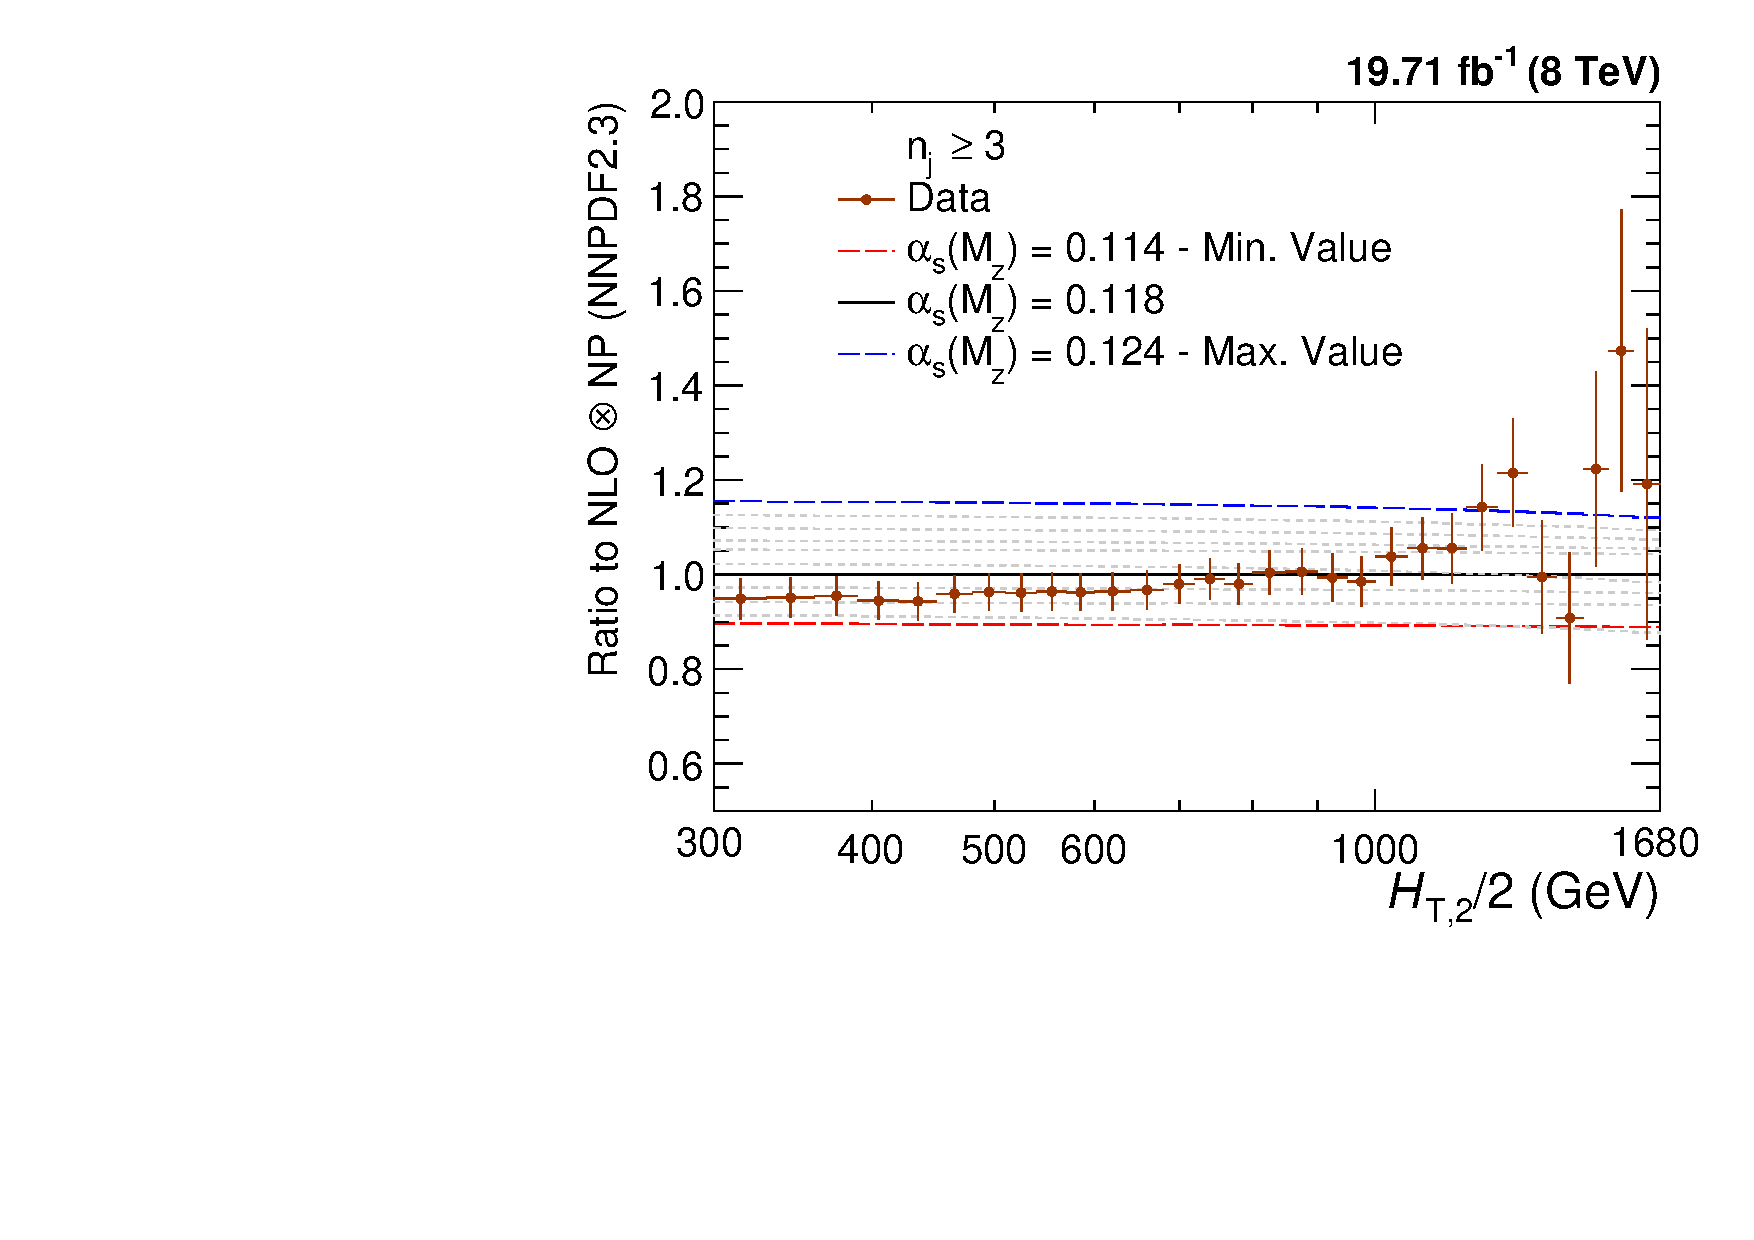
\includegraphics[scale = 0.207]{/home/anter/Desktop/Analysis_8/Present_Latex/Approval/Approval_New/Sensitivity/Sensitivity_3_ratio_NLO_NNPDF23.pdf}
\end{center}
\end{frame}

%##################################### Slide : 27 ###########################################
\begin{frame}
\frametitle{\centerline{Sensitivity of \ratio to \alpsmz}}
\setlength\labelsep   {\dimexpr\labelsep + 0.05em\relax}
\setlength\leftmargini{\dimexpr\leftmargini + 0.05em\relax}
\begin{center}
\begin{itemize}
\item {\scriptsize $\rm {\ratio \propto \alpsns^1}$ \\}
\end{itemize}
\vspace{5mm}
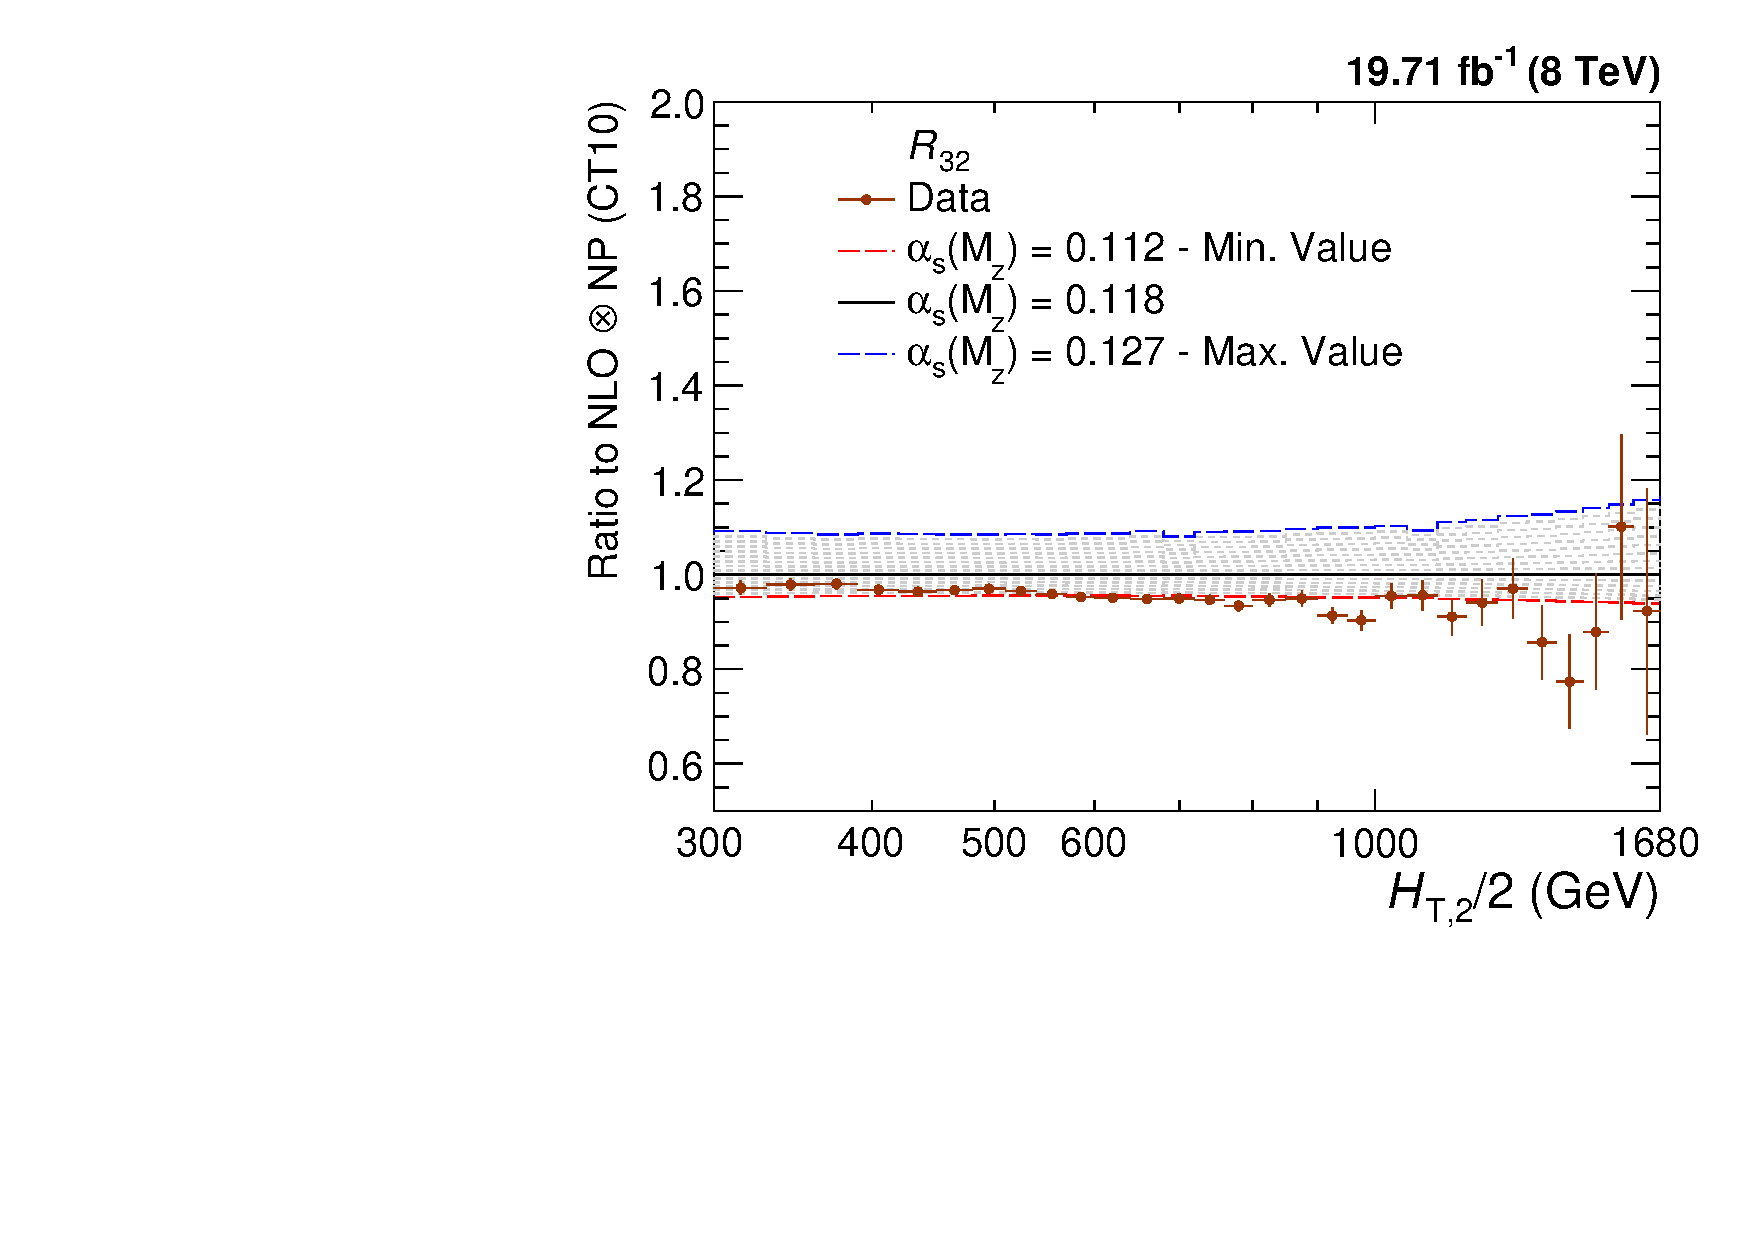
\includegraphics[scale = 0.207]{/home/anter/Desktop/Analysis_8/Present_Latex/Approval/Approval_New/Sensitivity/Sensitivity_double_ratio_32_CT10.pdf}%
    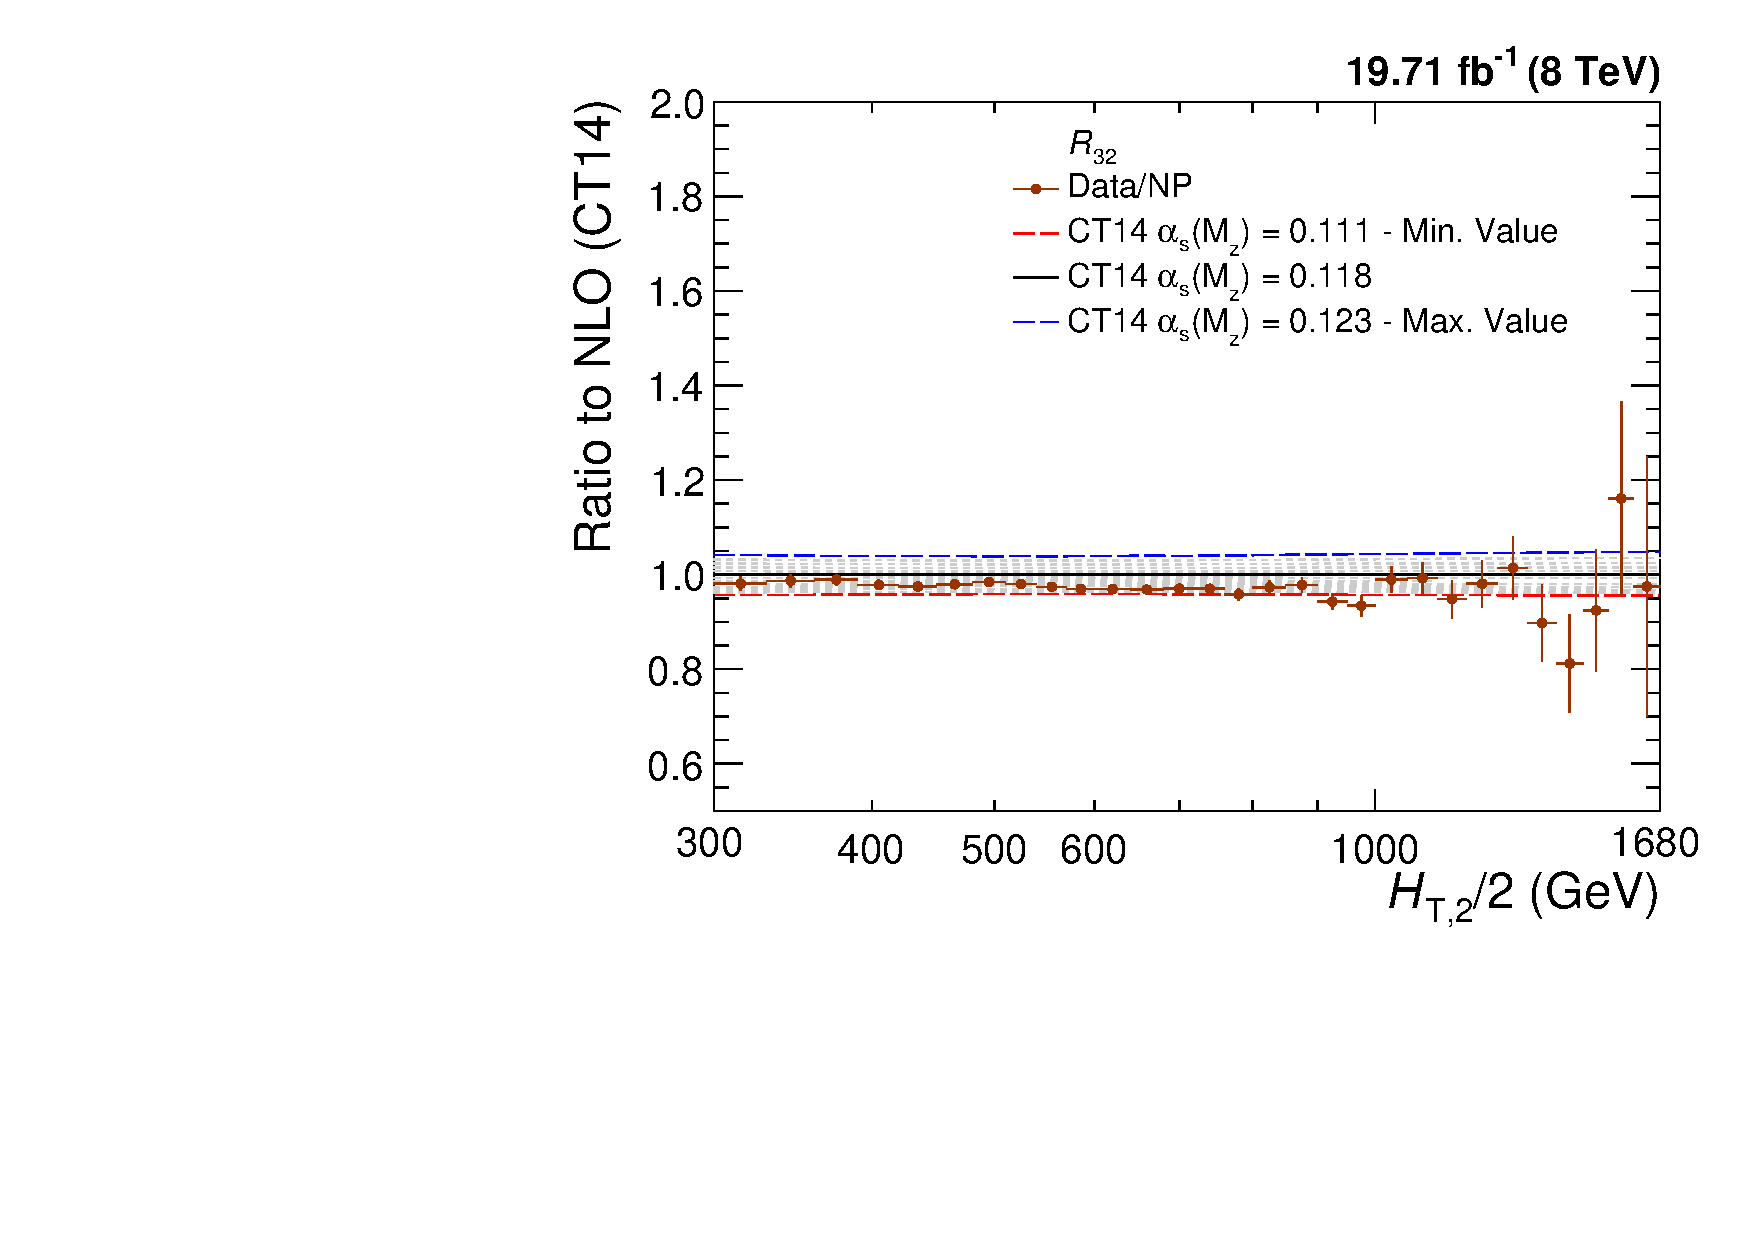
\includegraphics[scale = 0.207]{/home/anter/Desktop/Analysis_8/Present_Latex/Approval/Approval_New/Sensitivity/Sensitivity_double_ratio_32_CT14.pdf}%
    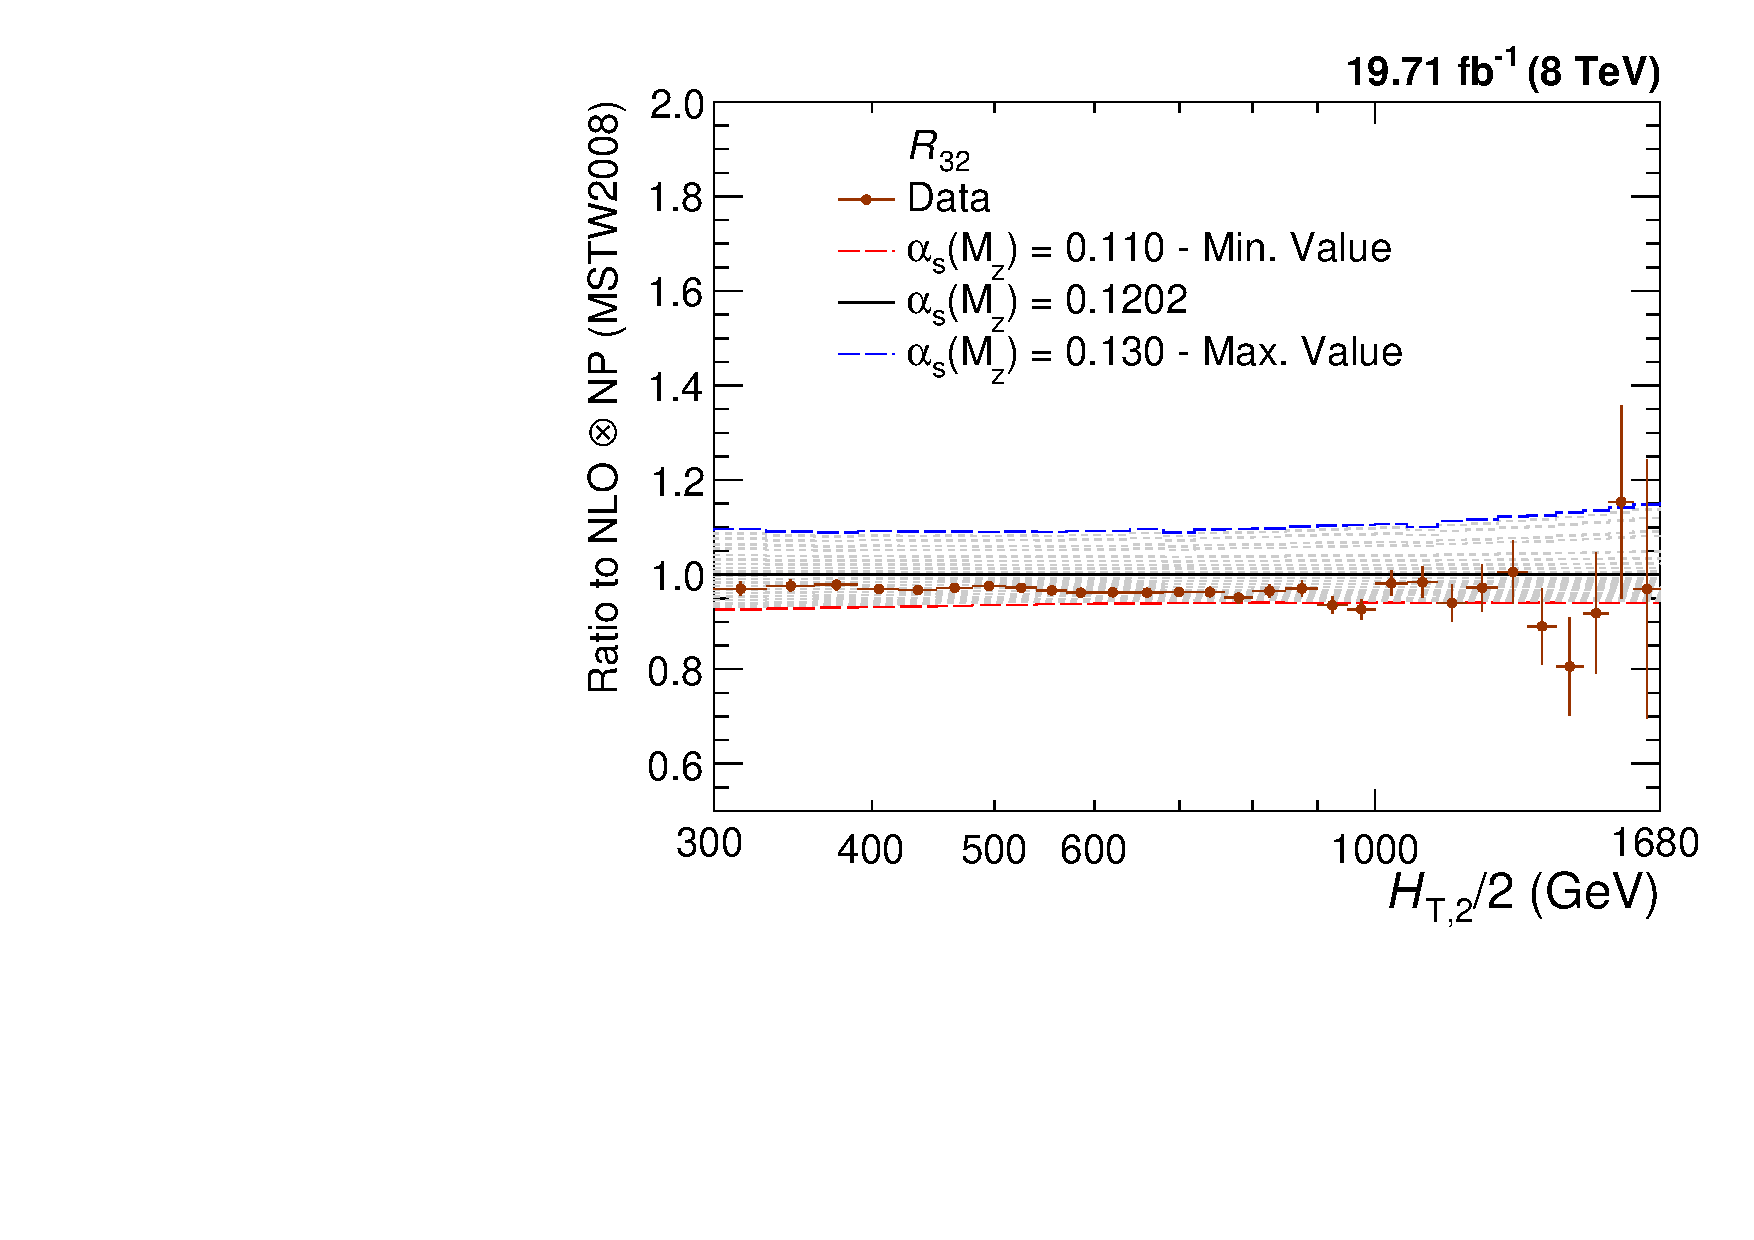
\includegraphics[scale = 0.207]{/home/anter/Desktop/Analysis_8/Present_Latex/Approval/Approval_New/Sensitivity/Sensitivity_double_ratio_32_MSTW2008.pdf}\\
      \vspace{5mm}  
    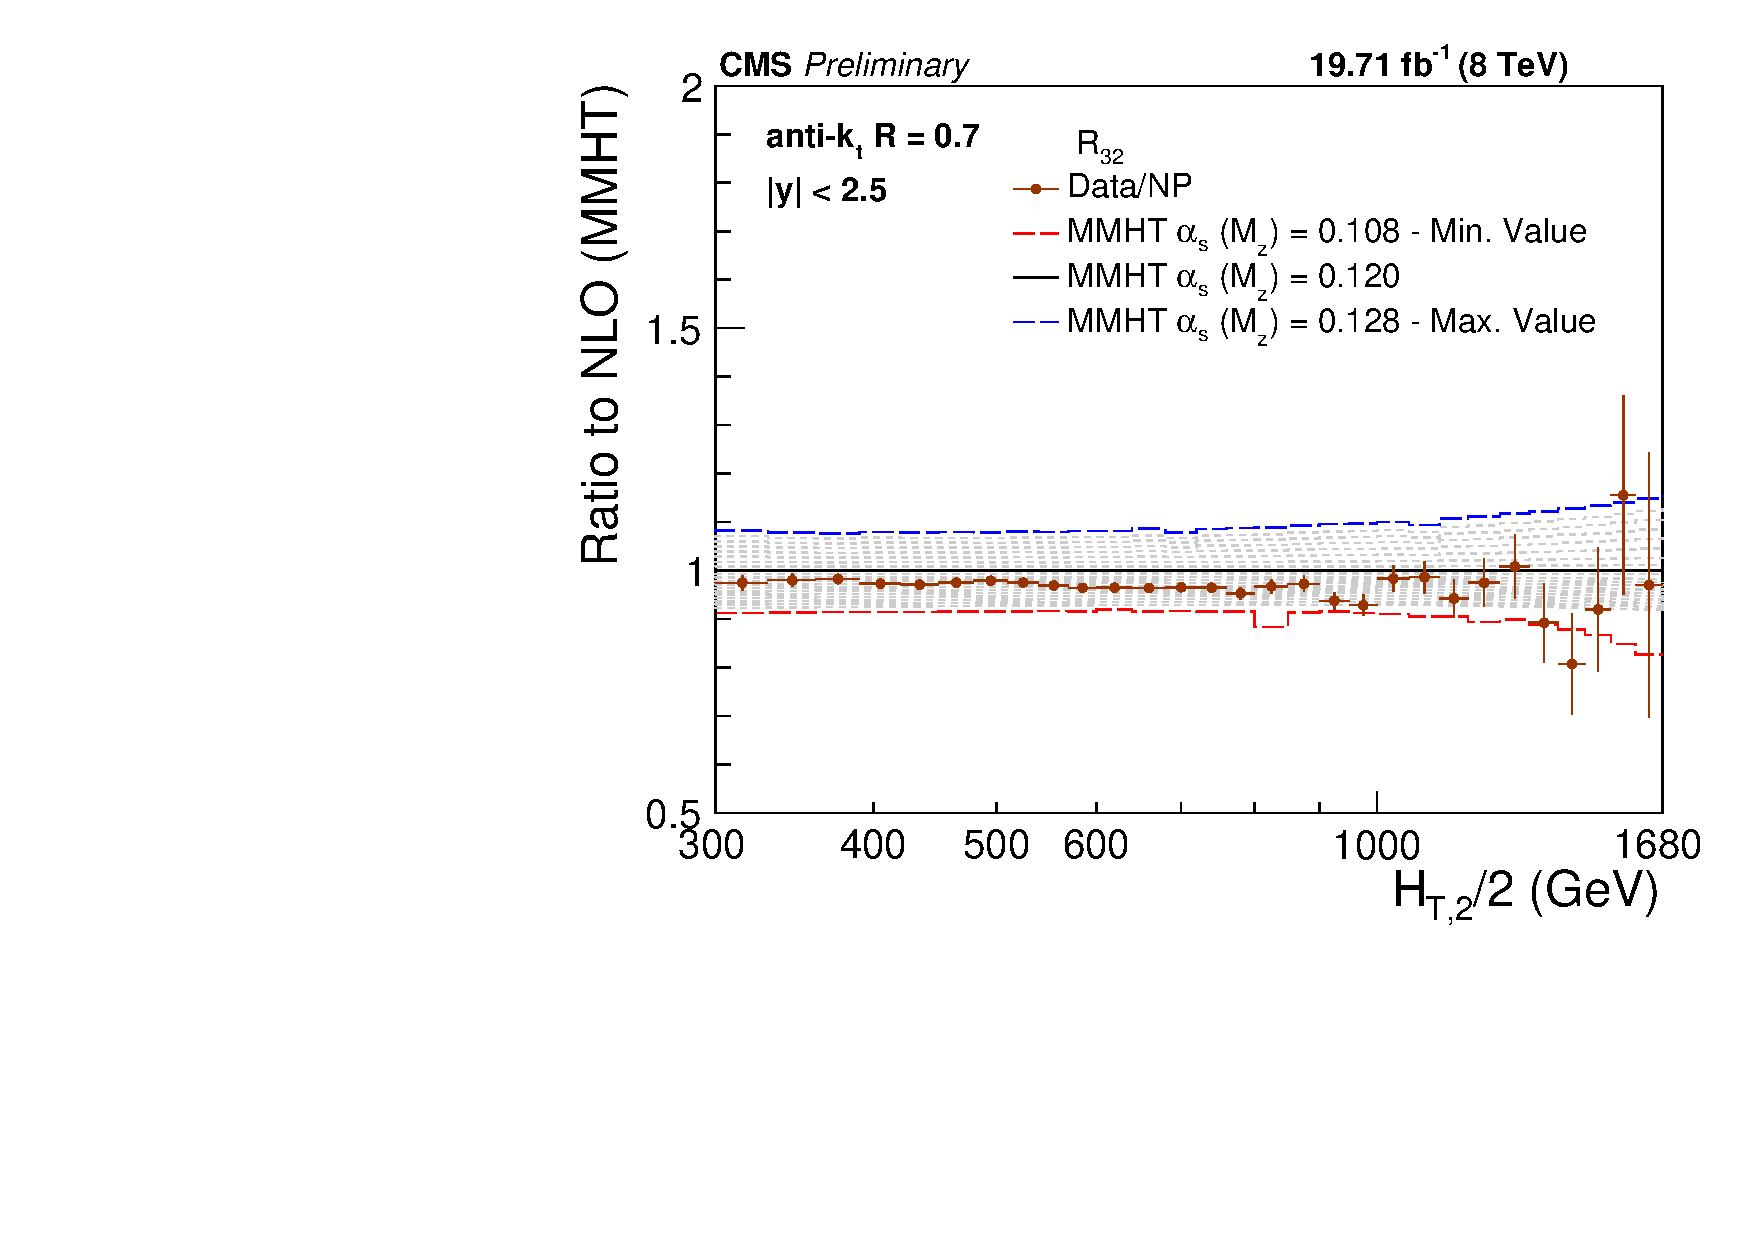
\includegraphics[scale = 0.207]{/home/anter/Desktop/Analysis_8/Present_Latex/Approval/Approval_New/Sensitivity/Sensitivity_double_ratio_32_MMHT2014.pdf}%
        \hspace{0.3mm}
    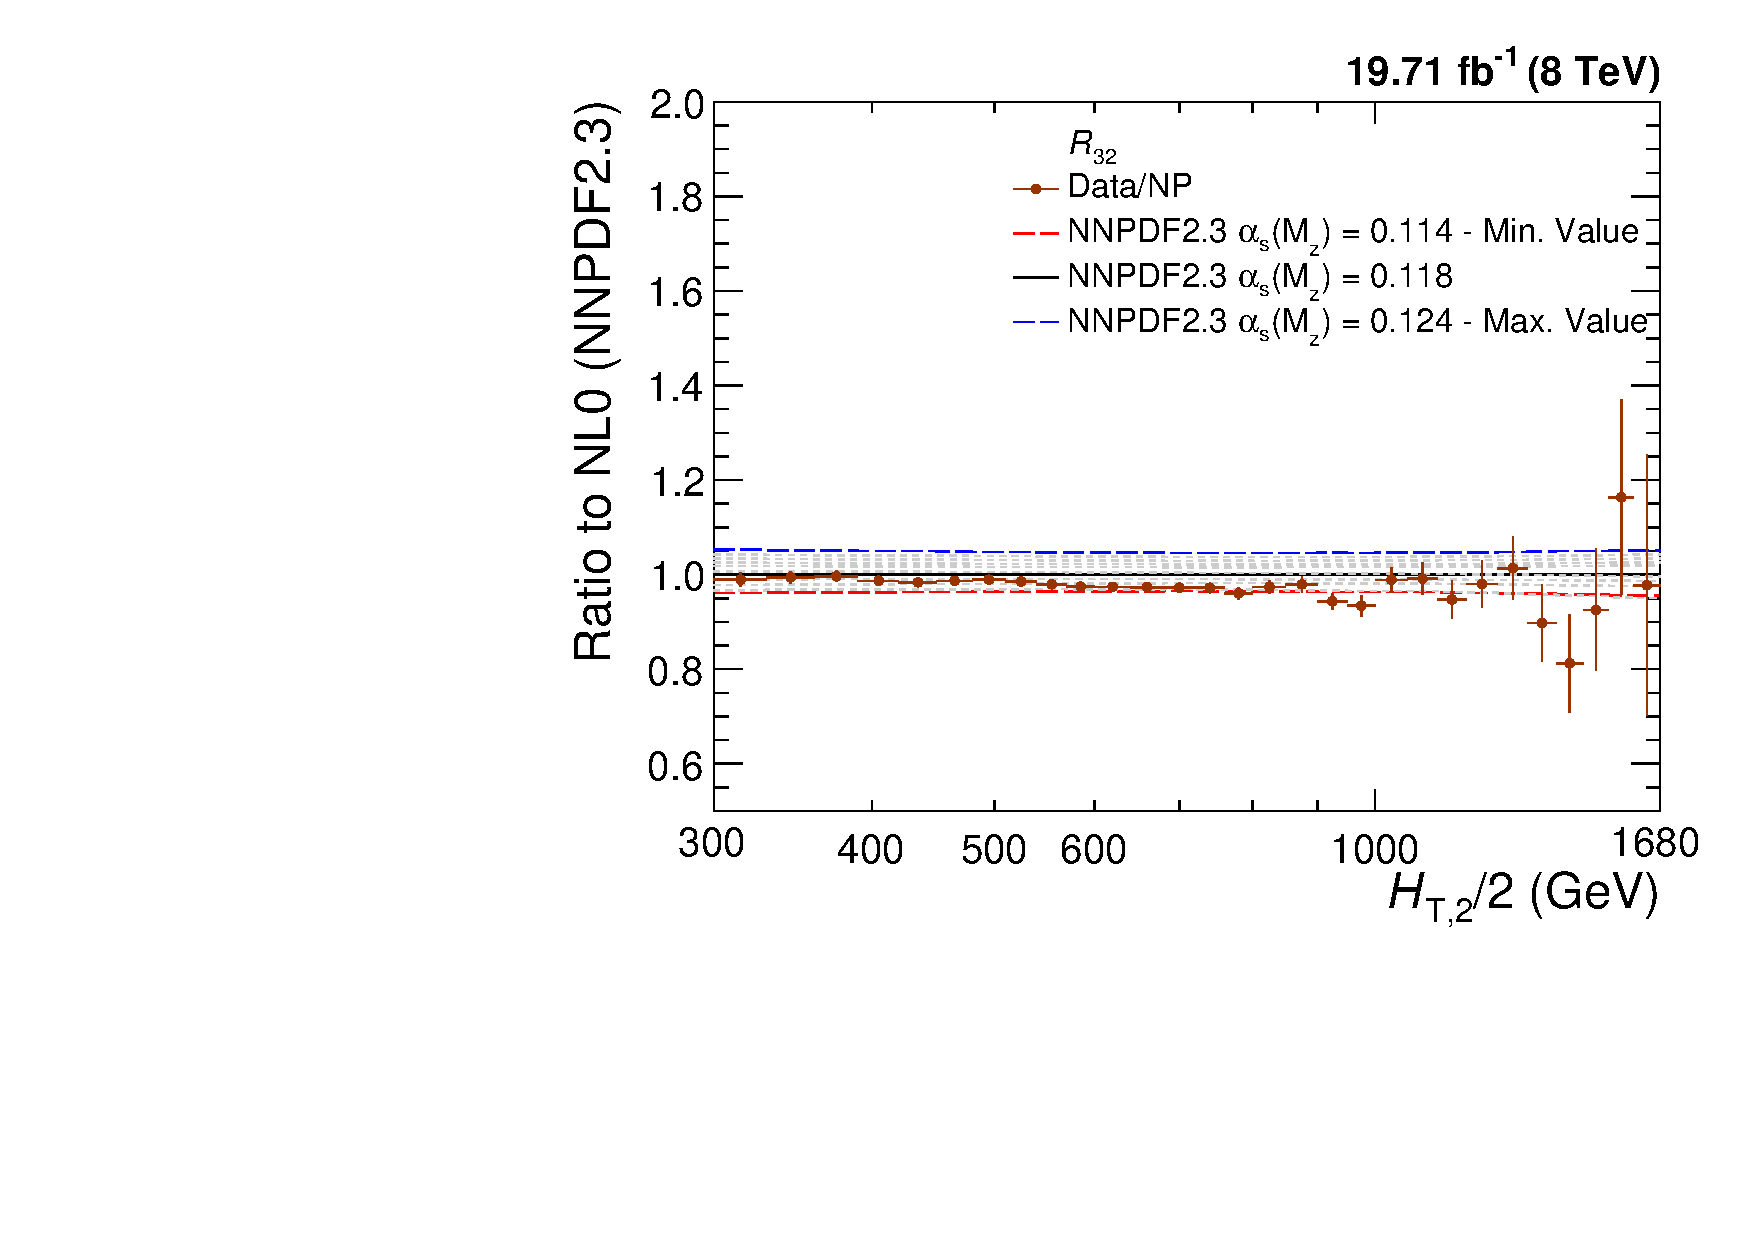
\includegraphics[scale = 0.207]{/home/anter/Desktop/Analysis_8/Present_Latex/Approval/Approval_New/Sensitivity/Sensitivity_double_ratio_32_NNPDF23.pdf}
\end{center}
\end{frame}


%##################################### Slide : 28 ###########################################
\begin{frame}
\frametitle{\centerline{Determination of the Strong Coupling Constant}}
\setlength\labelsep   {\dimexpr\labelsep + 0.05em\relax}
\setlength\leftmargini{\dimexpr\leftmargini + 0.05em\relax}
\begin{itemize}
\vspace{-2mm}
\item {\scriptsize {\bf Fit of \alps using \chsq similar to recipe as used by previous \ratio @ 7 TeV and inclusive jets @ 8 TeV analysis}\\}
\end{itemize}
\vspace{-3mm}
\begin{align*}
\resizebox{.14\hsize}{!}{$\rm \chsq = M^{T}C^{-1}M$}
\end{align*}   
\vspace{-8mm}
\begin{align*}
\resizebox{.12\hsize}{!}{$\rm M^{i}= D^{i}-T^{i}$}
\end{align*}
\vspace{-4mm}
\begin{itemize}
\item {\scriptsize $\rm{C =C_{exp} + C_{theo}}$ is defined as the sum of covariances of experimental and theoretical sources of uncertainty as follows : \\}
\end{itemize}
\begin{center}
\begin{*align} 
\resizebox{.8\hsize}{!}{$\rm  C_\mathrm{exp} = \mathrm{Cov}^\mathrm{ExpStat} ~\plus~ \sum\mathrm{Cov}^\mathrm{JEC} ~\plus~
  \mathrm{Cov}^\mathrm{Unfolding} ~\plus~
  % \mathrm{Cov}^\mathrm{JER} ~\plus~
  \mathrm{Cov}^\mathrm{Lumi} ~\plus~
  \mathrm{Cov}^\mathrm{Uncor}$}\\
  \vspace{2mm}
  \resizebox{.42\hsize}{!}{$\rm C_\mathrm{theo} = \mathrm{Cov}^\mathrm{TheoStat} ~\plus~ \mathrm{Cov}^\mathrm{NP} ~\plus~ \mathrm{Cov}^\mathrm{PDF}$}
  \end{*align}
  \end{center}
  \tri
\begin{itemize}
\begin{itemize}
\item{\tiny {$\mathrm{Cov}^\mathrm{ExpStat}$: the statistical uncertainty of the data including correlations introduced by the unfolding,}
\item{$\mathrm{Cov}^\mathrm{JEC}$: the JEC
systematic uncertainty,}
\item{$\mathrm{Cov}^\mathrm{Unfolding}$: the unfolding systematic
    uncertainty including the JER,}
\item{$\mathrm{Cov}^\mathrm{Lumi}$: the luminosity uncertainty,}
\item{$\mathrm{Cov}^\mathrm{Uncor}$: a residual uncorrelated systematic uncertainty summarizing individual causes such as trigger and identification inefficiencies, time dependence of the jet \pt resolution, and uncertainty on the trigger prescale factors,}
\item{$\mathrm{Cov}^\mathrm{TheoStat}$: the statistical uncertainty caused by numerical integrations in the cross section computations,}
\item{$\mathrm{Cov}^\mathrm{NP}$: the systematic uncertainty of the NP corrections, and}
\item{$\mathrm{Cov}^\mathrm{PDF}$: the PDF uncertainty.} \\}
\end{itemize}
\vspace{1mm}
\ball
\item {\scriptsize For the fits of the cross sections, the range in \httwo is restricted to be between 300 GeV and 1 TeV : to avoid the region close to the minimal \pt threshold of 150 GeV for each jet at low \pt and the onset of electroweak effects at high \pt\\}
\end{itemize}
\end{frame}

%##################################### Slide : 29 ###########################################
\begin{frame}
\frametitle{\centerline{Fit results in range $0.3 < \httwo < 1.00$ TeV}}
\setlength\labelsep   {\dimexpr\labelsep + 0.05em\relax}
\setlength\leftmargini{\dimexpr\leftmargini + 0.05em\relax}
\vspace{-3.4mm}
\begin{center}
\vspace{-0.4mm}
\hspace{92mm} \pas
\vspace{-2mm}
\begin{table}[htbp]
  \centering\tiny
\begin{tabular}{lcccccc}
    \hline\hline
    \multirow{2}{*}{PDF set} & \multicolumn{3}{c}{2-jets} & \multicolumn{3}{c}{3-jets} \\
    & \alpsmz & $\pm\Delta\alpsmz$ & \chisqndof &\alpsmz & $\pm\Delta\alpsmz$ & \chisqndof \\\hline
    % ABM11          & 0.1240 & 0.0025 & 11./18 & 0.1241 & 0.0020 & 10./18 \\
    CT10           & 0.1174 & 0.0032 & 3.0/18 & 0.1169 & 0.0027 & 5.4/18 \\
    CT14           & 0.1160 & 0.0035 & 3.5/18 & 0.1159 & 0.0031 & 6.1/18 \\
    MSTW2008       & 0.1159 & 0.0025 & 5.3/18 & 0.1161 & 0.0021 & 6.7/18 \\
    MMHT2014       & 0.1165 & 0.0034 & 5.9/18 & 0.1166 & 0.0025 & 7.1/18 \\
    NNPDF2.3       & 0.1183 & 0.0025 & 9.7/18 & 0.1179 & 0.0021 & 9.1/18 \\

    \hline\hline
    \end{tabular}
\end{table}
%\begin{itemize}
%\begin{itemize}
%\tri
%\item {\tiny The lower uncertainty for NNPDF2.3 suffers from a lack of smaller \alpsmz values \\}
%\end{itemize}
%\end{itemize}
\vspace{-0.5mm}
\hspace{93mm} \pas
\vspace{-5mm}
{\scriptsize {\bf \hspace {30mm} ignored correlations \hspace {10mm} accounted for correlations %in \ratio
}}\\
\vspace{-2mm}
\begin{table}[htbp]
  \centering\tiny
  \begin{tabular}{lcccccc}
    \hline\hline
    \multirow{2}{*}{PDF set} & \multicolumn{3}{c}{2- \& 3-jets} & \multicolumn{3}{c}{\ratio} \\
    & \alpsmz & $\pm\Delta\alpsmz$ & \chisqndof &\alpsmz & $\pm\Delta\alpsmz$ & \chisqndof \\\hline
    CT10           & 0.1170 & 0.0026 & 8.2/37 & 0.1141 & 0.0028 & 19./18 \rbtrr\\
    CT14           & 0.1161 & 0.0029 & 9.1/37 & 0.1139 & 0.0032 & 15./18 \rbtrr\\
    MSTW2008       & 0.1161 & 0.0021 & 11./37 & 0.1150 & 0.0023 & 21./18 \rbtrr\\
    MMHT2014       & 0.1168 & 0.0025 & 11./37 & 0.1142 & 0.0022 & 19./18 \rbtrr\\
    NNPDF2.3       & 0.1188 & 0.0019 & 15./37 & 0.1184 & 0.0021 & 12./18 \rbtrr\\
    \hline\hline
  \end{tabular}
\end{table}
\vspace{-2mm}
\begin{itemize}
%\begin{itemize}
%\tri
%\item {\scriptsize For comparison, a simultaneous fit to both cross sections ignoring any correlations, and a fit to their ratio fully accounting for correlations, is performed. \\}
%\end{itemize}
%\ball
%\vspace{2mm}
\item {\scriptsize All cross section fits give compatible values for \alpsmz in the range of 0.115~-~0.118
\vspace{1mm}
\item For \rations, smaller values are obtained as in the previous CMS \ratio publication \href{https://arxiv.org/abs/1304.7498}{[Eur. Phys. J. C 73 (2013) 2604]}
\vspace{1mm}
\item  small \chisqndof except for the \ratio fits : may be due to an overestimation of the residual uncorrelated uncertainty of 1\% that is cancelled for \ratio . 
\vspace{1mm}
\item With an assumed uncertainty of 0.25\% : the \chisqndof values lie around unity while the \alpsmz values are still compatible with the previous results but with slightly reduced uncertainties. \\}
\end{itemize}
\end{center}
\end{frame}

%##################################### Slide : 30 ###########################################
\begin{frame}
\frametitle{\centerline{Fit results in range $0.3 < \httwo < 1.68$ TeV}}
\setlength\labelsep   {\dimexpr\labelsep + 0.05em\relax}
\setlength\leftmargini{\dimexpr\leftmargini + 0.05em\relax}
\begin{center}
\vspace{-3mm}
\begin{itemize}
\item {\scriptsize \alpsmz fits to the 2-jet event cross section with or without EWK correction factors. \\}
\tri 
\begin{itemize}
\item {\scriptsize Reduction in \chisqndof indicating a better agreement when EWK effects are included. 
\vspace{1mm}
\item A tendency to slightly smaller \alpsmz values is observed without the EWK corrections. \\}
\end{itemize}
\ball
\end{itemize}
\vspace{-2mm}
\hspace{93mm} \pas
\vspace{-2mm}
\begin{table}[p]
   \centering\tiny
  \begin{tabular}{lcccccc}
    \hline\hline
    \multirow{2}{*}{PDF set} & \multicolumn{3}{c}{2-jets, without EWK} &
    \multicolumn{3}{c}{2-jets, with EWK} \\
    & \alpsmz & $\pm\Delta\alpsmz$ & \chisqndof &\alpsmz & $\pm\Delta\alpsmz$ & \chisqndof \\\hline
    CT10           & 0.1163 & 0.0034 & 15./28 & 0.1165 & 0.0032 & 14./28 \rbtrr\\
    CT14           & 0.1137 & 0.0033 & 24./28 & 0.1144 & 0.0033 & 17./28 \rbtrr\\
    MSTW2008       & 0.1093 & 0.0028 & 27./28 & 0.1133 & 0.0023 & 19./28 \rbtrr\\
    MMHT2014       & 0.1127 & 0.0032 & 32./28 & 0.1141 & 0.0032 & 21./28 \rbtrr\\
    NNPDF2.3       & 0.1162 & 0.0024 & 31./28 & 0.1168 & 0.0024 & 23./28 \rbtrr\\
    \hline\hline
  \end{tabular}
\end{table}

\begin{itemize}
\item {\scriptsize Results from the two most compatible PDF sets MSTW2008 and MMHT2014 at NLO : \\}
\tri 
\begin{itemize}
\item {\scriptsize provide a large enough range in \alpsmz values to ensure fits without extrapolation
\vspace{1mm}
\item Other three PDF sets are at the limit such that reliable fits cannot be performed for estimation of all uncertainties. \\}
\end{itemize}
\ball 
\end{itemize}
\vspace{-2mm}
\hspace{83mm} \pas
\vspace{-2mm}
\begin{table}[p]
   \centering\tiny
  \begin{tabular}{lccccccc}
    \hline\hline
    \multirow{2}{*}{PDF set} & & \multicolumn{5}{c}{\ratio: $\Delta\alpsmz\times1000$} & \\
    & \alpsmz & exp & PDF & NP & all exc.\ scale & scale & \chisqndof \\\hline
    MSTW2008       & 0.1150 & $\pm10$ & $\pm13$ & $\pm15$ & $\pm23$ & $^{+50}_{-0}$ & 26./28 \\
    MMHT2014       & 0.1142 & $\pm10$ & $\pm13$ & $\pm14$ & $\pm22$ & $^{+49}_{-6}$ & 24./28 \\
    \hline\hline
  \end{tabular}
\end{table}
\end{center}
\end{frame}

%##################################### Slide : 31 ###########################################
\begin{frame}
\frametitle{\centerline{Fit results in range $0.3 < \httwo < 1.68$ TeV}}
\setlength\labelsep   {\dimexpr\labelsep + 0.05em\relax}
\setlength\leftmargini{\dimexpr\leftmargini + 0.05em\relax}
\begin{center}
\vspace{-1mm}
%
% Scale variations
%
\vspace{-2mm}
\begin{itemize}
\item {\scriptsize Using \ratio at the central scale and for the six scale factor combinations for the two PDF sets MSTW2008 and MMHT2014\\}
\end{itemize}
\hspace{78mm} \pas
\vspace{-2mm}
\begin{table}[htbp]
  \centering\tiny
  \begin{tabular}{cccccc}
    \hline\hline
    \multirow{2}{*}{$\mur/\httwo$} & \multirow{2}{*}{$\muf/\httwo$} &
    \multicolumn{2}{c}{MSTW2008} & \multicolumn{2}{c}{MMHT2014}\rbtrr\\
    & & \alpsmz & \chisqndof & \alpsmz & \chisqndof\rbthm\\\hline

    $1$    & $1$    & $0.1150$ & $26./28$ & $0.1142$ & $24./28$ \\
    $1/2$  & $1/2$  & $0.1165$ & $77./28$ & $0.1160$ & $73./28$ \\
    $2$    & $2$    & $0.1120$ & $18./28$ & $0.1191$ & $18./28$ \\
    $1/2$  & $1$    & $0.1150$ & $53./28$ & $0.1136$ & $48./28$ \\
    $1$    & $1/2$  & $0.1150$ & $30./28$ & $0.1142$ & $28./28$ \\
    $1$    & $2$    & $0.1155$ & $23./28$ & $0.1147$ & $22./28$ \\
    $2$    & $1$    & $0.1180$ & $19./28$ & $0.1175$ & $19./28$ \\
    \hline\hline
  \end{tabular}
\end{table}
%
% Q bins
%
\vspace{-2mm}
\begin{itemize}
\item {\scriptsize Uncertainty composition for \alpsmz from the determination of \alps in bins of \httwo \\}
\end{itemize}
\hspace{100mm} \pas
\vspace{-2mm}
\begin{table}[htbp]
  \centering\tiny
  \begin{tabular}{ccccccccccc}
    \hline\hline
    \httwo & % $\langle{}Q\rangle$ &
    \multicolumn{5}{c}{MSTW2008: $\Delta\alpsmz\times1000$} &
    \multicolumn{5}{c}{MMHT2014: $\Delta\alpsmz\times1000$} \\
    (GeV) & % (\GeV) &
    \alpsmz & exp & PDF & NP & scale &
    \alpsmz & exp & PDF & NP & scale \\ \hline
    300--420   & 0.1157 & $\pm{15}$ & $\pm{14}$    & $\pm{19}$     & $^{+53}_{-0}$ &
    0.1158 & $\pm{14}$ & $\pm{10}$    & $\pm{19}$     & $^{+52}_{-0}$\\
    420--600 & 0.1153 & $\pm{11}$ & $\pm{14}$    & $\pm{18}$     & $^{+57}_{-0}$ &
    0.1154 & $\pm{11}$ & $\pm{12}$    & $\pm{17}$     & $^{+56}_{-0}$\\
    600--1000 & 0.1134 & $\pm{13}$ & $\pm{16}$    & $\pm{19}$     & $^{+52}_{-0}$ &
    0.1140 & $\pm{12}$ & $\pm{12}$    & $\pm{18}$     & $^{+45}_{-0}$\\
    1000--1680 & 0.1147 & $\pm{29}$ & $\pm{17}$    & $\pm{18}$     & $^{+63}_{-11}$ &
    0.1154 & $\pm{25}$ & $\pm{14}$    & $\pm{15}$     & $^{+56}_{-11}$\\\hline
    300--1680 & 0.1150 & $\pm{10}$ & $\pm{13}$    & $\pm{15}$     & $^{+50}_{-0}$ &
    0.1142 & $\pm{10}$ & $\pm{13}$    & $\pm{14}$     & $^{+49}_{-6}$\\
    \hline\hline
  \end{tabular}
\end{table}
\end{center}
\end{frame}

%##################################### Slide : 32 ###########################################
\begin{frame}
\frametitle{\centerline{Summary}}
\setlength\labelsep   {\dimexpr\labelsep + 0.05em\relax}
\setlength\leftmarginiii{\dimexpr\leftmarginiii + 0.05em\relax}
\vspace{-3.5mm}
\begin{center}
\begin{itemize}
\item {\scriptsize A measurement of the inclusive 2-jet (3-jet) event cross sections has been presented in a range of $0.3 < \httwo < 2.0$ TeV ($0.3 < \httwo < 1.68$ TeV) for the average \pt of the two leading jets at central rapidity of $|$y$|$ $<$ 2.5
\vspace{0.5mm}
\item Measured cross sections are corrected for detector effects and compared to NLO calculations
\vspace{0.5mm}
\item Compared to the different PDF sets \\}
\vspace{0.5mm}
\tri
\begin{itemize}
\item {\tiny Well described by calculations at NLO in pQCD complemented with NP corrections that are important at low \httwo \\}
\end{itemize}
\ball
\vspace{0.5mm}
\item {\scriptsize Compared to the different Monte Carlo generators \\}
\vspace{0.5mm}
\tri
\begin{itemize}
\item {\tiny LO tree-level MC predictions exhibit significant deviations. \\}
\end{itemize}
\ball
\vspace{0.5mm}
\item {\scriptsize \alpsmz Determination \\}
\vspace{0.5mm} 
\tri
\begin{itemize}
\item {\tiny Performed fits of \alpsmz from differential inclusive 2-jet and inclusive 3-jet event cross-sections separately and in combined fit as well as ratio \ratio, in the range in \httwo of 0.3 TeV up to 1.00 TeV.
\vspace{0.5mm}
\item MSTW2008 and MMHT2014 PDF sets provide a large enough range in \alpsmz values and give similar results in full range in \httwo of 0.3 TeV up to 1.68 TeV and for scale variations in this range, and also for subranges in \httwo 
\vspace{0.5mm}
\item Using MSTW2008 PDF set, the strong coupling constant is determined in a fit to the \ratio measurement to : \\}
\end{itemize}
\end{itemize}
\ball
%\vspace{-5mm}
\vspace{-2mm}
\begin{align*}
 \resizebox{.78\hsize}{!}{$\rm {\bf {\green {\alpsmz = 0.1150\,\pm0.0010\,\textrm{(exp)}\,\pm0.0013\,\textrm{(PDF)}\,\pm0.0015\,\textrm{(NP)}\,^{+0.0050}_{-0.0000}\,\textrm{(scale)}}}}$}
  \end{align*}
\vspace{-8mm}
  \begin{align*}
  \resizebox{.6\hsize}{!}{$\rm {\bf {\green {= 0.1150\,\pm0.0023\,\textrm{(all except scale)}\,^{+0.0050}_{-0.0000}\,\textrm{(scale)}\ ~~~~~~~~~~~~~~~~ \! \! \! }}}$}
\end{align*}
\vspace{-5mm}
\begin{itemize}
\tri
\begin{itemize}
\item {\tiny Agreement with the world average value of a {\bf \alpsmz = 0.1181 $\pm$ 0.0011 }\\}
\end{itemize}
\end{itemize}
\end{center}
{\normalsize{\bf We kindly request for the approval of this analysis. Thank you !!} \\}
\end{frame}
 \ball
 
 %##################################### Slide : 33 ###########################################
\begin{frame}
\begin{center}
\vspace{15mm}
\textbf{\Large\mycolor{Back-Up Slides}}
\end{center}
\end{frame}

%##################################### Slide : 35 ###########################################
\begin{frame}
\frametitle{\centerline{Previous Results}}
\setlength\labelsep   {\dimexpr\labelsep + 0.05em\relax}
\setlength\leftmargini{\dimexpr\leftmargini + 0.05em\relax}
\vspace{-0.5mm}
\begin{minipage}[thbp]{0.3\textwidth} 
\includegraphics[scale=0.20]{/home/anter/Desktop/Analysis_8/Present_Latex/Pre-approval/Pre_results/NNPDF_R32_150_as_AK7.pdf}\\
\vspace{-0.5mm}
\includegraphics[scale=0.30]{/home/anter/Desktop/Analysis_8/Present_Latex/Approval/Approval/8TeV.pdf}
\end{minipage}
\hspace{20mm}
\begin{minipage}[thbp]{0.48\textwidth} 
\begin{itemize}
\item {\scriptsize Ratio of inclusive 3\mbox{-} to 2\mbox{-}jet events = $\frac{\sigma_{3\mbox{-}jet}}{\sigma_{2\mbox{-}jet}}$ $\propto$ \alps vs \ptave at $\sqrt{s}$ = 7 TeV
\item Comparison with NLO calculations
\item \alpsmz = 0.1148 $\pm$ 0.0014 (exp.) $\pm$ 0.0018 (PDF) $\pm$ 0.0050 (theory) ~~~~~~~~= {\bf 0.1148 $\pm$ 0.0055}
\item \blue {{\bf 7 TeV Published}} 
\item {\bf Eur. Phys. J. C 73 (2013) 2604} 
\vspace{10mm}
\item Measurement and QCD analysis of double-differential inclusive jet cross-sections in pp collisions at sqrt(s) = 8 TeV and ratios to 2.76 and 7 TeV 
\item \alpsmz (NLO) = 0.1164$^{\plus0.0025}_{\text{-}0.0029}$(PDF) $^{\plus0.0053}_{\text{-}0.0028}$(Scale)$\pm$ 0.0001(NP)$^{\plus0.0014}_{\text{-}0.0015}$(Exp) = {\bf 0.1164$^{\plus{\bf 0.0060}}_{\text{-}{\bf 0.0043}}$}
\item \mycolor {{\bf 8 TeV Submitted}}
\item {\bf arXiv:1609.05331 }\\ }
\end{itemize}
\end{minipage}
\end{frame}

%##################################### Slide : 4 ###########################################
\begin{frame}
\frametitle{\centerline{Introduction}}
\setlength\labelsep   {\dimexpr\labelsep + 0.05em\relax}
\setlength\leftmargini{\dimexpr\leftmargini + 0.05em\relax}
\begin{center}
\vspace{-4.0mm}
\begin{itemize}
\item {\scriptsize The measurement of inclusive multijet event cross-sections, \\}
\end{itemize}
\vspace{-7.0mm}
\begin{align*}
\hspace{30mm}\resizebox{.55\hsize}{!}{$\rm \sigma_{i\mbox{-}jet} = \sigma(pp\to i~jets~\plus~X) \propto \alpsns^{i}$ ~~~~~~~~{\mycolor {\bf$^{*}$to be fixed in text}}} 
\end{align*}
\vspace{-7.0mm}
\tri
\begin{itemize}
\begin{itemize}
\item {\scriptsize and their ratio \\ }
\end{itemize}
\end{itemize}
\vspace{-4.0mm}
\begin{align*}
\resizebox{.3\hsize}{!}{$\rm{R_{mn} = \frac{\sigma_{m\mbox{-}jet}}{\sigma_{n\mbox{-}jet}}} \propto \alpsns^{m-n}~;~ m~>~n$} \\ 
\end{align*}
\vspace{-10.0mm}
\begin{itemize}
\tri
\begin{itemize}
\item {\scriptsize as a function of \\}
\end{itemize}
\end{itemize}
\vspace{-7.0mm}
\begin{align*}
 \resizebox{.3\hsize}{!}{$\ptave = \mathrm{\frac{p_{T,1} + p_{T,2}}{2}} = \httwo $}
\end{align*}
\vspace{-6.0mm}
\ball
\begin{itemize}
\item {\scriptsize The inclusive differential multijet event cross section is defined as : \\}
\vspace{-6mm}

\begin{align*}
\resizebox{.45\hsize}{!}{$\mathrm{\frac{d\sigma}{d(H_{T,2}/2)}} =  \frac{1}{\epsilon~\mathcal{L}_{\mathrm{int,eff}}}\frac{N_\mathrm{event}}{\Delta\big(\httwo\big)}, ~\mathrm{where}$}
\end{align*}
\cir
\begin{itemize}
\begin{itemize}
\vspace{-4mm}
{\scriptsize \item $\epsilon$ : the product of the trigger and jet selection efficiencies and $>$ 99\%,
\item $\mathcal{L}_{\mathrm{int,eff}}$ : the effective integrated luminosity,
\item $\it{N}_\mathrm{event}$ : the number of 2- or 3-jet events counted in an \httwo bin, and
\item $\Delta\big(\httwo\big)$ : the bin widths. The measurements are reported in units of (pb/GeV). \\}
\end{itemize}
\end{itemize}
\vspace{0.5mm}
\ball
\item {\scriptsize The measured cross-section is corrected for detector effects and is  compared to the ~~~~NLO $\otimes$ NP QCD predictions for different PDF sets
\vspace{1.0mm}
\item Fits of the strong coupling constant are performed for inclusive 2\mbox{-}jet and 3\mbox{-}jet event cross-sections separately and for their ratio \ratio 
\vspace{1.0mm}
\item In the talk : \\}
\tri
\begin{itemize}
\item {\scriptsize Highlighted text in \green{green} $\rightarrow$ {\bf changed during ARC review}
\vspace{1.0mm}
\item Inclusive 2\mbox{-}jet : {\bf $\rm{n_{ j} \geq }$~2} \green{(300--2000 GeV)}, Inclusive 3\mbox{-}jet : {\bf $\rm{n_{ j} \geq }$~3} \green{(300--1680 GeV)}, Inclusive 4\mbox{-}jet : {\bf $\rm{n_{ j} \geq }$~4} \mycolor{(only in AN for now)} and ratio : \ratio \green{(300--1680 GeV)} \\}
\end{itemize}
\end{itemize}
\end{center}
\end{frame}
\ball
%##################################### Slide : 36 ###########################################
\begin{frame}
\frametitle{\centerline{Trigger Efficiencies vs \httwo}}
\setlength\labelsep   {\dimexpr\labelsep + 1.0em\relax}
\setlength\leftmargini{\dimexpr\leftmargini + 1.0em\relax}
\vspace{-3mm}
\begin{center}
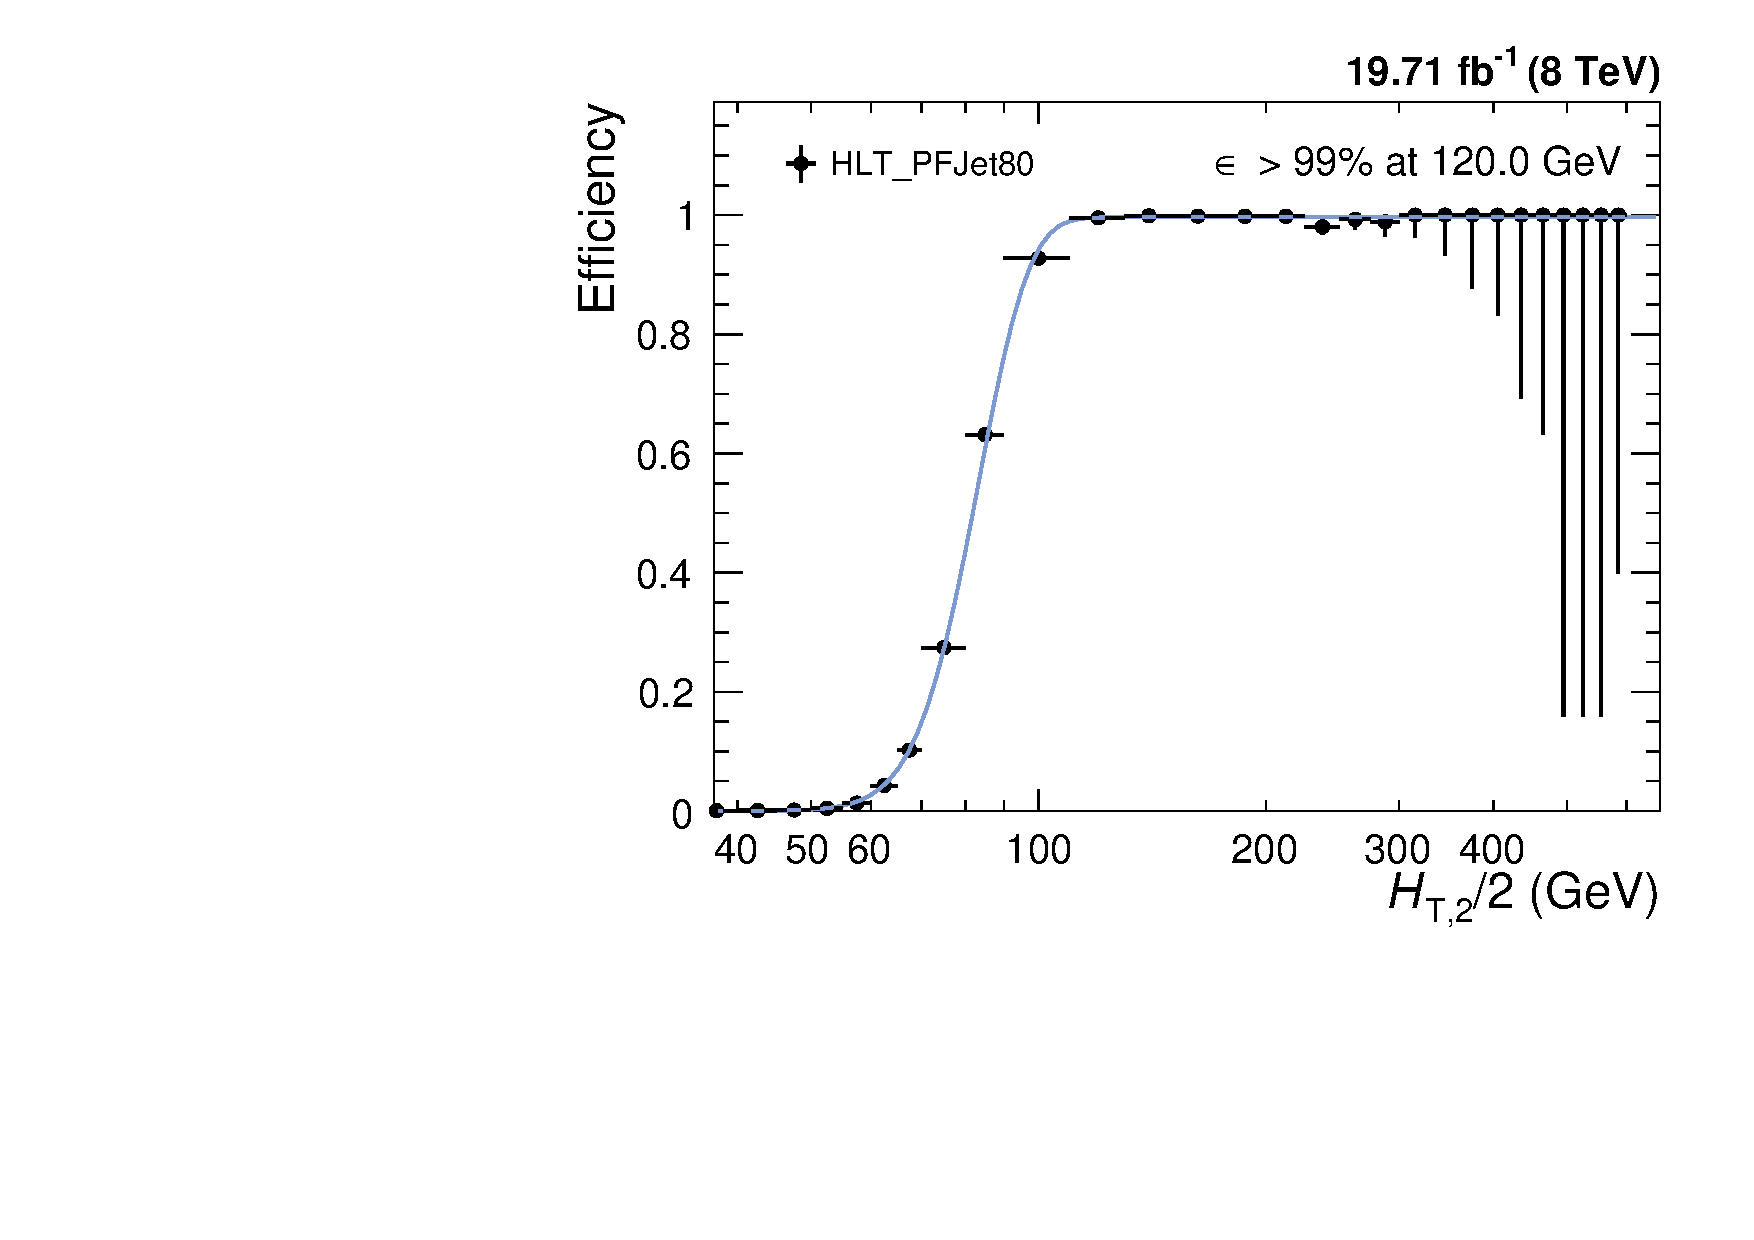
\includegraphics[scale = 0.21]{/home/anter/Desktop/Analysis_8/Present_Latex/Pre-approval/Plots_Final/Fit_Turn_Efficiency_80_2_ht_2.pdf}%
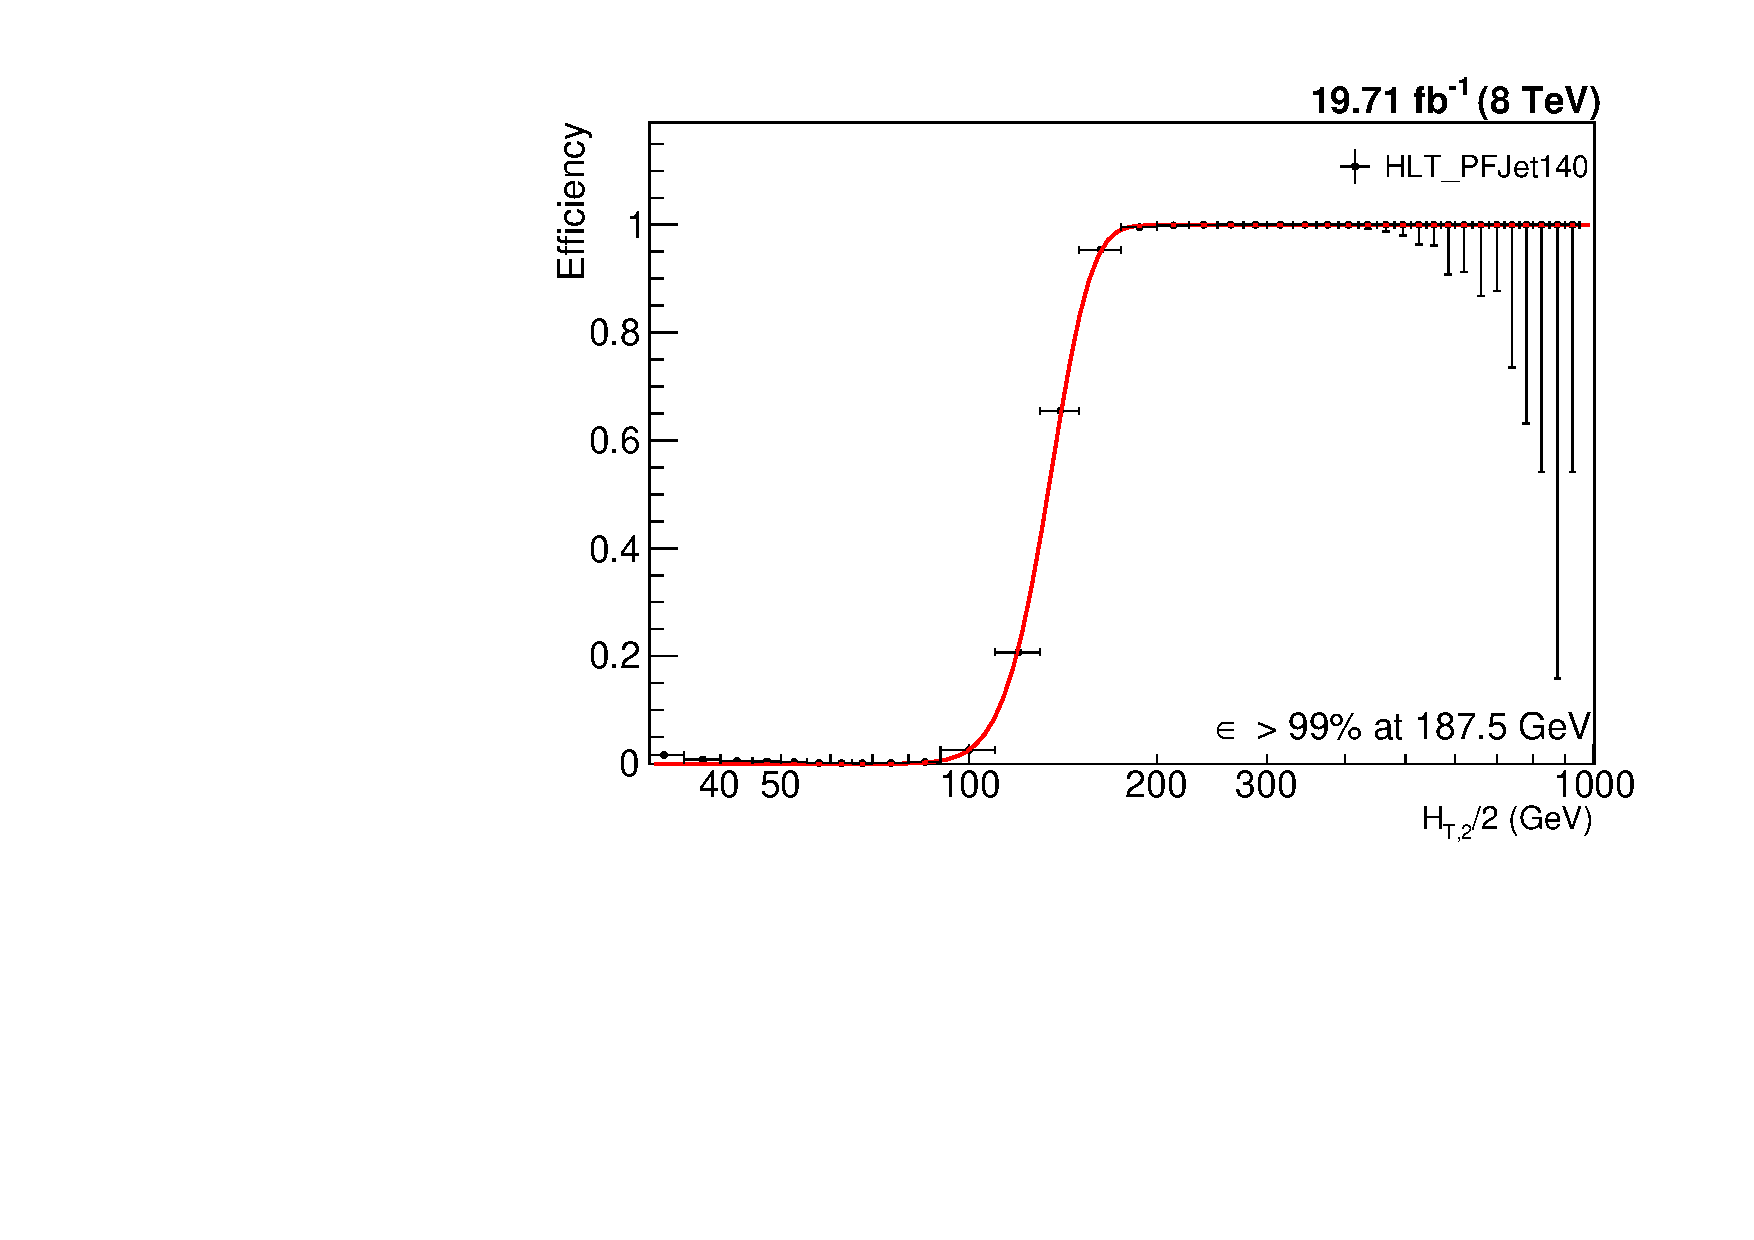
\includegraphics[scale = 0.21]{/home/anter/Desktop/Analysis_8/Present_Latex/Pre-approval/Plots_Final/Fit_Turn_Efficiency_140_2_ht_2.pdf}%
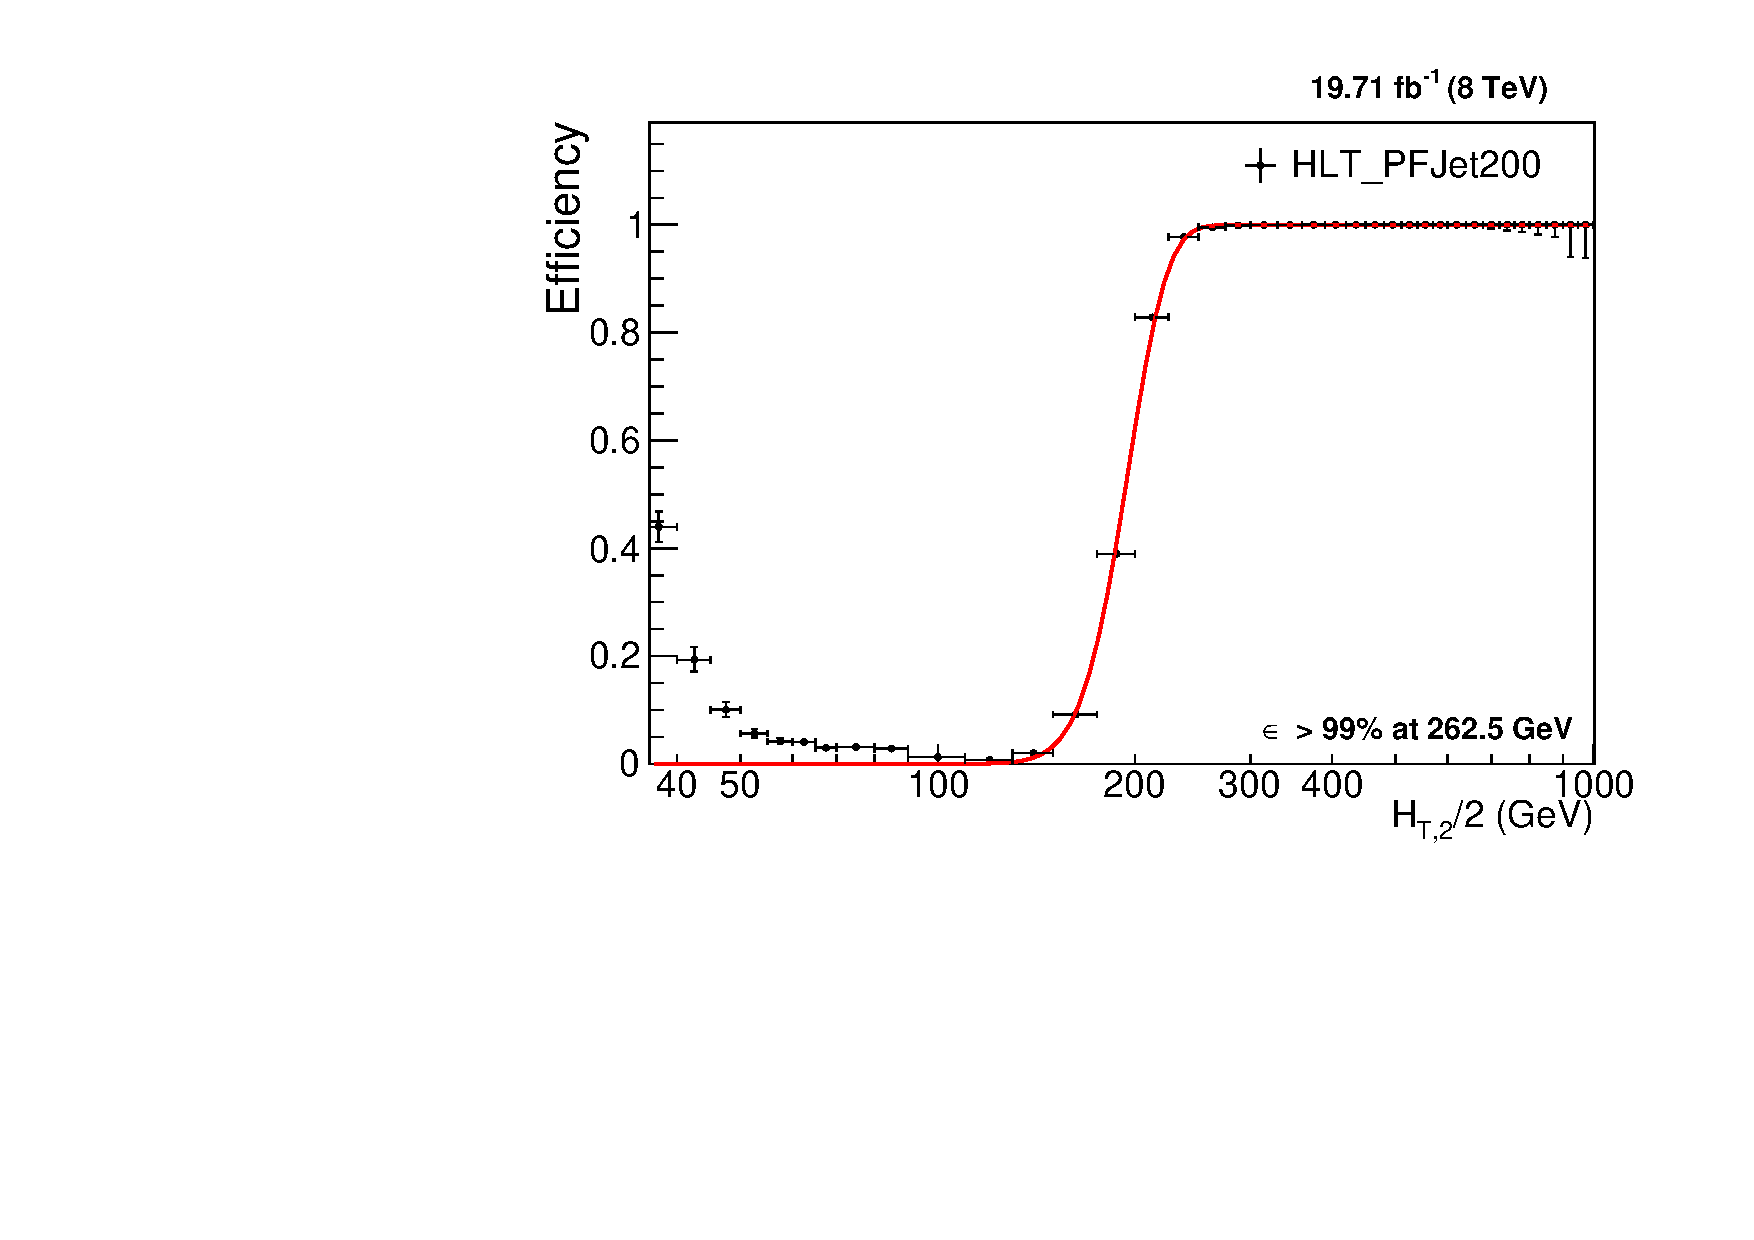
\includegraphics[scale = 0.21]{/home/anter/Desktop/Analysis_8/Present_Latex/Pre-approval/Plots_Final/Fit_Turn_Efficiency_200_2_ht_2.pdf}\\
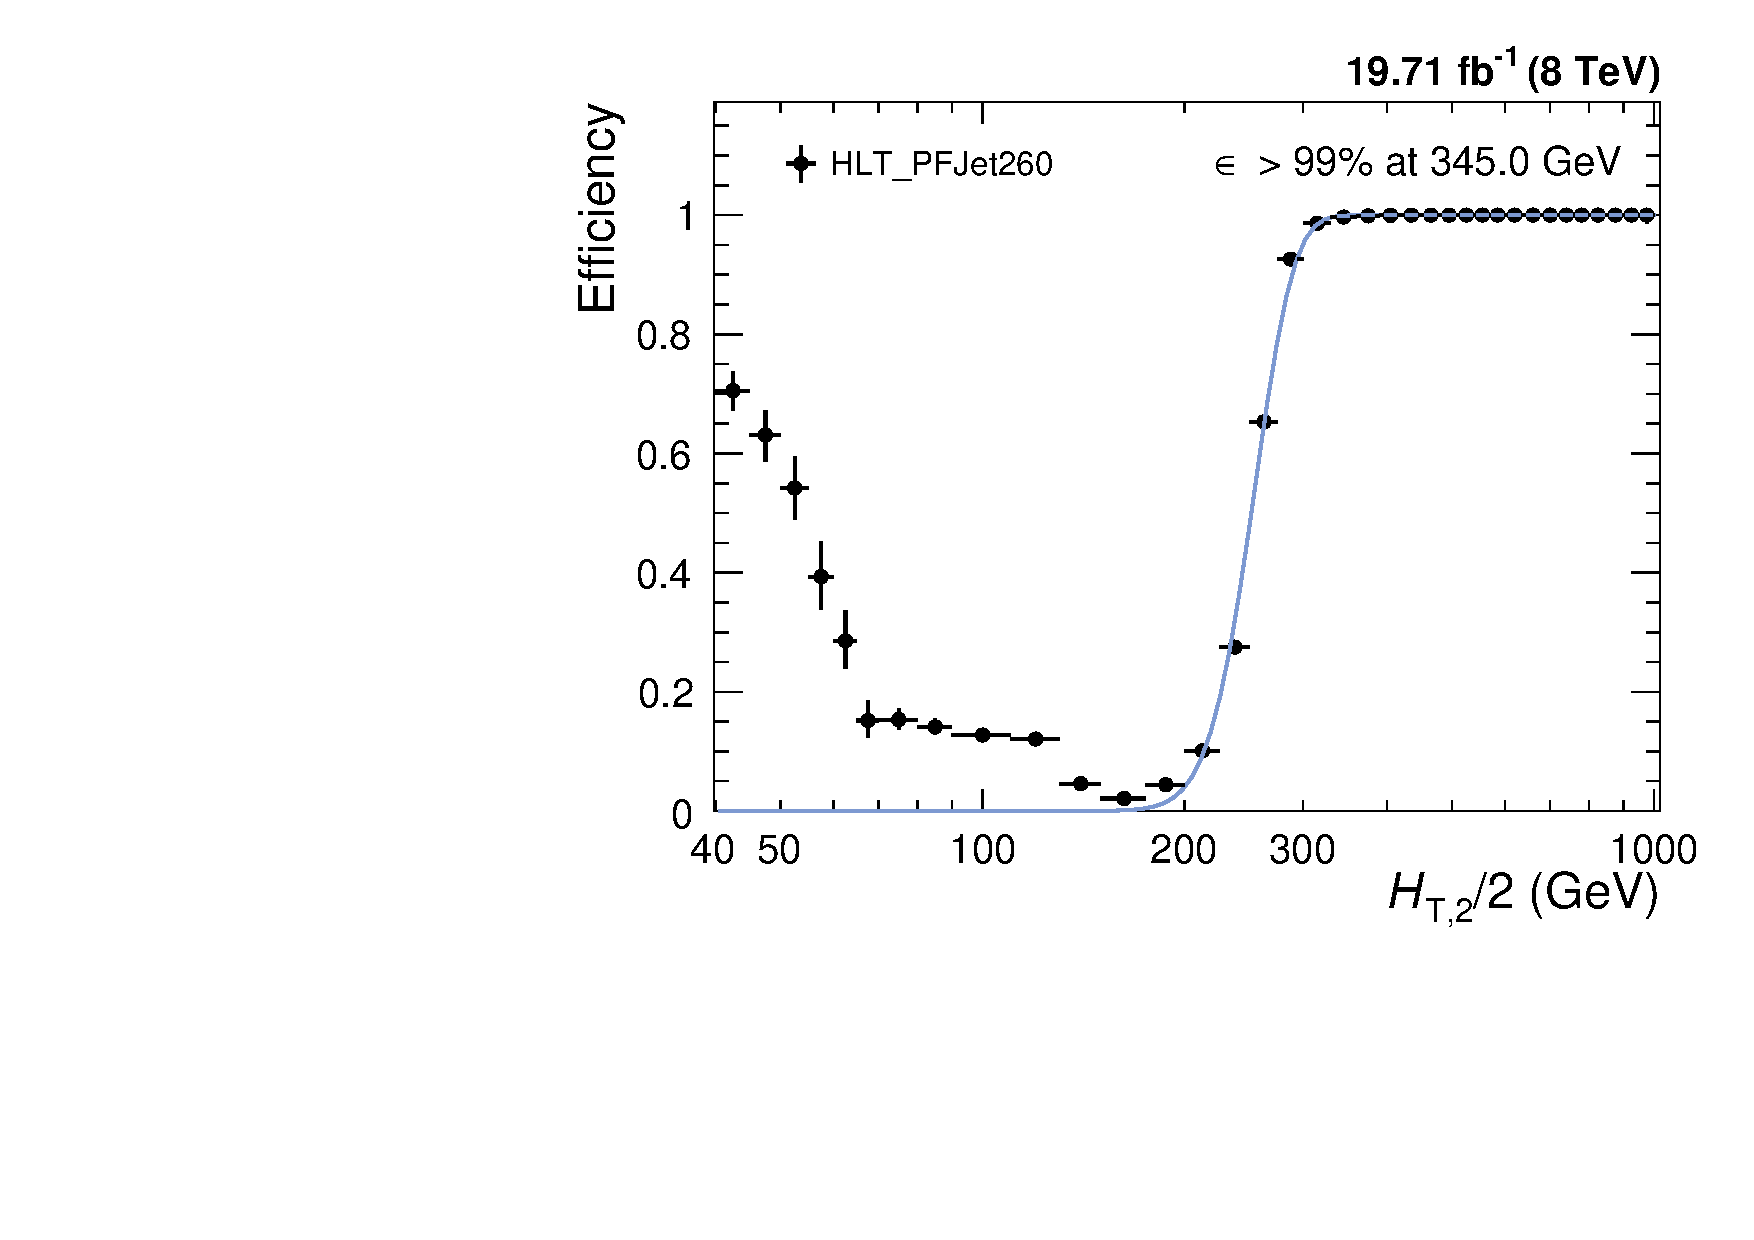
\includegraphics[scale = 0.21]{/home/anter/Desktop/Analysis_8/Present_Latex/Pre-approval/Plots_Final/Fit_Turn_Efficiency_260_2_ht_2.pdf}%
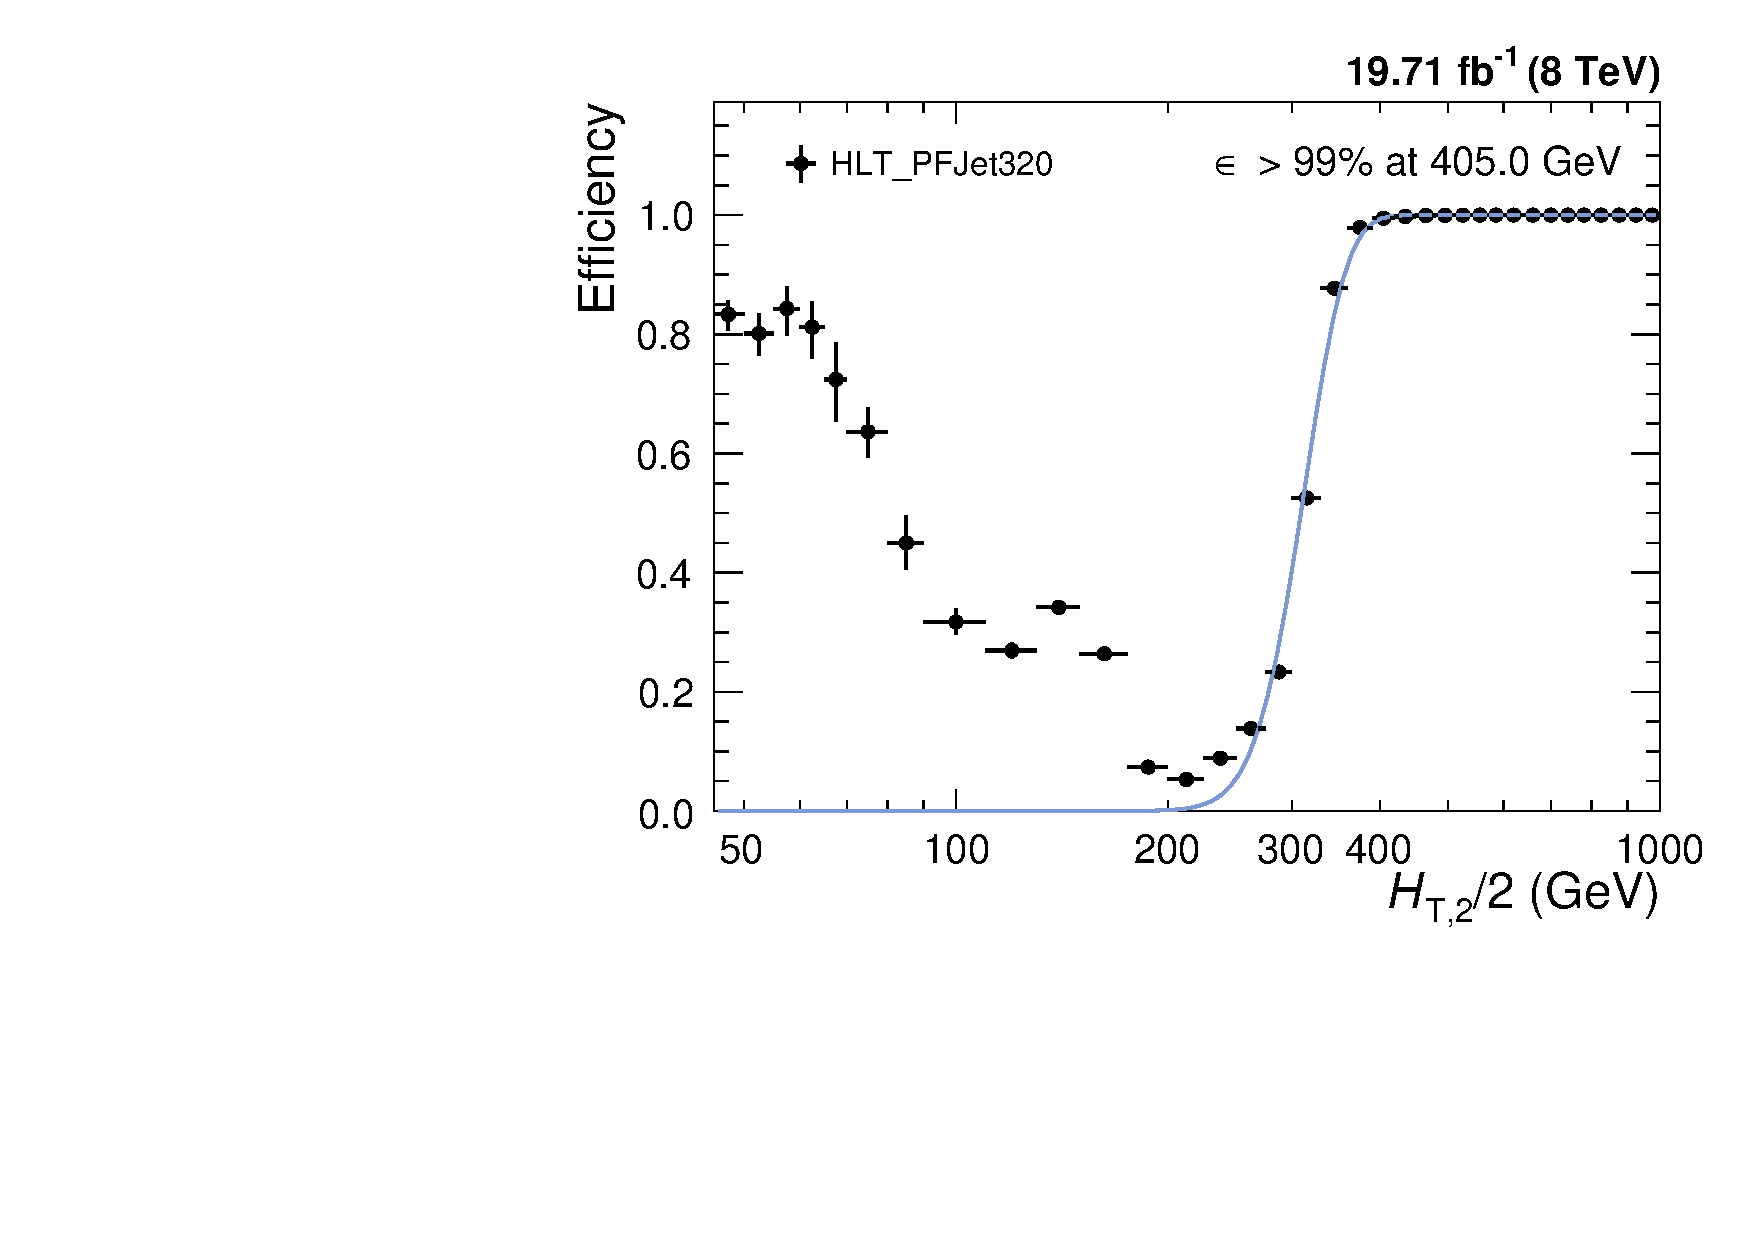
\includegraphics[scale = 0.21]{/home/anter/Desktop/Analysis_8/Present_Latex/Pre-approval/Plots_Final/Fit_Turn_Efficiency_320_2_ht_2.pdf}\\
\end{center}
\end{frame}

%##################################### Slide : 37 ###########################################
%\begin{frame}
%\frametitle{\centerline{ Comparison for Observable}}
%\setlength\labelsep   {\dimexpr\labelsep + 0.05em\relax}
%\setlength\leftmarginiii{\dimexpr\leftmarginiii + 0.05em\relax}
%\vspace{-4mm}
%\begin{center}
%\begin{itemize}
%\item { \footnotesize Monte Carlo distributions are scaled to data with factor w, where}\\
%\vspace{-4mm}
%\begin{align*}
%\resizebox{.60\hsize}{!}{$\rm w = (\sigma_{MC} * \mathcal{L})/N_{MC}$, using $\mathcal{L}$ = 19711.225 pb$^{-1}$} 
%\end{align*}
%\end{itemize}
%\vspace{-3mm}
%\begin{table}[t]
%  \centering\scriptsize
%  \begin{tabular}{|p{1.5cm}|p{2cm}|p{1.5cm}|p{1.5cm}|}
%    \hline
%      MC File & Cross-section ($\rm \sigma_{MC}$) (pb) & Events ($\rm N_{MC}$)  \\\hline
%  
%   100-250 & 10360000.0 & 50127560 \\\hline
%   250-500 & 276000.0 & 27062078  \\\hline
%   50-1000 & 8426.0 & 30543161  \\\hline
%   1000-Inf & 204.0 & 13843863  \\\hline
%  \end{tabular}
% \end{table}
%
%\begin{itemize}
%\vspace{-2mm}
%\item { \footnotesize After this, for Data and MC, the measured yields are transformed to differential cross sections as : }\\
%\vspace{-4mm}
%\begin{align*}
%\resizebox{.30\hsize}{!}{$\rm\frac{d\sigma}{d(H_{T,2}/2)} = \frac{N}{ \mathcal{L} \Delta (H_{T,2}/2)}$}
%\end{align*}
%{ \footnotesize where N is the number of jets in the bin, $\rm \mathcal{L}$ is the integrated luminosity of the data sample i.e. 19711.225 pb$^{-1}$ and $\rm \Delta (H_{T,2}/2)$ is the bin width of scale used.
%\item Comparison of Data is done with theory predictions from NLO and MadGraph\plus Pythia6 MC samples.}\\
%\end{itemize}
%\end{center}
%\end{frame}

%##################################### Slide : 38 ###########################################
\begin{frame}
\frametitle{\centerline{Detector-Level Comparison of Cross Sections}}
\setlength\labelsep   {\dimexpr\labelsep + 0.05em\relax}
\setlength\leftmarginiii{\dimexpr\leftmarginiii + 0.05em\relax}

\begin{center}
\begin{itemize}
\vspace{-4mm}
\item {\scriptsize Binning used is inherited from R$_{32}$ at 7 TeV : 150., 175., 200., 225., 250., 275., 300., 330., 360., 390., 420., 450., 480., 510., 540., 570., 600., 640., 680., 720., 760., 800., 850., 900., 950., 1000., 1060., 1120., 1180., 1250., 1320., 1390., 1460., 1530., 1600., 1680., 1760., 1840., 1920., 2000.
\item Comparison of 2012 full data is done with NLO predictions as well as MG\plus P6 MC Simulations.
\item 150-200 bins are not included to avoid the infrared sensitivity for the bins next to min. \pt cut in NLO calculations for events with inclusive 2\mbox{-}jet events. \\}
\end{itemize}
\vspace{3mm}
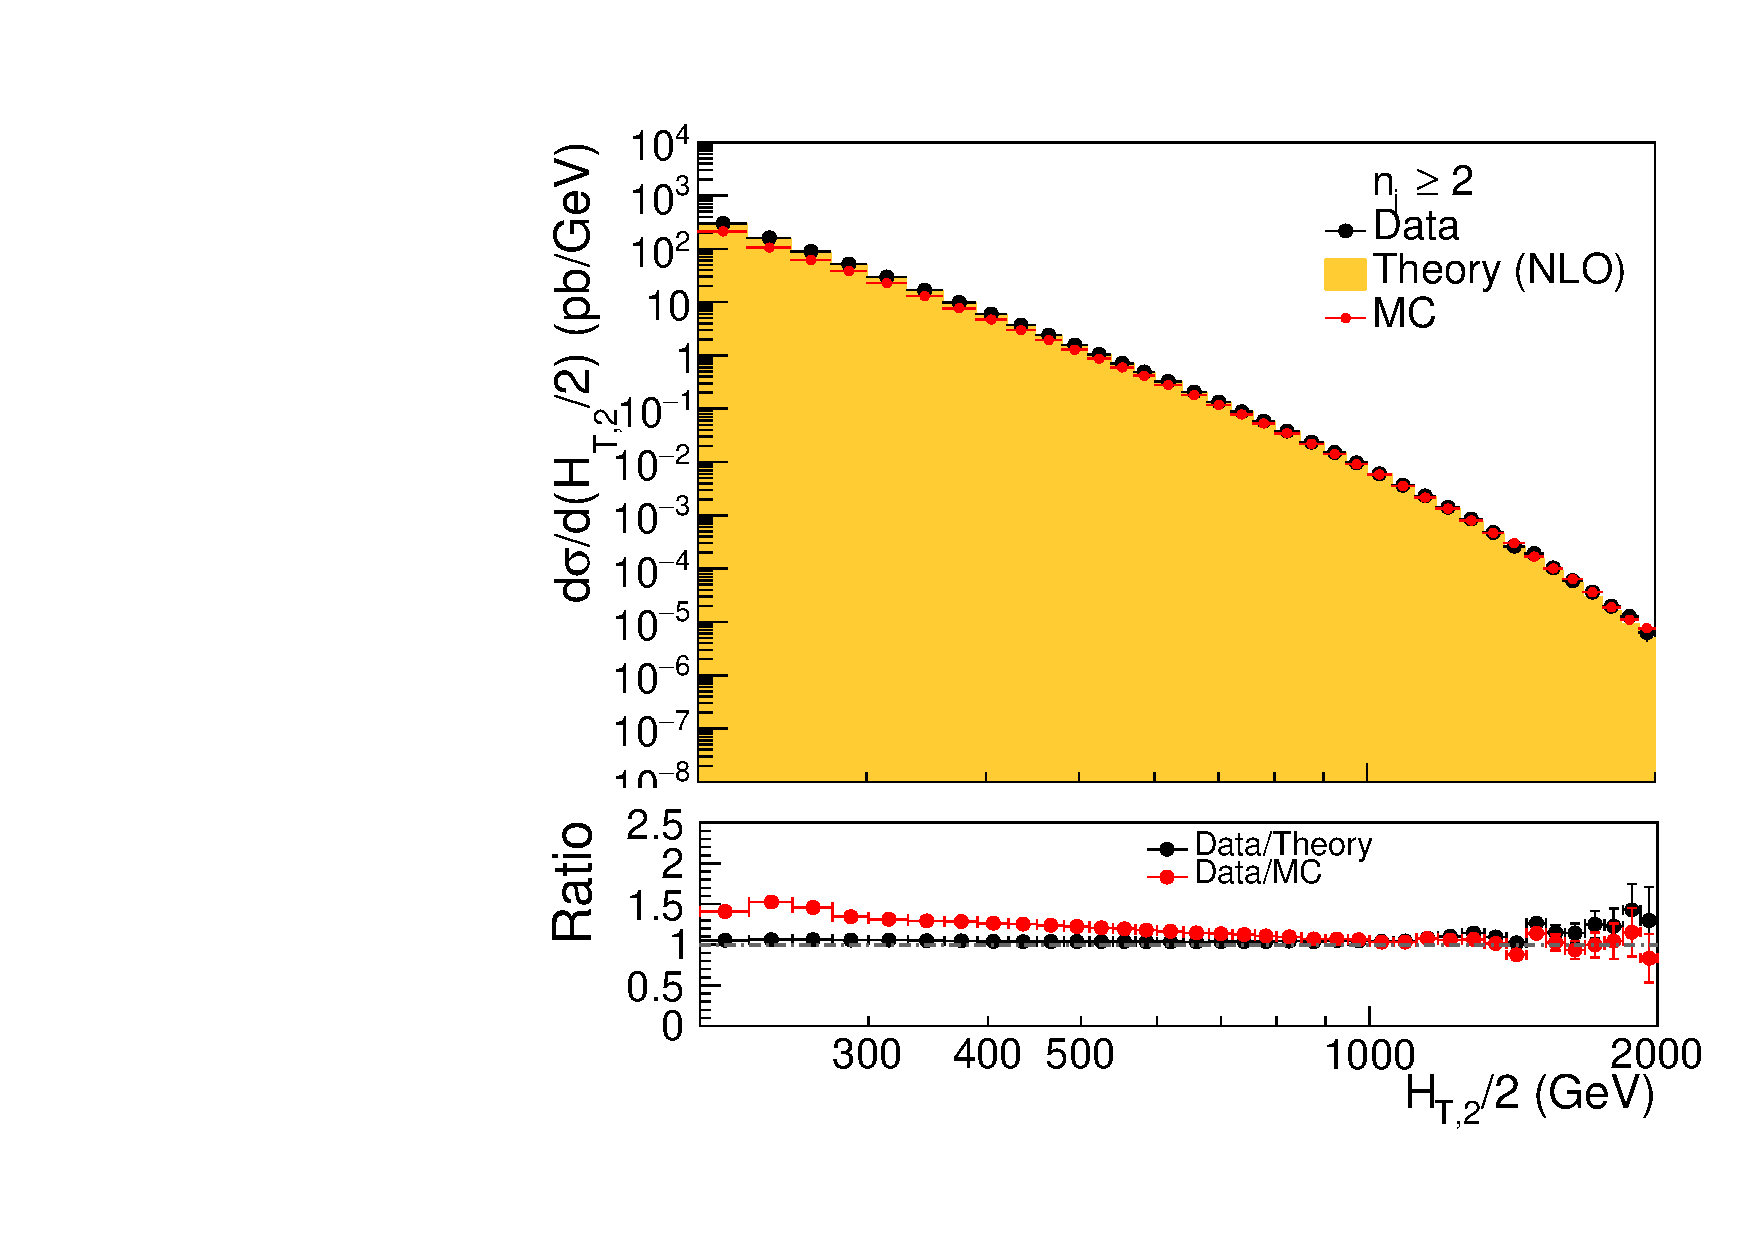
\includegraphics[scale = 0.205]{/home/anter/Desktop/Analysis_8/Present_Latex/Pre-approval/Plots/Comparison_all_2_HT_2_150.pdf}%
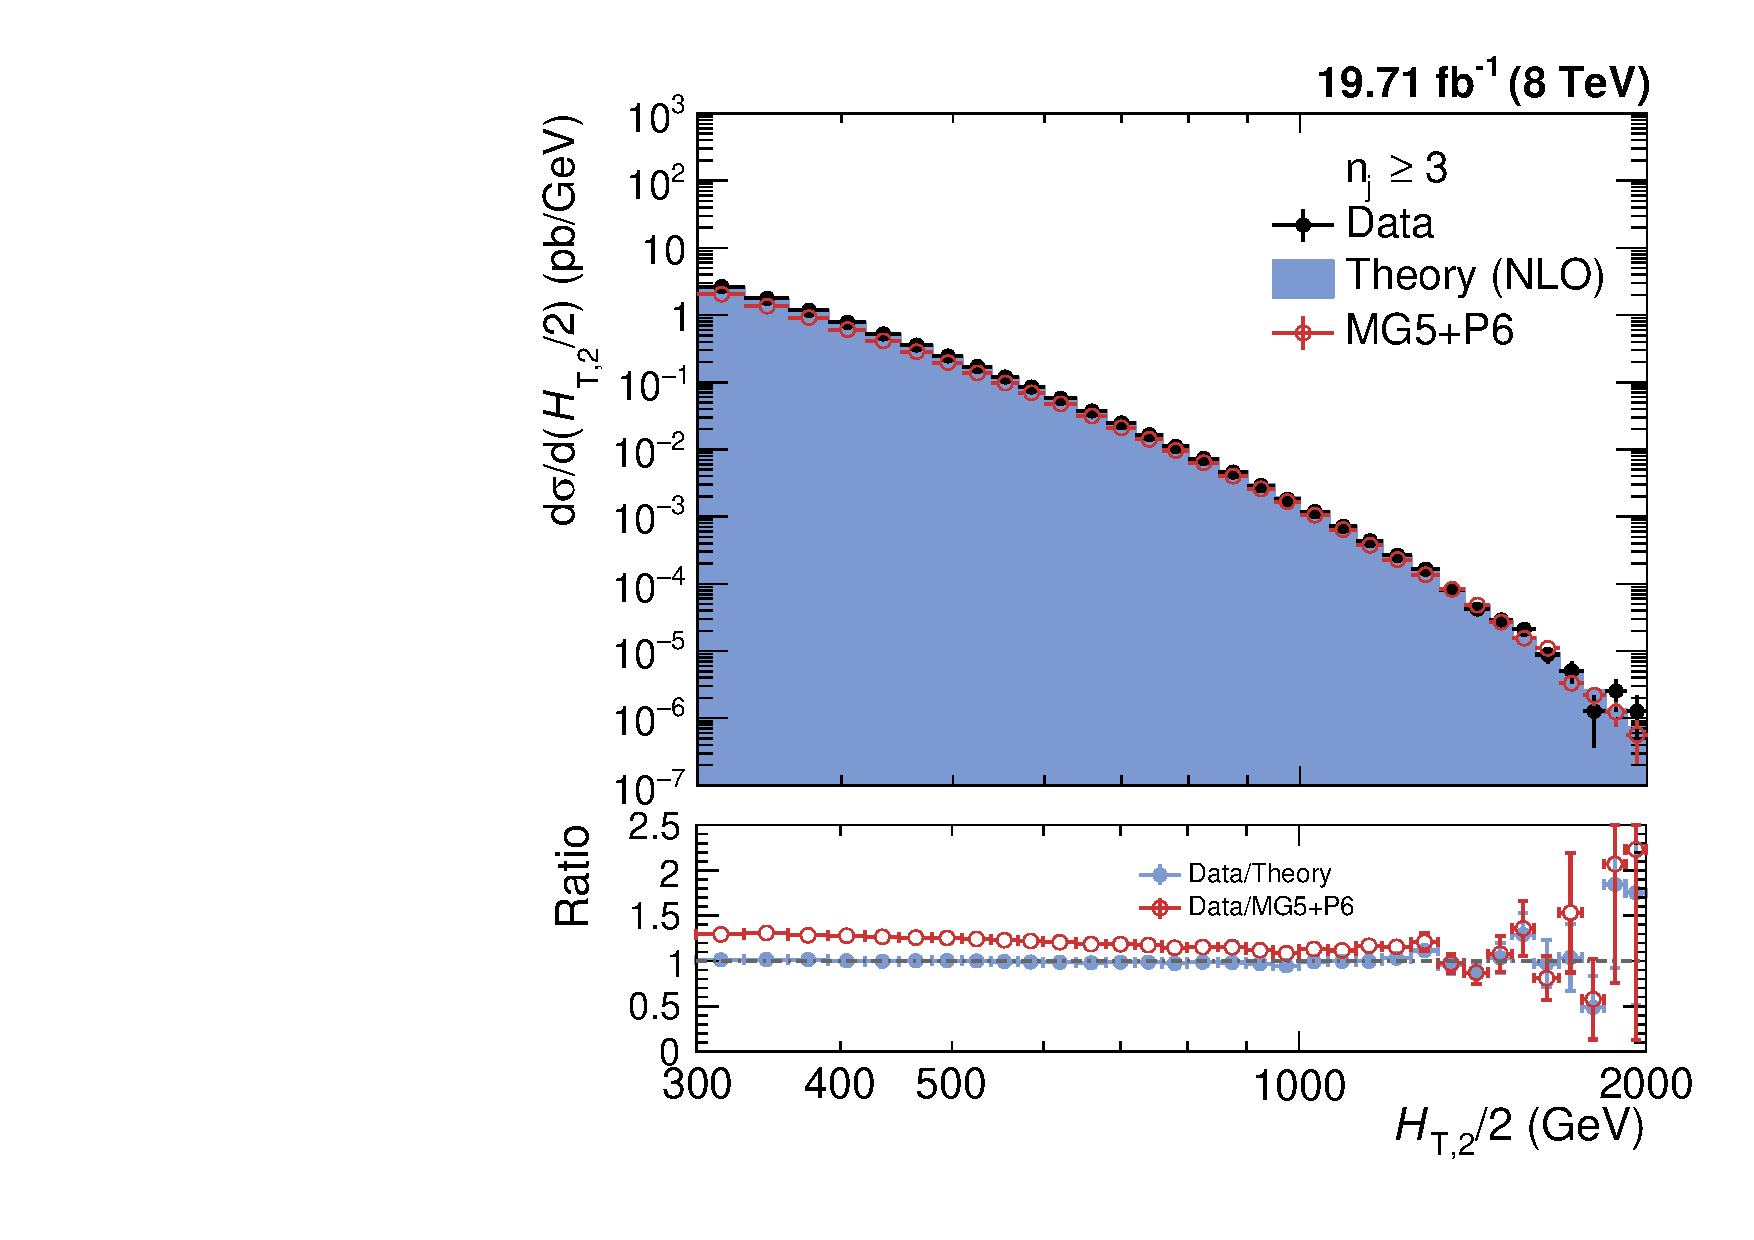
\includegraphics[scale = 0.205]{/home/anter/Desktop/Analysis_8/Present_Latex/Pre-approval/Plots/Comparison_all_3_HT_2_150.pdf}%
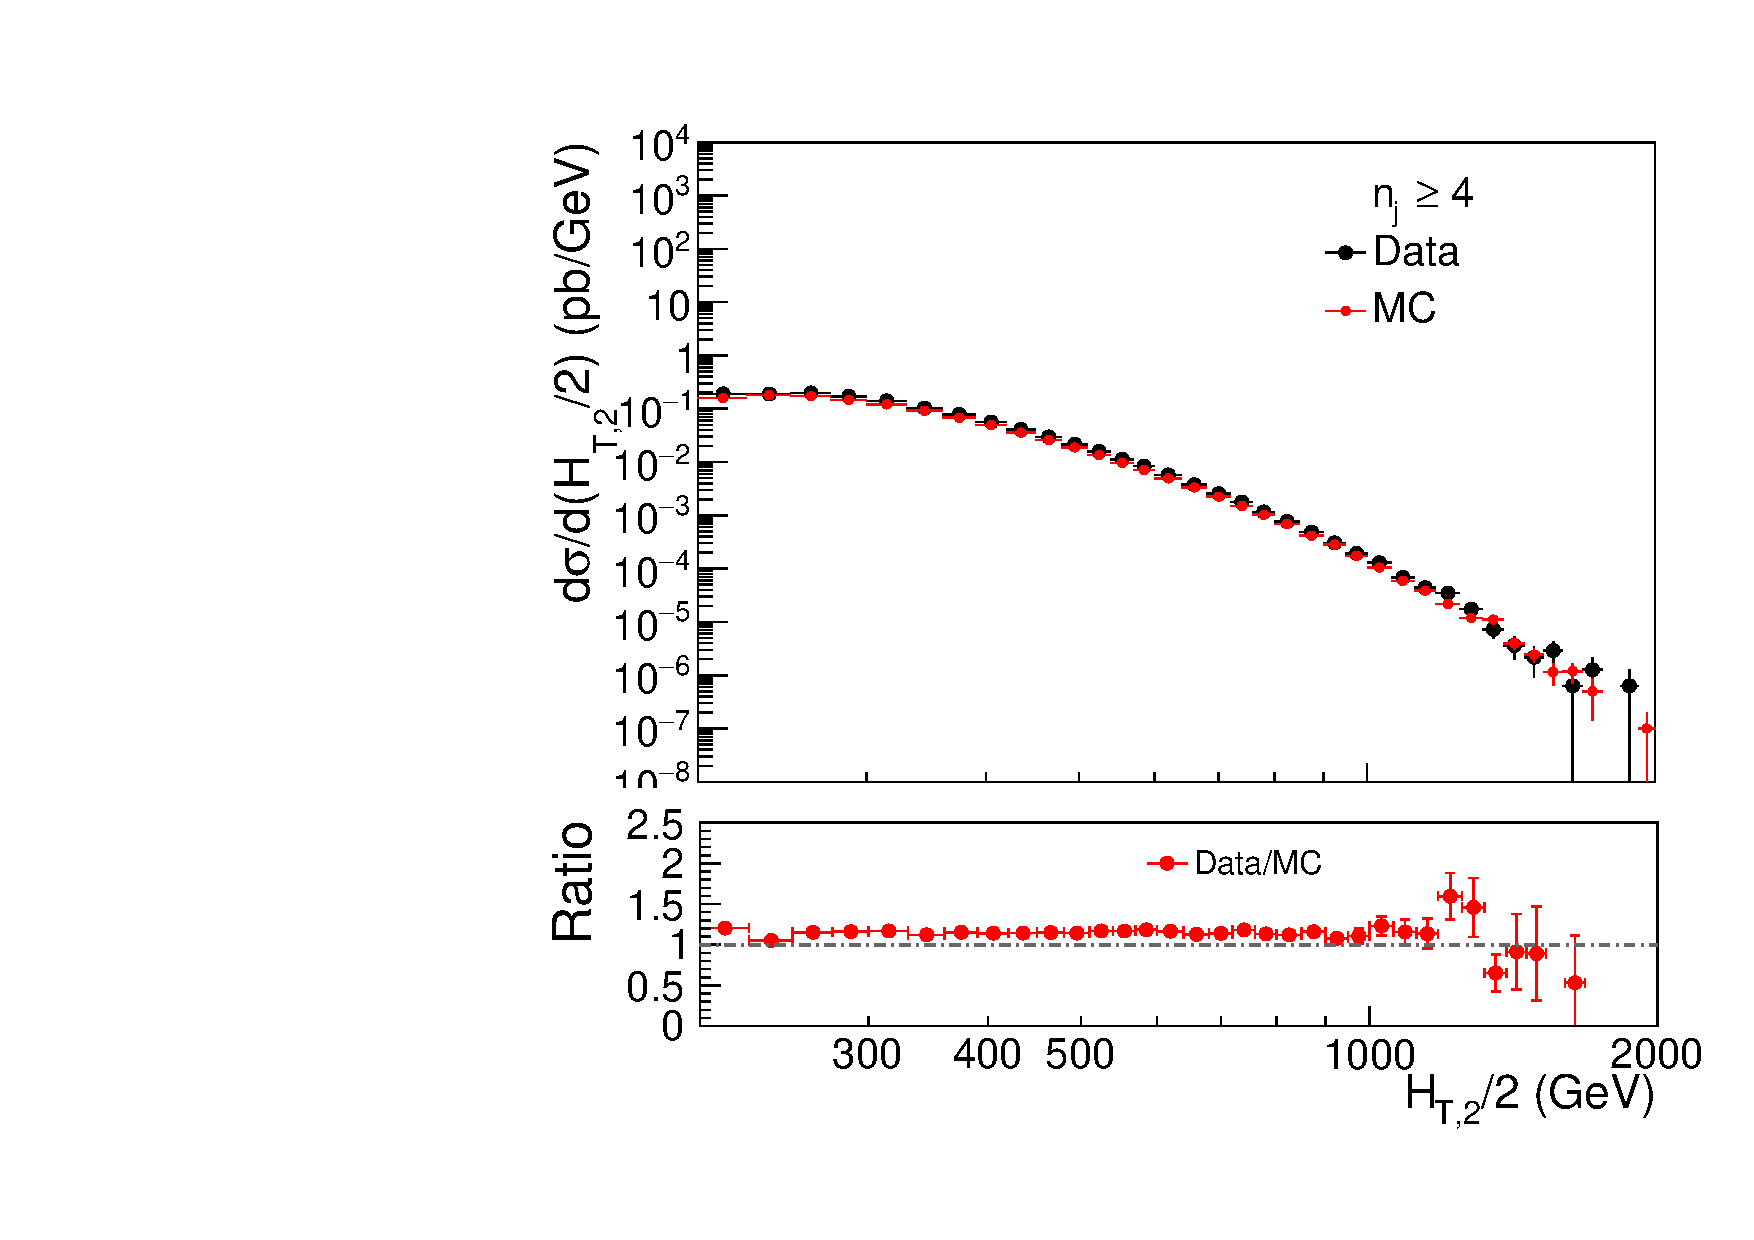
\includegraphics[scale = 0.205]{/home/anter/Desktop/Analysis_8/Present_Latex/Pre-approval/Plots/Comparison_all_4_HT_2_150.pdf}\\
\end{center}
\mycolor {$^{\star}$\scriptsize NLO theory predictions are yet to be done for inclusive 4\mbox{-}jet events.\\ }
\end{frame}

%##################################### Slide : 41 ###########################################
\begin{frame}
\label{fit_formula}
\frametitle{\centerline{Unfolding : Fitting NLO predictions }}
\setlength\labelsep   {\dimexpr\labelsep + 0.05em\relax}  
\setlength\leftmargini{\dimexpr\leftmargini + 0.05em\relax}
\vspace{-3mm}
\begin{center}
\begin{itemize}
\item {\tiny Fitting the NLO $\rm{H_{T,2}/2}$ spectrum by the function \mycolor{(Function I)} \\}
\vspace{-7mm}
\begin{align*}
\resizebox{.38\hsize}{!}{$\rm{f(p_{T}) = N[x_{T}]^{-a}[1-x_{T}]^{b} \times exp[-c/x_{T}]}$}
\end{align*}
{\tiny where N is normalization factor and a, b, c are fit parameters.\\ }
\vspace{2mm}\tri
\begin{itemize}
\item {\tiny This function is derived from the below function from \textbf {``Measurement of the Inclusive Jet Cross Section in pp Collisions at $\sqrt{s}$=7 TeV'' (Phys.Rev.Lett. 107, 132001 (2011))}\\ }
\end{itemize}
\hspace{30mm} 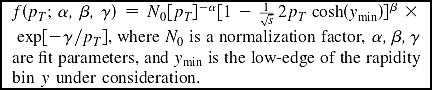
\includegraphics[scale = 0.45]{/home/anter/Desktop/Analysis_8/Present_Latex/Klaus/2016/2_February/Fit_plots/Formula.png} 
\begin{itemize}
{ \tiny using \\ }
\end{itemize}
\vspace{-6mm}
\begin{align*}
\resizebox{.22\hsize}{!}{$\rm{\alpha = a,~~\beta = b,~~\gamma = c*\sqrt{s}/2},$} \\ 
\resizebox{.22\hsize}{!}{$\rm{x_{T} = \frac{2*p_{T}*cosh(y_{min})}{\sqrt{s}}} \rm{= \frac{2*p_{T}}{\sqrt{s}}}$}
\end{align*}
\begin{itemize}
\vspace{-5mm}
{\tiny where transverse scaling variable $\rm{x_{T}}$ corresponds to the proton fractional momentum x for dijets with rapidity y=0, $\rm{\sqrt{s}}$ = 8000 GeV and $\rm{y_{min}}$ is low-edge of the rapidity bin y under consideration (Here $\rm{y_{min}}$ is taken equal to 0) \\}
\end{itemize}
\end{itemize}
\vspace{2mm}\ball
\begin{itemize}
{ \tiny \item Fitting the NLO $\rm{H_{T,2}/2}$ spectrum by the function \mycolor{(Function II)} (\textbf{CMS AN-12-223}) :
\begin{align*}
\rm{f(H_{T,2}/2) = A_{0}\Big(1-\frac{H_{T,2}/2}{A_{6}}\Big)^{A_{7}} \times 10^{F(x)}}, \rm where ~~~{F(x) = \sum\limits_{i=1}^5 A_{i}\Big(log\big(\frac{x}{A_{6}}\big)\Big)^{i}}~~~~~~~~~~~~~~~
\end{align*}
where the parameter $\rm{A_{6}}$ is fixed to $\rm{\frac{\sqrt{s}}{2cosh(y_{min})}}$, where $\rm{\sqrt{s}}$ = 8000 GeV and $\rm{y_{min}}$ is the minimum rapidity. The other parameters are derived from the fitting.\\ }
\end{itemize}
\end{center}
\end{frame}

%##################################### Slide : 13 ###########################################
\begin{frame}
\frametitle{\centerline{Unfolding : Fitting NLO predictions }}
\setlength\labelsep   {\dimexpr\labelsep + 0.05em\relax}
\setlength\leftmargini{\dimexpr\leftmargini + 0.05em\relax}
\vspace{-3mm}
\begin{center}
\begin{itemize}
\item {\scriptsize First fit the NLO spectrum with function in the range (specified on the plot) and then using the obtained fit parameters extrapolated it to lower value.\\}
\end{itemize}
{\scriptsize \textbf {\mycolor{Function I (Left) and Function II (Right)}}}\\
\includegraphics[scale = 0.25]{/home/anter/Desktop/Analysis_8/Present_Latex/Pre-approval/Plots/Extrapolate_Theory_2_HT_2_150.pdf}%
\includegraphics[scale = 0.25]{/home/anter/Desktop/Analysis_8/Present_Latex/Pre-approval/Plots/Extrapolate_Theory_2_HT_2_150_old.pdf}\\
\includegraphics[scale = 0.25]{/home/anter/Desktop/Analysis_8/Present_Latex/Pre-approval/Plots/Extrapolate_Theory_3_HT_2_150.pdf}%
\includegraphics[scale = 0.25]{/home/anter/Desktop/Analysis_8/Present_Latex/Pre-approval/Plots/Extrapolate_Theory_3_HT_2_150_old.pdf}
\end{center}
\end{frame}

%##################################### Slide : 15 ###########################################
\begin{frame}
\frametitle{\centerline{Unfolding (from MG\plus P6)}}
\setlength\labelsep   {\dimexpr\labelsep + 0.05em\relax}
\setlength\leftmarginiii{\dimexpr\leftmarginiii + 0.05em\relax}
\vspace{-6.5mm}
\begin{center}
{\scriptsize \textbf {Inclusive-2 jet~~~\hspace{20mm}Inclusive-3 jet~~~\hspace{20mm}Inclusive 4\mbox{-}jet}}
\vspace{-3mm}
\includegraphics[scale = 0.205]{/home/anter/Desktop/Analysis_8/Present_Latex/Pre-approval/Plots/Normalized_Response_Matrix_Madgraph_2_HT_2_150.pdf}%
\includegraphics[scale = 0.205]{/home/anter/Desktop/Analysis_8/Present_Latex/Pre-approval/Plots/Normalized_Response_Matrix_Madgraph_3_HT_2_150.pdf}%
\includegraphics[scale = 0.205]{/home/anter/Desktop/Analysis_8/Present_Latex/Pre-approval/Plots/Normalized_Response_Matrix_Madgraph_4_HT_2_150.pdf}\\
\includegraphics[scale = 0.205]{/home/anter/Desktop/Analysis_8/Present_Latex/Pre-approval/Plots/Ratio_Unfolding_theory_Mad_2_HT_2_150.pdf}%
\includegraphics[scale = 0.205]{/home/anter/Desktop/Analysis_8/Present_Latex/Pre-approval/Plots/Ratio_Unfolding_theory_Mad_3_HT_2_150.pdf}%
\includegraphics[scale = 0.205]{/home/anter/Desktop/Analysis_8/Present_Latex/Pre-approval/Plots/Ratio_Unfolding_theory_Mad_4_HT_2_150.pdf}\\
\vspace{-2mm}
\includegraphics[scale = 0.205]{/home/anter/Desktop/Analysis_8/Present_Latex/Pre-approval/Plots/Ratio_Unfolding_data_Mad_2_HT_2_150.pdf}%
\includegraphics[scale = 0.205]{/home/anter/Desktop/Analysis_8/Present_Latex/Pre-approval/Plots/Ratio_Unfolding_data_Mad_3_HT_2_150.pdf}%
\includegraphics[scale = 0.205]{/home/anter/Desktop/Analysis_8/Present_Latex/Pre-approval/Plots/Ratio_Unfolding_data_Mad_4_HT_2_150.pdf}\\
\end{center}
\end{frame}

%##################################### Slide : 16 ###########################################
\begin{frame}
\label{corr}
\frametitle{\centerline{Unfolding : Correlation Matrices (NLO)}}
\setlength\labelsep   {\dimexpr\labelsep + 0.05em\relax}
\setlength\leftmarginiii{\dimexpr\leftmarginiii + 0.05em\relax}
\vspace{-4mm}
\begin{center}
{\scriptsize \textbf {Inclusive 2\mbox{-}jet (Top) and Inclusive 3\mbox{-}jet (Bottom)}}\\
\vspace{2mm}
{\scriptsize \textbf {\hspace{2mm}4 Iterations\hspace{29mm}5 Iterations\hspace{26mm}10 Iterations}}\\
\vspace{2mm}
\includegraphics[scale = 0.205]{/home/anter/Desktop/Analysis_8/Present_Latex/Approval/Approval/Correlation_Matrix_NLO_2_ite4.pdf}%
\includegraphics[scale = 0.205]{/home/anter/Desktop/Analysis_8/Present_Latex/Approval/Approval/Correlation_Matrix_NLO_2_ite5.pdf}%
\includegraphics[scale = 0.205]{/home/anter/Desktop/Analysis_8/Present_Latex/Approval/Approval/Correlation_Matrix_NLO_2_ite10.pdf}\\
\includegraphics[scale = 0.205]{/home/anter/Desktop/Analysis_8/Present_Latex/Approval/Approval/Correlation_Matrix_NLO_3_ite4.pdf}%
\includegraphics[scale = 0.205]{/home/anter/Desktop/Analysis_8/Present_Latex/Approval/Approval/Correlation_Matrix_NLO_3_ite5.pdf}%
\includegraphics[scale = 0.205]{/home/anter/Desktop/Analysis_8/Present_Latex/Approval/Approval/Correlation_Matrix_NLO_3_ite10.pdf}\\
\end{center}
\end{frame}

%##################################### Slide : 16 ###########################################
\begin{frame}
\frametitle{\centerline{Unfolding : Correlation Matrices (MG\plus P6)}}
\setlength\labelsep   {\dimexpr\labelsep + 0.05em\relax}
\setlength\leftmarginiii{\dimexpr\leftmarginiii + 0.05em\relax}
\vspace{-6mm}
\begin{center}
{\tiny \textbf {Inclusive 2\mbox{-}jet (Top), Inclusive 3\mbox{-}jet (Middle) and Inclusive 4\mbox{-}jet (Bottom)}}\\
\vspace{-2mm}
{\tiny \textbf {\hspace{2mm}4 Iterations\hspace{22mm}5 Iterations\hspace{20mm}10 Iterations}}\\
\includegraphics[scale = 0.165]{/home/anter/Desktop/Analysis_8/Present_Latex/Pre-approval/Plots/Correlation_Matrix_Mad_2_ite4.pdf}%
\includegraphics[scale = 0.165]{/home/anter/Desktop/Analysis_8/Present_Latex/Pre-approval/Plots/Correlation_Matrix_Mad_2_ite5.pdf}%
\includegraphics[scale = 0.165]{/home/anter/Desktop/Analysis_8/Present_Latex/Pre-approval/Plots/Correlation_Matrix_Mad_2_ite10.pdf}\\
\includegraphics[scale = 0.165]{/home/anter/Desktop/Analysis_8/Present_Latex/Pre-approval/Plots/Correlation_Matrix_Mad_3_ite4.pdf}%
\includegraphics[scale = 0.165]{/home/anter/Desktop/Analysis_8/Present_Latex/Pre-approval/Plots/Correlation_Matrix_Mad_3_ite5.pdf}%
\includegraphics[scale = 0.165]{/home/anter/Desktop/Analysis_8/Present_Latex/Pre-approval/Plots/Correlation_Matrix_Mad_3_ite10.pdf}\\
\includegraphics[scale = 0.165]{/home/anter/Desktop/Analysis_8/Present_Latex/Pre-approval/Plots/Correlation_Matrix_Mad_4_ite4.pdf}%
\includegraphics[scale = 0.165]{/home/anter/Desktop/Analysis_8/Present_Latex/Pre-approval/Plots/Correlation_Matrix_Mad_4_ite5.pdf}%
\includegraphics[scale = 0.165]{/home/anter/Desktop/Analysis_8/Present_Latex/Pre-approval/Plots/Correlation_Matrix_Mad_4_ite10.pdf}\\
\end{center}
\end{frame}

%##################################### Slide : 12 ###########################################
\begin{frame}
\label{closure}
  \frametitle{\centerline{Closure tests}}
  \setlength\labelsep   {\dimexpr\labelsep + 0.05em\relax}
  \setlength\leftmarginiii{\dimexpr\leftmarginiii + 0.05em\relax}
  \vspace{-1.5mm}
  \begin{itemize}
   \item {\tiny \blue  {Blue curve} \\}
   \tri
   \begin{itemize}
   \item {\tiny  Simulated MG\plus P6 Reco/MG\plus P6 Gen
   \vspace{0.2mm}   
   \item Resolution (Res.) is extracted from this simulation \\}
   \end{itemize}
   \vspace{-1.mm}    
   \ball
   \item {\tiny \mycolor {Red curve} \\}
   \tri
   \begin{itemize}
   \item {\tiny  Extracted Res. smears FastNLO too much, in a vey large y bin
   \vspace{0.2mm}   
   \item ARC agreed to add this non-closure as additional uncertainty for now\\}
   \end{itemize}
   \ball
   \vspace{-1.mm}
   \item {\tiny Black dashed curve \\}
   \tri
   \begin{itemize}
   \item {\tiny Proves that the extracted Res. also smears MG\plus P6 Gen more \\}
   \end{itemize}
   \ball
   \vspace{-1.mm}
   \item {\tiny \textcolor{pink} {Magenta curve}\\}
   \tri
   \begin{itemize}
   \item {\tiny Closure with \blue{blue curve} when 30\% reduced Res. is used to smear MG\plus P6 Gen \\}
   \end{itemize}
   \ball
   \vspace{-1.mm}
   \item {\tiny \green {Green curve} \\}
   \tri
   \begin{itemize}
   \item {\tiny Closure with \blue{blue curve} when FastNLO is smeared using 30\% reduced Res.
   \vspace{0.1mm}
   \item An additional uncertainty is attributed by comparison to an unfolding with a 30\% reduced Res. with the one using extracted Res.\\}
   \end{itemize}
   \ball
  \end{itemize}
  \vspace{-2mm}
  \begin{center}
\includegraphics[scale = 0.29]{/home/anter/Desktop/Analysis_8/Present_Latex/After_Pre-approval/New_Plots_PAS/Ratio_all_2_crystal.pdf}%
\includegraphics[scale = 0.29]{/home/anter/Desktop/Analysis_8/Present_Latex/After_Pre-approval/New_Plots_PAS/Ratio_all_3_crystal.pdf}\\

\end{center}
\end{frame}

%##################################### Slide : 16 ###########################################
\begin{frame}
\frametitle{\centerline{Unfolding \ratio}}
\setlength\labelsep   {\dimexpr\labelsep + 0.05em\relax}
\setlength\leftmarginiii{\dimexpr\leftmarginiii + 0.05em\relax}
\vspace{-4mm}
\begin{center}
\vspace{2mm}
\begin{itemize}
\item {\scriptsize {\bf Correlation Matrices (NLO)} \\}
\end{itemize}
{\scriptsize \textbf {\hspace{2mm}4 Iterations\hspace{29mm}5 Iterations\hspace{26mm}10 Iterations}}\\
\vspace{2mm}
\includegraphics[scale = 0.205]{/home/anter/Desktop/Analysis_8/Present_Latex/Approval/Approval/Correlation_Matrix_NLO_Ratio_32_ite4.pdf}%
\includegraphics[scale = 0.205]{/home/anter/Desktop/Analysis_8/Present_Latex/Approval/Approval/Correlation_Matrix_NLO_Ratio_32_ite5.pdf}%
\includegraphics[scale = 0.205]{/home/anter/Desktop/Analysis_8/Present_Latex/Approval/Approval/Correlation_Matrix_NLO_Ratio_32_ite10.pdf}\\
\begin{itemize}
\item {\scriptsize {\bf Unfolding \ratio} \\}
\end{itemize}
\vspace{-5mm}
\includegraphics[scale = 0.27]{/home/anter/Desktop/Analysis_8/Present_Latex/Approval/Approval_New/Comparison_ratio_32_direct_unfolded_smear2.pdf}
\end{center}
\end{frame}

%##################################### Slide : 20 ###########################################
\begin{frame}
\frametitle{\centerline{JES Uncertainty in $\rm \frac{H_{T,2}}{2}$}}
\setlength\labelsep   {\dimexpr\labelsep + 0.05em\relax}
\setlength\leftmarginiii{\dimexpr\leftmarginiii + 0.05em\relax}
\begin{center} 
\vspace{-3mm} 
\begin{itemize}
\item {\scriptsize {\bf Jet Energy Scale (JES)} \\}
\tri
\begin{itemize}
\item { \scriptsize 24 JES mutually uncorrelated uncertainty sources (Winter14\_V8) are considered :\\ }
\begin{itemize}
\setbeamertemplate{itemize items}[square]
\item { \tiny AbsoluteStat, AbsoluteScale, AbsoluteMPFBias, 
\vspace{1mm}
\item Fragmentation, SinglePionECAL, SinglePionHCAL, FlavorQCD,
\vspace{1mm}
\item RelativeJEREC1, RelativeJEREC2, RelativeJERHF, RelativePtBB, RelativePtEC1,
RelativePtEC2, RelativePtHF, RelativeFSR, RelativeStatFSR, RelativeStatEC2, RelativeStatHF,
\vspace{1mm}
\item PileUpDataMC, PileUpPtRef, PileUpPtBB, PileUpPtEC1, PileUpPtEC2, PileUpPtHF \\ }
\end{itemize}
\tri
\item { \scriptsize \mycolor{Relative uncertainties for AbsoluteFlavMap, RelativeJERHF, RelativePtHF, RelativeStatHF, PileUpPtHF are exactly zero } \\}
\end{itemize} 
\ball
\item {\scriptsize To get uncertainty in $\rm P_{T}$ for each source : \\
\vspace{1mm}
double unc = Event$\rightarrow$pfjet(p).uncSrc(isrc); where p is jet and isrc is uncertainty source
\vspace{2mm}
\item Calculated $\rm P_{T}^{up} = (1 \plus unc ) * \rm P_{T}$ and $\rm P_{T}^{down} = (1\text{-}unc ) * \rm P_{T}$ for each source (Event wise)
\vspace{1mm}
\item Calculated $\rm{\frac{H_{T,2}}{2}= \frac{\sum\limits_{i=1}^{2} P_{T,i}}{2}}$ and $\rm{\frac{H_{T,2}^{up}}{2}= \frac{\sum\limits_{i=1}^{2} P_{T,i}^{up}}{2}}$, $\rm{\frac{H_{T,2}^{down}}{2}= \frac{\sum\limits_{i=1}^{2} P_{T,i}^{down}}{2}}$ for each source (Event wise) and filled in histograms
\vspace{2mm}
\item After filling histograms, calculated average uncertainty (\%) in $\rm \frac{H_{T,2}}{2}$, for each source :
$\bigg( \rm \frac{\rm \frac{H_{T,2}^{up}}{2} ~~ - ~~\rm \frac{H_{T,2}^{down}}{2}}{2 * \rm \frac{H_{T,2}}{2}} \bigg)* 100$  \\ }
\end{itemize}
\end{center}
\end{frame}

%##################################### Slide : 20 ###########################################
\begin{frame}
\frametitle{\centerline{JES Uncertainty in \httwo (Single)}}
\setlength\labelsep   {\dimexpr\labelsep + 0.05em\relax}
\setlength\leftmarginiii{\dimexpr\leftmarginiii + 0.05em\relax}
\begin{center}  
{\tiny \textbf {\mycolor {Inclusive 2-jet (Top) and Inclusive 3-jet (Bottom) }}}\\
\end{center}
\includegraphics[scale = 0.155]{/home/anter/Desktop/Analysis_8/Present_Latex/Pre-approval/Plots/Pdfs/Macro_Plot_All_2_HT_2_Unc_Single_1.pdf}%
\includegraphics[scale = 0.155]{/home/anter/Desktop/Analysis_8/Present_Latex/Pre-approval/Plots/Pdfs/Macro_Plot_All_2_HT_2_Unc_Single_2.pdf}%
\includegraphics[scale = 0.155]{/home/anter/Desktop/Analysis_8/Present_Latex/Pre-approval/Plots/Pdfs/Macro_Plot_All_2_HT_2_Unc_Abs_3.pdf}%
\includegraphics[scale = 0.155]{/home/anter/Desktop/Analysis_8/Present_Latex/Pre-approval/Plots/Pdfs/Macro_Plot_All_2_HT_2_Unc_Pile1_3.pdf}\\
\includegraphics[scale = 0.155]{/home/anter/Desktop/Analysis_8/Present_Latex/Pre-approval/Plots/Pdfs/Macro_Plot_All_3_HT_2_Unc_Single_1.pdf}%
\includegraphics[scale = 0.155]{/home/anter/Desktop/Analysis_8/Present_Latex/Pre-approval/Plots/Pdfs/Macro_Plot_All_3_HT_2_Unc_Single_2.pdf}%
\includegraphics[scale = 0.155]{/home/anter/Desktop/Analysis_8/Present_Latex/Pre-approval/Plots/Pdfs/Macro_Plot_All_3_HT_2_Unc_Abs_3.pdf}%
\includegraphics[scale = 0.155]{/home/anter/Desktop/Analysis_8/Present_Latex/Pre-approval/Plots/Pdfs/Macro_Plot_All_3_HT_2_Unc_Pile1_3.pdf}\\
\end{frame}

%##################################### Slide : 34 ###########################################
\begin{frame}
\frametitle{\centerline{JES Uncertainty in \httwo (Single)}}
\setlength\labelsep   {\dimexpr\labelsep + 1.0em\relax}
\setlength\leftmargini{\dimexpr\leftmargini + 1.0em\relax}
\begin{center}  
{\tiny \textbf {\mycolor {Inclusive 2-jet (Top) and Inclusive 3-jet (Bottom) }}}\\
\end{center}
\includegraphics[scale = 0.155]{/home/anter/Desktop/Analysis_8/Present_Latex/Pre-approval/Plots/Pdfs/Macro_Plot_All_2_HT_2_Unc_Single_3.pdf}%
\includegraphics[scale = 0.155]{/home/anter/Desktop/Analysis_8/Present_Latex/Pre-approval/Plots/Pdfs/Macro_Plot_All_2_HT_2_Unc_Rel2_1.pdf}%
\includegraphics[scale = 0.155]{/home/anter/Desktop/Analysis_8/Present_Latex/Pre-approval/Plots/Pdfs/Macro_Plot_All_2_HT_2_Unc_Abs_1.pdf}%
\includegraphics[scale = 0.155]{/home/anter/Desktop/Analysis_8/Present_Latex/Pre-approval/Plots/Pdfs/Macro_Plot_All_2_HT_2_Unc_Abs_2.pdf}\\
\includegraphics[scale = 0.155]{/home/anter/Desktop/Analysis_8/Present_Latex/Pre-approval/Plots/Pdfs/Macro_Plot_All_3_HT_2_Unc_Single_3.pdf}%
\includegraphics[scale = 0.155]{/home/anter/Desktop/Analysis_8/Present_Latex/Pre-approval/Plots/Pdfs/Macro_Plot_All_3_HT_2_Unc_Rel2_1.pdf}%
\includegraphics[scale = 0.155]{/home/anter/Desktop/Analysis_8/Present_Latex/Pre-approval/Plots/Pdfs/Macro_Plot_All_3_HT_2_Unc_Abs_1.pdf}%
\includegraphics[scale = 0.155]{/home/anter/Desktop/Analysis_8/Present_Latex/Pre-approval/Plots/Pdfs/Macro_Plot_All_3_HT_2_Unc_Abs_2.pdf}\\
\end{frame}

%##################################### Slide : 36 ###########################################
\begin{frame}
\frametitle{\centerline{JES Uncertainty in \httwo (Single)}}
\setlength\labelsep   {\dimexpr\labelsep + 1.0em\relax}
\setlength\leftmargini{\dimexpr\leftmargini + 1.0em\relax}
\begin{center}  
{\tiny \textbf {\mycolor {Inclusive 2-jet (Top) and Inclusive 3-jet (Bottom) }}}\\
\end{center}
\includegraphics[scale = 0.155]{/home/anter/Desktop/Analysis_8/Present_Latex/Pre-approval/Plots/Pdfs/Macro_Plot_All_2_HT_2_Unc_Rel1_3.pdf}%
\includegraphics[scale = 0.155]{/home/anter/Desktop/Analysis_8/Present_Latex/Pre-approval/Plots/Pdfs/Macro_Plot_All_2_HT_2_Unc_Rel1_1.pdf}%
\includegraphics[scale = 0.155]{/home/anter/Desktop/Analysis_8/Present_Latex/Pre-approval/Plots/Pdfs/Macro_Plot_All_2_HT_2_Unc_Rel1_2.pdf}%
\includegraphics[scale = 0.155]{/home/anter/Desktop/Analysis_8/Present_Latex/Pre-approval/Plots/Pdfs/Macro_Plot_All_2_HT_2_Unc_Rel2_2.pdf}\\
\includegraphics[scale = 0.155]{/home/anter/Desktop/Analysis_8/Present_Latex/Pre-approval/Plots/Pdfs/Macro_Plot_All_3_HT_2_Unc_Rel1_3.pdf}%
\includegraphics[scale = 0.155]{/home/anter/Desktop/Analysis_8/Present_Latex/Pre-approval/Plots/Pdfs/Macro_Plot_All_3_HT_2_Unc_Rel1_1.pdf}%
\includegraphics[scale = 0.155]{/home/anter/Desktop/Analysis_8/Present_Latex/Pre-approval/Plots/Pdfs/Macro_Plot_All_3_HT_2_Unc_Rel1_2.pdf}%
\includegraphics[scale = 0.155]{/home/anter/Desktop/Analysis_8/Present_Latex/Pre-approval/Plots/Pdfs/Macro_Plot_All_3_HT_2_Unc_Rel2_2.pdf}\\
\end{frame}

%##################################### Slide : 38 ###########################################
\begin{frame}
\frametitle{\centerline{JES Uncertainty in \httwo (Single)}}
\setlength\labelsep   {\dimexpr\labelsep + 1.0em\relax}
\setlength\leftmargini{\dimexpr\leftmargini + 1.0em\relax}
\begin{center}  
{\tiny \textbf {\mycolor {Inclusive 2-jet (Top) and Inclusive 3-jet (Bottom) }}}\\
\end{center}
\includegraphics[scale = 0.155]{/home/anter/Desktop/Analysis_8/Present_Latex/Pre-approval/Plots/Pdfs/Macro_Plot_All_2_HT_2_Unc_Rel2_3.pdf}%
\includegraphics[scale = 0.155]{/home/anter/Desktop/Analysis_8/Present_Latex/Pre-approval/Plots/Pdfs/Macro_Plot_All_2_HT_2_Unc_Rel3_1.pdf}%
\includegraphics[scale = 0.155]{/home/anter/Desktop/Analysis_8/Present_Latex/Pre-approval/Plots/Pdfs/Macro_Plot_All_2_HT_2_Unc_Rel3_2.pdf}%
\includegraphics[scale = 0.155]{/home/anter/Desktop/Analysis_8/Present_Latex/Pre-approval/Plots/Pdfs/Macro_Plot_All_2_HT_2_Unc_Rel3_3.pdf}\\
\includegraphics[scale = 0.155]{/home/anter/Desktop/Analysis_8/Present_Latex/Pre-approval/Plots/Pdfs/Macro_Plot_All_3_HT_2_Unc_Rel2_3.pdf}%
\includegraphics[scale = 0.155]{/home/anter/Desktop/Analysis_8/Present_Latex/Pre-approval/Plots/Pdfs/Macro_Plot_All_3_HT_2_Unc_Rel3_1.pdf}%
\includegraphics[scale = 0.155]{/home/anter/Desktop/Analysis_8/Present_Latex/Pre-approval/Plots/Pdfs/Macro_Plot_All_3_HT_2_Unc_Rel3_2.pdf}%
\includegraphics[scale = 0.155]{/home/anter/Desktop/Analysis_8/Present_Latex/Pre-approval/Plots/Pdfs/Macro_Plot_All_3_HT_2_Unc_Rel3_3.pdf}\\
\end{frame}

%##################################### Slide : 40 ###########################################
\begin{frame}
\frametitle{\centerline{JES Uncertainty in \httwo (Single)}}
\setlength\labelsep   {\dimexpr\labelsep + 1.0em\relax}
\setlength\leftmargini{\dimexpr\leftmargini + 1.0em\relax}
\begin{center}  
{\tiny \textbf {\mycolor {Inclusive 2-jet (Top) and Inclusive 3-jet (Bottom) }}}\\
\end{center}
\includegraphics[scale = 0.155]{/home/anter/Desktop/Analysis_8/Present_Latex/Pre-approval/Plots/Pdfs/Macro_Plot_All_2_HT_2_Unc_Pile1_1.pdf}%
\includegraphics[scale = 0.155]{/home/anter/Desktop/Analysis_8/Present_Latex/Pre-approval/Plots/Pdfs/Macro_Plot_All_2_HT_2_Unc_Pile1_2.pdf}%
\includegraphics[scale = 0.155]{/home/anter/Desktop/Analysis_8/Present_Latex/Pre-approval/Plots/Pdfs/Macro_Plot_All_2_HT_2_Unc_Pile2_1.pdf}%
\includegraphics[scale = 0.155]{/home/anter/Desktop/Analysis_8/Present_Latex/Pre-approval/Plots/Pdfs/Macro_Plot_All_2_HT_2_Unc_Pile2_2.pdf}\\
\includegraphics[scale = 0.155]{/home/anter/Desktop/Analysis_8/Present_Latex/Pre-approval/Plots/Pdfs/Macro_Plot_All_3_HT_2_Unc_Pile1_1.pdf}%
\includegraphics[scale = 0.155]{/home/anter/Desktop/Analysis_8/Present_Latex/Pre-approval/Plots/Pdfs/Macro_Plot_All_3_HT_2_Unc_Pile1_2.pdf}%
\includegraphics[scale = 0.155]{/home/anter/Desktop/Analysis_8/Present_Latex/Pre-approval/Plots/Pdfs/Macro_Plot_All_3_HT_2_Unc_Pile2_1.pdf}%
\includegraphics[scale = 0.155]{/home/anter/Desktop/Analysis_8/Present_Latex/Pre-approval/Plots/Pdfs/Macro_Plot_All_3_HT_2_Unc_Pile2_2.pdf}\\
\end{frame}

%##################################### Slide : 20 ###########################################
\begin{frame}
\label{theory_unc}
\frametitle{\centerline{Theoretical Uncertainties (CT14)}}
\setlength\labelsep   {\dimexpr\labelsep + 0.05em\relax}
\setlength\leftmarginiii{\dimexpr\leftmarginiii + 0.05em\relax}
\vspace{-1mm}
\begin{center}
\includegraphics[scale = 0.25]{/home/anter/Desktop/Analysis_8/Present_Latex/Approval/Approval_New/Theory_Unc_2_CT14.pdf}%
\hspace{4mm}
\includegraphics[scale = 0.25]{/home/anter/Desktop/Analysis_8/Present_Latex/Approval/Approval_New/Theory_Unc_3_CT14.pdf} \\
\end{center}
\vspace{-2mm}
\begin{minipage}[tbp]{0.4\textwidth}
\vspace{-2mm}
\begin{table}[t]
  \centering\tiny
   %\begin{tabular}{cccc}
   \begin{tabular}{ >{\centering\arraybackslash}m{0.6in} >{\centering\arraybackslash}m{0.53in} >{\centering\arraybackslash}m{0.53in} >{\centering\arraybackslash}m{0.55in} }
    \hline\hline
     Uncertainty Source & {\bf Inclusive 2-jet} & {\bf Inclusive 3-jet} & {\bf \ratio}\\\hline
      {\bf \textcolor{red} {Scale}} & 5 to 13\% & 11 to 17\% & 6 to 8\% \\
     {\bf \textcolor{green!50!white} {PDF}} & 2 to 10\% & 5 to 11\% & 2 to 3\% \\
     {\bf \textcolor{blue} {NP}} & 4 to 5\% & 4 to 5\%  & 1\% \\
     \hline\hline
  \end{tabular}
\end{table}
\vspace{-3mm}
%\begin{itemize}
%\item \tiny {\green {Small dips at 1.X TeV in the PDF uncertainty (top right) : It is a feature of the CT10 PDF. Likewise the smaller dip at 700 GeV. If another PDF, e.g. CT14, is used, these dips are gone. } \\}
%\end{itemize}
\end{minipage}
\hspace{24mm}
\begin{minipage}[tbp]{0.25\textwidth}
\vspace{1mm}
\includegraphics[scale = 0.25]{/home/anter/Desktop/Analysis_8/Present_Latex/Approval/Approval_New/Theory_Unc_Ratio_32_CT14.pdf}\\
\end{minipage}
\end{frame}


%###################################### Slide : 2 ######################################
\begin{frame}
\frametitle{\centerline{Introduction}}
\setlength\labelsep {\dimexpr\labelsep + 0.05em\relax}
\setlength\leftmargini{\dimexpr\leftmargini + 0.05em\relax}
\hspace*{2mm}\begin{minipage}[thbp]{0.6\textwidth}
\vspace{1mm}
\hspace*{-4mm}\blue{\bf \footnotesize Jets : \\}
\vspace{-4mm}
\begin{itemize}
\item {\scriptsize key component to extend our understanding of the Standard Model physics
\vspace{1mm}
\item signatures of large momentum transfers at short distances, belong primarily to perturbative domain of Quantum Chromodynamics (pQCD)
\vspace{1mm}
\item produced abundantly in the collisions of protons at the Large Hadron Collider (LHC)
\vspace{1mm}
%\item provide an excellent opportunity for testing the predictions of pQCD at high energies 
\item important backgrounds for many new physics models\\}
\end{itemize}
\end{minipage}
\hspace{0mm}
\begin{minipage}[thbp]{0.08\textwidth}
\vspace{-15mm}
\hspace{15mm}\includegraphics[scale = 0.4]{/home/anter/Desktop/DIS/Presentation/Figures/Figures_hh-collisions-pieces.png}
\end{minipage}
\hspace*{2mm}\begin{minipage}[thbp]{0.6\textwidth}
\vspace{4mm}
\hspace*{-4mm}\blue{\bf \footnotesize Inclusive jet cross section measurement : \\}  
\vspace{-4mm}
\begin{itemize}
\item {\scriptsize gives important information about the strong coupling constant \alps \\}
\vspace{-7.0mm}
\begin{align*}
\resizebox{.7\hsize}{!}{$\rm \blue{\sigma_{i\mbox{-}jet} = \sigma(pp\to i~jets~\plus X) \propto \alpsns^{i}}$}
\end{align*}
\item {\scriptsize provides a deep insight to understand the proton structure by deriving constraints on the parton distribution functions (PDFs) \\}
\end{itemize}
%\begin{itemize}
%\item {\scriptsize Jet properties such as jet shapes, mass, charge etc. : key ingredients of Standard Model (SM) physics measurements and for beyond SM physics searches \\}
%\end{itemize}
\end{minipage}
\begin{minipage}[thbp]{0.14\textwidth}
\vspace{-15.5mm}
%\vspace{-2.5mm}
\begin{overpic}[scale = 0.22]{/home/anter/Desktop/Thesis/Figures/Factorization_2.pdf}
\vspace{-4.2mm}
\put(-24,0){\tiny $\sigma_{P_1P_2 \rightarrow X} = \blue {\sum\limits_{i,j}^{}\int_{}^{} dx_1dx_2f_{i,P_1}(x_1,\muf)f_{j,P_2}(x_2,\muf)}$}
\put(10,-13){\tiny$\times~\mycolor {\hat\sigma_{ij\rightarrow X} \Bigg(x_1p_1,x_2p_2,\alpha(\mur^2),\frac{Q^2}{\muf^2}\Bigg)}$}
\end{overpic}
\end{minipage}
\end{frame}

%narrow cone of particles produced by the hadronization of quarks or gluons produced in hadron colliosns in a particle physics or heavy ion experiment

%###################################### Slide : 3 ######################################
\begin{frame}
\frametitle{\centerline{Inclusive jet production @ 8 TeV}}
\setlength\labelsep {\dimexpr\labelsep + 0.05em\relax}
\setlength\leftmargini{\dimexpr\leftmargini + 0.05em\relax}
\hspace*{2mm}\begin{minipage}[thbp]{0.55\textwidth}
%\hspace*{0mm}\begin{beamercolorbox}[wd=43mm,ht=4.5mm,center,shadow=true, rounded=true]{redgrey}
%{}
\hspace*{0mm}\begin{beamercolorbox}[wd=52mm,ht=7.0mm,center,shadow=true, rounded=true]{redgrey}
{}
{{\scriptsize \mycolor{\vspace{1mm}Double-differential cross-section }\\}
\resizebox{0.77\hsize}{!}{\mycolor{$\frac{d^2\sigma}{dp_{\rm T} dy} = \frac{1}{\epsilon~\mathcal{L}_{\mathrm{int,eff}}}\frac{N_\mathrm{jets}}{\Delta p_{\rm T} (2\Delta |y|)}$}}}
\end{beamercolorbox}\\
\vspace{-1mm}
\begin{itemize}
\item {\footnotesize Measurement at 8 TeV \\ \lumi = 19.7 \inv{fb} and \lumi = 5.6 \inv{pb}
\vspace{2mm}
\item anti-\kt jets with R = 0.7
\vspace{2mm}
\item 21 $\leq$ \ptr~\ls 74 GeV, upto $|$y$|$= 4.7
\vspace{1mm}
\item[] 74 $\leq$ \ptr~\ls 2500 GeV, upto $|$y$|$ = 3.0 
\vspace{2mm}
\item Theoretical NLO calculations : \\}
\begin{itemize}
\tri
\item {\footnotesize using CT10 PDF set
\vspace{2mm}
\item corrected for non-perturbative (NP) and electroweak (EWK) effects \\}
\end{itemize}
\ball
\end{itemize}
\end{minipage}
\hspace*{-10mm}
\begin{minipage}[thbp]{0.1\textwidth}
\vspace{13mm}
\hspace*{-4mm}\includegraphics[scale = 0.32]{/home/anter/Desktop/DIS/Presentation/Plots/CMS-SMP-14-001_Figure_003.pdf}\\ \\
\hspace*{35mm}\begin{beamercolorbox}[wd=23mm,ht=1mm,center,shadow=true, rounded=true]{redgrey}
{}
{\scalebox {0.61} {\mycolor{JHEP 03 (2017) 156}}}
\end{beamercolorbox}
\end{minipage}
\end{frame}

%###################################### Slide : 4 ######################################
\begin{frame}
\frametitle{\centerline{Inclusive jet production @ 8 TeV}}
\setlength\labelsep {\dimexpr\labelsep + 0.05em\relax}
\setlength\leftmargini{\dimexpr\leftmargini + 0.05em\relax}
\hspace*{2mm}\begin{minipage}[thbp]{0.6\textwidth}
%\begin{itemize}
%\item 
\hspace*{-4mm}\blue{\bf \scriptsize Data/theory using the CT10 NLO PDF : \\} 
\vspace*{-5mm}
\begin{itemize}
\item {\scriptsize Good agreement except low-\ptr region 
\item Data uncertainties : jet energy scale (1-45\%), \\lumi (2.6\%)
\item NLO uncertainties : scale (5-40\%), PDF (10-100\%) \\}
\end{itemize}
\hspace*{-4mm}\blue{\bf \scriptsize Ratios to CT10 PDF : \\} 
\vspace*{-5mm}
\begin{itemize}
\item {\scriptsize Significant discrepancies with ABM11 PDF \\}
%\item Differences in the high-\ptr region using different PDFs\\}
\end{itemize}
\hspace*{-4mm}\blue{\bf \scriptsize Ratios 2.76/8 TeV, 7/8 TeV : \\} 
\vspace*{-5mm}
\begin{itemize}
\item {\scriptsize Partial reduction of uncertainties $\rightarrow$ better sensitivity to PDFs\\}
\end{itemize}
\vspace*{-2mm}
\hspace*{15mm}\includegraphics[scale = 0.21]{/home/anter/Desktop/DIS/Presentation/Plots/cropped_CMS-SMP-14-001_Figure_008-a.pdf}\\
\end{minipage}
\hspace*{-2mm}
\begin{minipage}[thbp]{0.1\textwidth}
\vspace{-6mm}
\hspace*{0mm}\includegraphics[scale = 0.25]{/home/anter/Desktop/DIS/Presentation/Plots/cropped_CMS-SMP-14-001_Figure_004-a.pdf}\\
\hspace*{0mm}\includegraphics[scale = 0.25]{/home/anter/Desktop/DIS/Presentation/Plots/cropped_CMS-SMP-14-001_Figure_005-a.pdf}\\
%\hspace*{5mm}\includegraphics[scale = 0.22]{/home/anter/Desktop/DIS/Presentation/Plots/cropped_CMS-SMP-14-001_Figure_008-a.pdf}\\
\hspace*{20mm}\begin{beamercolorbox}[wd=23mm,ht=1mm,center,shadow=true, rounded=true]{redgrey}
{}
{\scalebox {0.61} {\mycolor{JHEP 03 (2017) 156}}}
\end{beamercolorbox}
\end{minipage}
\end{frame}

%###################################### Slide : 5 ######################################
\begin{frame}
\frametitle{\centerline{Inclusive jet production @ 8 TeV}}
\setlength\labelsep {\dimexpr\labelsep + 0.05em\relax}
\setlength\leftmargini{\dimexpr\leftmargini + 0.05em\relax}
\hspace*{2mm}\begin{minipage}[thbp]{0.7\textwidth}
\hspace*{-4mm}\blue{\bf \footnotesize QCD analysis using HeraFitter (1.1.1)\\}
\vspace{-4mm}
\begin{itemize}
\item {\footnotesize Inclusive cross sections \plus HERA inclusive DIS : \\}
\begin{itemize}
\tri
\item {\footnotesize probes hadronic parton-parton interaction over a \\ wide range of $x$ and $Q$ 
\vspace{1mm}
\item constraints on PDFs
\vspace{1mm}
\item significant improvement of the gluon distribution \\}
\end{itemize}
\end{itemize}
\ball
\hspace*{-4mm}\blue{\bf \footnotesize Extraction of \alps\\}
\vspace{-4mm}
\begin{itemize}
\item {\footnotesize Least square minimization on $p_{\rm T}$($y$) spectrum : \\}
\begin{itemize}
\tri
\item {\footnotesize using the CT10 NLO PDF set \\}
\end{itemize}
\vspace{-1mm}
%\hspace*{-3mm}{\scalebox {0.70} {\blue {\alpsmz = 0.1164 $^{+0.0025}_{-0.0029}$(PDF) $^{+0.0053}_{-0.0028}$(scale) $\pm$0.0001(NP) $^{+0.0014}_{-0.0015}$(exp)}}}\\	
\hspace*{15mm}{\scalebox {0.80} {\blue {\alpsmz = 0.1164 $^{+0.0060}_{-0.0043}$}}}
%\hspace*{7mm}{\scalebox {0.70} {\blue { = 0.1164 $^{+0.0060}_{-0.0043}$}}}
\vspace{1mm}
\begin{itemize}
\tri
\item {\footnotesize using the NNPDF3.0 NLO PDF set \\}
\end{itemize}
\vspace{-1mm}
\hspace*{15mm}{\scalebox {0.80} {\blue {\alpsmz = 0.1172 $^{+0.0083}_{-0.0075}$}}}
\item {\footnotesize Consistent with the world average value : \\} \vspace{1mm}\hspace*{5mm}{\scalebox {0.80} {\blue{\alpsmz = 0.1181 $\pm$ 0.0011}}}
\end{itemize}
\ball
\end{minipage}
\hspace*{-6mm}
\begin{minipage}[thbp]{0.08\textwidth}
\hspace*{0mm}\includegraphics[scale = 0.16]{/home/anter/Desktop/DIS/Presentation/Plots/cropped_CMS-SMP-14-001_Figure_015-a.pdf}\\
\hspace*{3mm}\includegraphics[scale = 0.19]{/home/anter/Desktop/DIS/Presentation/Plots/cropped_CMS-SMP-14-001_Figure_012.pdf}\\
\hspace*{12mm}\begin{beamercolorbox}[wd=23mm,ht=1mm,center,shadow=true, rounded=true]{redgrey}
{}
{\scalebox {0.61} {\mycolor{JHEP 03 (2017) 156}}}
\end{beamercolorbox}
\end{minipage}
\end{frame}

%###################################### Slide : 6 ######################################
\begin{frame}
\frametitle{\centerline{Inclusive jet production @ 13 TeV}}
\setlength\labelsep {\dimexpr\labelsep + 0.05em\relax}
\setlength\leftmargini{\dimexpr\leftmargini + 0.05em\relax}
\hspace*{2mm}\begin{minipage}[thbp]{0.6\textwidth}
\vspace{-2.5mm}
\hspace*{0mm}\begin{beamercolorbox}[wd=52mm,ht=7.0mm,center,shadow=true, rounded=true]{redgrey}
{}
{{\scriptsize \mycolor{\vspace{1mm}Double-differential cross-section }\\}
\resizebox{0.77\hsize}{!}{\mycolor{$\frac{d^2\sigma}{dp_{\rm T} dy} = \frac{1}{\epsilon~\mathcal{L}_{\mathrm{int,eff}}}\frac{N_\mathrm{j}}{\Delta p_{\rm T} \Delta y}$}}}
\end{beamercolorbox}\\
\vspace{-2mm}
\begin{itemize}
\item {\footnotesize Measurement at 13 TeV \\ \lumi = 71 \inv{pb} and \lumi = 44 \inv{pb}
\vspace{1mm}
\item anti-\kt jets with R = 0.4 and R = 0.7
\vspace{1mm}
\item \ptr \ls 2 TeV
\vspace{1mm}
\item Large rapidity coverage : $|$y$|$ \ls 3, 3.2 \ls $|$y$|$ \ls 4.7 
\vspace{1mm}
\item Theoretical NLO calculations : \\}
\begin{itemize}
\tri
\item {\footnotesize using CT14 PDF set
\vspace{2mm}
\item corrected for non-perturbative (NP) and electroweak (EWK) effects \\}
\end{itemize}
\vspace{-1mm}
\ball
\item {\footnotesize x-sections accuratey described for R = 0.7, while for R = 0.4 theory overestimates by 5–10\%\\}
%\item {\footnotesize \POWHEG\plusn \PYTHIAE~gives a good agreement in both values of R. \\}
%\item {\footnotesize PH\plusn P8 CUETM1 gives a good agreement in both values of R. \\}
\end{itemize}
\end{minipage}
\hspace{5mm}
\begin{minipage}[thbp]{0.1\textwidth}
\vspace{-1.2mm}
\includegraphics[scale = 0.195]{/home/anter/Desktop/DIS/Presentation/Plots/CMS-SMP-15-007_Figure_004-a.pdf}\\
\includegraphics[scale = 0.195]{/home/anter/Desktop/DIS/Presentation/Plots/CMS-SMP-15-007_Figure_005-b.pdf}\\
\hspace*{10mm}\begin{beamercolorbox}[wd=23mm,ht=1mm,center,shadow=true, rounded=true]{redgrey}
{}
{\scalebox {0.61} {\mycolor{EPJC 76 (2016) 451}}}
\end{beamercolorbox}
\end{minipage}
\end{frame}

%###################################### Slide : 7 ######################################
\begin{frame}
\frametitle{\centerline{Inclusive jet production @ 13 TeV}}
\setlength\labelsep {\dimexpr\labelsep + 0.05em\relax}
\setlength\leftmargini{\dimexpr\leftmargini + 0.05em\relax}
\begin{center}
\vspace*{-3mm}
\begin{overpic}[scale = 0.24]{/home/anter/Desktop/DIS/Presentation/Plots/CMS-SMP-15-007_Figure_008-a.pdf}%
\put(-24,37){\mycolor{\bf {\tiny R = 0.7}}}
\put(-26,30){\mycolor{\bf {\tiny $|y|$ \ls 0.5}}}
\end{overpic}%
\hspace*{1mm}\begin{overpic}[scale = 0.24]{/home/anter/Desktop/DIS/Presentation/Plots/CMS-SMP-15-007_Figure_008-g.pdf}%
\put(98,37){\mycolor{\bf {\tiny R = 0.7}}}
\put(96,30){\mycolor{\bf {\tiny 3.2 \ls $|y|$ \ls 4.7}}}
\end{overpic}\\
\begin{overpic}[scale = 0.24]{/home/anter/Desktop/DIS/Presentation/Plots/CMS-SMP-15-007_Figure_009-a.pdf}%
\put(-24,37){\mycolor{\bf {\tiny R = 0.4}}}
\put(-26,30){\mycolor{\bf {\tiny $|y|$ \ls 0.5}}}
\end{overpic}%
\hspace*{1mm}\begin{overpic}[scale = 0.24]{/home/anter/Desktop/DIS/Presentation/Plots/CMS-SMP-15-007_Figure_009-g.pdf}%
\put(98,37){\mycolor{\bf {\tiny R = 0.4}}}
\put(96,30){\mycolor{\bf {\tiny 3.2 \ls $|y|$ \ls 4.7}}}
%\begin{turn}{25}
%\put(-126,90){\blue{\bf \Large Jet physics well understood at $\sqrt{s}$ = 13 TeV}}% in the phase space accessible with the new data.}}
%\put(-126,70){\blue{\bf \Large in the phase space accessible with the new data.}}
%\end{turn}
\end{overpic}\\
\end{center}
\vspace*{-3mm}
\begin{itemize}
\item {\scriptsize \PYTHIAE~CUETM1 (LO) agrees well in shape for only $|$y$|$ \ls 1.5.
\vspace{1mm}
\item \HERWIGPP CUETS1 (LO) agrees in shape for all rapidity bins.
\vspace{1mm}
\item \POWHEG \plusn \PYTHIAE~(NLO) with various tunes show good agreement for both R.\\}
\end{itemize}
%\hspace*{10mm}\begin{beamercolorbox}[wd=23mm,ht=1mm,center,shadow=true, rounded=true]{redgrey}
%{}
%{\scalebox {0.61} {\mycolor{EPJC 76 (2016) 451}}}
%\end{beamercolorbox}
\superimpose<2>{\parbox{\textwidth}{
		{\blue{\bf \Large ~~~~Jet physics well understood at $\sqrt{s}$ = 13 TeV\\\newline in the phase space accessible with the new data.}}}}
\end{frame}

%###################################### Slide : 8 ######################################
\begin{frame}
\frametitle{\centerline{Triple-Differential dijets}}
\setlength\labelsep {\dimexpr\labelsep + 0.05em\relax}
\setlength\leftmargini{\dimexpr\leftmargini + 0.05em\relax}
\hspace*{2mm}\begin{minipage}[thbp]{0.55\textwidth}
\hspace*{0mm}\begin{beamercolorbox}[wd=52mm,ht=7.0mm,center,shadow=true, rounded=true]{redgrey}
{}
{{\scriptsize \mycolor{\vspace{1mm}Triple differential cross-section}\\}
\resizebox{1.0\hsize}{!}{$\mycolor{\frac{d^3\sigma}{dp_{\rm T,avg}dy^\star dy_b} = \frac{1}{\epsilon~\mathcal{L}^{\mathrm{eff}}_{\mathrm{int}}}\frac{N}{\Delta p_{\rm T,avg}\Delta y^\star \Delta y_b}}$}}
\end{beamercolorbox} \\

%{\footnotesize {\bf Measurement at 8 TeV :} \\}
\vspace{-1mm}
\begin{itemize}
\item {\footnotesize Measurement at 8 TeV, \lumi = 19.7 \inv{fb}
\vspace{2.0mm} 
\item anti-\kt jets with R = 0.7
\vspace{2.0mm}
\item {\bf Cross section as a function of the :} \\} 
\begin{itemize}
\tri
\item {\footnotesize average transverse momentum, \\ \vspace{1mm} ~~~~\blue{$p_{\rm T,avg}$ = $\frac{1}{2}(p_{\rm T,1}~\plusn~p_{\rm T,2})$} 
\vspace{3.mm}
\item half the rapidity separation, \\ \vspace{1mm} ~~~~\blue{$y^\star$ = $\frac{1}{2}|y_1 - y_2|$}
\vspace{3.mm} 
\item boost of the two leading jets, \\ \vspace{1mm} ~~~~\blue{$y_b$ = $\frac{1}{2}|y_1~\plusn~y_2|$} \\}
\tri
\end{itemize}
\ball
\end{itemize}
\end{minipage}
\hspace{-4mm}
\begin{minipage}[thbp]{0.3\textwidth}
\hspace*{-5mm}\includegraphics[scale = 0.5]{/home/anter/Desktop/DIS/Presentation/Plots/CMS-SMP-16-011_Figure_001.pdf}\\\\
\hspace*{28mm}\begin{beamercolorbox}[wd=23mm,ht=1mm,center,shadow=true, rounded=true]{redgrey}
{}
{\scalebox {0.61} {\mycolor{EPJC 77 (2017) 746}}}
\end{beamercolorbox}
\end{minipage}
\end{frame}

%###################################### Slide : 9 ######################################
\begin{frame}
\frametitle{\centerline{Triple-Differential dijets}}
\setlength\labelsep {\dimexpr\labelsep + 0.05em\relax}
\setlength\leftmargini{\dimexpr\leftmargini + 0.05em\relax}
\hspace*{2mm}\begin{minipage}[thbp]{0.55\textwidth}
\hspace*{0mm}\begin{beamercolorbox}[wd=52mm,ht=7.0mm,center,shadow=true, rounded=true]{redgrey}
{}
{{\scriptsize \mycolor{\vspace{1mm}Triple differential cross-section}\\}
\resizebox{1.0\hsize}{!}{$\mycolor{\frac{d^3\sigma}{dp_{\rm T,avg}dy^\star dy_b} = \frac{1}{\epsilon~\mathcal{L}^{\mathrm{eff}}_{\mathrm{int}}}\frac{N}{\Delta p_{\rm T,avg}\Delta y^\star \Delta y_b}}$}}
\end{beamercolorbox} \\

\vspace{-1mm}
\begin{itemize}
\item {\footnotesize Dijet rapidities and the parton momentum fractions are related : \\ \vspace{2mm} ~~~~\blue{$x_{1,2}$ = $\frac{p_{\rm T}}{\sqrt{s}}(e^{\pm y_{1}}~\plusn~e^{\pm y_{2}})$}
\vspace{2.0mm} 
\item For small $y_b$, $x_{1} \approx x_{2}$ $\rightarrow$ \mycolor {Opposite side events}
\vspace{2.0mm}
\item For large $y_b$, $x_{1} \gg x_{2}$ $\rightarrow$ \mycolor {Same side events (Boosted region)}}
\end{itemize}
\vspace{16.65mm}
\end{minipage}
\hspace{-4mm}
\begin{minipage}[thbp]{0.3\textwidth}
\hspace*{-5mm}\begin{overpic}[scale = 0.5]{/home/anter/Desktop/DIS/Presentation/Plots/CMS-SMP-16-011_Figure_001.pdf}\\
\put(52,77){\mycolor{\bf {\scriptsize Opposite side events}}}
\put(50,78){\color{red!80!black}\vector(-3,0){10}}
\put(62,73){\mycolor{\bf {\scriptsize $x_{1} \approx x_{2}$}}} 
\put(63,55){\mycolor{\bf {\scriptsize Same side events}}}
\put(80,49){\color{red!80!black}\vector(0,-1){10}}
\put(73,51){\mycolor{\bf {\scriptsize $x_{1} \gg x_{2}$}}} 
\end{overpic}\\\\
%\hspace*{-5mm}\includegraphics[scale = 0.5]{/home/anter/Desktop/DIS/Presentation/Plots/CMS-SMP-16-011_Figure_001.pdf}\\
%\hspace*{-5mm}\includegraphics[scale = 0.5]{/home/anter/Desktop/DIS/Presentation/Plots/cropped_edited_CMS-SMP-16-011_Figure_001.pdf}\\
\hspace*{28mm}\begin{beamercolorbox}[wd=23mm,ht=1mm,center,shadow=true, rounded=true]{redgrey}
{}
{\scalebox {0.61} {\mycolor{EPJC 77 (2017) 746}}}
\end{beamercolorbox}
\end{minipage}
\end{frame}

%###################################### Slide : 10 ######################################
\begin{frame}
\frametitle{\centerline{Triple-Differential dijets}}
\setlength\labelsep {\dimexpr\labelsep + 0.05em\relax}
\setlength\leftmargini{\dimexpr\leftmargini + 0.05em\relax}
\hspace*{2mm}\begin{minipage}[thbp]{0.45\textwidth}
\vspace{-5mm}
\begin{itemize}
\item {\footnotesize $p_{\rm T,avg}$ spectrum for six phase-space regions in $y^\star$ and $y_{b}$
\vspace{2mm}
\item Theoretical NLO predictions : \\}
\begin{itemize}
\tri
\item {\footnotesize using \NLOJETPP with NNPDF 3.0 PDF set
\vspace{2mm}
\item corrected for non-perturbative (NP) and electroweak (EW) effects \\}
\end{itemize}
\ball
\item {\footnotesize Data are well described by NLO predictions except for the boosted region. \\}
\end{itemize}
\end{minipage}
\hspace{0mm}
\begin{minipage}[thbp]{0.3\textwidth}
\vspace{8mm}
\hspace*{0mm}\includegraphics[scale = 0.24]{/home/anter/Desktop/DIS/Presentation/Plots/CMS-SMP-16-011_Figure_006.pdf}\\\\
\hspace*{33mm}\begin{beamercolorbox}[wd=23mm,ht=1mm,center,shadow=true, rounded=true]{redgrey}
{}
{\scalebox {0.61} {\mycolor{EPJC 77 (2017) 746}}}
\end{beamercolorbox}
\end{minipage}
\end{frame}

%###################################### Slide : 11 ######################################
\begin{frame}
\frametitle{\centerline{Triple-Differential dijets}}
\setlength\labelsep {\dimexpr\labelsep + 0.05em\relax}
\setlength\leftmargini{\dimexpr\leftmargini + 0.05em\relax}
\hspace*{2mm}\begin{minipage}[thbp]{0.55\textwidth}
\begin{itemize}
\vspace{4mm}
\item {\footnotesize Ratios to NNPDF 3.0 - NLO $\otimes$ EW $\otimes$ NP
\vspace{0.5mm}
\item {\bf Data points with statistical uncertainty}
\vspace{0.5mm}
\item \textcolor{goldenrod}{Experimental uncertainty}
\vspace{0.5mm}
\item \textcolor{lightskyblue}{Theoretical uncertainty (PDF, Scale and NP)}
\vspace{0.5mm}
\item Good agreement with MMHT2014 and CT14 PDF NLO calculations
\vspace{0.5mm}
\item ABM11 PDF underestimates the predictions\\}
\end{itemize}
\hspace{10mm}\begin{overpic}[scale = 0.16]{/home/anter/Desktop/DIS/Presentation/Plots/CMS-SMP-16-011_Figure_007-a.pdf}%
\put(42,47){\includegraphics[scale = 0.13]{/home/anter/Desktop/DIS/Presentation/Plots/Triple/4.png}}
\end{overpic}\\
\end{minipage}
\hspace{2mm}
\begin{minipage}[thbp]{0.3\textwidth}
\vspace{-3mm}
\begin{overpic}[scale = 0.16]{/home/anter/Desktop/DIS/Presentation/Plots/CMS-SMP-16-011_Figure_007-c.pdf}%
\put(42,52){\includegraphics[scale = 0.13]{/home/anter/Desktop/DIS/Presentation/Plots/Triple/1.png}}
\end{overpic}\\
\begin{overpic}[scale = 0.16]{/home/anter/Desktop/DIS/Presentation/Plots/CMS-SMP-16-011_Figure_007-b.pdf}%
\put(42,49){\includegraphics[scale = 0.13]{/home/anter/Desktop/DIS/Presentation/Plots/Triple/2.png}}
\end{overpic}\\
\hspace*{15mm}\begin{beamercolorbox}[wd=23mm,ht=1mm,center,shadow=true, rounded=true]{redgrey}
{}
{\scalebox {0.61} {\mycolor{EPJC 77 (2017) 746}}}
\end{beamercolorbox}
\end{minipage}
\end{frame}

%###################################### Slide : 12 ######################################
\begin{frame}
\frametitle{\centerline{Triple-Differential dijets}}
\setlength\labelsep {\dimexpr\labelsep + 0.05em\relax}
\setlength\leftmargini{\dimexpr\leftmargini + 0.05em\relax}
\hspace*{2mm}\begin{minipage}[thbp]{0.55\textwidth}
\vspace{4mm}
\begin{itemize}
\item {\footnotesize Data are well described in most of the analysed phase spaces. 
\vspace{2mm}
\item Differences observed at high $p_{\rm T,avg}$ and $y_{b}$ : \blue{less known high $x$ region of the PDFs is probed}.
\vspace{2mm}
\item Smaller data uncertainties : \blue{potential to constrain the PDFs.}\\}
\end{itemize}
\vspace{0mm}
\hspace{10mm}\begin{overpic}[scale = 0.16]{/home/anter/Desktop/DIS/Presentation/Plots/CMS-SMP-16-011_Figure_007-d.pdf}%
\put(42,47){\includegraphics[scale = 0.13]{/home/anter/Desktop/DIS/Presentation/Plots/Triple/5.png}}
\end{overpic}\\
\end{minipage}
\hspace{2mm}
%\vspace{-1.5mm}
\begin{minipage}[thbp]{0.3\textwidth}
\begin{overpic}[scale = 0.16]{/home/anter/Desktop/DIS/Presentation/Plots/CMS-SMP-16-011_Figure_007-e.pdf}%
\put(42,52){\includegraphics[scale = 0.13]{/home/anter/Desktop/DIS/Presentation/Plots/Triple/3.png}}
\end{overpic}\\
\begin{overpic}[scale = 0.16]{/home/anter/Desktop/DIS/Presentation/Plots/edited_CMS-SMP-16-011_Figure_007-f.pdf}%
\put(42,49){\includegraphics[scale = 0.13]{/home/anter/Desktop/DIS/Presentation/Plots/Triple/6.png}}
%\put(-15,118){\color{red!80!black}\vector(3,-2){108}}
%\put(87,45){\color{red!80!black}\circle{25}}
%{\textcolor{red!80!black}{\solidcirc[10,0]{0.5pt}{0.3}{0.5}}}
\end{overpic}\\
\hspace*{15mm}\begin{beamercolorbox}[wd=23mm,ht=1mm,center,shadow=true, rounded=true]{redgrey}
{}
{\scalebox {0.61} {\mycolor{EPJC 77 (2017) 746}}}
\end{beamercolorbox}
\end{minipage}
\end{frame}

%###################################### Slide : 13 ######################################
\begin{frame}
\frametitle{\centerline{Triple-Differential dijets}}
\setlength\labelsep {\dimexpr\labelsep + 0.05em\relax}
\setlength\leftmargini{\dimexpr\leftmargini + 0.05em\relax}
\hspace*{2mm}\begin{minipage}[thbp]{0.55\textwidth}
\vspace{0mm}
\hspace*{-4mm}\blue{\bf \footnotesize QCD analysis using XFitter (1.2.2)\\}
\vspace{-4mm}
\begin{itemize}
\item {\footnotesize Dijet cross sections \plus HERA inclusive DIS : \\}
\begin{itemize}
\tri
\item {\footnotesize an increased gluon PDF at high $x$ with reduced uncertainties of the PDFs
\vspace{1mm} 
\item change in shape especially at low $Q^2$ \\}
\end{itemize}
\ball 
\item {\footnotesize Comparison of gluon PDFs with inclusive jet data : \\}
\begin{itemize}
\tri
\item {\footnotesize similar shapes of the PDFs and the uncertainties \\}
\end{itemize}
\ball
\item {\footnotesize Precise \alps extraction together with PDF fit : \\}
\end{itemize}
\vspace{2mm}
\hspace*{-3mm}{\scalebox {0.90} {\blue {\alpsmz = 0.1199 $\pm$ 0.0015(exp) $^{+0.0031}_{-0.0020}$(theo)}}}
\vspace{-1mm}
\begin{itemize}
\item {\footnotesize Agreement with the world average value : \\} \vspace{1mm}\hspace*{5mm}{\scalebox {0.90} {\blue{\alpsmz = 0.1181 $\pm$ 0.0011}}}
\end{itemize}
\end{minipage}
\hspace{2mm}
\vspace{1mm}
\begin{minipage}[thbp]{0.3\textwidth}
\includegraphics[scale = 0.16]{/home/anter/Desktop/DIS/Presentation/Plots/CMS-SMP-16-011_Figure_009-a.pdf}\\
\includegraphics[scale = 0.16]{/home/anter/Desktop/DIS/Presentation/Plots/CMS-SMP-16-011_Figure_011-a.pdf}\\
\hspace*{18mm}\begin{beamercolorbox}[wd=23mm,ht=1mm,center,shadow=true, rounded=true]{redgrey}
{}
{\scalebox {0.61} {\mycolor{EPJC 77 (2017) 746}}}
\end{beamercolorbox}
\end{minipage}
\end{frame}

%###################################### Slide : 14 ######################################
\begin{frame}
\frametitle{\centerline{Inclusive multijets}}
\setlength\labelsep {\dimexpr\labelsep + 0.05em\relax}
\setlength\leftmargini{\dimexpr\leftmargini + 0.05em\relax}
\hspace*{2mm}\begin{minipage}[thbp]{0.55\textwidth}
\hspace*{0mm}\begin{beamercolorbox}[wd=52mm,ht=7.0mm,center,shadow=true, rounded=true]{redgrey}
{}
{{\scriptsize \mycolor{\vspace{1mm}Differential cross-section}\\}
\resizebox{0.87\hsize}{!}{$\mycolor{\frac{d\sigma}{d(\httwons)} = \frac{1}{\epsilon~\mathcal{L}_{\mathrm{int,eff}}}\frac{N_\mathrm{event}}{\Delta\big(\httwons\big)}}$}}
\end{beamercolorbox}\\
\vspace{-1mm}
\begin{itemize}
\item {\footnotesize Measurement at 8 TeV, \lumi = 19.7 \inv{fb} 
\vspace{2mm}
\item anti-\kt jets with R = 0.7
\vspace{2mm}
\item {\bf 2-jet and 3-jet event cross sections \\ as a function of : \\ \vspace{2mm}\hspace{6mm}\blue{\httwo = $\frac{1}{2}(p_{\rm T,1}~\plusn~ p_{\rm T,2})$}} 
\vspace{2mm}
\item Theoretical NLO calculations : \\}
\begin{itemize}
\tri
\item {\footnotesize using CT10 PDF set
\vspace{2mm}
\item corrected for non-perturbative (NP) and electroweak (EWK) effects \\}
\end{itemize}
\ball
%\item {\footnotesize Data are well described by theory predictions within uncertainty. \\}
\end{itemize}
\end{minipage}
\begin{minipage}[thbp]{0.3\textwidth}
\vspace*{20mm}
\hspace*{-7mm}\begin{overpic}[scale = 0.3]{/home/anter/Desktop/DIS/Presentation/Plots/CMS-PAS-SMP-16-008_Figure_005-a.pdf}\\
\put(52,42){\mycolor{\bf {\scriptsize 2-jet}}}
%\put(70,43.5){\color{red!80!black}\vector(3,0){30}}
\put(40,29){\green{\bf {\scriptsize 3-jet}}}
%\put(50,22){\color{green!60!black}\vector(0,-1){30}}
\end{overpic}\\\\
\vspace*{-4mm}
\hspace*{25mm}\begin{beamercolorbox}[wd=23mm,ht=1mm,center,shadow=true, rounded=true]{redgrey}
{}
{\scalebox {0.61} {\mycolor{CMS-PAS-SMP-16-008}}}
\end{beamercolorbox}
\end{minipage}
\end{frame}

%###################################### Slide : 15 ######################################
\begin{frame}
\frametitle{\centerline{Inclusive multijets}}
\setlength\labelsep {\dimexpr\labelsep + 0.05em\relax}
\setlength\leftmargini{\dimexpr\leftmargini + 0.05em\relax}
\hspace*{2mm}\begin{minipage}[thbp]{0.56\textwidth}
\vspace{0mm}
\hspace*{-4mm}\blue{\bf \scriptsize Multijet cross sections \\}
\vspace{-4mm}
\begin{itemize}
\item {\scriptsize Data are well described by theory predictions within uncertainty.
\vspace{1mm}
\item EWK corrections explain the increasing excess of the 2-jet data w.r.t. theory ($\sim$1 TeV). \\}
\end{itemize}
\vspace{-0.5mm}
\hspace*{-4mm}\blue{\bf \scriptsize Cross section ratio\\}
\vspace{-4mm}
\begin{itemize}
%\item {\footnotesize \ratio = $\frac{\sigma_{3-jet}}{\sigma_{2-jet}}~\sim$ \alps 
%\vspace{1mm}
%\item Many uncertainties cancel and \blue{sensitive to \alps} \\}
\item {\scriptsize \ratio = $\frac{\sigma_{\rm 3\hy jet}}{\sigma_{\rm 2\hy jet}}~\sim$ \alps
\item Experimental uncertainties, theory uncertainties due to NP effects, PDFs, scale choice, EWK corrections may cancel partially or fully
\item Better tool to extract \alps \\}
\end{itemize}
\vspace{1mm}\hspace{15mm}
\begin{overpic}[scale = 0.20]{/home/anter/Desktop/DIS/Presentation/Plots/CMS-PAS-SMP-16-008_Figure_008.pdf}
\put(22,50){\mycolor{\bf {\scriptsize \ratio}}}
\end{overpic}\\
\end{minipage}
\hspace*{0mm}
\begin{minipage}[thbp]{0.3\textwidth}
\vspace{-4mm}
\begin{overpic}[scale = 0.24]{/home/anter/Desktop/DIS/Presentation/Plots/CMS-PAS-SMP-16-008_Figure_006-a.pdf}\\
\put(22,52){\mycolor{\scriptsize 2-jet}}
\end{overpic}\\
\begin{overpic}[scale = 0.24]{/home/anter/Desktop/DIS/Presentation/Plots/CMS-PAS-SMP-16-008_Figure_006-b.pdf}\\
\put(22,52){\green{\scriptsize 3-jet}}
\end{overpic}\\
\vspace*{-4mm}
\hspace*{20mm}\begin{beamercolorbox}[wd=23mm,ht=1mm,center,shadow=true, rounded=true]{redgrey}
{}
{\scalebox {0.61} {\mycolor{CMS-PAS-SMP-16-008}}}
\end{beamercolorbox}
\end{minipage}
\end{frame}

%###################################### Slide : 16 ######################################
\begin{frame}
\frametitle{\centerline{Inclusive multijets}}
\label{alpha}
\setlength\labelsep {\dimexpr\labelsep + 0.05em\relax}
\setlength\leftmargini{\dimexpr\leftmargini + 0.05em\relax}
%\hspace*{2mm}\begin{minipage}[thbp]{0.7\textwidth}
\vspace*{-0.5mm}
\blue{\bf \scriptsize Determination of \alps\\}
\vspace{0mm}
\begin{itemize}
\item {\scriptsize By minimizing the \chsq between the measurement and the theory
\vspace{0.8mm}
\item In a fit to \rations, using the MSTW2008 PDF set :} {\scalebox {0.59} {\blue {\alpsmz = 0.1150 $\pm$ 0.0023(all except scale) $^{+0.0050}_{-0.0000}$(scale)}}}
\end{itemize}
\vspace{0mm}
%\hspace*{-3mm}{\scalebox {0.58} {$\rm {\bf {\blue {\alpsmz = 0.1150\,\pm0.0010\,\textrm{(exp)}\,\pm0.0013\,\textrm{(PDF)}\,\pm0.0015\,\textrm{(NP)}\,^{+0.0050}_{-0.0000}\,\textrm{(scale)}}}}$}}
%\hspace*{0mm}{\scalebox {0.7} {\blue {\alpsmz = 0.1150 $\pm$ 0.0023(all except scale) $^{+0.0050}_{-0.0000}$(scale)}}}
\begin{itemize}
\item {\scriptsize \alpsmz extracted in ranges of \httwo $\rightarrow$ evolved to \alpsq \\}
\end{itemize}
%\end{minipage}
%\end{minipage}
%\begin{minipage}[h]{0.23\textwidth}

\begin{center}
\vspace{-1mm}
\includegraphics[scale = 0.44]{/home/anter/Desktop/DIS/Presentation/Plots/cropped_CMS-PAS-SMP-16-008_Figure_012.pdf}
\end{center}
%\hspace*{25pt}\begin{beamercolorbox}[wd=23mm,ht=1mm,center,shadow=true, rounded=true]{redgrey}
%{}
%{\scalebox {0.61} {\mycolor{$\alpha_S^{PDG}$ = 0.1181$\pm$0.0011 \\}}}
%\end{beamercolorbox}
%\end{minipage}
\end{frame}

%###################################### Slide : 17 ######################################
\begin{frame}
\frametitle{\centerline{Azimuthal correlations}}
\setlength\labelsep {\dimexpr\labelsep + 0.05em\relax}
\setlength\leftmargini{\dimexpr\leftmargini + 0.05em\relax}
\hspace*{2mm}\begin{minipage}[thbp]{0.73\textwidth}
\vspace{0mm}
\hspace*{0mm}\begin{beamercolorbox}[wd=52mm,ht=7.0mm,center,shadow=true, rounded=true]{redgrey}
{}
{{\scriptsize \mycolor{\vspace{1mm}Normalized differential cross-section}\\}
\resizebox{.97\hsize}{!}{$\mycolor{\frac{1}{\sigma}\frac{d\sigma}{d\Delta\phi_{1,2}},~~~ \frac{1}{\sigma}\frac{d\sigma}{d\Delta\phi^{min}_{2j}} \rm{(3\mbox{-}jet~and~4\mbox{-}jet)}}$}}
\end{beamercolorbox}\\
\vspace{-4mm}
\begin{itemize}
\item {\scriptsize Measurement at 13 TeV, \lumi = 35.9 \inv{fb}
\vspace{1mm}
\item anti-\kt jets with R = 0.4
\vspace{1mm}
\item {\bf Normalized cross sections as a function of the :} \\}
\tri
\begin{itemize}
\item {\tiny \blue{\bf azimuthal angular separation} between the two highest leading \ptr jets
\vspace{1mm} 
\item \blue{\bf minimum azimuthal angular separation} between any two of the three or four leading \ptr jets (3$\mbox{-}$jet and 4$\mbox{-}$jet) \\}
\end{itemize}
\ball
\item {\scriptsize Spectrum gets flatter and become more sensitive to parton shower on moving from 2$\mbox{-}$jet to 3$\mbox{-}$jet to 4$\mbox{-}$jet
\vspace{1mm}
\item Best agreement is given by \green{Herwig7}
\vspace{1mm}
\item POWHEG$\mbox{-}$2J gives better results when matched with \blue{Pythia8} than \textcolor{red}{Herwig\plusn\plus}
\vspace{1mm}
\item \textcolor{purple}{POWHEG$\mbox{-}$3J\plusn Pythia8} is generally lower than \blue{POWHEG$\mbox{-}$2J\plusn Pythia8}\\} 
%\vspace{0.5mm}
%\item \blue{An interesting tool to test the theoretical predictions of multijet production processes} \\ }
\vspace{3mm}\hspace{40mm} \begin{beamercolorbox}[wd=38mm,ht=1mm,center,shadow=true, rounded=true]{redgrey}
{}
{\tiny \mycolor{ arXiv:1712.05471 (Submitted to EPJC)}}
\end{beamercolorbox}
\end{itemize}
\end{minipage}
\hspace{-1mm}
\begin{minipage}[thbp]{0.2\textwidth}
\begin{figure}
\vspace{-2mm}
\hspace*{-3mm} \begin{overpic}[scale = 0.21]{/home/anter/Desktop/DIS/Presentation/Plots/cropped_CMS-SMP-16-014_Figure_001.pdf}%
 \linethickness{4pt}
 \put(-24,38){\includegraphics[scale = 0.19]{/home/anter/Desktop/DIS/Talks/Test/2Jet.png}}
 \end{overpic}
\hspace*{0mm}\includegraphics[scale = 0.20]{/home/anter/Desktop/DIS/Presentation/Plots/cropped_CMS-SMP-16-014_Figure_007.pdf} 
 \end{figure}
\end{minipage}
\end{frame}

%###################################### Slide : 18 ######################################
\begin{frame}
\frametitle{\centerline{Azimuthal correlations}}
\setlength\labelsep {\dimexpr\labelsep + 0.05em\relax}
\setlength\leftmargini{\dimexpr\leftmargini + 0.05em\relax}
%\begin{figure}
\vspace{-1mm}
\hspace*{10mm}
\begin{overpic}[scale = 0.28]{/home/anter/Desktop/DIS/Presentation/Plots/cropped_CMS-SMP-16-014_Figure_010.pdf}
\linethickness{4pt}
\put(-24,38){\includegraphics[scale = 0.21]{/home/anter/Desktop/DIS/Talks/Test/3Jet.png}}
\end{overpic}\hspace*{18mm}\begin{overpic}[scale = 0.28]{/home/anter/Desktop/DIS/Presentation/Plots/cropped_CMS-SMP-16-014_Figure_011.pdf}
\linethickness{4pt}
\put(-24,38){\includegraphics[scale = 0.21]{/home/anter/Desktop/DIS/Talks/Test/4Jet.png}}
\end{overpic}
%\end{figure} 
%{\scriptsize {\bf $\Delta\phi^{min}_{2j}$ Distributions :} \\}
\vspace{-1mm}
\begin{itemize}
%\item {\scriptsize 3-jet topologies (star configuration) : maximum of 2$\pi$/3 
%\vspace{0.5mm}
%\item[] 4-jet topologies (cross configuration) : maximum of $\pi$/2
%\vspace{0.5mm}
\item {\scriptsize {\bf Pythia8 (LO)} exhibits small deviations from the $\Delta\phi_{1,2}$ and fails to describe $\Delta\phi^{min}_{2j}$
\vspace{1mm}
\item {\bf Herwig\plusn\plusn} exhibits the largest deviations from the $\Delta\phi_{1,2}$ but provides a reasonable description of the
$\Delta\phi^{min}_{2j}$
\vspace{1mm}
\item {\bf MADGRAPH\plusn Pythia8} provides a good overall description of the measurements except for $\Delta\phi^{min}_{2j}$ in 4-jet case %\\ }
\vspace{1mm}
\item \blue{An interesting tool to test the theoretical predictions of multijet production processes} \\ }
%\vspace{-1mm}\hfill \begin{beamercolorbox}[wd=38mm,ht=1mm,center,shadow=true, rounded=true]{redgrey}
%{}
%{\tiny \mycolor{ arXiv:1712.05471 (Submitted to EPJC)}}
%\end{beamercolorbox}
\end{itemize}
\end{frame}

%###################################### Slide : 19 ######################################
\begin{frame}
\frametitle{\centerline{Summary}}
\setlength\labelsep {\dimexpr\labelsep + 0.05em\relax}
\setlength\leftmargini{\dimexpr\leftmargini + 0.05em\relax}
\begin{center}
\begin{itemize}
\item {\footnotesize Jet production in pp collisions is one of the main phenomenological predictions of pQCD.
\vspace{2mm}
\item Many interesting results from CMS$^{\mycolor{\star}}$, reaching new levels of precision and exploring new regions of phase space : \\}
\tri
\begin{itemize}
\vspace{2mm}
\item {\footnotesize Measurements of differential jet cross sections over a wide range in transverse momenta from inclusive jets to multi-jet final states are presented. 
\vspace{2mm}
\item Compared to theoretical predictions including those matched to parton shower and hadronization.
\vspace{2mm}
\item Impact on the determination of the strong coupling constant \alps as well as on parton density functions (PDFs) are reported. \\}
\end{itemize}
\ball
\vspace{2mm}
\item {\footnotesize Wide range of jet measurements at various collision energies improve our understanding of QCD. \\}
\end{itemize}
\vspace{4mm}
\hspace*{80mm}\begin{beamercolorbox}[wd=30mm,ht=3.5mm,center,shadow=true, rounded=true]{redgrey}
{}
{\scalebox {0.7} {\mycolor{\LARGE{\bf THANKS!!}}}}
\end{beamercolorbox}
\end{center}
\vspace{-2mm}
{\tiny \mycolor{$^\star$}\url{http://cms-results.web.cern.ch/cms-results/public-results/publications/SMP/index.html}}
\end{frame}

%##################################### Slide : 20 ###########################################
\begin{frame}
\begin{center}
\vspace{15mm}
\textbf{\Large\mycolor{Back-Up Slides}}
\end{center}
\end{frame}

%###################################### Slide : 21 ######################################
\begin{frame}
\frametitle{\centerline{Triple-differential dijets}}
\setlength\labelsep {\dimexpr\labelsep + 0.05em\relax}
\setlength\leftmargini{\dimexpr\leftmargini + 0.05em\relax}
\begin{center}
\includegraphics[scale = 0.12]{/home/anter/Desktop/DIS/Presentation/Plots/CMS-SMP-16-011_Figure_002-a.pdf}%
\includegraphics[scale = 0.12]{/home/anter/Desktop/DIS/Presentation/Plots/CMS-SMP-16-011_Figure_002-b.pdf}%
\includegraphics[scale = 0.12]{/home/anter/Desktop/DIS/Presentation/Plots/CMS-SMP-16-011_Figure_002-c.pdf}\\
\includegraphics[scale = 0.12]{/home/anter/Desktop/DIS/Presentation/Plots/CMS-SMP-16-011_Figure_002-d.pdf}%
\includegraphics[scale = 0.12]{/home/anter/Desktop/DIS/Presentation/Plots/CMS-SMP-16-011_Figure_002-e.pdf}%
\includegraphics[scale = 0.12]{/home/anter/Desktop/DIS/Presentation/Plots/CMS-SMP-16-011_Figure_002-f.pdf}
\vspace{1mm}
\begin{beamercolorbox}[wd=23mm,ht=1mm,center,shadow=true, rounded=true]{redgrey}
{}
{\scalebox {0.61} {\mycolor{EPJC 77 (2017) 746}}}
\end{beamercolorbox}
\end{center}
\end{frame}

%###################################### Slide : 22 ######################################
\begin{frame}
\frametitle{\centerline{Triple-differential dijets}}
\setlength\labelsep {\dimexpr\labelsep + 0.05em\relax}
\setlength\leftmargini{\dimexpr\leftmargini + 0.05em\relax}
\begin{center}
\includegraphics[scale = 0.4]{/home/anter/Desktop/DIS/Presentation/Plots/CMS-SMP-16-011_Table_002.pdf}\\
\vspace{3mm}
\hspace{10mm}\begin{beamercolorbox}[wd=23mm,ht=1mm,center,shadow=true, rounded=true]{redgrey}
{}
{\scalebox {0.61} {\mycolor{EPJC 77 (2017) 746}}}
\end{beamercolorbox}
\end{center}
\end{frame}

%###################################### Slide : 23 ######################################
\begin{frame}
\frametitle{\centerline{Triple-differential dijets}}
\setlength\labelsep {\dimexpr\labelsep + 0.05em\relax}
\setlength\leftmargini{\dimexpr\leftmargini + 0.05em\relax}
\begin{center}
\includegraphics[scale = 0.3]{/home/anter/Desktop/DIS/Presentation/Plots/CMS-SMP-16-011_Figure_010.pdf}\\
\vspace{0mm}
\hspace{10mm}\begin{beamercolorbox}[wd=23mm,ht=1mm,center,shadow=true, rounded=true]{redgrey}
{}
{\scalebox {0.61} {\mycolor{EPJC 77 (2017) 746}}}
\end{beamercolorbox}
\end{center}
\end{frame}
\end{comment}
\end{document}
